\documentclass[12pt,a4paper,openright,twoside]{report}
\usepackage[italian]{babel}
\usepackage[latin1]{inputenc}
\usepackage[T1]{fontenc}
\usepackage{fancyhdr}
\usepackage{indentfirst}
\usepackage{graphicx} %per editare le immagini
\usepackage{newlfont}
\usepackage{amssymb}
\usepackage{amsmath}
\usepackage{latexsym}
\usepackage{amsthm}
\usepackage{multicol}
\oddsidemargin=30pt%margine pag dispari
\evensidemargin=20pt%margine pag pari
\pagestyle{fancy}\addtolength{\headwidth}{20pt}
\renewcommand{\chaptermark}[1]{\markboth{\thechapter.\ #1}{}}
\renewcommand{\sectionmark}[1]{\markright{\thesection \ #1}{}}
\rhead[\fancyplain{}{\bfseries\leftmark}]{\fancyplain{}{\bfseries\thepage}}
\cfoot{}
%%%%%%%%%%%%%%%%%%%%%%%%%%%%%%%%%%%%%%%%%
\linespread{1.2}                        %comando per impostare l'interlinea
%%%%%%%%%%%%%%%%%%%%%%%%%%%%%%%%%%%%%%%%%definisce nuovi comandi
\newcommand{\df}{\displaystyle\frac}    %crea un comando che visualizza le
                                        %   frazioni in modo pi esteso
\newcommand{\seq}[1]{\left<#1\right>}   %crea un comando per il "generato"
                                        %   di un insieme, per richiamarlo
                                        %   si pu scrivere ad esempio:
                                  
\makeindex                       % crea l'indice analitico


\begin{document}
\tableofcontents
\clearpage{\pagestyle{empty}\cleardoublepage}
\begin{titlepage}              %   crea un ambiente libero da vincoli
                                        %   di margini e grandezza caratteri:
                                        %   si pu\`o modificare quello che si
                                        %   vuole, tanto fuori da questo
                                        %   ambiente tutto viene ristabilito

\thispagestyle{empty}                   %elimina il numero della pagina
%\topmargin=6.5cm                        %imposta il margina superiore a 6.5cm
%\raggedleft                             %incolonna la scrittura a destra
%\large                                  %aumenta la grandezza del carattere
                                        %   a 14pt
\em                                     %emfatizza (corsivo) il carattere
\tt
\noindent \underline{Ringraziamenti}\\
\noindent 
\\
\\Ringrazio sentitamente il mio relatore, Prof.Ing.Silvano Martello, e i miei correlatori, Prof.Ing.Daniele Vigo e Ing.Manuel Iori,
per la disponibilit\`{a} e l'aiuto nello sviluppo del progetto di tesi e nella conseguente stesura.\\
Ringrazio soprattutto la mia Famiglia per il prezioso sostegno, la fiducia, l'aiuto costante e i numerosi sacrifici; ringrazio inoltre tutti gli Amici e le persone che in questi anni mi sono stati vicini.
\\ \\
Grazie a tutti. 
\\ \\ \\ \\ \\ \\ \\ \\ \\ \\ \\ \\ \\ \\ \\
\begin{flushright}
\begin{scriptsize}
La stupidit\`{a} deriva dall'avere una risposta per ogni cosa\\La saggezza deriva dall'avere una domanda per ogni cosa \\ (Milan Kundera)
\end{scriptsize}
\end{flushright}
\newpage                                %va in una pagina nuova
%%%%%%%%%%%%%%%%%%%%%%%%%%%%%%%%%%%%%%%%%non numera l'ultima pagina sinistra
\clearpage{\pagestyle{empty}\cleardoublepage}
\end{titlepage}
\pagenumbering{roman}                   %serve per mettere i numeri romani
\chapter*{Introduzione}                 %crea l'introduzione (un capitolo
                                        %   non numerato)
%%%%%%%%%%%%%%%%%%%%%%%%%%%%%%%%%%%%%%%%%imposta l'intestazione di pagina
\rhead[\fancyplain{}{\bfseries
INTRODUZIONE}]{\fancyplain{}{\bfseries\thepage}}
\lhead[\fancyplain{}{\bfseries\thepage}]{\fancyplain{}{\bfseries
INTRODUZIONE}}
%%%%%%%%%%%%%%%%%%%%%%%%%%%%%%%%%%%%%%%%%aggiunge la voce Introduzione
 %   nell'indice
\addcontentsline{toc}{chapter}{Introduzione} 
Questa tesi ha come obiettivo quello di determinare algoritmi e metodi per ottimizzare il layout di esposizioni fieristiche, con particolare riferimento e applicazione a tre contesti fieristici eterogenei, manifestazioni di grande importanza (sia su scala nazionale che internazionale) che hanno luogo in varie citt\`{a} italiane. In particolare si cercher\`{a} di implementare gli algoritmi studiati e illustrati nei primi due capitoli ai tre casi sopracitati, in modo da raggiungere l'obiettivo dell'applicabilit\`{a} di tali metodologie ai casi pi\`{u} generali possibile.\\
Lo scopo del lavoro consiste quindi nel massimizzare il numero di stand espositivi che possono essere contenuti negli spazi adibiti alla fiera, focalizzando il concetto in base ai problemi di spazio, allocazione e adeguamento.\\
Nel corso della trattazione, dopo una esauriente presentazione dei modelli matematici, verranno studiati casi reali gi\`{a} discussi e ultimati, in maniera da ricondurre i problemi a realt\`{a} simili, che fungono da punti di partenza. In particolare verranno studiati contesti quali la fiera di Fortaleza (Brasile) e di Romont (Svizzera) poich\`{e} rappresentano due esempi esaustivi e completi per procedere nel progetto.\\
La struttura della tesi \`{e} organizzata in 5 capitoli cos\`{i} suddivisi:
\begin{itemize}
\item \emph{Capitolo 1}: introduzione e analisi dei problemi di layout e packing, e dei relativi modelli matematici utili per l'ottimizzazione. Verranno illustrate le metodologie alle quali \`{e} possibile ricondurre un problema di organizzazione di spazi espositivi, in cui si presentano numerosi ostacoli quali l'area irregolare di esposizione, la dimensione degli stand, gli spazi necessari al passaggio delle persone e all'eventuale gestione da parte degli organizzatori, l'ambiente in cui ci si trova a lavorare. Il tutto improntato sull'obiettivo della programmazione matematica e degli algoritmi della Ricerca Operativa.
\item \emph{Capitolo 2}: presentazione di casi di studio gi\`{a} analizzati e conclusi.  Le manifestazioni fieristiche di Fortaleza e di Romont sono esempi molto calzanti di applicazione delle tecniche dell'ottimizzazione fieristica a queste tipologie di problemi. Partendo dallo studio di entrambi i casi e adattandone le caratteristiche al contesto in oggetto, si sono potuti ricavare algoritmi e modelli utili, da applicare in maniera pi\`{u} specifica ai casi presi in considerazione nella tesi.
\item \emph{Capitolo 3}:  casi di studio oggetto della tesi. Applicazione degli algoritmi di ottimizzazione di layout fieristici con particolare riferimento a tre contesti diversi: la Fiera del Levante di Bari, la Fiera di Bolzano - Messe Bozen e la Expo Ferroviaria 2008 presso il Lingotto di Torino. Questo capitolo consiste in una panoramica dei tre contesti analizzati, descrivendone le soprattutto le specifiche tecniche per la progettazione, pur senza tralasciare notizie storiche e caratteristiche di ciascuna manifestazione.
\item \emph{Capitolo 4}: soluzioni e possibili ulteriori obiettivi. I metodi della ricerca operativa e della ottimizzazione combinatoria vengono qui messi in pratica grazie all'implementazione software degli algoritmi visti e studiati nei precedenti capitoli. Con riferimento alle alternative studiate nel terzo capitolo, verranno qui implementate le metodologie per l'applicazione degli algoritmi a tre proposte piuttosto differenti tra loro, in maniera tale da affrontare il \textit{fair layout problem} in maniera  pi\`{u} generica possibile.
\item \emph{Capitolo 5}: conclusioni e obiettivi raggiunti. Breve sintesi della strada percorsa nel progetto di tesi, con uno sguardo ai modelli e agli algoritmi implementati e alla loro applicazione ai casi presi in esame.
\end{itemize}
%%%%%%%%%%%%%%%%%%%%%%%%%%%%%%%%%%%%%%%%%non numera l'ultima pagina sinistra
%\clearpage{\pagestyle{empty}\cleardoublepage}
%\tableofcontents                        %crea l'indice
%%%%%%%%%%%%%%%%%%%%%%%%%%%%%%%%%%%%%%%%%imposta l'intestazione di pagina
\rhead[\fancyplain{}{\bfseries\leftmark}]{\fancyplain{}{\bfseries\thepage}}
%\lhead[\fancyplain{}{\bfseries\thepage}]{\fancyplain{}{\bfseries
%INDICE}}
%%%%%%%%%%%%%%%%%%%%%%%%%%%%%%%%%%%%%%%%%non numera l'ultima pagina sinistra
%%%%%%%%%%%%%%%%%%%%%%%%%%%%%%%%%%%%%%%%%%%%%%%%%%%%%%%%%%%%%

%%%%%%%%%%%%%PRIMO CAPITOLO%%%%%%%%%%%%%%%%%%%%%%%%%%%%%%%%%%%%%%%
\newpage
\clearpage{\pagestyle{empty}\cleardoublepage}
\chapter{Problemi di packing e cutting nei layout} 
\lhead[\fancyplain{}{\bfseries\thepage}]{\fancyplain{}{\bfseries\rightmark}}
\pagenumbering{arabic}                      %crea il capitolo
%%%%%%%%%%%%%%%%%%%%%%%%%%%%%%%%%%%%%%%%%imposta l'intestazione di pagina
Il punto di partenza per l'analisi delle problematiche legate ai layout fieristici \`{e} rappresentato dalla progettazione in ambito industriale. Prima di proseguire \`{e} necessario fornire alcune definizioni.\\
Si definisce \textbf{layout} come 
\begin{quotation}
\emph{una organizzazione della produzione che ha come oggetto la progettazione, la
messa in opera, la manutenzione e il miglioramento di sistemi integrati di
uomini, macchine e materiali; facendo uso di metodi e tecniche tratti dalle
scienze matematiche, fisiche e sociali, oltre che dai criteri dell'analisi
economica, essa deve definire gli obiettivi di tali sistemi integrati, valutare
preventivamente e controllare i risultati ottenuti}.
\end{quotation}
Quindi, in maniera pi\`{u} semplice e sintetica, il layout non \`{e} altro che un modo di organizzare la gestione di beni materiali affidandosi a metodi razionali, matematici e ingegneristici. Si tratta di trovare il giusto compromesso tra uomo e produzione, in termini di gestione ottimale di quest'ultima.\\
Se si pensa che uno dei fattori cruciali che maggiormente influenzano i costi di un'azienda (circa dal 30\% al 75\%) \`{e} proprio legato alle politiche di layout e di movimentazione di materiale, \`{e} bene cercare delle soluzioni ottimizzate per ovviare al problema e ridurre di conseguenza i costi che ne derivano.\\
Il layout ottimale \`{e} quello che consente di soddisfare il maggior numero possibile di soggetti interessati ad un certo aspetto di produzione o di organizzazione (come ad esempio i vari settori coinvolti nell'allestimento di una fiera), cercando di venire in contro alle esigenze di tutti gli interessati. Questo non \`{e} affatto un compito semplice: cercare di soddisfare adeguatamente ogni gruppo di persone addette ai numerosi settori di organizzazione, significa creare un layout che soddisfi i requisiti di tutti i settori coinvolti.
Ovviamente ogni gruppo coinvolto ha le proprie esigenze, in base al proprio lavoro e occupazione svolti. Per questo nel progettare un layout ottimo occorre tenere conto di diversi fattori:
\begin{itemize}
\item complessit\`{a} e tipologia del processo di produzione
\item volumi e quantit\`{a} di produzione
\item flussi e trasporti interni di materiale
\item massima utilizzazione degli impianti e delle attrezzature
\item utilizzo efficace di spazi e ambienti disponibili
\item condizioni ambientali e locali favorevoli
\item previsioni future (possibili estensioni, differenziazioni, ecc.)
\end{itemize} 
Tutti questi fattori dipendono in maniera pi\`{u} o meno forte tra di loro, ed \`{e} quindi fondamentale occuparsene, oltre che singolarmente, anche nel loro complesso; i principali riscontri dovuti a un'adeguata organizzazione del lavoro si avranno sulla planimetria delle aree adibite all'esposizione. In particolare si otterranno vantaggi in ambito logistico, ad esempio nell'ottimizzazione dei flussi, nelle distanze da coprire, nelle informazioni e dei dati da scambiare, nelle attivit\`{a} da svolgere e portare a termine.
\section{Layout fieristici}
In un contesto fieristico il layout assume un ruolo fondamentale, oltre che per l'organizzazione interna, anche per il servizio offerto a clienti e visitatori; ricopre inoltre una funzione speciale per determinare l'efficienza, l'estetica e le funzionalit\`{a} della fiera.
In aggiunta alle caratteristiche viste per un layout prettamente industriale, in ambito fieristico (derivante appunto da quello industriale) si hanno altre importanti peculiarit\`{a} quali:
\begin{itemize}
\item efficace utilizzo degli spazi e dell'ambiente
\item ottimizazione dei percorsi per clienti e per organizzatori
\item progettazione di spazi e luoghi coerentemente con una previsione adeguata del numero di visitatori
\item coretto sfruttamento delle risorse ambientali disponibili
\end{itemize}
In pratica, ci\`{o} che differenzia principalmente i layout industriale e fieristico risiede nel fatto che mentre nel primo caso ha molta importanza la buona gestione del flusso di materiale, nel secondo prevalgono esigenze di tipo estetico e accattivante, in modo da attrarre l'attenzione e suscitare l'interesse nel maggior numero possibile di persone.
Considerando un po' brutalmente l'ambito fieristico come un'industria, si pu\`{o} associare il prodotto industriale al cliente della fiera: il cliente che entra in una fiera \`{e} la materia prima da lavorare, il cliente che esce dalla fiera \`{e} il prodotto ultimato. L'obiettivo consiste quindi nel produrre il maggior numero di beni materiali ossia, nel caso fieristico, nel soddisfare il maggior numero possibile di clienti.\\
Sebbene in letteratura non esistano studi specifici in ambito fieristico, ma solo industriale, \`{e} bene adattare questi studi in maniera da estrapolare una metodologia di progetto valida anche nel caso di fiere ed esposizioni; la progettazione deve avvenire in modo preciso e metodico prendendo in considerazione tutti i possibili aspetti e gli elementi coinvolti.\\
Naturalmente l'approccio con cui progettare un layout dipender\`{a} molto dalla tipologia in cui si inserisce il contesto fieristico: una fiera dedicata al mercato automobilistico sar\`{a} ben diversa di una dedicata alle specialit\`{a} gastronomiche!
Tra gli elementi fondamentali che costituiscono un layout, massima importanza ha la \textit{planimetria}, tramite la quale \`{e} possibile studiare la disposizione di stand, passaggi, flussi e percorsi. La progettazione planimetrica dovr\`{a} anche tenere conto delle capacit\`{a}, ovvero del "`"`funzionamento"'"' a pieno e a vuoto\footnote{si intende nei casi di massime e minime presenze di visitatori, ma anche di flussi di materiale, personale ed eventuali mezzi coinvolti nell'organizzazione.}.
Analogamente ai metodi usati per progettare layout industriali, si proceder\`{a} applicando questo approccio a quello fieristico.  Nello schema di figura 1.1 \`{e} mostrato un possibile insieme di passi.
\begin{figure}
\centering
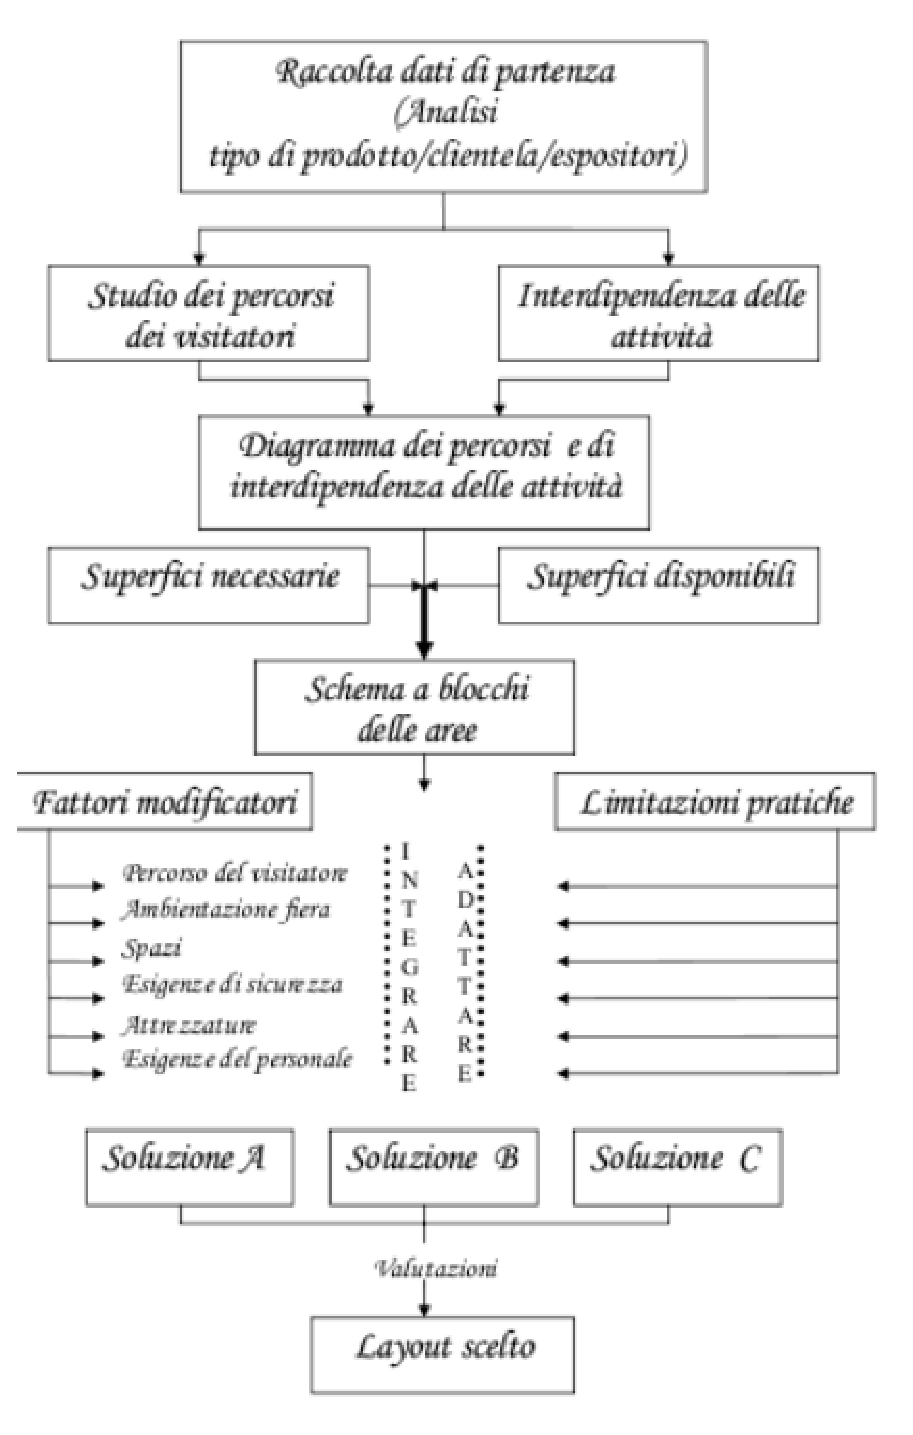
\includegraphics[width=13cm, height=21.5cm]{images/schema.eps}
\textit{\caption{\footnotesize Semplificazione concettuale di un generico knapsack problem}}
\end{figure}
Grazie all'aiuto della Ricerca Operativa\footnote{settore della matematica che si occupa prevalentemente di problemi di ottimizzazione di risorse, con largo uso di supporti matematici e informatici per la determinazione e l'applicazione di algoritmi di ottimizzazione} \`{e} possibile applicare delle metodologie di progetto adeguate al caso di layout fieristici. Nei prossimi paragrafi verranno introdotti alcuni importanti algoritmi per risolvere problemi legati al \textit{cutting} e \textit{packing} di oggetti e pi\`{u} in generale per determibare il layout ottimo. 

\section{Cutting and Packing problems}
L'ottimizzazione combinatoria \`{e} una branchia della Ricerca Operativa cui fanno riferimento i problemi di cutting e packing, i quali consistono nel trovare una soluzione massimizzata o minimizzata per mettere insieme un dato insieme di oggetti in uno o pi\`{u} contenitori.
Questa metodologia \`{e} molto utilizzata dalle industrie manifatturiere (legno, carta, vetro, acciaio, pelle, ecc.) cos\`{i} come nelle tipografie per la stampa di giornali e quotidiani, ma anche in molti altri settori della produzione industriale. Per molti anni si sono cercate soluzioni che minimizzassero il \textit{throughput}\footnote{numero di unit\`{a} completate in un certo lasso di tempo.} e i tempi di latenza\footnote{tempo impiegato per la produzione di un bene materiale o di un servizio offerto.} dei prodotti da ultimare, ma che nel contempo massimizzassero le quantit\`{a} e i volumi di produzione delle aziende. Settori ingegneristici della Ricerca Operativa, della \textit{Computer Science} o dell'industria manifatturiera si sono a lungo occupati di \textbf{problemi di cutting and packing (C \& P)}.\\
Basandosi su diversi criteri, uno su tutti legato alla \textbf{dimensione} del problema, si possono suddividere gli approcci progettuali in tre dimensioni. Trattandosi di layout fieristici, il nostro interesse si soffermer\`{a} solamente su due dimensioni, relativamente all'area espositiva della fiera.\\
\\
\begin{itemize}
\centering
\item \textbf{\textsc{C \& P problems ad una dimensione}}
\begin{enumerate}
\centering
\item Knapsack algorithm $01$ (KP)
\item Bin packing problem (BPP)
\end{enumerate}
\item \textbf{\textsc{C \& P problems a due dimensioni}}
\begin{enumerate}
\centering
\item Two-dimensional Bin Packing Problem (2BPP)
\item Two-dimensional Strip Packing Problem (2SPP)
\item Two-dimensional Knapsack Problem (2KP)
\end{enumerate}
\end{itemize}
E' necessario sottolineare che il \textit{cutting and packing} si pu\`{o} considerare valido e attuabile nel caso in cui le dimensioni degli oggetti interessati (\textit{items}) possano essere contenuti dagli oggetti contenitori (\textit{containers}) e che entrambi items e containers non si sovrappongano tra loro.
\subsection{Knapsack problem}
Supponendo, tra varie alternative, il caso in cui si debbano scegliere degli oggetti compatibilmente con certi criteri prestabiliti, consideriamo nella fattispecie il caso in cui, per restare in tema, si debbano scegliere tra gli stands quelli adatti alle nostre specifiche di layout. Se numeriamo gli stand "`"`idonei"'"' da $1$ a $n$ e creiamo un vettore di variabili binarie $x_{j} (j = 1,...,n)$ in modo che valga
$$ 
x_{j} =  
\left\{
\begin{array}{rl}
1 & \mbox{se l'oggetto j \`{e} scelto}\\
0 & \mbox{altrimenti}
\end{array}
\right.
$$
Se inoltre indichiamo con $p_{j}$ il profitto dato dall'oggetto $j$ (lo stand nel nostro caso), con $w_{j}$ la sua dimensione e con $c$ la dimensione del suo \textit{container} (ossia il suo \textit{costo}), allora l'obiettivo Knapsack sar\`{a} quello di selezionare, tra tutti, i vettori binari $x$ che soddisfano il vincolo $$\sum^{n}_{j=1}w_{j}x_{j} \leq c$$ e che massimizzano la funzione obiettivo $$\sum^{n}_{j=1}p_{j}x_{j}.$$
Per generalizzare il problema chiamiamo gli oggetti \textit{items}, con una quantit\`{a} pari ad $n$; il valore e la dimensione dell'oggetto $j-esimo$ sono chiamati rispettivamente \textit{profitto} e \textit{peso} e indicati con $p_{j}$ e $v_{j}$ ($j = (1,...,n)$).
Naturalmente il discorso appena fatto riguarda un caso knapsack generico, il cui scopo consiste nel determinare uno o pi\`{u} sottoinsiemi per cui la somma dei pesi non superi (o eguagli) una certa quantit\`{a} limite (detta \textit{bound}) e la somma dei valori sia massimizzata. Questa tipologia di problema, riconducibile all'\textbf{algoritmo Knapsack}, ha riscontrato enorme interesse da entrambi i punti di vista teorico e pratico, adattandosi a varie forme di progettazione che richiedono l'ottimizzazione.\\
Di seguito si analizzeranno pi\`{u} in dettaglio le varie tipologie di \textit{Cutting and Packing problems} in base alle definizioni precedentemente fornite per problemi a una e due dimensioni.
\subsubsection{KNAPSACK 0-1 (BINARY)}
Il \textit{Knapsack problem 0-1} \`{e} il pi\`{u} importante dei problemi di ottimizzazione combinatoria. Esiste un esempio di problema associato allo knapsack che ne esplica in maniera piuttosto esauriente la funzione. Tale problema, detto "`"`dello zaino"'"'\footnote{in inglese \textit{knapsack} indica proprio la parola \textit{zaino}} \`{e} posto nel modo seguente:
\begin{quotation}
\emph{sia dato uno zaino che possa supportare un determinato peso e siano dati inoltre N oggetti, ognuno dei quali caratterizzato da un peso e un'utilit\`{a} (ovvero un guadagno). Il problema si propone di scegliere quali di questi oggetti mettere nello zaino per ottenere la maggiore utilit\`{a} senza eccedere nel peso sostenibile dallo zaino stesso},
\end{quotation} 
il quale non \`{e} altro che un problema analogo al caso visto in precedenza.\\
Detto ci\`{o} si pu\`{o} proseguire elencando tre motivi fondamentali per cui l'algoritmo ha assunto tale importanza:
\begin{itemize}
\item pu\`{o} essere trattato come un semplice problema di Programmazione Intera Lineare (ILP)
\item appare come sottoproblema di problemi pi\`{u} complessi
\item pu\`{o} essere utile in molte soluzioni pratiche
\end{itemize}
\begin{figure}
\centering
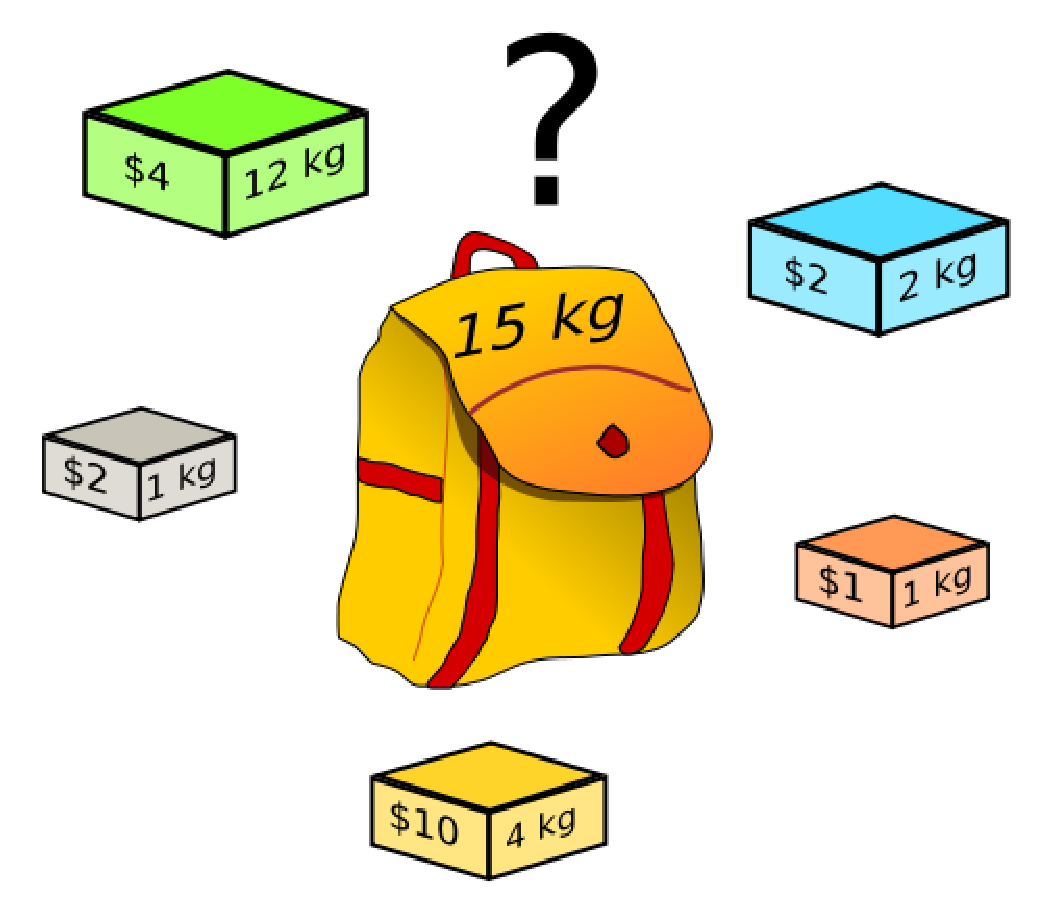
\includegraphics[width=10cm, height=8cm]{images/Knapsack.eps}
\textit{\caption{\footnotesize semplificazione concettuale di un generico knapsack problem}}
\end{figure}
Le variabili d'interesse per lo sviluppo di questo algoritmo sono tutte binarie (da qui il nome "`"`Knapsack 0-1"'"') e il succo del discorso pu\`{o} essere riassunto qui di seguito:\\
date le seguenti variabili
$$p_{j} = \mbox{profitto dell'oggetto j}$$ $$w_{j} = \mbox{peso dell'oggetto j}$$ $$c = \mbox{capacita del contenitore}$$
\`{e} opportuno scegliere un sottoinsieme di \textit{items} tale da:
\begin{equation}\label{eq1} \mbox{massimizzare} \longrightarrow max(z) = \sum^{n}_{j=1}p_{j}x_{j} \end{equation}
\begin{equation}\label{eq2} \mbox{soddisfacendo} \longrightarrow \sum^{n}_{j=1}w_{j}x_{j} \leq c \end{equation}
\begin{equation}\label{eq3} \mbox{dove} \longrightarrow x_{j}\in \left\lbrace 0,1\right\rbrace , j \in N =\left\lbrace1,...,n\right\rbrace \end{equation}
analogamente alle definizioni date in precedenza.\\
Se ora ipotizziamo che
\begin{equation}\label{eq4} p_{j}, w_{j} \mbox{e } c \mbox{ sono interi positivi,} \end{equation}
\begin{equation}\label{eq5} \sum^{n}_{j=1}w_{j}\leq c, \end{equation}
\begin{equation}\label{eq6} w_{j} < c , \mbox{con } j \in N, \end{equation}
e se consideriamo violata la prima ipotesi, allora si ottengono delle frazioni che possono essere moltiplicate per un opportuno fattore, mentre gli eventuali valori negativi verranno trattati come $0$ o come $1$ in base alle seguenti relazioni:
\begin{itemize}
\item $\forall j \in N^{0} = \left\lbrace j \in N : p_{j} \leq 0, w_{j} \geq 0 \right\rbrace \Longrightarrow x_{j}=0$
\item $\forall j \in N^{1} = \left\lbrace j \in N : p_{j} \geq 0, w_{j} \leq 0 \right\rbrace \Longrightarrow x_{j}=1$
\end{itemize}
Definiamo inoltre $N^{-}$ come $N^{-} = \left\lbrace j\in N : p_{j}<0, w_{j}>0\right\rbrace$, mentre per $N^{+}$ il valore sar\`{a}: $N^{+}= N \setminus (N^{0}\cup N^{1}\cup N^{-})$.\\
Infine definiamo:
$$ 
\left\{
\begin{array}{ll}
y_{j} = 1 - x_{j},  \bar{p}_{j} = - p_{j}, \bar{w}_{j} = - w_{j} & \mbox{per }  j \in N^- \\
y_{j} = x_{j}, \bar{p}_{j} = p_{j}, \bar{w}_{j}=w_{j} & \mbox{per }  j \in N^+
\end{array}
\right.
$$
Ora che tutte le variabili e i casi sono stati definiti, enunciamo il problema. Si vuole risolvere il problema che ha come obiettivo quello di massimizzare la funzione $$z = \sum_{j \in N^{-} \cup N^{+}} \bar{p}_{j} y_{j} + \sum_{j \in N^{1} \cup N^{-}} p_{j}$$
mentre come \textit{constraint} del problema la funzione $$\sum_{j \in N^{-} \cup N^{+}} \bar{w}_{j} y_{j} \leq c - \sum_{j \in N^{1} \cup N^{-}} w_{j}.$$
Se i dati in input violano l'espressione (1.2) ipotizzata precedentemente allora $x_{j} = 0 , \forall j \in N$, mentre se violano l'assunzione (1.3) allora si avr\`{a} $x_{j} = 0 , \forall j \in N : w_{j} > c$ .\\
Se non specificato in altro modo, si supporranno sempre gli \textit{items} in ordine decrescente secondo l'ordine del profitto per unit\`{a} di peso:
$$\dfrac{p_{1}}{w_{1}} \geq \dfrac{p_{2}}{w_{2}} \geq ... \geq \dfrac{p_{n}}{w_{n}} $$
Data ad ogni problema una \textit{istanza} $I$, si indicher\`{a} il valore di ogni soluzione ottima con $z(I)$ o pi\`{u} semplicemente con $z$.
Considerando il problema nella versione minimizzata anzich\`{e} massimizzata, gli obiettivi si invertono secondo lo schema seguente:
$$\mbox{minimizzare} \longrightarrow min(z) = \sum^{n}_{j=1}p_{j}y_{j}$$
$$\mbox{soddisfacendo} \longrightarrow \sum^{n}_{j=1}w_{j}y_{j} \leq q$$
$$\mbox{dove} \longrightarrow y_{j}\in \left\lbrace 0,1\right\rbrace , j \in N =\left\lbrace1,...,n\right\rbrace$$
dal quale si evince che il procedimento per tornare da una forma (minimizzata) all'altra (massimizzata) consiste nel porre $y_{j} = 1 - x_{j}$ e risolvendo la (1.1), la (1.2) e la (1.3) con $c = \sum^{n}_{j=1}w_{j} - q$.\\
Inoltre, ponendo come $z_{max}$ il valore della soluzione massimizzata di ogni problema, la sua versione minimizzata sar\`{a} $z_{min} = \sum^{n}_{j=1}p_{j} - z_{max}$.\\
\\
\underline{Rilassamento lineare}\\
Togliendo il vincolo dell'integrit\`{a} sulle variabili $x_{j}$, nelle propriet\`{a} (1.1), (1.2) e (1.3), si ottiene la prima variante del problema knapsack 0-1 ovvero il cosiddetto \textit{rilassamento lineare} o \textit{continuous Knapsack problem C(KP)}. In pratica un rilassamento \`{e} una qualunque tecnica che ha lo scopo di migliorare (ottimizzare) la funzione obiettivo in tutti i punti della regione ammissibile originale\footnote{metodo improntato sull'ampliamento della regione ammissibile e/o sull'innalzamento della funzione obiettivo in corrispondenza della regione ammissibile originale}: 
$$\mbox{massimizzare} \longrightarrow max(z) = \sum^{n}_{j=1}p_{j}x_{j}$$
$$\mbox{soddisfacendo} \longrightarrow \sum^{n}_{j=1}w_{j}x_{j} \leq c$$
$$\mbox{dove} \longrightarrow 0 \leq x_{j} \leq 1 , j = 1,...,n$$ 
Supponiamo inoltre che gli oggetti, ordinati come illustrato sopra, siano inseriti consecutivamente nel contenitore, finch\'{e} non si trova un oggetto $s$ che non pu\`{o} pi\`{u} essere inserito. Questo \`{e} un problema di \textit{critical item}:
$$s = \left\lbrace j : \sum^{j}_{i=1} w_{j} > c \right\rbrace$$ 
da cui si pu\`{o} notare, ricordando le (1.4), (1.5) e (1.6), che si ha $1 < s \leq n$.\\
Tale metodo \`{e} stato risolto nel 1957 mediante un algoritmo scoperto da Dantzig.\\
\\
\underline{Rilassamento lagrangiano}\\
Un'alternativa al caso appena visto, di tipo lineare, \`{e} il rilassamento lagrangiano. In questo modo ci si pone lo scopo di eliminare un insieme di vincoli, tenendone per\`{o} conto nella funzione obiettivo.\\
Dato un fattore non negativo $\lambda$, il \textit{rilassamento lagrangiano} del KP, indicato con (L(KP, $\lambda$)) \`{e}:
$$\mbox{massimizzare} \longrightarrow max(z) = \sum^{n}_{j=1}p_{j}x_{j} + \lambda (c - \sum^{n}_{j=1} w_{j}x_{j})$$
$$\mbox{dove} \longrightarrow x_{j} \in \left\lbrace 0,1\right\rbrace , j = 1,...,n.$$
La funzione obiettivo pu\`{o} essere espressa come
\begin{equation}\label{eq7}
z(L(KP, \lambda)) = \sum^{n}_{j=1}\tilde{p}_{j}x_{j} + \lambda c
\end{equation} 
dove $\tilde{p}_{j} = p_{j} + \lambda w_{j}$ per $j=1,...,n$. La soluzione ottima di $L(KP,\lambda)$ \`{e} facilmente determinabile in un tempo $O(n)$ come:
\begin{equation}\label{eq8}
\tilde{x}_{j} =
\left\{
\begin{array}{rl}
1 & \mbox{se } \tilde{p}_{j}>0 \\
0 & \mbox{se } \tilde{p}_{j}<0
\end{array}
\right.
\end{equation}
(quando $\tilde{p}_{j} = 0$ il valore di $x_{j}$ \`{e} irrilevante).\\
Quindi, definendo $ J(\lambda)= \left\lbrace j : \dfrac{\tilde{p}_{j}}{w_{j}} > \lambda \right\rbrace $, il valore della soluzione $L(KP, \lambda)$ sar\`{a}:
$$z(L(KP, \lambda)) = \sum_{j \in J(\lambda)}\tilde{p}_{j} + \lambda c.$$
Per ogni $\lambda \geq 0$ c'\`{e} un upper bound in $z(KP)$ che, comunque, non potr\`{a} mai essere migliore della soluzione fornita da Dantzig; l'equazione (1.8) ci fornisce la soluzione del rilassamento continuo (o lagrangiano) di $L(KP, \lambda)$ nel modo seguente:
$$z(L(KP, \lambda)) = z(C(L(KP, \lambda))) \geq z(C(KP))$$
Il valore di $\lambda$ che produce il valore minimo di $z(L(KP, \lambda))$ \`{e} $\lambda^{*} = \frac{p_{s}}{w_{s}}$. Con questo valore, in realt\`{a}, abbiamo che $\tilde{p}_{j} \geq 0$ per $j=1,...,s-1$  mentre $\tilde{p_{j}} \leq 0$ per $j=s,...,n$. In questo modo $J(\lambda^{*}) \subseteq \left\lbrace 1,...,s-1 \right\rbrace$.\\ Da qui $\tilde{x_{j}} = \bar{x}_{j}$, per $j \in N \setminus \left\lbrace s \right\rbrace $
(dove $\bar{x}_{j}$ \`{e} definita nel teorema seguente) e grazie alle (1.7) e (1.8), si evince che
$$z(L(KP, \lambda^{*})) = \sum_{j=1}^{s-1} (p_{j} - \lambda^{*}w_{j}) + \lambda^{*}c = z(C(KP))$$
Infine si pu\`{o} notare che, per $\lambda = \lambda^{*}$, $\tilde{p}_{j}$ diventa $p^{*}_{j} = p_{j} - w_{j} \dfrac{p_{s}}{w_{s}}$; il modulo $|p_{j}^{*}|$ \`{e} il decremento che si ottiene in $z(L(KP, \lambda^{*}))$ ponendo $\tilde{x}_{j} = 1 - x_{j}$ e da qui un lower bound sul corrispondente decremento della soluzione continua (da quando l'ottimo $\lambda$ cambia imponendo le condizioni sopra elencate).
Altri rilassamenti lagrangiani del problema KP sono stati studiati da Maculan (1983) e da Fisher (1981).\\
\\
\underline{Teorema}\\
La soluzione ottima $\bar{x}$ del problema C(KP) \`{e}:
$$\bar{x}_{j} = 1 \mbox{ per } j = 1,...,s-1$$ $$\bar{x}_{j} = 0 \mbox{ per } j = s+1,...,n$$ $$\bar{x}_{s} = \dfrac{\bar{c}}{w_{s}},$$ dove: $$\bar{c}=c - \sum_{j=1}^{s-1} w_{j}.$$ \\
\begin{figure}[h]
\centering
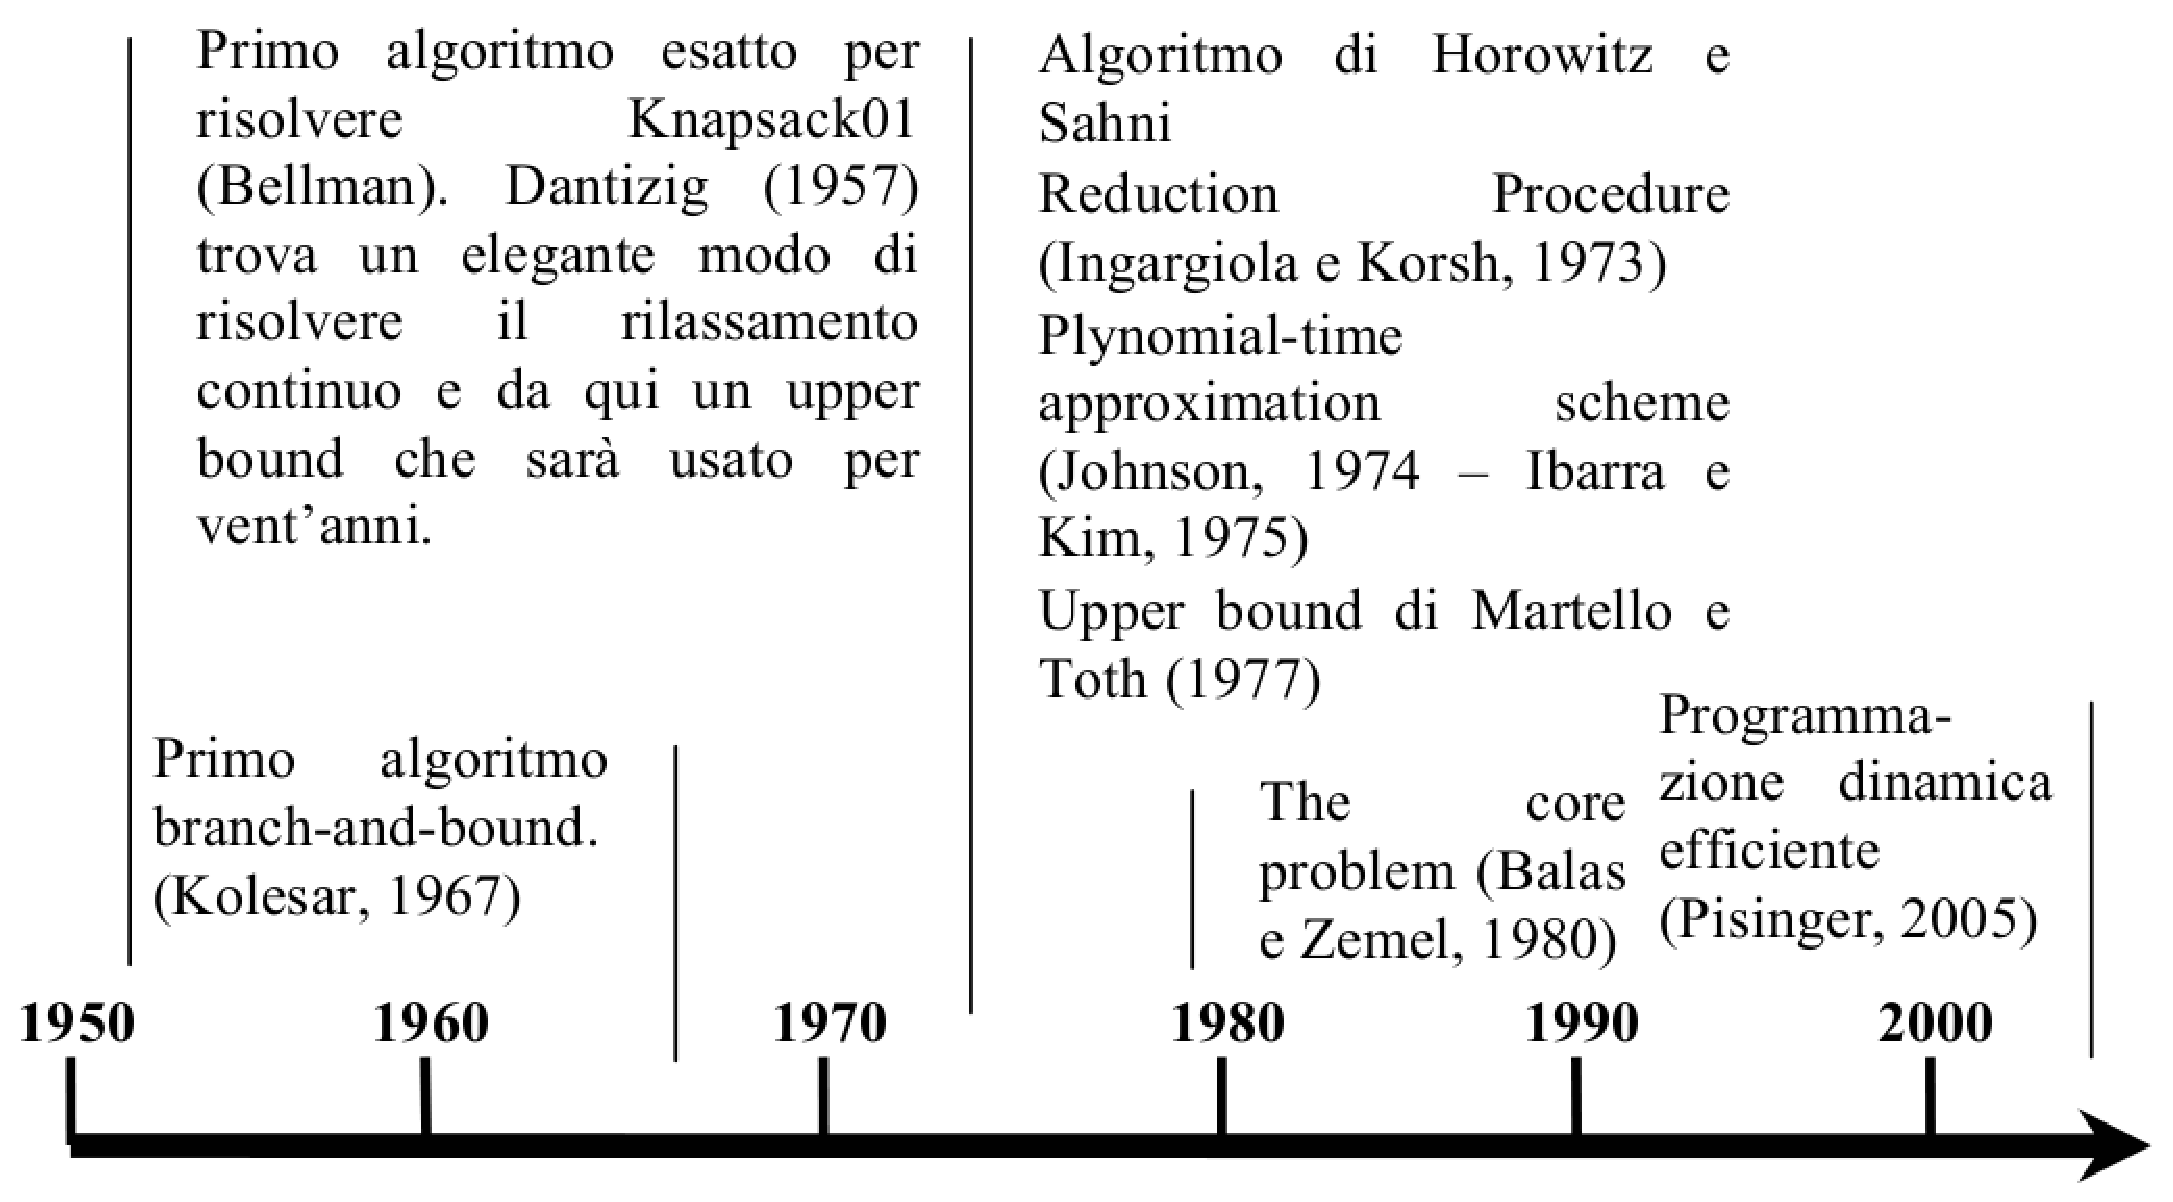
\includegraphics[width=14cm, height=8cm]{images/cronologia.eps}
\textit{\caption{\footnotesize scoperte e applicazioni pi\`{u} importanti legate ai modelli knapsack problem in ordine cronologico}}
\end{figure}\\
\subsection{Bin Packing Problem}
Il bin-packing problem (BPP) \`{e} un altro tipo di problema di natura combinatoria e consiste nel raggruppare oggetti di volumi diversi in un numero finito di compartimenti di capacit\`{a} $V$, in maniera tale da minimizzare il numero di tali compartimenti da utilizzare. 
\begin{figure}[h]
\centering
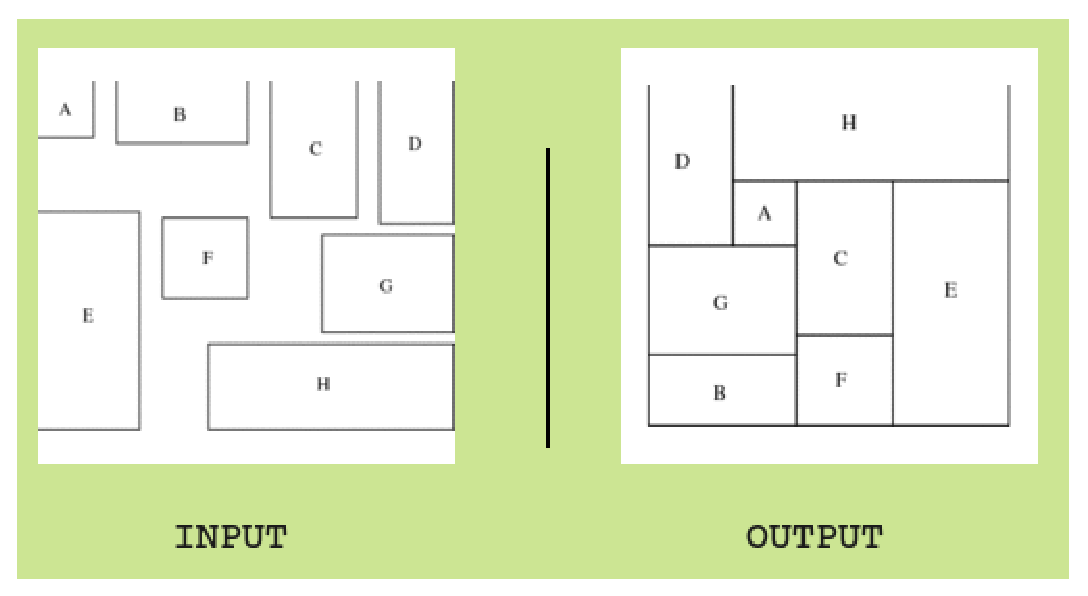
\includegraphics[width=11cm, height=6cm]{images/binpacking.eps}
\textit{\caption{\footnotesize Bin Packing Problem}}
\end{figure}
\\Ovviamente, come per tutti i problemi di questo tipo, anche il BPP ha un campo di applicazione molto vasto, dall'industria ai trasporti, dalla logistica all'organizzazione aziendale, dall'informatica alle telecomunicazioni. 
Usando la terminologia e la formalizzazione tipiche dei problemi \textit{knapsack}, indichiamo con $n$ il numero di oggetti/items e di contenitori (\textit{bins}) mentre indicheremo con $w_{j}$ il peso dell'\textit{item} j-esimo e con $c$ la capacit\`{a} di ogni \textit{bin}.\\
Lo scopo del problema \`{e} di assegnare ogni item ad un bin in modo che il peso totale degli oggetti in ogni contenitore non ecceda la capacit\`{a} $c$ del contenitore stesso, e che il numero dei bins impiegati sia minimo.\\
Dal punto di vista matematico, il problema si pone nel modo seguente:
$$\mbox{minimizzare} \longrightarrow min(z) = \sum^{n}_{i=1}y_{i}$$
$$\mbox{soddisfacendo} \longrightarrow \sum^{n}_{j=1}w_{j}x_{ij} \leq c y_{i}, i \in N = \left\lbrace 1,...,n\right\rbrace ,$$ 
$$\sum_{i=1}^{n} x_{ij} = 1, j\in N,$$  $$y_{j} \in \left\lbrace 0,1 \right\rbrace, i \in N,$$ $$x_{ij} \in \left\lbrace 0,1 \right\rbrace, i,j \in N$$
Si definiscono qui di seguito i valori delle variabili:
\begin{equation}\label{eq9}
y_{i}
\left\{
\begin{array}{ll}
1 \mbox{ se il bin i \`{e} usato} \\
0 \mbox{ altrimenti}
\end{array}
\right.
\end{equation}
\begin{equation}\label{eq10}
x_{ij}
\left\{
\begin{array}{ll}
1 \mbox{ se l'item j \`{e} assegnato al contenitore i} \\
0 \mbox{ altrimenti}
\end{array}
\right.
\end{equation}
$$c \mbox{ \`{e} un intero positivo}$$
\begin{equation}\label{eq11}
w_{j} \geq c \mbox{ per } j\in N
\end{equation}
Se l'assunzione (\ref{eq11}) risulta violata e i $w_{j}$ sono tutti interi, $c$ pu\`{o} essere sostituito con $\lfloor c \rfloor$ ; se un item viola l'assunzione (\ref{eq12}) l'istanza risulta inaccettabile. Tuttavia non esiste un modo semplice per trasformare una istanza in modo da poter trattare pesi negativi. Per semplicit\`{a} assumiamo che, per ogni soluzione ammissibile, vengano usati i \textit{bins} di indice pi\`{u} basso (ad esempio $y_{i} \leq y_{i+1}$ per $i = 1,...,n-1$).\\
L'approccio mediante algoritmi BPP viene trattato in letteratura basandosi sulla approssimazione degli algoritmi stessi e sulle loro performance. In questo campo rivestono particolare importanza gli studi di Coffman, Garey e Johnson (1984).\\
\\
\underline{Algoritmi approssimati}\\
Il pi\`{u} semplice approccio approssimativo al \textit{bin-packing problem} \`{e} l'algoritmo \textbf{Next-Fit} (NF): il primo oggetto/item \`{e} assegnato al bin 1. Gli items $2,...,n$ sono poi consideati al crescere dell'indice, ossia ogni item \`{e} assegnato al bin corrente se adatto, altrimenti \`{e} assegnato a un nuovo bin che diventa quello corrente. Si deduce che la complessit\`{a} dell'algoritmo \`{e} $O(n)$\footnote{in ambito computazionale, in relazione a una teoria della complessit\`{a}, la notazione detta \textit{big O} \`{e} usata per descrivere quanto la dimensione, il peso dell'input influisce sulle risorse impiegate nell'elaborazione di un algoritmo (di solito sui tempi di throughput o dell'occupazione di memoria)}. E' facile infatti provare che, per ogni isanza $I$ del BPP, la soluzione $NF(I)$ fornita dall'algoritmo soddisfa il bound $$NF(I) \leq 2 z(I)$$
dove $z(I)$ indica la soluzione ottima. Esistono, inoltre, istanze per cui il rapporto $\dfrac{NF(I)}{z(I)}$ tra le due soluzioni \`{e} arbitrariamente fermato a 2: cio\`{e} la peggior performance che si possa avere nel rapporto di NF \`{e} che $r(NF = 2)$. Si nota che, per un problema di minimo, il peggior caso di un rapporto tra un generico algoritmo A approssimato \`{e} definito come il pi\`{u} piccolo numero $r(A) \in R$ tale che $$\dfrac{A(I)}{z(I)} \leq r(A) \mbox{ per tutte le istanze di I, }$$ dove A(I) indica la soluzione ottenuta dall'algoritmo A.\\
\\Un algoritmo migliore, il \textbf{First-Fit} (FF), considera gli items all'incrementare degli indici e assegna ogni item al pi\`{u} basso indice di bin inizializzato nel quale entra; solo quando l'oggetto corrente non viene assegnato a qualche bin inizializzato, viene introdotto un nuovo contenitore.\\
\\Un altro algoritmo, \textbf{Best-Fit} (BF), \`{e} ottenuto dal FF assegnando il corrente item al bin accettabile (se c'\`{e}) che ha la pi\`{u} piccola capacit\`{a} residua (rompendo il vincolo del bin con indice pi\`{u} basso).\\
\\Si assuma ora che gli oggetti siano sistemati in modo che siano $w_{1} \leq w_{2} \leq ... \leq w_{n}$, e che in seguito siano applicati gli algoritmi NF, oppure FF, oppure BF. Gli algoritmi risultanti sono chiamati rispettivamente \textbf{Next-Fit Decreasing} (NFD), \textbf{First-Fit Decreasing} (FFD) e \textbf{Best-Fit Decreasing} (BFD).\\
\\La complessit\`{a} di questi algoritmi e i casi peggiori di performance che si possono raggiungere sono stati studiati da Johnson, Demers, Ullman, Garey e Graham (1974).\\
\\Nella tabella riassuntiva di fig. 1.5 sono illustrati i criteri di valutazione dei vari algoritmi, in cui $r^{\infty}$ \`{e} l'\textit{asymptotic worst case performance ratio}\footnote{stima asintotica della prestazione nel caso peggiore; il simbolo di infinito sta ad indicare il numero imprecisato di volte per cui viene ripetuta la stima}; per un generico algoritmo approssimato A, esso \`{e} definito come il minor numero reale $r^{\infty}(A)$ tale che, per un qualche valore intero positivo K, sia $\dfrac{A(I)}{z(I)} \leq r^{\infty}(A)$ per ogni istanza I che soddisfi $z(I) \geq K$:  \\
\begin{figure}[h]
\centering
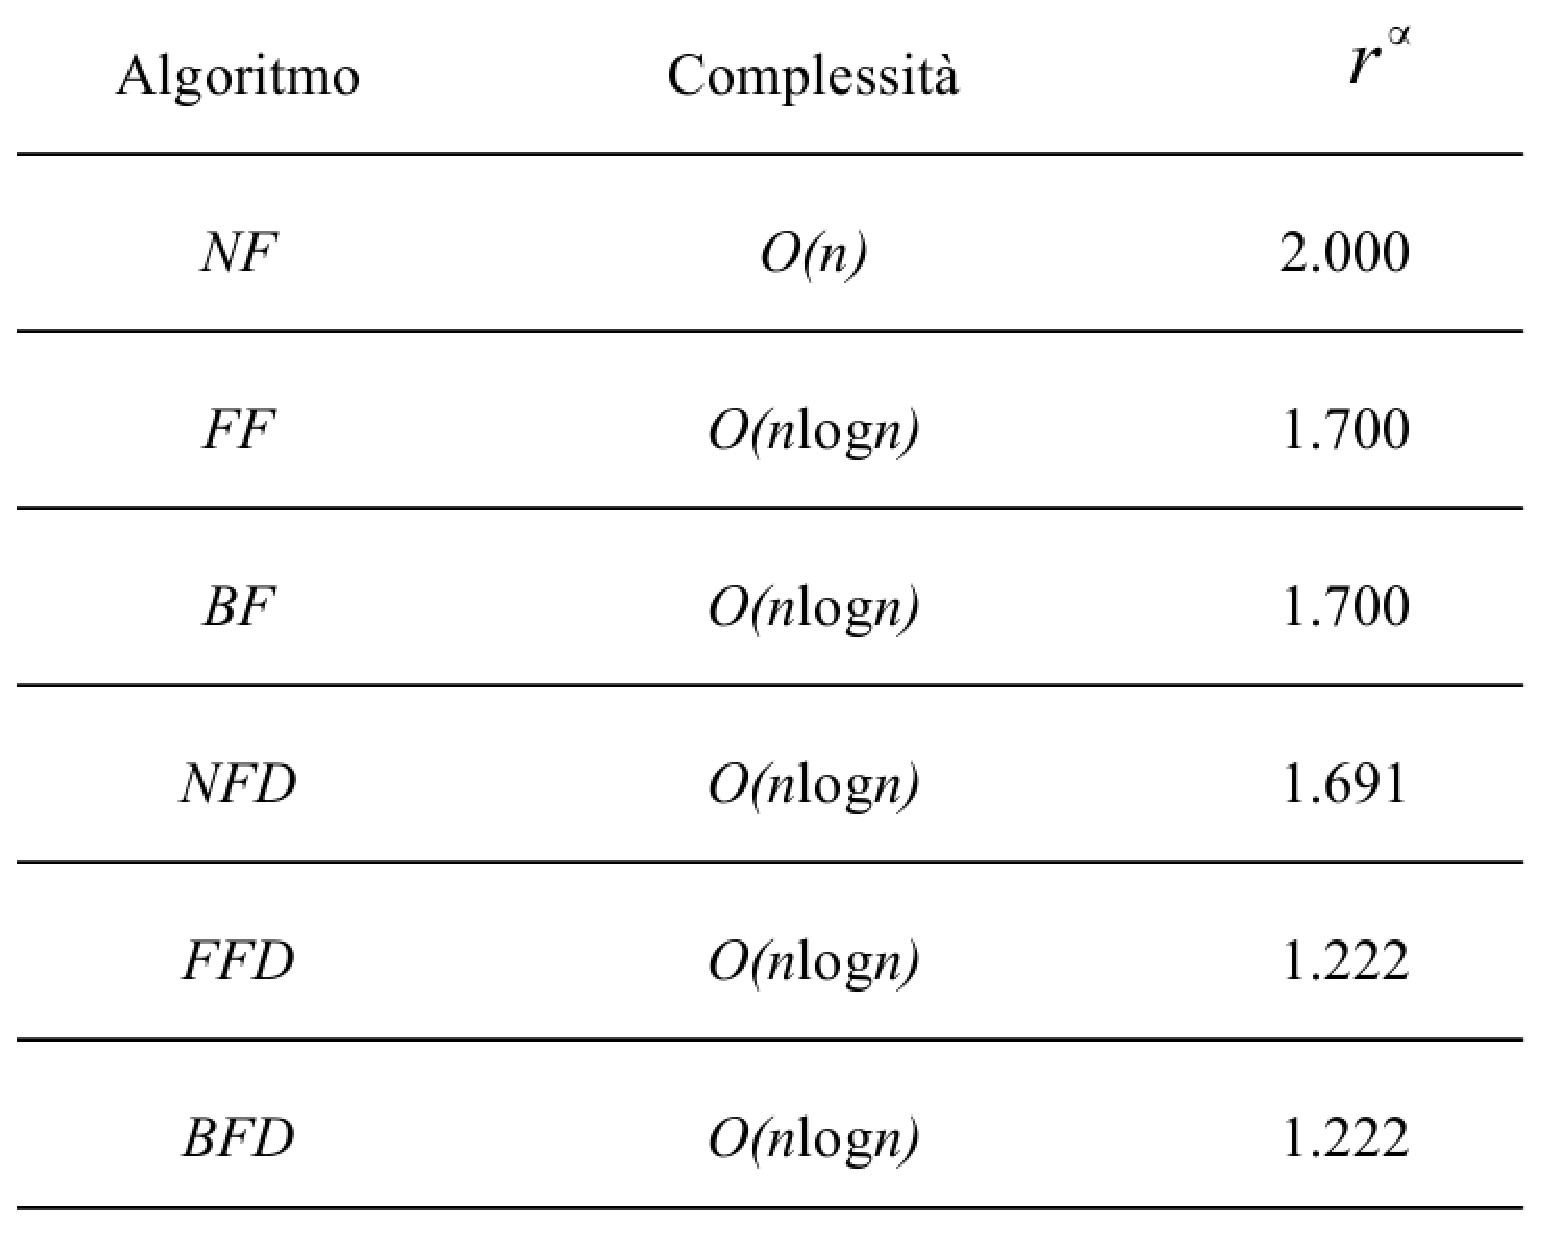
\includegraphics[width=9cm, height=7cm]{images/tabella.eps}
\textit{\caption{\footnotesize confronto tra i vari algoritmi e loro performance}}
\end{figure}\\
\\
\underline{Rilassamento lineare}\\
Enunciamo qui di seguito la versione del \textit{continuous problem} riferita al rilassamento lineare nel caso del bin packing. Per il modello in esame il C(BPP) \`{e} il seguente:
$$\mbox{minimizzare} \longrightarrow min(z) = \sum^{n}_{i=1}y_{i}$$
$$\mbox{soddisfacendo} \longrightarrow \sum^{n}_{j=1}w_{j}x_{ij} \leq c y_{i}, i \in N = \left\lbrace 1,...,n\right\rbrace ,$$ 
$$\sum_{i=1}^{n} x_{ij} = 1, j\in N,$$  $$0 \leq y_{i} \leq 1, i \in N,$$ $$ 0 \leq x_{ij} \leq 1 , i,j \in N$$
Tale rilassamento pu\`{o} essere facilmente risolto ponendo $x_{ij} = 1$, $x_{ij} = 0$ con $(j \not= j)$ e ponendo $y_{i}= \frac{w_{i}}{c}, \forall i \in N$. Da qui otteniamo $$z(C(BPP)) = \sum_{i=1}^{n} \frac{w_{i}}{c}$$
\subsection{Two Dimensional Bin-packing Problem}
Finora si sono classificati i problemi di packing a seconda del numero di dimensioni. In problemi BPP l'attenzione era focalizzata sull'obiettivo di trovare un modo per raggruppare insieme un certo numero di oggetti, impiegando il minor numero di contenitori possibile.\\ I problemi a due dimensioni possono anche essere classificati in base alla forma degli oggetti da impaccare; nelle applicazioni industriali \`{e} particolarmente presente il \textit{two-dimensional rectangle packing problem} per cui \`{e} richiesto di collocare un insieme di oggetti rettangolari in un numero minimo di unit\`{a} rettangolari pi\`{u} grandi, minimizzando quindi anche lo spazio inutilizzato. Inoltre nelle industrie del legno e del vetro, pezzi di forma rettangolare devono essere tagliati a partire da grandi lamine di materiale. Nel contesto dei magazzini, i prodotti devono essere messi sugli scaffali. Nell'impaginazione dei giornali, gli articoli devono essere ben posizionati nelle pagine. In tutte queste applicazioni industriali, il problema del packing si presenta spesso con vincoli lievemente differenti; molte varianti del problema sono state considerate in letteratura.\\
Contestualmente, quando si ha a che fare con problemi multi-dimensionali, si tende a raggrupparli nel cosiddetto insieme di problemi NP-hard\footnote{abbreviazione di \textit{Non-deterministic Polynomial time}; sono problemi decisionali la cui soluzione non pu\`{o} essere determinata mediante l'utilizzo di software e computazioni usuali, ma mediante approcci euristici} ossia una particolare classe di problemi non risolvibili mediante algoritmi polinomiali. 
Ovviamente, pi\`{u} aumentano la complessit\`{a} delle specifiche e pi\`{u} aumentano i vincoli da soddisfare:
\begin{itemize}
\item \textbf{Orientamento}\\ Si assume di solito che ogni rettangolo abbia una certa rotazione fissa, oppure che possa essere ruotato di $90^{\circ}$. La rotazione dei rettangoli non \`{e} ammessa per esempio nell'impaginazione dei giornali, quando gli item da tagliare sono decorati o non isomorfi (legno, lamiera).

\item \textbf{Tagli a ghigliottina}\\ Effettuare un taglio a ghigliottina significa che gli items sono stati ottenuti attraverso una sequenza di tagli lato-a-lato paralleli ai lati del contenitore. Ci\`{o} \`{e} spesso imposto da limitazioni tecniche di macchine da taglio automatiche ( ad esempio seghe verticali o circolari) o di alcuni materiali. in figura 1.6 sono illustrati due esempi di piazzamenti di items con o senza il vincolo dei tagli a ghigliottina.
 
\item \textbf{Impaccamento a livelli}\\ Il piazzamento degli items \`{e} ottenuto posizionandoli da sinistra a destra in righe formanti diversi livelli. Il primo livello \`{e} il fondo del contenitore, e ogni livello seguente \`{e} la linea orizzontale coincidente con il lato superiore dell'item pi\`{u} alto impaccato a livello inferiore. In figura 1.7 se ne presenta un dettaglio illustrativo.

\item \textbf{Checkerboard pattern}\\ I checkerboard patterns, conosciuti anche come \textit{1-group patterns} (Gilmore e Gomory, 1965) fanno parte della classe speciale dei tagli a ghigliottina a due fasi (\textit{two-stage guillotine patterns}) che non necessitano di essere ritagliati. Essi
possono infatti essere prodotti ruotando la sega di $90^{\circ}$, dopo i tagli fatti in una prima fase. Le strisce ottenute nella prima fase sono tutte tagliate nella seconda fase producendo gli items desiderati (illustrazione in figura 1.8). Tagli di questo tipo richiedono meno tempo per le macchine, e sono particolarmente interessanti nei settori con alta domanda quando le macchine rappresentano il collo di bottiglia della produzione.

\item \textbf{Packing Problem Unconstrained, Constrained o Doubly constrained} \\ Indicando con $x_{i}$ i pezzi da impaccare e con $P_{i}$ e $Q_{i}$ rispettivamente il minimo e massimo numero di oggetti di tipo $i$ da poter impaccare, si ha che $0 \leq P_{i} \leq x_{i} \leq Q_{i}$ e che in accordo con tali assunzioni si possono distinguere tre tipi di problemi:
\begin{enumerate}
\item \textit{Unconstrained}: $\forall i$, $P_{i}=0$, $Q_{i}= \lfloor \dfrac{L*W}{l_{i}*w_{i}} \rfloor$
\item \textit{Constrained}: $\forall i$, $P_{i}=0$, $Q_{i}< \lfloor \dfrac{L*W}{l_{i}*w_{i}} \rfloor$
\item \textit{Doubly Constrained}: $\exists i : P_{i}>0$, $\exists j : Q_{j}= \lfloor \dfrac{L*W}{l_{j}*w_{j}} \rfloor$
\end{enumerate}
\end{itemize}

\begin{figure}
\centering
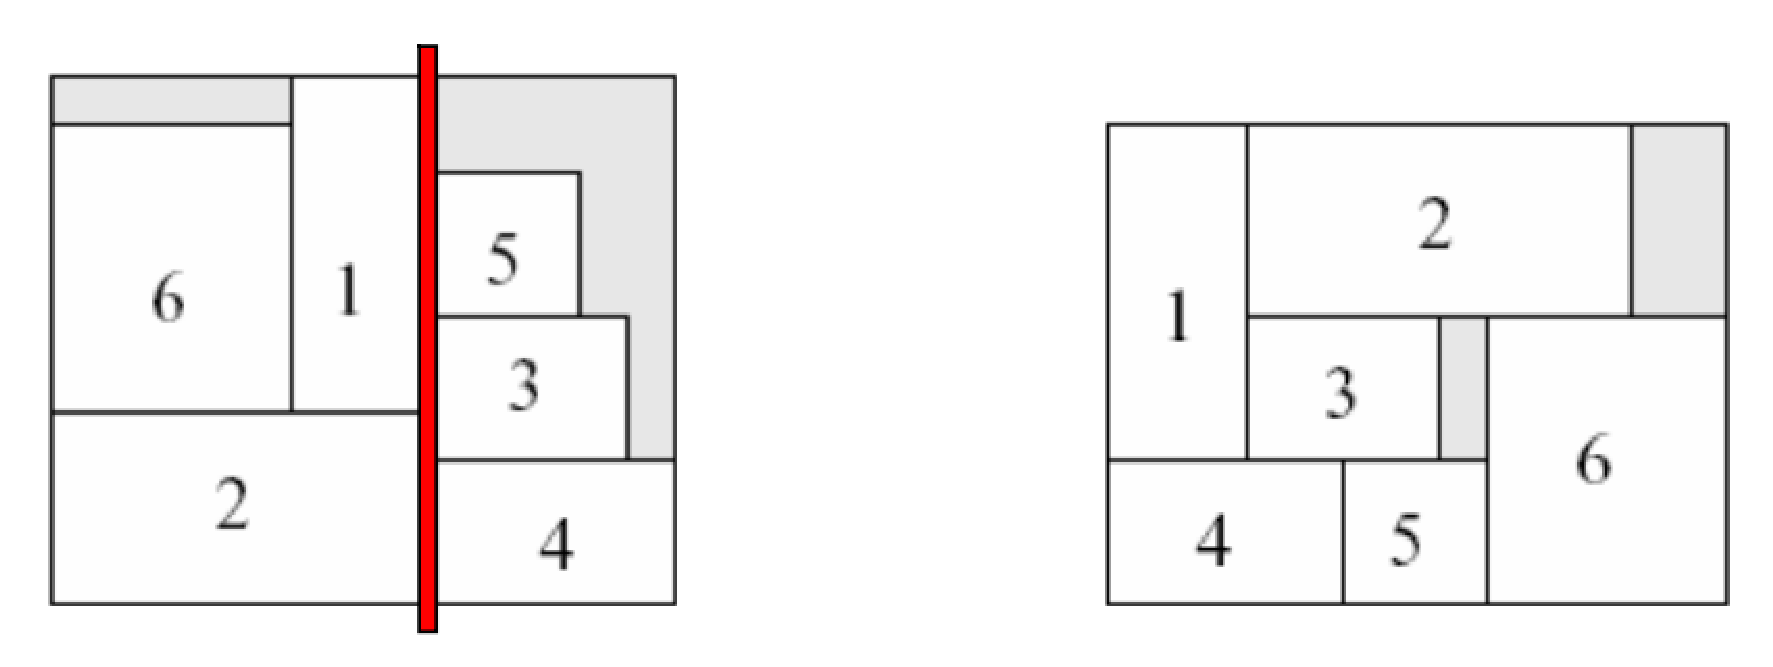
\includegraphics[width=9.5cm, height=4cm]{images/ghigliottina.eps}
\textit{\caption{\footnotesize taglio a ghigliottina: nel caso a sinistra il taglio, in quello a destra la disposizione originale}}
\end{figure}

\begin{figure}
\centering
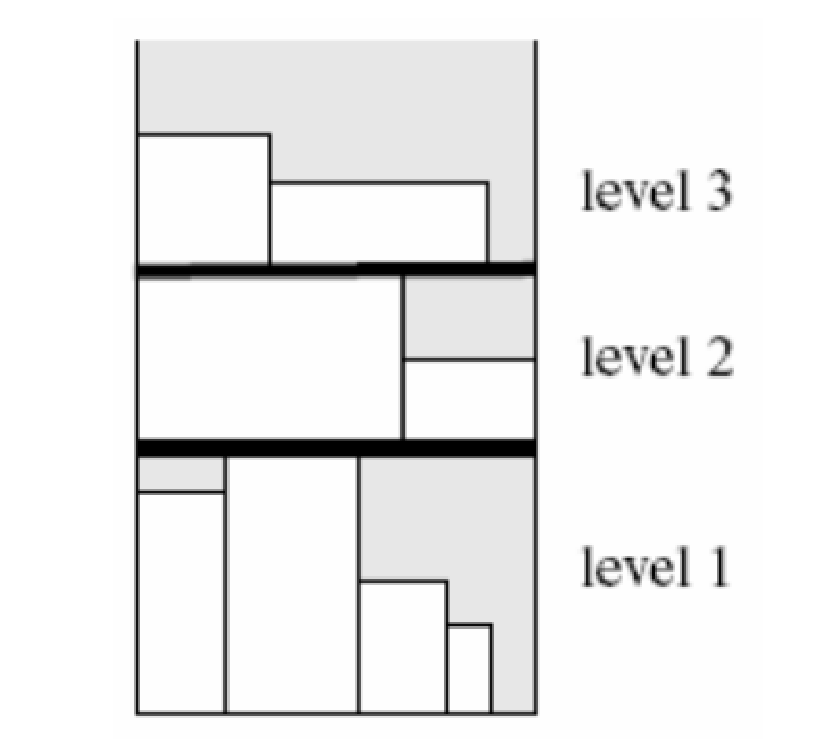
\includegraphics[width=8cm, height=6cm]{images/levelpack.eps}
\textit{\caption{\footnotesize level packing}}
\end{figure}

\begin{figure}
\centering
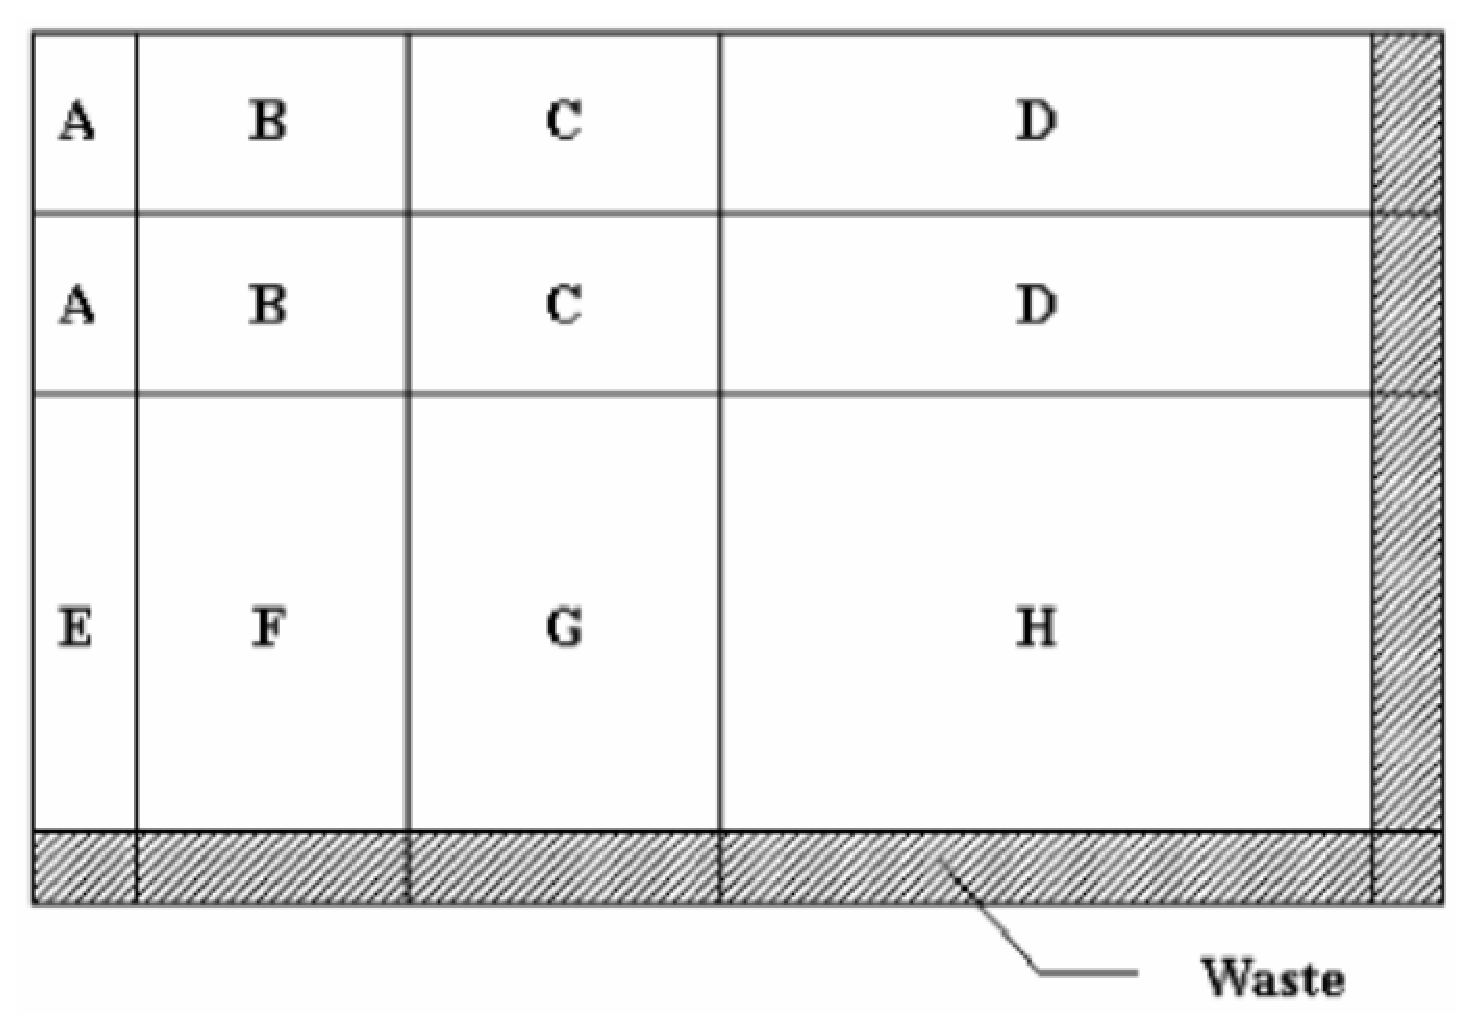
\includegraphics[width=8cm, height=6cm]{images/scacchi1.eps}
\textit{\caption{\footnotesize checkerboard pattern}}
\end{figure}

\begin{figure}
\centering
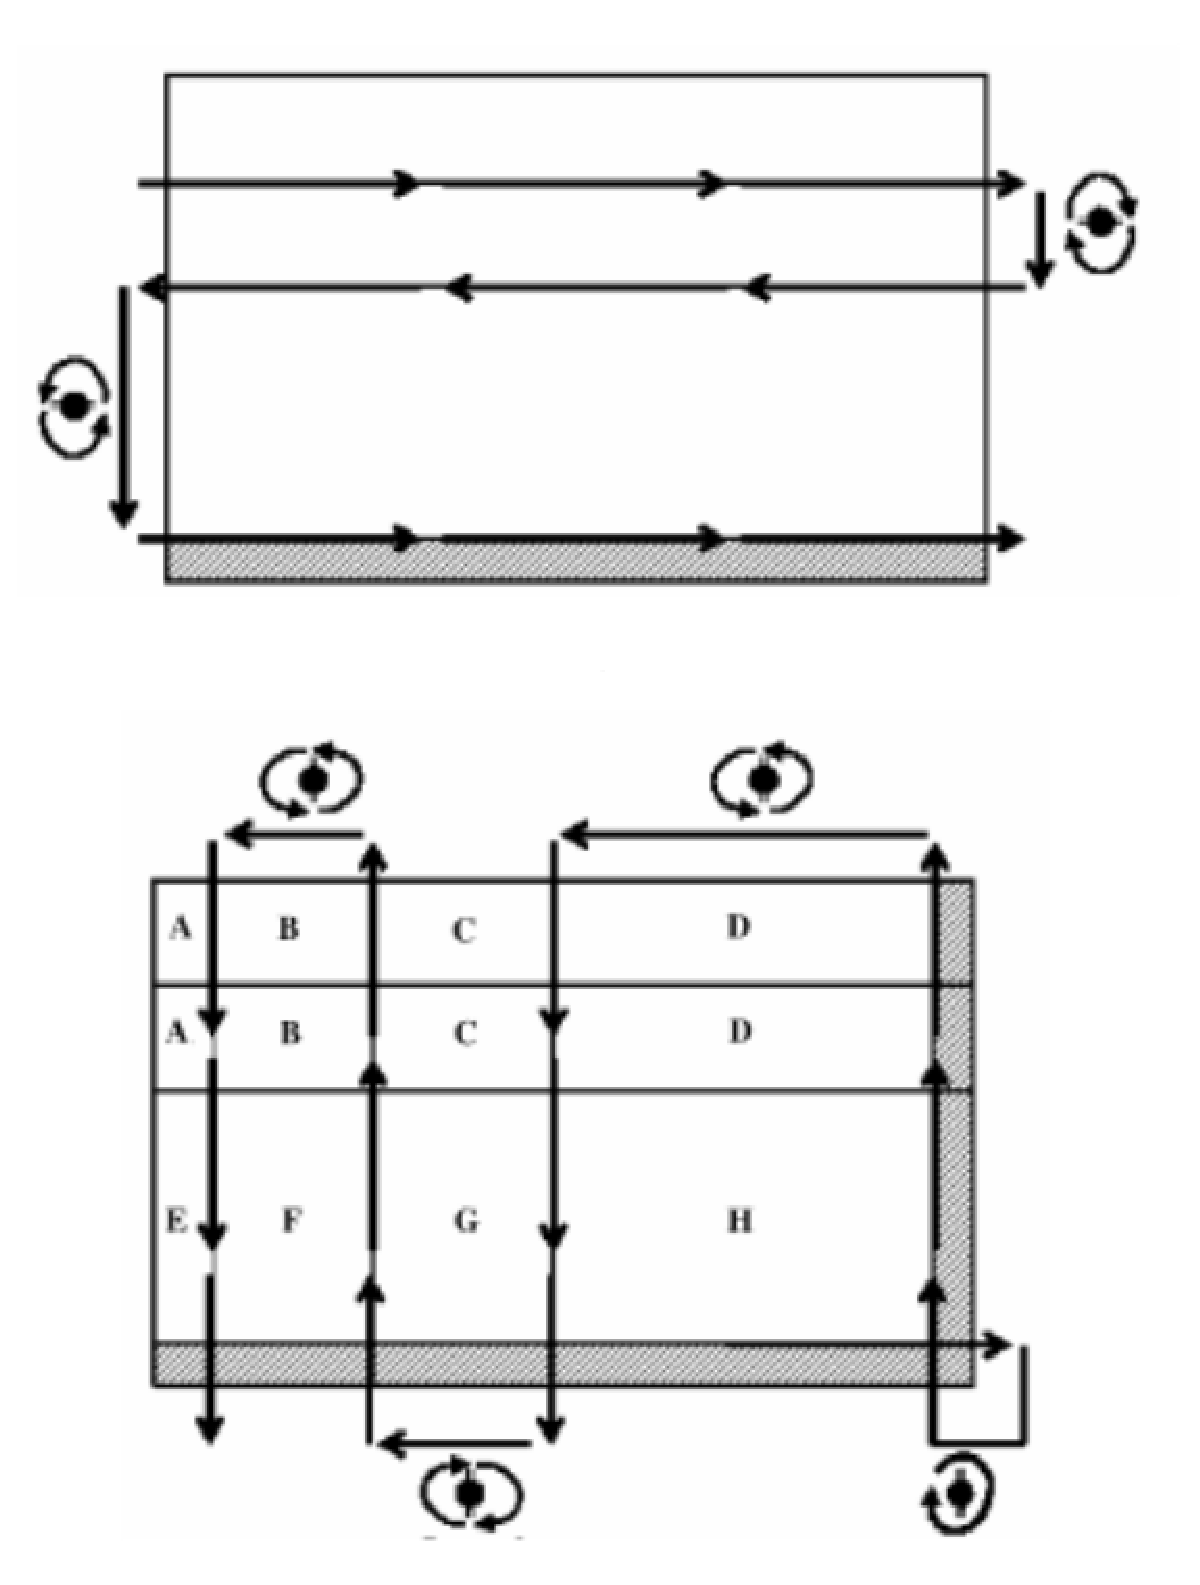
\includegraphics[width=8cm, height=10cm]{images/scacchi2.eps}
\textit{\caption{\footnotesize esempio di tagli a scacchi; prima e seconda fase}}
\end{figure}

\begin{figure}
\centering
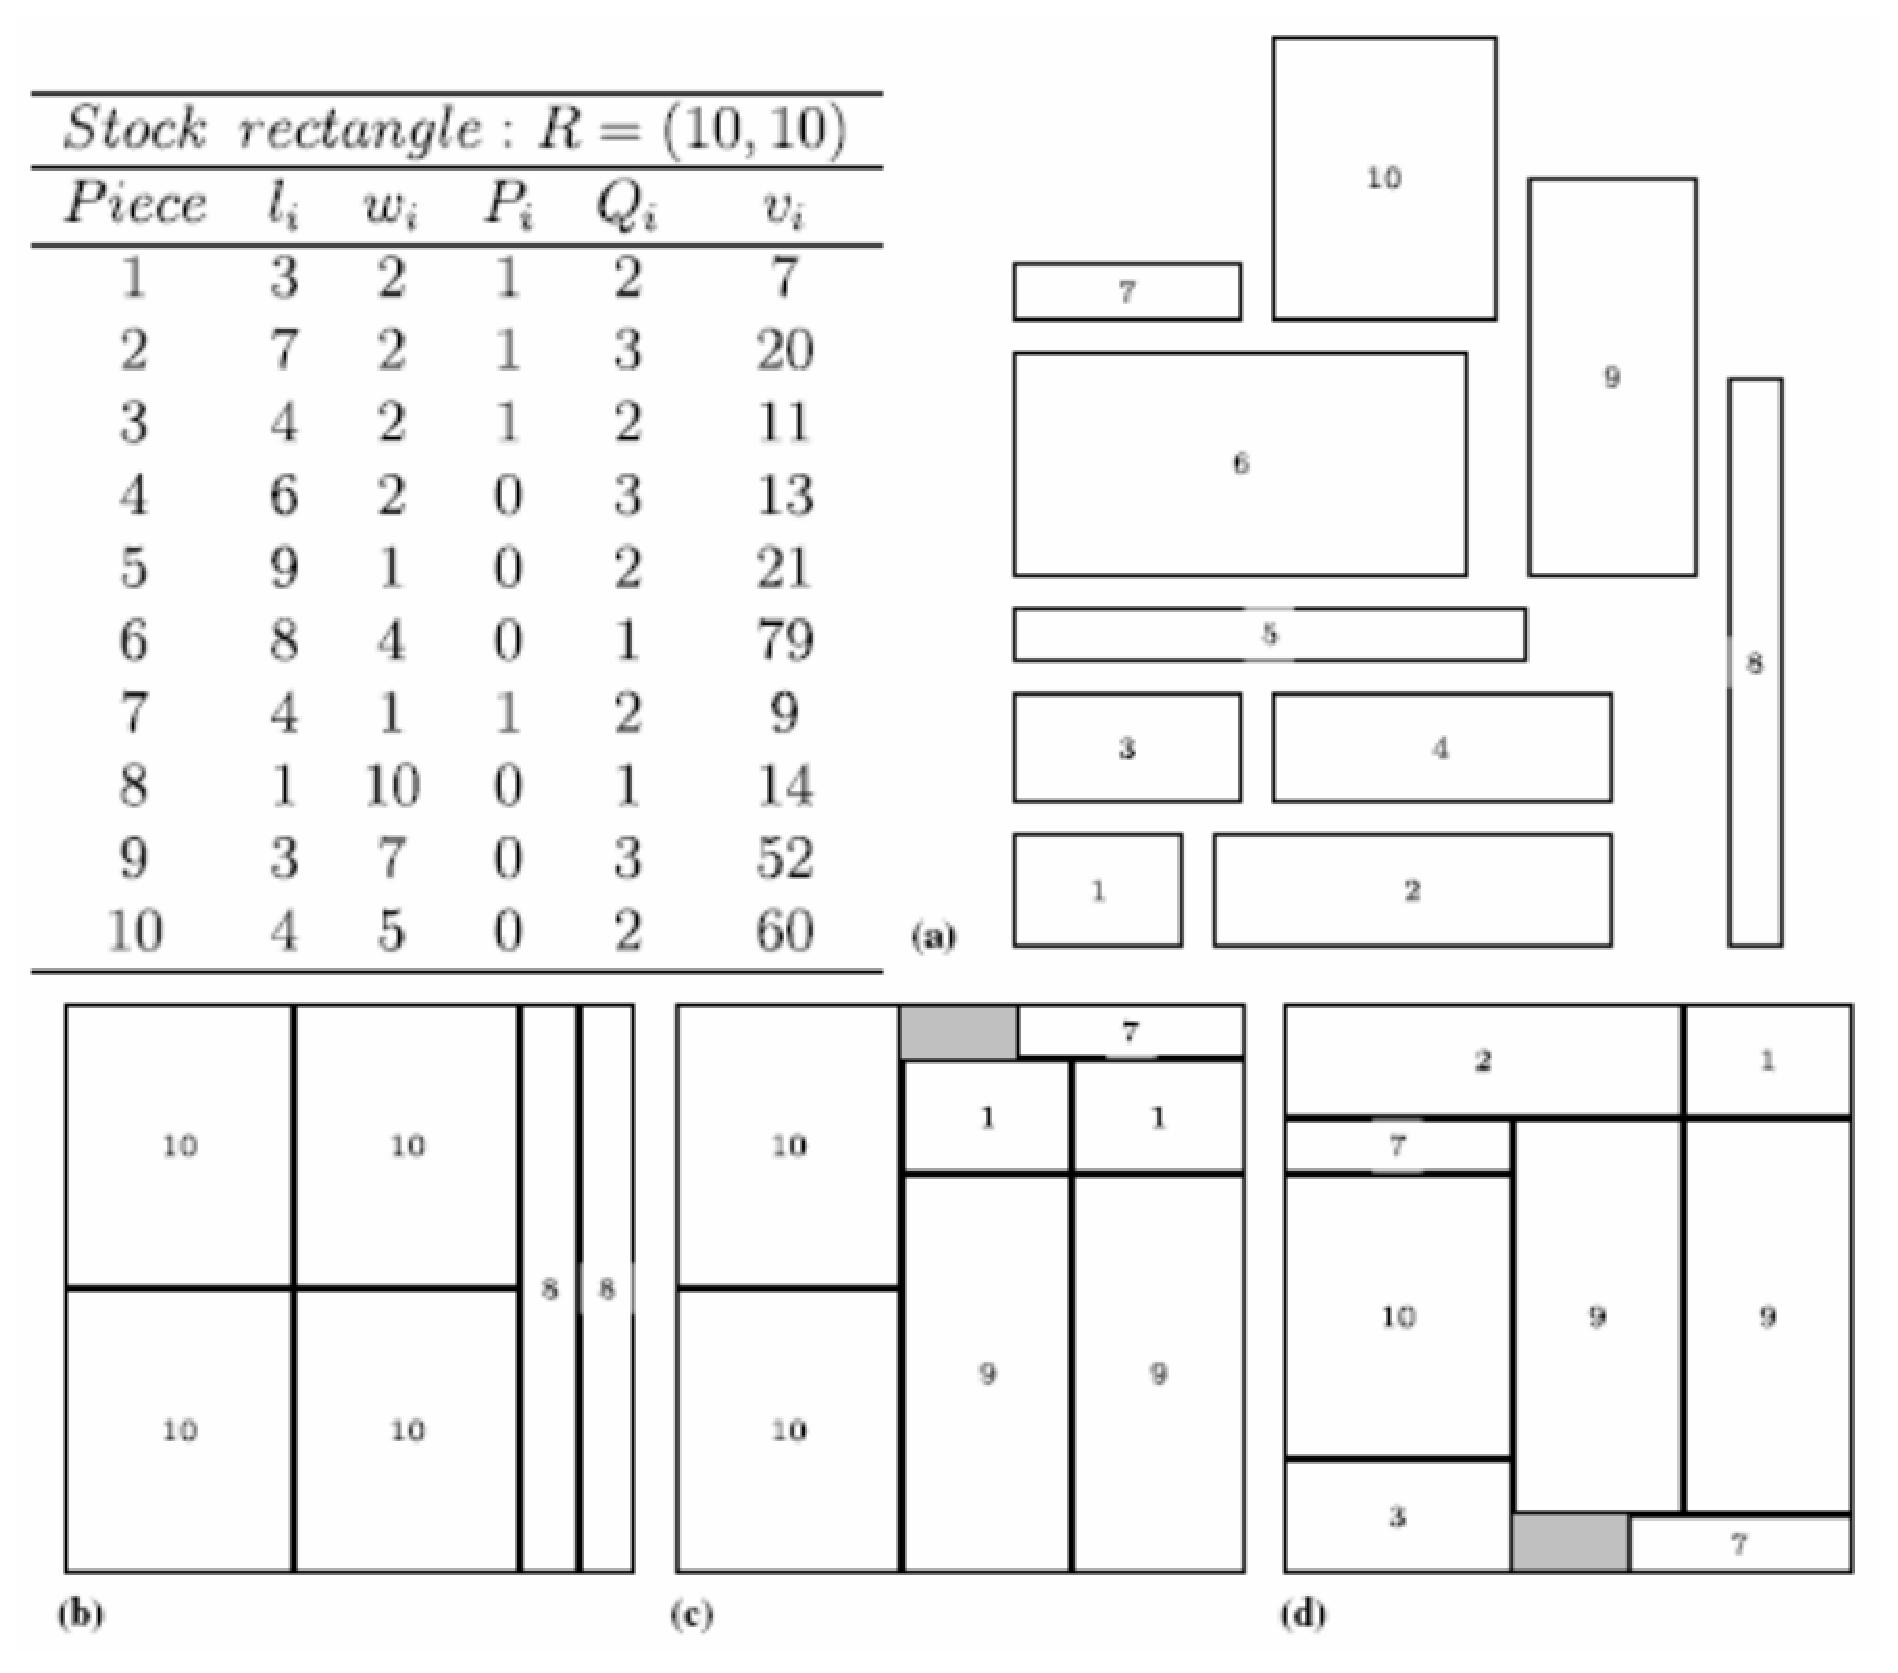
\includegraphics[width=14cm, height=12cm]{images/constrained.eps}
\textit{\caption{\footnotesize esempio di un stock di rettangoli di misura 10x10 in cui collocare i pezzi sopranumerati da 1 a 10. La figura mostra le soluzioni ottime per i problemi unconstrained (b), constrained (c) e doubly constrained (d)}}
\end{figure}

Per semplicit\`{a}, si definiranno i problemi successivi assumendo che ogni item abbia una orientazione fissa e che il vincolo del taglio a ghigliottina non sia imposto se non diversamente specificato. Inoltre ci si concentrer\`{a} sugli algoritmi cosiddetti off-line, ovvero algoritmi nei quali si ha completa conoscenza di tutti i dati in input. Gli algoritmi on-line\footnote{Sugli algoritmi on-line ci si riferisca a: J.Csirik, G.Woeginger, \textit{On-line packing and covering problems}, in: \textit{Online algorithms, Springer Lecture Notes in Computer Science}, vol. 1442, 1996, pp. 147-177
} sono invece algoritmi nei quali si impaccano gli items in ordine dell'arrivo in input (senza conoscere l'item successivo).
La descrizione del problema in modo pi\`{u} formale \`{e} la seguente: si ha un insieme di $n$ oggetti rettangolari (rectangular items) $j \in J = \left\lbrace 1,...,n \right\rbrace$, ognuno dei quali definito da una larghezza $w_{j}$ e da un'altezza $h_{j}$, e unnumero illimitato di contenitori rettangolari (\textit{bins}) aventi tutti uguale larghezza $W$ e altezza $H$.  \\
L'obiettivo, come sempre, \`{e} quello di impaccare tutti gli oggetti minimizzando il numero di contenitori. E' richiesto di sistemare gli oggetti ortogonalmente senza sovrapposizioni (il lato $w_{j}$ dell'item $j$ deve essere parallelo al lato $W$ del container).
Si assumer\`{a} inoltre, senza perdita di generalit\`{a}, che i dati di input siano interi positivi, e che $w_{j} \leq W$, $h_{j} \leq H$, con $j = (1,...,n)$.\\
Questo problema non \`{e} altro che una estensione del BPP \textit{one dimensional}, in quanto quest'ultimo \`{e} un caso speciale del BPP a due dimensioni, che compare quando $h_{j} = H$, $\forall j \in N$.\\
Il primo tentativo di costruire un modello del packing problem a due dimensioni \`{e} stato fatto da Gilmore e Gomery (1965), attraverso un' estensione del loro approccio al packing a una dimesione. Essi proposero un approccio a generazione di colonne basato sull'enumerazione di tutti i sottoinsiemi di items (patterns) che possono essere impaccati all'interno di un singolo contenitore. Sia $A_{j}$ una colonna di vettori binari di $n$ elementi $a_{ij} = (i = 1,...,n)$ che assumono valore 1 se l'item $i$ appartiene al $j-esimo$ pattern e valore 0 altrimenti.                              L'insieme di tutti i pattern accettabili viene rappresentato attraverso la matrice A, composta da tutte le possibili colonne $A_{j}$, $J = (1,...,M)$                                                                 e il corrispondente modello matematico, di tipo \textit{set partitioning}, \`{e}:
$$\mbox{minimizzare} \longrightarrow min(z) = \sum^{M}_{j=1}x_{j}$$
$$\mbox{soddisfacendo} \longrightarrow \sum^{M}_{j=1}a_{ij}x_{j} = 1 \mbox{ , } i = (1,...,n)$$ 
$$x \in \left\lbrace 0,1 \right\rbrace \mbox{ , } j = (1,...,M)$$
dove $x_{j}$ assume valore 1 se il pattern $j$ appartiene alla soluzione, 0 altrimenti.\\
Si osservi che il modello mostrato \`{e} un valido modello anche per il \textit{packing} a una dimensione, con l'unica differenza che le colonne $A_{j}$ soddisfano tutte il vincolo $\sum_{i=1}^{n}a_{ij}h_{j} \leq H$.
A causa dell'immenso numero di colonne che possono apparire in $A$, l'unico modo di affrontare il modello \`{e} quello di generare dinamicamente colonne quando ce n'\`{e} bisogno. Ma mentre per il 1BP Gilmore e Gomory sono riusciti ad avere un approccio di programmazione dinamica alla generazione di colonne, grazie all'associazione del problema a un K01, per il 2BPP essi hanno avuto difficolt\`{a} nell'associarlo al corrispondente problema a due dimensioni. Cos\`{i} essi hanno trattato il problema nel caso in cui gli oggetti devono essere impaccati in righe che formano livelli.

\subsubsection{LEVEL PACKING}
Molti degli algoritmi approssimati per il 2BPP suppongono di impaccare gli oggetti \textit{a livelli}, in cui il primo livello \`{e} costituito dal fondo del contenitore e gli oggetti sono via via impaccati appoggiando la loro base su di esso. Il livello superiore \`{e} determinato da una linea orizzontale "`"`disegnata"'"' sull'estremit\`{a} superiore dell'oggetto pi\`{u} alto del livello sottostante (figura 1.7).\\
Tre classiche strategie per l'impaccamento a livelli sono state rilevate da alcuni famosi algoritmi e in ognuno dei casi gli items sono inizialmente numerati in ordine decrescente di altezza e impaccati nella corrispondente sequenza. Se si indica con $j$ l'item corrente e con $s$ l'ultimo livello creato, le tre strategie possono essere illustrate come segue:
\begin{itemize}
\item \textbf{Next-Fit Decreasing Height (NFDH) strategy}: l'item $j$ \`{e} impaccato giustificato a sinistra al livello $s$, se ci sta. Altrimenti \`{e} creato un nuovo livello ($s:=s+1$), e $j$ viene impaccato giustificato a sinistra in esso
\item \textbf{First-Fit Decreasing Height (FFDH) strategy}: l'item $j$ \`{e} impaccato giustificato a sinistra al primo livello in cui riesce a stare, se c'\`{e}. Se nessun livello pu\`{o} contenere $j$, \`{e} creato un nuovo livello inizializzato come in NFDH
\item \textbf{Best-Fit Decreasing Height (BFDH) strategy}: l'item $j$ \`{e} impaccato giustificato a sinistra in quel livello, tra quelli dove riesce a stare, per il quale lo spazio in orizzontale inutilizzato \`{e} minimo. Se nessun livello pu\`{o} contenere $j$, \`{e} creato un nuovo livello inizializzato come in NFDH
\end{itemize} 
Nella figura 1.11 \`{e} possibile vedere le tre strategie. 
\begin{figure}[h]
\centering
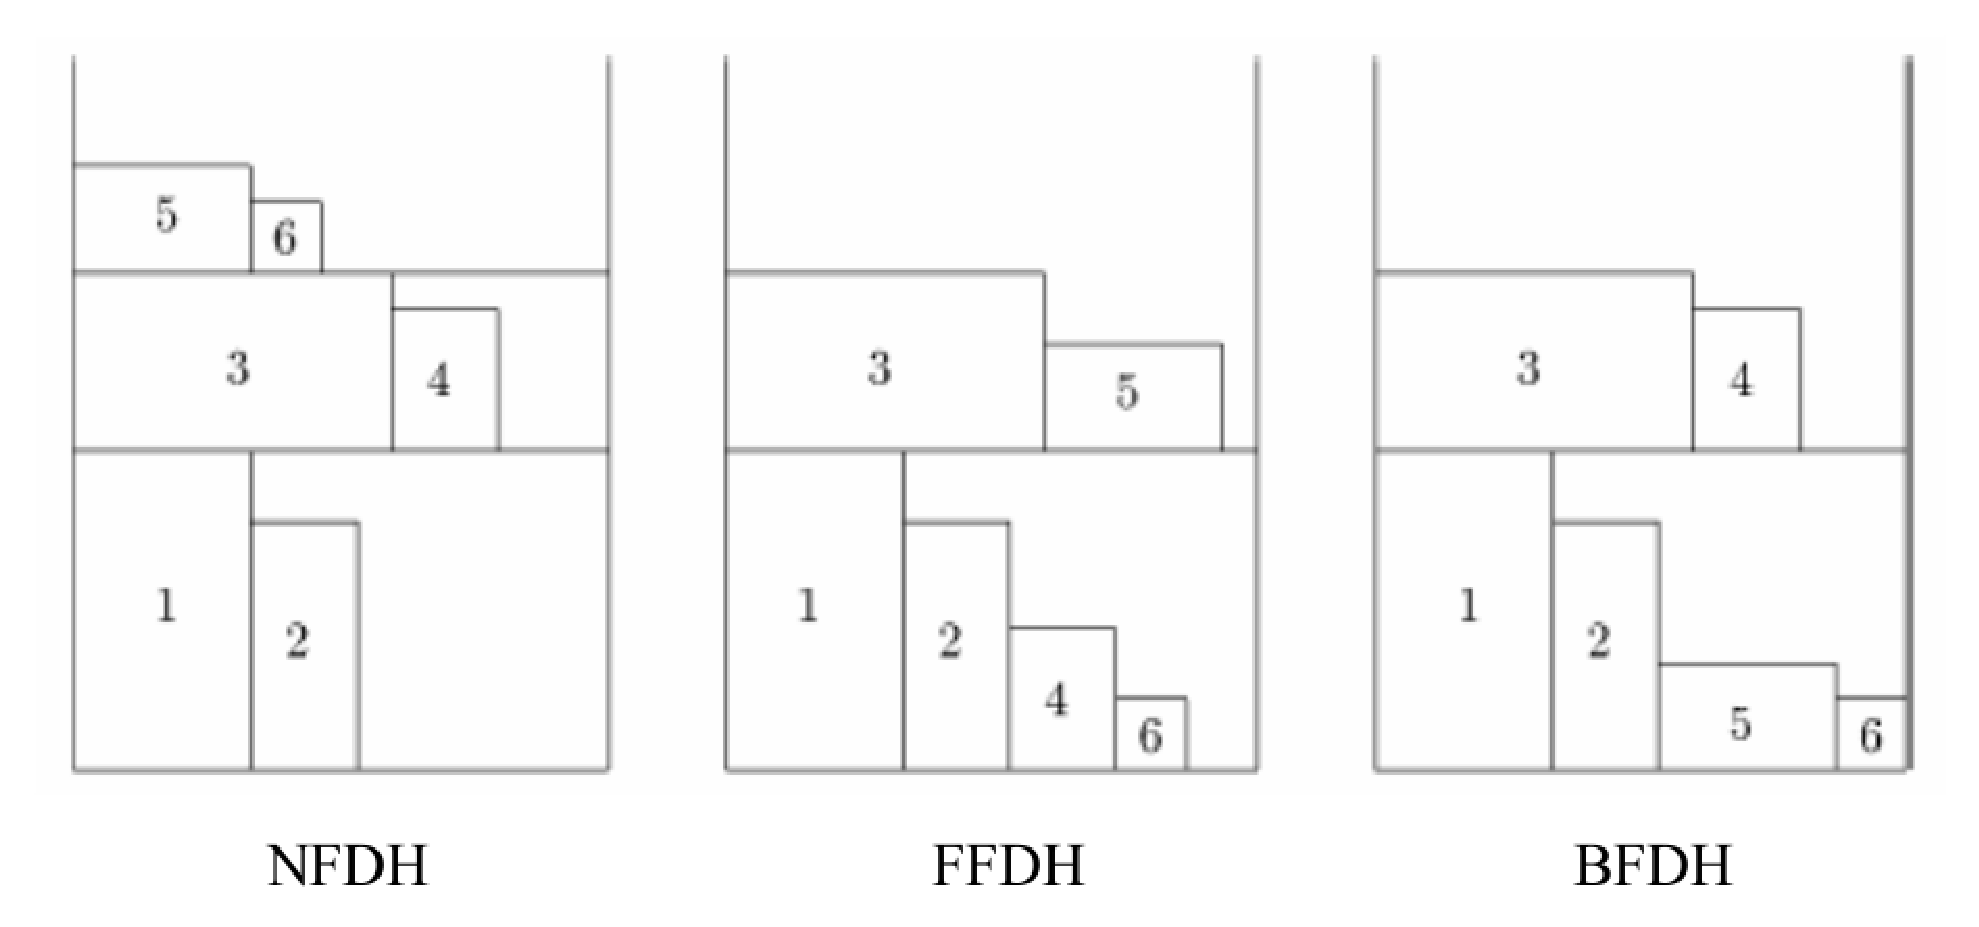
\includegraphics[width=12cm, height=6cm]{images/levelpack2.eps}
\textit{\caption{\footnotesize problemi e strategie di level packing: da sinistra a destra, NFDH, FFDH e BFDH}}
\end{figure}

\subsubsection{TWO DIMENSIONAL LEVEL BIN PACKING PROBLEM}
Indichiamo con 2LBP il problema a due dimensioni ristretto al tipo di impaccamento a livelli, supponendo, senza perdere in generalit\`{a}, che:
\begin{enumerate}
\item in ogni livello, l'oggetto a sinistra sia il pi\`{u} alto
\item in ogni contenitore, il livello pi\`{u} basso abbia maggiore altezza degli altri
\item gli oggetti siano disposti e rinumerati per valori decrescenti di $h_{j}$ (altezza dell'item $j-esimo$) 
\end{enumerate}
Si dir\`{a} che l'oggetto pi\`{u} a sinistra di un livello e il livello pi\`{u} in basso di un contenitore inizializzano il livello o il contenitore. 
\begin{figure}[h]
\centering
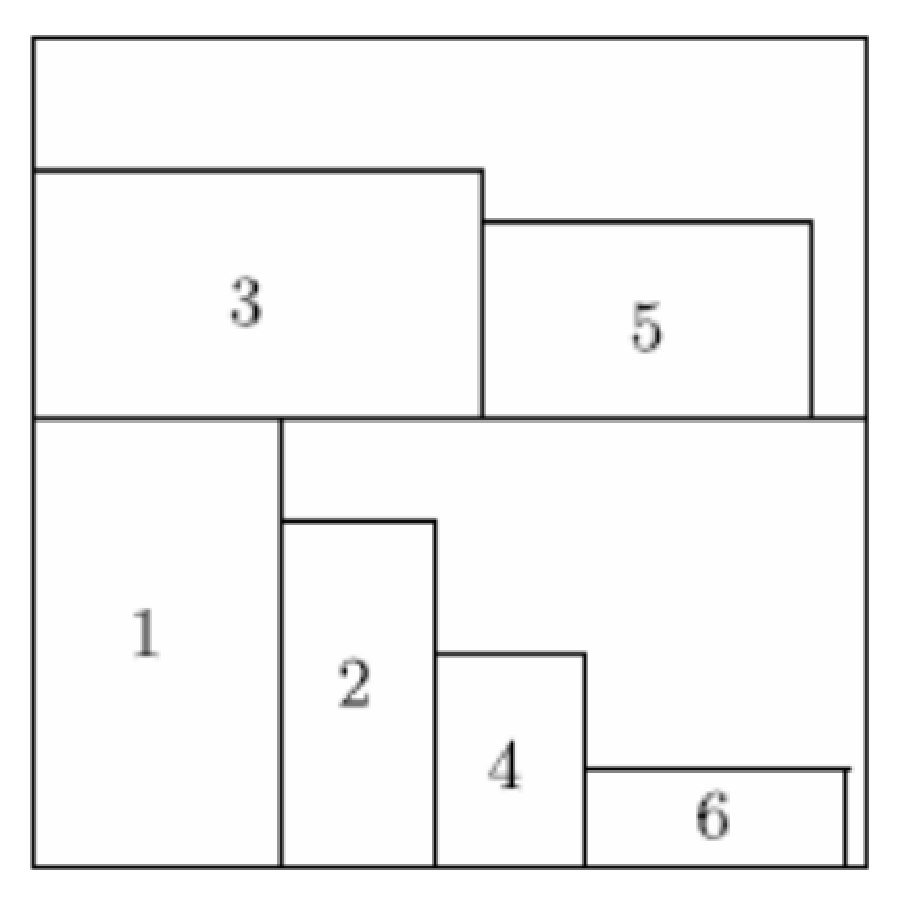
\includegraphics[width=5.5cm, height=5cm]{images/TwoLBP.eps}
\textit{\caption{\footnotesize Level packing normalizzato secondo il 2LBP}}
\end{figure}
Si pu\`{o} efficientemente costruire il modello del problema 2LBP assumendo che ci siano $n$ potenziali livelli (l'$i-esimo$ livello \`{e} associato all'item $i$ che lo inizializza), e $n$ potenziali contenitori (il $k-esimo$ contenitore \`{e} associato al potenziale $k-esimo$ livello che lo inizializza). Sia quindi $y_{i}$ , $i \in J$ una variabile binaria che assume valore 1 se l'item $i$ inizializza il livello $i$, e valore 0 viceversa. Allo stesso modo sia $q_{k}$ , $k \in J$ una variabile binaria che assume valore 1 se il livello $k$ inizializza il contenitore $k$, e valore 0 viceversa. Il modello del problema pu\`{o} essere il seguente:
\begin{equation}\label{eq13}
\mbox{min } \sum_{k=1}^{n} q_{k}
\end{equation}

\begin{equation}\label{eq14}
\mbox{suject to } \sum_{i=1}^{j-1} x_{ij}+y_{j} = 1 , \mbox{  } j = (1,...,n)
\end{equation}

\begin{equation}\label{eq15}
\sum_{j=i+1}^{n} w_{j}x_{ij} \leq (W - w_{i})y_{i} , \mbox{  } i = (1,...,n-1)
\end{equation}

\begin{equation}\label{eq16}
\sum_{k=1}^{i-1} z_{ki}+ q_{i} = y_{i} , \mbox{  } i = (1,...,n)
\end{equation}

\begin{equation}\label{eq17}
\sum_{i=k+1}^{n} h_{i}z_{ki} \leq (H - h_{k})q_{k} , \mbox{  } k = (1,...,n-1)
\end{equation}

\begin{equation}\label{eq18}
y_{i}, x_{ij}, q_{k}, z_{ki} \in \left\lbrace 0,1 \right\rbrace \mbox{ } \forall i, j, k
\end{equation}

dove $x_{ij}$, $i \in J \setminus (n)$ e $j > i$ (rispettivamente $z_{ki}$, $k \in J \setminus (n)$ e $i > k$) assume valore 1 se l'item $j$ viene impaccato a livello $i$ (rispettivamente il livello $i$ viene allocato al contenitore $k$), e valore 0 altrimenti. Inoltre:
\begin{itemize}
\item le restrizioni $j > i$ e $ i > k$ seguono dalle assunzioni 1 e 3
\item le equazioni (\ref{eq14}) e (\ref{eq16}) impongono, rispettivamente, che ogni item sia impaccato esattamente una volta, e che ogni livello usato sia assegnato a un unico contenitore
\item le equazioni (\ref{eq15}) e (\ref{eq17}) impongono, rispettivamente il vincolo di larghezza di ogni livello usato e il vincolo di altezza di ogni contenitore usato
\end{itemize}
Esperimenti computazionali hanno mostrato che il modello \`{e} abbastanza utile nella pratica. Il loro uso diretto su un risolutore commerciale di ILP produce risultati molto buoni (e, in molti casi, la soluzione ottima) per istanze realistiche con tempi di CPU brevi. Inoltre alcune varianti del problema 2LBP possono facilmente essere effettuate modificando alcuni vincoli, o aggiungendo altri vincoli lineari al modello. Il modello matematico pu\`{o} anche essere usato per produrre lower bounds, rilassando i requisiti di integralit\`{a} delle variabili.

\subsubsection{NON-LEVEL ALGORITHMS}
Oltre all'impaccamento a livelli, nella Ricerca Operativa ci sono stati altri approcci al problema di packing a due dimensioni. La principale strategia "`"`non a livelli"'"' \`{e} conosciuta come \textbf{Bottom-left} (BF), e consiste nell'impaccare l'item corrente nella posizione pi\`{u} bassa
possibile, giustificata a sinistra. Essa \`{e} stata analizzata da Baker (1980) et al., Jackobs (1996) e Liu e Teng (1999). Di questi ultimi l'algoritmo che ha conseguito risultati migliori \`{e} stato quello di Baker.
Anche Barkey e Wang (1987) hanno proposto il loro approccio BL per il caso in cui c'\`{e} un finito numero di contenitori. Il loro algoritmo \textbf{Finite Bottom-Left} (FBL) sistema gli items in ordine decrescente di larghezza. L'item corrente viene poi impaccato nella posizione pi\`{u} bassa di ogni contenitore inizializzato, giustificato a sinistra; se nessun contenitore pu\`{o} collocare l'item, ne viene inizializzato uno nuovo.
Lodi et al. (1999) hanno proposto l'\textbf{alternate directions} (AD), algoritmo che consiste nell'inizializzare L contenitori (L \`{e} il lower bound) impaccando sul loro fondo un sottoinsieme di items, seguendo una politica decrementale best-fit. Gli items rimanenti sono impaccati, in un contenitore alla volta, a strisce, alternativamente da sinistra a destra e da destra a sinistra. Non appena nessun item pu\`{o} essere impaccato in nessuna delle due direzioni, un nuovo bin inizializzato o un nuovo bin gi\`{a} parzialmente riempito diventa quello corrente. L'algoritmo ha complessit\`{a} $O(n^{3})$. Il metodo \`{e} illustrato nella figura 1.13.
\begin{figure}[h]
\centering
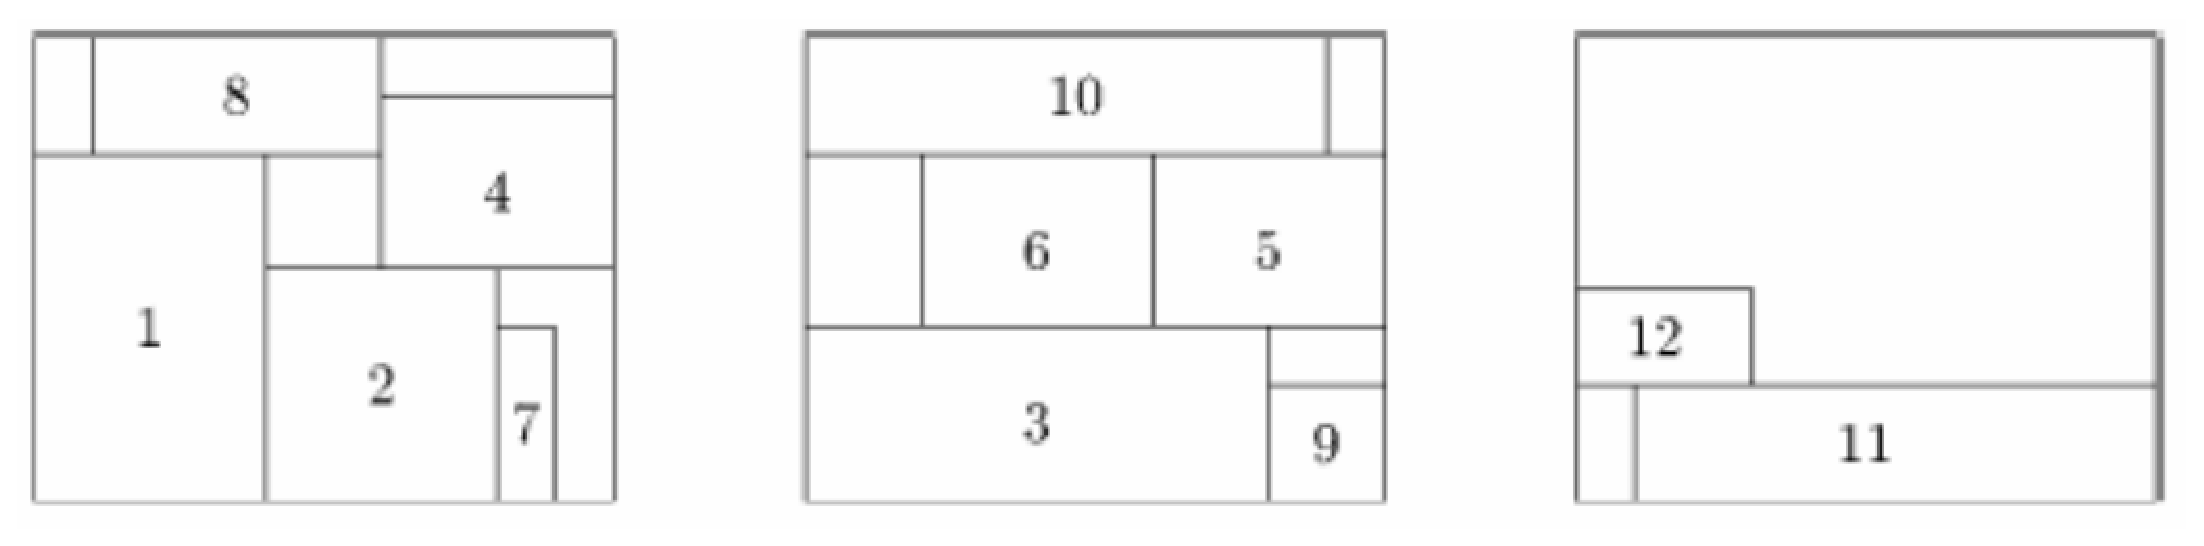
\includegraphics[width=10cm, height=3cm]{images/AD-algo.eps}
\textit{\caption{\footnotesize Algoritmo AD, Alternate Directions}}
\end{figure}\\
Beasley (1985) ha considerato il \textit{two dimensional cutting problem} nel quale ad ogni oggetto \`{e} associato un profitto, con l'obiettivo di impaccare il sottoinsieme di oggetti aventi profitto massimo in un unico contenitore (\textit{cutting stock problem}). Esso ha una formulazione ILP\footnote{Integer Linear Progamming, programmazione lineare intera: sono tutti quei problemi lineari che presentano al loro interno solo variabili intere, cio\`{e} variabili che possono assumere solo i valori contenuti all'interno del loro dominio di esistenza} basata sulla rappresentazione discreta dello spazio geometrico e l'uso delle coordinate nelle quali gli oggetti possono essere collocati, vale a dire:
$$ 
x_{ipq} =  
\left\{
\begin{array}{rl}
1 & \mbox{se l'oggetto i \`{e} posizionato con il suo angolo sinistro in (p,q)}\\
0 & \mbox{altrimenti}
\end{array}
\right.
$$
Il discorso vale per $i = 1,...,n$, $p = 0,...,W - w_{i}$ e $q = 0,...,H - h_{i}$.\\
\\Un modello simile, nel quale le coordinate $p$ e $q$ sono affrontate attraverso varibili di decisione distinte, \`{e} stato introdotto da Hadjiconstantinou e Christofides (1995). Entrambi i modelli sono usati per fornire upper bounds attraverso rilassamenti Lagrangiani e l'ottimizzazione di subgradienti.\\
\\Un approccio completamente diverso, invece, \`{e} stato recentemente proposto da Fekete e Schepers (1997), attraverso una caratterizzazione grafo-teoretica dell'impaccamento di un insieme di oggetti in un unico contenitore.
Se prendiamo in considerazione $G_{w} = (V , E_{w})$ (rispettivamente $G_{h} = (V , E_{h})$) come grafo                                                                   intervallato avente un vertice $v_{i}$ associato a ogni item $i$ nel packing e un lato tra due vertici ($v_{i}$ , $v_{j}$) se e solo se le proiezioni degli items $i$ e $j$ sull'asse orizzontale (rispettivamente sul verticale) si sovrappongono. E' stato dimostrato appunto da Fekete e Schepers che se il packing \`{e} accettabile allora:
\begin{itemize}
\item per ogni insieme $S$ di solidi di $G_{w}$ (rispettivamente di $G_{h}$) si ha che $E_{v_{i} \in S} w_{i} \leq W$ (rispettivamente $E_{v_{i} \in S} h_{i} \leq H$)
\item $E_{w} \bigcap E_{h} = \left\lbrace \right\rbrace$
\end{itemize}
 
\begin{figure}[h]
\centering
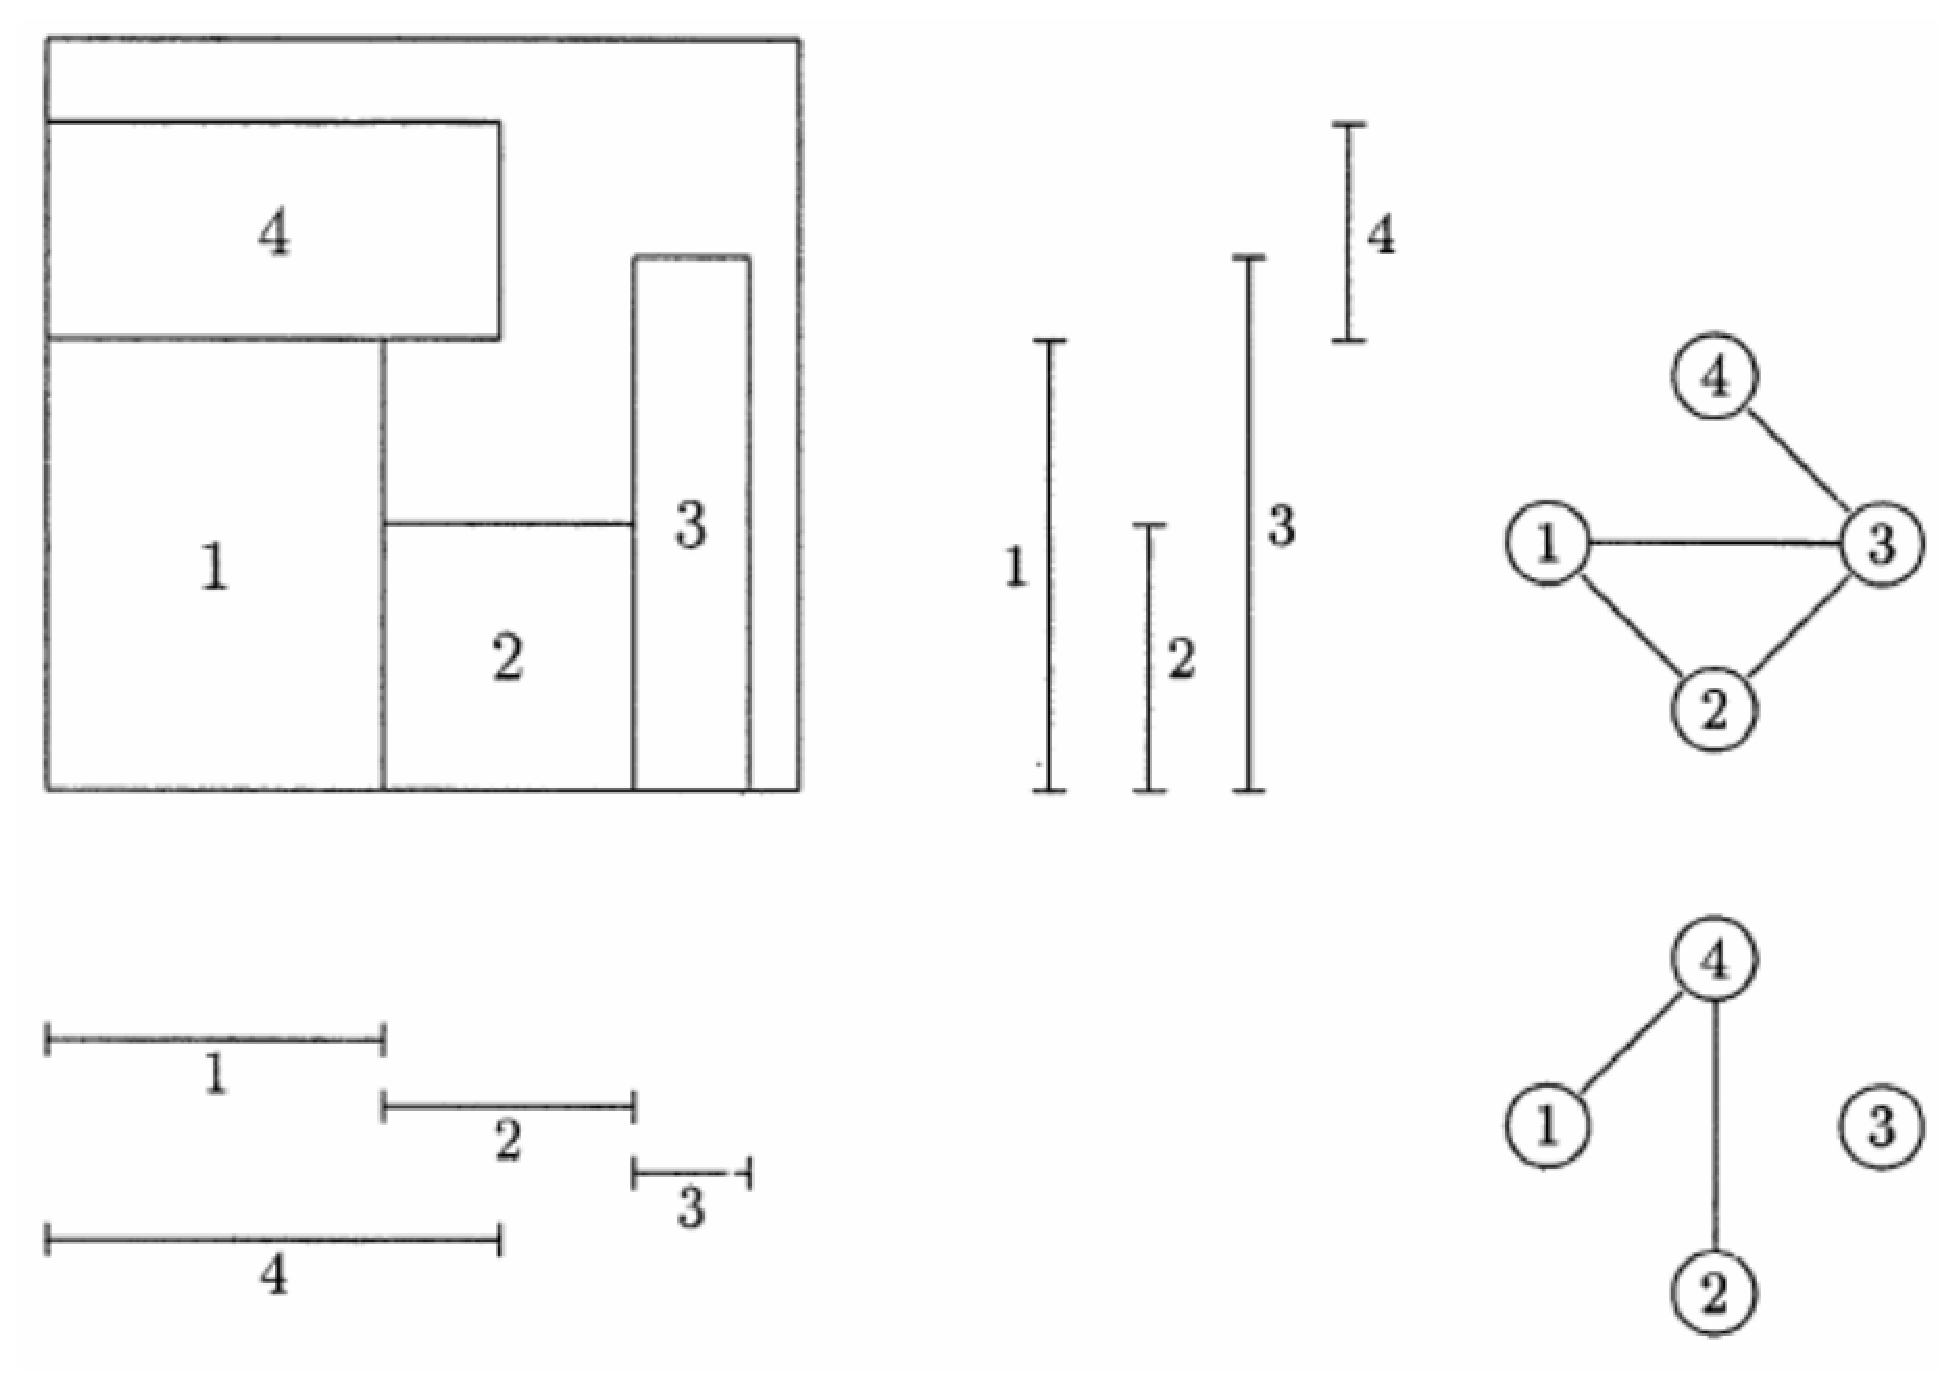
\includegraphics[width=10cm, height=7cm]{images/FS-algo.eps}
\textit{\caption{\footnotesize Algoritmo di Fekete e Schepers}}
\end{figure}

\subsubsection{ALGORITMI METAEURISTICI}
L'\textbf{euristica}\footnote{di derivazione greca, rappresenta una parte dell'epistemologia e del metodo scientifico} \`{e} un metodo di approccio alla soluzione dei problemi che non segue un chiaro percorso, ma si affida all'intuito e allo stato temporaneo delle circostanze, al fine di generare nuova conoscenza. \`{E} opposto al procedimento algoritmico e quindi, in ambito informatico, si definisce euristico il lavoro di un software che non opera meccanicamente, ma utilizza invece una tecnica virtualmente creativa, cio\`{e} non si limita ad analizzare i dati secondo confronto di dati noti, ma prova a simularne il comportamento\footnote{tra i pi\`{u} diffusi software di questo tipo, troviamo gli antivirus e le applicazioni contro il \textit{phishing} per cui \`{e} fondamentale affidarsi a tecniche non consuete, come invece lo \`{e} l'analisi per confronto}.\\
Nel settore della Ricerca Operativa, quindi pi\`{u} in generale dove si fondono informatica e matematica, si utilizzano algoritmi euristici come particolari tipi di procedimenti le cui soluzioni non rispecchiano la soluzione ottima per quel dato problema. 
L'euristica \`{e} un approccio di risoluzione dei problemi molto diffuso nella \textit{simulazione} per vari possibili motivi:
\begin{itemize}
\item la risoluzione del problema ottimo pu\`{o} essere impossibile
\item la risoluzione del problema ottimo pu\`{o} essere troppo costoso in termini di tempo o di capacit\`{a} di elaborazione
\end{itemize}
Le tecniche metauristiche sono oggi un frequente strumento usato per trovare la soluzione approssimata dei problemi di ottimizzazione combinatoria. Dowsland (1993) present\`{o} uno dei primi approcci metauristici al 2BPP. Il suo algoritmo \textit{simulated annealing}\footnote{processo che mira a trovare un minimo globale quando si \`{e} in presenza di pi\`{u} minimi locali. deriva dalla scienza dei metalli, dov'\`{e} usato per descrivere il processo di eliminazione di difetti reticolari dai cristalli tramite una procedura di riscaldamento seguita da un lento raffreddamento (molto usato in Microelettronica). Nel nostro caso un difetto reticolare corrisponde ad una combinazione errata di due oggetti.} esplora sia le soluzioni accettabili che le soluzioni nelle quali gli items si sovrappongono. Durante la ricerca, la funzione obiettivo consiste perci\`{o} nell'eliminazione totale delle aree sovrapposte, e il vicinato contiene tutte le soluzioni corrispondenti allo spostamento verticale o orizzontale degli items. Appena una nuova soluzione migliore di quella corrente viene trovata, l'upper bound \`{e} fissato alla sua altezza.\\
\\Un'estensione dell'approccio di Dowsland al 2BP \`{e} stato proposto da Faero et al. (1999). Essi usano un simile vicinato e una simile strategia di ricerca all'interno di un approccio \textit{guided local search}. Dato un lower bound e un upper bound sul valore della soluzione ottima, se questi non coincidono, l'algoritmo assegna casualmente gli items impaccati nel contenitore di indice pi\`{u} alto ad altri contenitori. La nuova soluzione \`{e} di solito non ammissibile, cos\`{i} la nuova funzione obiettivo risulta essere la totale eliminazione delle aree sovrapposte, pi\`{u} un termine che penalizza, durante la ricerca, i modelli inammissibili. Il vicinato \`{e} esplorato attraverso gli spostamenti degli items. Minimizzare la nuova funzione obiettivo corrisponde a trovare una soluzione ammissibile che coinvolge un contenitore in meno. Il processo \`{e} iterato fino a quando l'upper bound non eguaglia il lower bound, oppure fino a quando non si raggiunge un limite di tempo prefissato. Speciali tecniche per ridurre la complessit\`{a} computazionale per l'esplorazione di questo grande vicinato sono state implementate.\\
\\Lodi et al. (1999) hanno sviluppato un algoritmo \textit{tabu search} per il 2BPP. La caratteristica principale di quest'ultimo \`{e} l'adozione di uno schema di ricerca e un vicinato che sono indipendenti dallo specifico packing problem da risolvere. La struttura pu\`{o} anche essere usata per ogni variante del 2BPP ed \`{e} stata facilmente estesa anche al problema a tre dimensioni. Partendo da una soluzione accettabile, le mosse la modificano, attraverso un euristico costruttivo, cambiando l'impaccamento di un sottoinsieme $S$ di items al momento impaccati in $k$ diversi contenitori, e cercando di riempire uno specificato target bin (un contenitore che pu\`{o} essere facilmente riempito). Sia $S_{i}$ l'insieme degli items momentaneamente impaccati nel contenitore $i$: il target bin $t$ \`{e} quello che minimizza, tra tutti i bins $i$, la funzione:
$$ \varphi (S_{i}) = \alpha \dfrac{\sum_{j \in S_{i}} w_{j}h_{j} } {WH} - \dfrac{\vert S_{i} \vert}{n}$$
($\alpha$ rappresenta un peso positivo pre-stabilito).
Tale formula fornisce appunto la misura della facilit\`{a} con cui un contenitore pu\`{o} essere riempito. Una volta selezionato il target bin, il sottoinsieme $S$ \`{e} definito in modo da includere un item $j$, nel target bin e gli oggetti contenuti attualmente dagli altri $k$ bins. Il nuovo packing per $S$ \`{e} ottenuto eseguendo un appropriato algoritmo euristico A su $S$. Il valore di $k$, che definisce la dimensione e la struttura del vicinato corrente, \`{e} automaticamente aggiornato durante la ricerca in modo da evadere dall'ottimo locale. Se la mossa impacca gli items $S$ in $k$ (o meno) contenitori, cio\`{e} l'item $j$ \`{e} stato rimosso dal target bin, un nuovo item \`{e} stato selezionato, un nuovo insieme $S$ \`{e} definito, e una nuova mossa \`{e} stata eseguita. Altrimenti $S$ \`{e} cambiato selezionando un diverso insieme di $k$ bins, o un diverso item $j$ dal target bin (se tutte le possibili configurazioni di $k$ bins sono state provate per il corrente item $j$). Se l'algoritmo si blocca, cio\`{e} il target bin non \`{e} riempito, il vicinato si allarga aumentando il valore di $k$ fino a un limite superiore prefissato. C'\`{e} una \textit{tabu list} e un \textit{tabu tenure} per ogni valore di $k$. Un alto valore di $k$ implica una potente ricombinazione, ma anche l'evidente inconveniente di un elevato tempo computazionale per l'esplorazione del vicinato. L'unica parte che dipende dallo specifico problema \`{e} l'euristico costruttivo, usato per ottenere la prima soluzione e per ricombinare gli items ad ogni mossa.

\subsubsection{ALGORITMI ESATTI}
Martello e Vigo (1998) hanno proposto un algoritmo esatto per il 2BPP. Gli items sono inizialmente sistemati in ordine decrescente rispetto alla loro area, e una procedura di riduzione prova a determinare il packing ottimale di alcuni contenitori, riducendo quindi la dimensione dell'istanza. La prima soluzione in carica, di valore $z^{*}$, \`{e} poi ottenuta euristicamente. L'algoritmo si basa su uno schema \textit{two-level branching}:
\begin{itemize}
\item \textit{outer branch-decision tree}: a ogni nodo decisionale, un item \`{e} assegnato a un contenitore senza specificare la sua posizione attuale
\item \textit{inner brach-decision tree}: \`{e} determinato un packing accettabile (se esiste) per gli items assegnati momentaneamente a un contenitore euristicamente o attraverso un algoritmo che enumera tutti i possibili modelli
\end{itemize}
L'outer branch-decision tree \`{e} ricercato in un modo detto \textit{depth-first}, facendo uso di lower bound. Quando \`{e} possibile stabilire che ulteriori items non ancora assegnati possono essere messi in un dato contenitore inizializzato, questo bin viene chiuso: un bin inizializzato e non chiuso \`{e} chiamato \textit{active}. Al livello $k \mbox{ }( k = 1, ..., n)$, l'item k \`{e} assegnato, a turno, a tutti i contenitori inizializzati e, possibilmente, ad un nuovo bin (se il numero di bins richiesto dalla soluzione parziale corrente \`{e} minore di $z^{*} - 1$). L'accettabilit\`{a} dell'assegnamento di un item $k$ a un contenitore gi\`{a} contenente un insieme $I$ di items \`{e} controllata euristicamente. Un lower bound $L(I)$ \`{e} calcolato per l'istanza $I$ definita dagli items correntemente assegnati al contenitore: se $L(I)>1$ segue un \textit{backtracking}. Altrimenti, sono applicati a $I$ algoritmi euristici: se un single-bin packing accettabile viene trovato, si riprende l'enumerazione. Se non lo si trova, lo schema \textit{inner branching} elenca tutti i possibili modi di impaccare gli items $I$ in un unico bin attraverso il principio \textit{left-most downward}: ad ogni livello, l'item successivo viene posizionato, a turno, in tutte le posizioni dove esso ha il lato sinistro adiacente al lato destro di un altro item o al lato sinistro del contenitore, e il lato inferiore adiacente al lato superiore di un altro item o al lato inferiore del contenitore. Non appena si trova un packing accettabile per tutti gli items $I$, si riprende l'enumerazione. Se un tale packing non esiste, si esegue un \textit{outer backtracking}.

\subsubsection{ULTIME VERSIONI E APPLICAZIONI}
I packing problems a due dimensioni continuano a essere studiati. Ultimamente riveste particolare importanza l'articolo riguardante il \textit{two-dimensional orthogonal packing probelm}, redatto da Clautiaux, Carlier e Moukrim (2006). Essi propongono procedure di riduzione e un nuovo metodo esatto soprannominato TSBP (\textit{two-step bin packing}). Il metodo riduce sostanzialmente il numero di nodi visitati del metodo di Martello e Vigo (1998). Questo pu\`{o} essere spiegato per il fatto che per molte istanze non ammissibili, il problema rilassato non ha soluzioni. Inoltre essi propongono metodi per risolvere parte delle ridondanze che ricorrono nel metodo \textbf{branch \& bound} e nuovi lower bounds che possono essere usati con risultati positivi.\\
\\Sempre Clautiaux, Carlier e Moukrim, riferendosi al bin packing problem con aggiunta di varianti hanno presentato un nuovo articolo (che compare su Operations Research Letters) in cui propongono un nuovo metodo esatto per il problema. Esso si basa su una decomposizione iterativa dell'insieme di items all'interno di due disgiunti sottoinsiemi. L'algoritmo, confrontato con alcuni benchmarcks della letteratura conferma l'efficienza del metodo.\\
\\Interessante anche l'articolo di Cui e Zhang (2006) sull'\textit{unconstrained two-dimensional cutting problem of rectangular pieces}. Esso descrive un nuovo algoritmo \textit{two-stage}, ovvero come tagliare generici blocchi in due fasi, con altre due o pi\`{u} fasi richieste per tagliare i blocchi in pezzi: in un primo momento tagli verticali dividono il foglio di materiale in segmenti, poi tagli orizzontali dividono i segmenti in blocchi. Un generico blocco contiene generiche striscie, e ogni taglio su un blocco produce una di queste striscie. L'algoritmo presentato ricorre a una programmazione dinamica per determinare il layout delle striscie per ogni blocco, risolve un problema di tipo knapsack per ottenere il layout dei blocchi su ogni segmento e il layout del segmento su ogni foglio di materiale. I risultati computazionali indicano che l'algoritmo \`{e} molto efficiente e ha tempi di esecuzione ragionabili.\\
\\Solo un anno fa inoltre alcuni ricercatori dell'universit\`{a} della Danimarca (Pisinger, Sigurd, 2005) hanno pubblicato un articolo sul packing a due dimensioni considerando due nuove variabili: il cosiddetto \textit{two-dimensional variable sized bin packing problem} (2DVSBPP) \`{e} il problema di impaccare un insieme di items in un insieme di bins rettangolari aventi diverse misure e diversi costi, e l'obiettivo \`{e} quello di minimizzare il costo dei contenitori usati per impaccare gli oggetti. Nello scritto uscito lo scorso anno su Discrete Optimization gli autori presentano una formulazione intera lineare del problema e introducono diversi lower bound. In esso \`{e} inoltre sviluppato un algoritmo esatto basato sul \textit{branch-and-price}.

\subsection{Two Dimensional Strip-packing Problem}
Questo tipo di problema ha come scopo quello di allocare ortogonalmente tutti gli item su di una striscia (assolutamente senza alcuna sovrapposizione) minimizzando l'altezza totale occupata dal packing. Il problema in questione \`{e} di tipo NP-hard e quindi la ricerca ha improntato gran parte delle soluzioni basandosi su algoritmi approssimati, i quali si avvicinano molto alla soluzione ottima, ma non garantiscono l'ottimizzazione completa su tutti gli insiemi di dati proposti. Il \textit{two dimensional strip-packing problem} (2SPP) pu\`{o} essere visto come la trasformazione del problema di \textit{bin packing} a una dimensione, dove quest'ultimo ha soluzione "`"`facile"'"'. Partendo infatti da una qualsivoglia istanza del 1BPP si ottiene facilmente un'istanza del 2SPP aggiungendo al problema una variabile $h_{j} = 1$ per $j \in J$: il valore della soluzione ottima di tale istanza \`{e} ottima anche per l'istanza del 1BPP. \\
Tale problema compare in diversi contesti reali, come nel taglio di rulli di carta o di tessuto, nel taglio di legno, metallo o vetro da pezzi si stocks standardizzati, nell'allocazione di memoria nei computer, per elencare solo alcuni degli usi pi\`{u} comuni.
\begin{figure}[h]
\centering
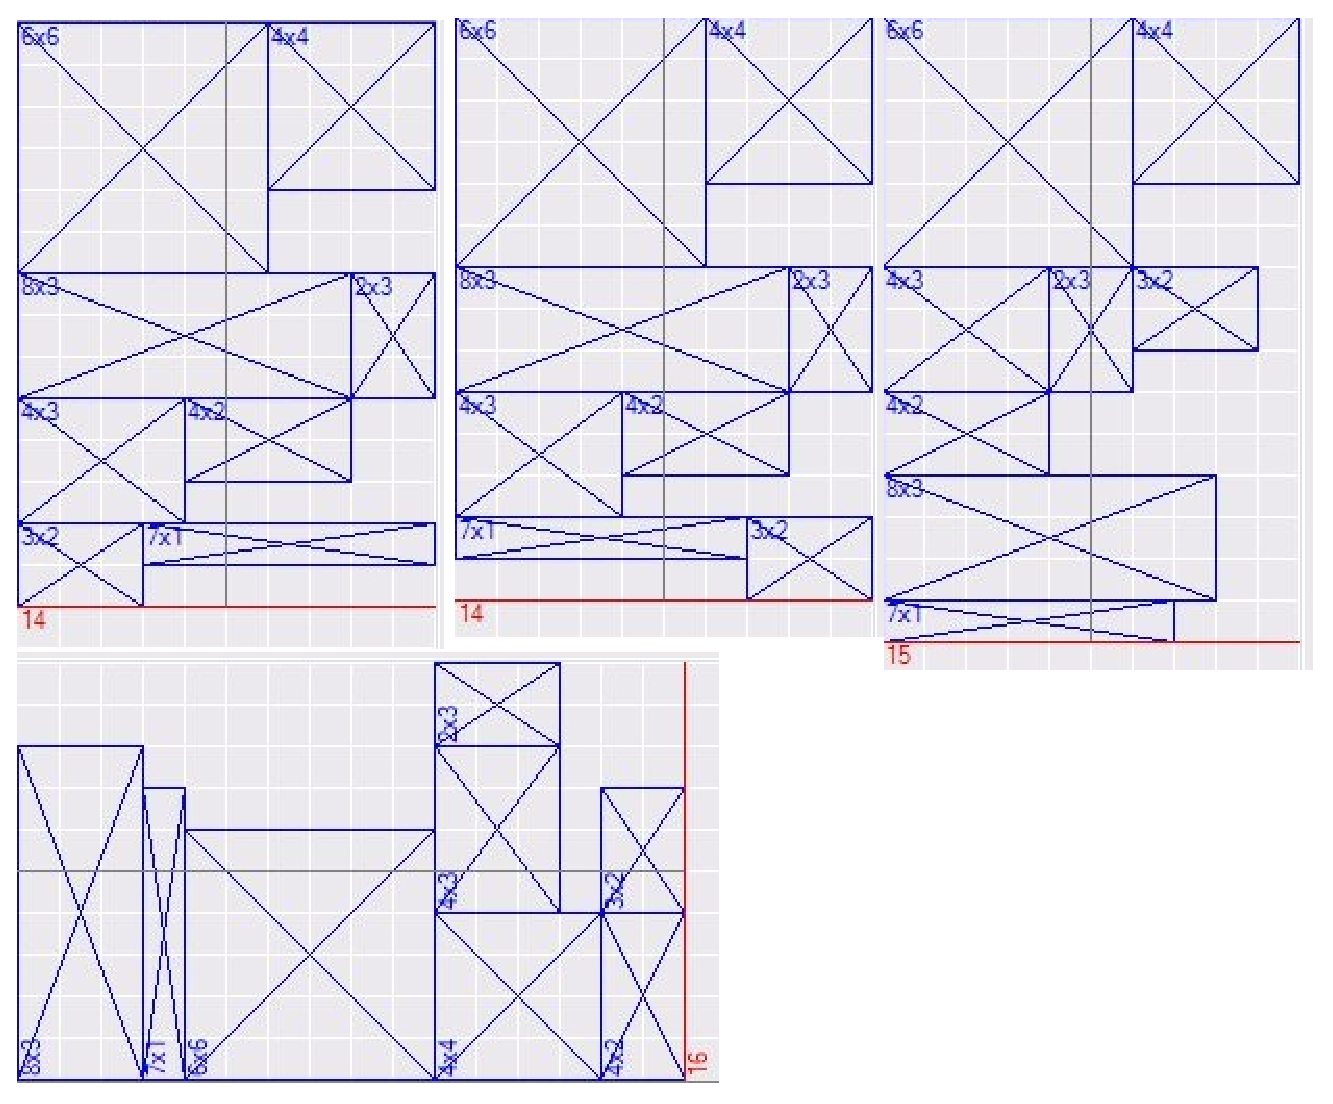
\includegraphics[width=9cm, height=9cm]{images/2spp.eps}
\textit{\caption{\footnotesize alcune soluzioni al 2SPP basate sull'euristica two dimensional variable sized bin packing problem (2DVSBPP)}}
\end{figure}

\subsubsection{ALGORITMI ESATTI}
Il miglior algoritmo esatto del problema \`{e} stato presentato da Martello, Monaci e Vigo (2003). In esso si assume che gli items abbiano un'orientazione fissa, ovvero che non possano essere ruotati. Si suppone inoltre che tutti i dati in input siano positivi interi, e che $w_{j} \leq W ( j = 1, ..., n)$. Per determinare la soluzione esatta del 2SPP, sono stati inseriti particolari lower bounds (ottenuti alcuni da semplici considerazioni geometriche, altri da un nuovo rilassamento del problema) in un  "`"`adattamento"'"' dell'algoritmo branch-and-bound proposto da Scheithauer (1997) e Martello et al. (2003) per riempire un unico contenitore bidimensionale. L'albero decisionale funziona in questo modo: ad ogni nodo decisionale, la potenziale soluzione corrente, che impacca gli items di un sottoinsieme $I \subset J$, \`{e} incrementato selezionando a turno ogni item $j \in J \setminus I$, e generando nodi discendenti allocando $j$ in tutte le sue posizioni ammissibili. \`{E} stato provato in Martello et al. (2000) che gli items di I definiscono un "`"`involucro"'"' che separa le due regioni dove gli items $J \setminus I$ possono o no essere posizionati, e ci\`{o} \`{e} sufficiente per generare nodi corrispondenti al piazzamento dell'angolo inferiore sinistro di $j$ nei punti dove la pendenza dell'involucro cambia da verticale a orizzontale. Questi sono chiamati \textit{corner points} e possono essere determinati in un tempo $O(|I| \log |I|)$:
\begin{figure}[h]
\centering
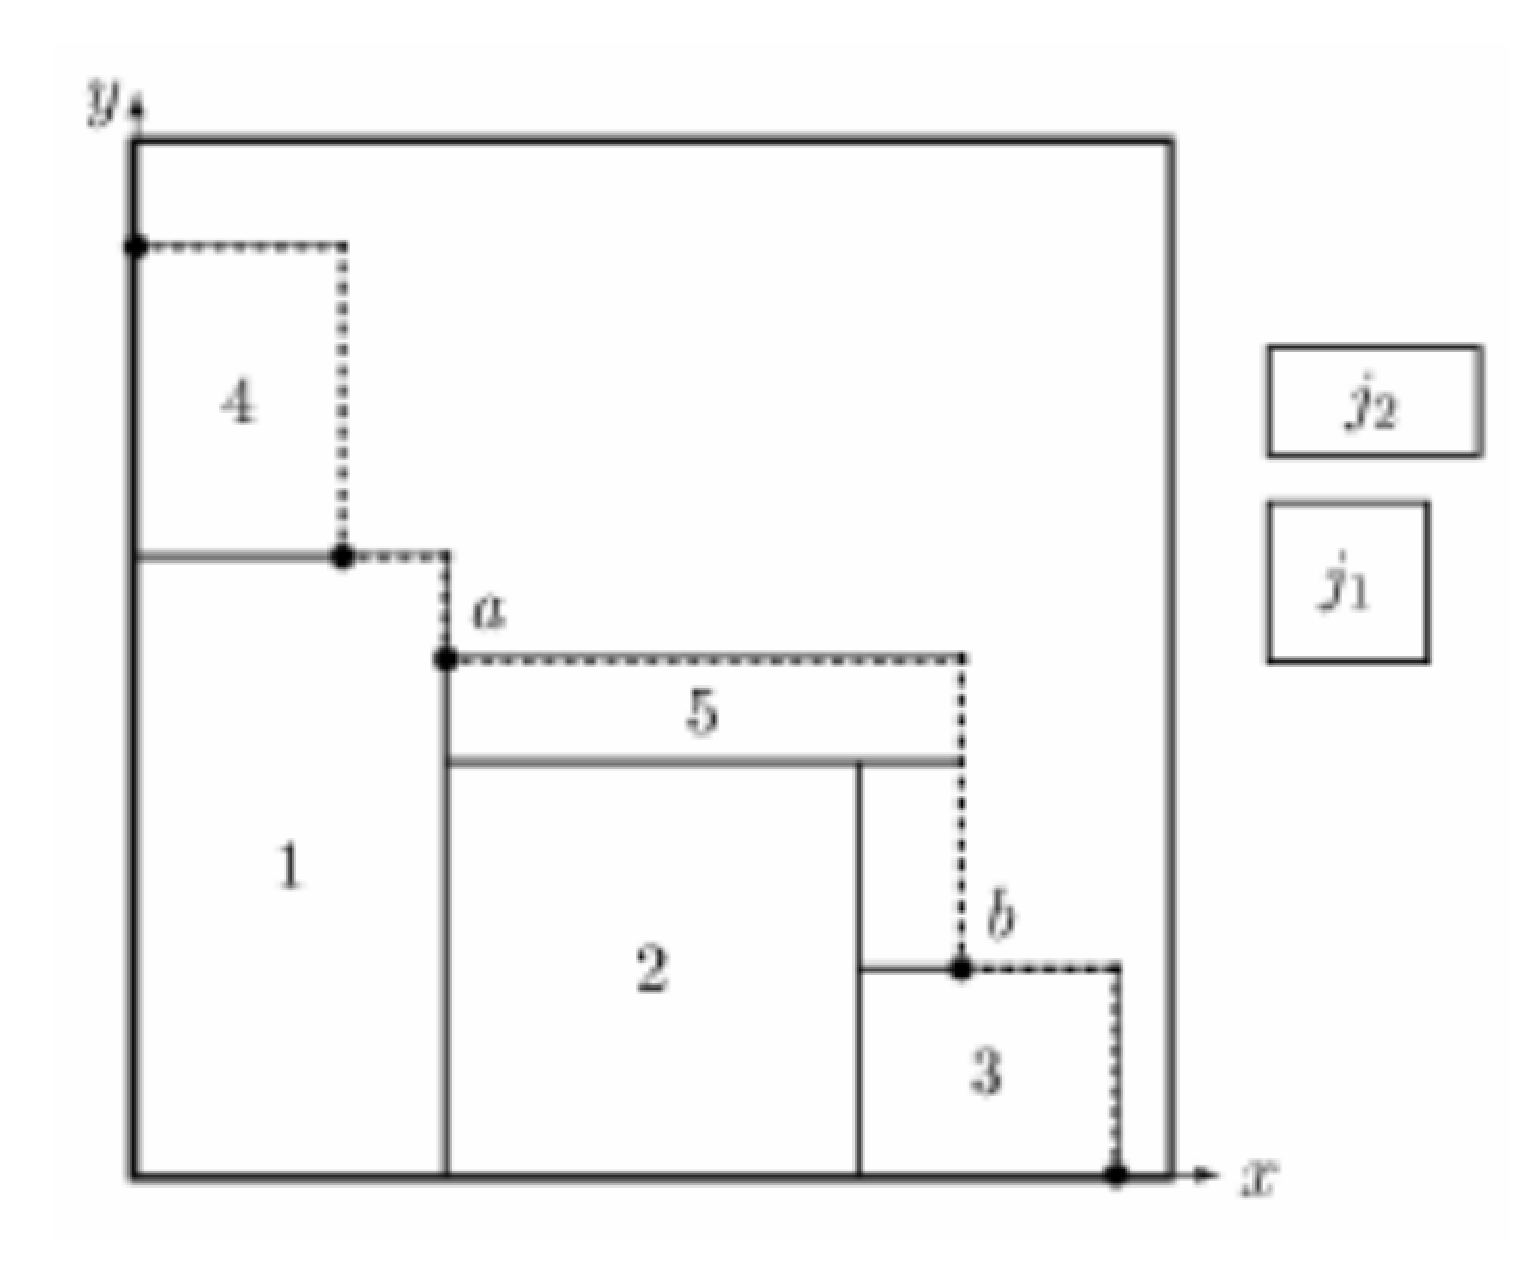
\includegraphics[width=8.4cm, height=7cm]{images/corner.eps}
\textit{\caption{\footnotesize involucro associato agli items di $I = \left\lbrace 1,2,3,4,5 \right\rbrace$ dove i corner points sono indicati con un puntino nero.}}
\end{figure}
Lo schema branch-and-bound \`{e} stato poi migliorato in due modi: attraverso una tecnica per evitare la generazione multipla di nodi decisionali che producono lo stesso modello, e attraverso l'aggiunta di efficaci algoritmi di approssimazione. Si considerino, ad un dato livello $k$ dell'albero decisionale, due punti d'angolo $a, b$ e due items $j_{1} , j_{2} \in J \setminus I$: la regola di base potrebbe generare quattro nodi, corrispondenti a quattro coppie di tipo (corner point, item): ($a, j_{1}$), ($a, j_{2}$), ($b, j_{1}$), ($b, j_{2}$), dove la coppia indica il nodo. Tra i figli di ($a, j_{1}$) si pu\`{o} poi generare un nodo corrispondente alla coppia ($b, j_{2}$), e, allo stesso livello $k+1$, si pu\`{o} generare, tra i figli di ($b, j_{2}$), un identico nodo corrispondente a ($a, j_{1}$). Per evitare situazioni di questo genere, che non si presentano solo tra i figli, ma anche, pi\`{u} generalmente, tra discendenti di nodi fratelli, Martello et al. hanno adottato la seguente tecnica. Per ogni potenziale nodo, corrispondente al piazzamento di un item $j$ in un angolo $a$, essi determinano gli involucri che si dovrebbero generare dall'insieme di item $\left\lbrace j \right\rbrace \cup (I \setminus \left\lbrace i \right\rbrace), \forall i \in I$. Se esiste un item $i \in I$, correntemente piazzato, in un corner point $b$, per il quale l'involucro corrispondente a $\left\lbrace j \right\rbrace \cup (I \setminus \left\lbrace i \right\rbrace)$ include $b$ tra i suoi punti d'angolo, sappiamo che il corrente nodo potenziale potrebbe produrre un modello identico a quello prodotto cambiando l'ordine nel quale $i$ e $j$ sono considerati nel processo di branching. Ecco perch\'{e} il nodo \`{e} generato solo se $j > i$.
Per trovare una buona soluzione iniziale ammissibile per il nodo padre, o per migliorare la solizione corrente per i nodi discendenti, sono implementati alcuni classici algoritmi euristici della letteratura (Coffman et al. (1980); Baker et al. (1980)...).
\begin{figure}[h]
\centering
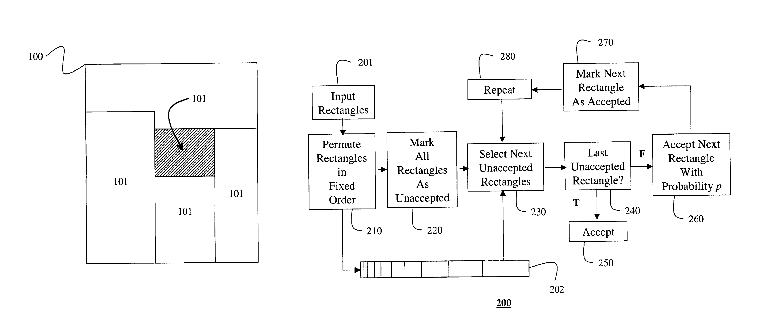
\includegraphics[width=15cm, height=7cm]{images/spp.eps}
\textit{\caption{\footnotesize illustrazione schematica e molto sommaria del processo strip-packing}}
\end{figure}

\subsubsection{ALGORITMI METAEURISTICI}
Un approccio metauristico interessante \`{e} quello presentato da Iori, Martello e Monaci (2003). Il 2SPP viene risolto attraverso una combinazione tra un algoritmo \textit{tabu search} e un algoritmo di tipo genetico\footnote{metodo euristico di ricerca ed ottimizzazione, ispirato al principio della selezione naturale di Charles Darwin che regola l'evoluzione biologica. Gli algoritmi genetici sono applicabili alla risoluzione di un'ampia variet\`{a} di problemi d'ottimizzazione non indicati per gli algoritmi classici, compresi quelli in cui la funzione obiettivo \`{e} discontinua, non derivabile, stocastica, o fortemente non lineare.}. L'algoritmo di tipo tabu search di riferimento \`{e} l'algoritmo 2BP-TS proposto da Lodi, Martello e Vigo (1999) eseguito indicando con $z^{*}$ il valore della soluzione corrente del 2SPP, inizialmente calcolata attraverso algoritmi BUILD\footnote{algoritmo che parte dalla soluzione del rilassamento del 1CBP e costruisce una
soluzione ammissibile per il 2SPP congiungendo i tagli per ricostruire l'item di origine. Si veda a proposito: \textit{Martello, Monaci e Vigo: An exact approach to the Strip-Packing problem}} e $TP_{2SP}$\footnote{inizializza la striscia ad una lunghezza L, e considera gli items a seconda dell'ordine in cui vengono dati. Per poi impaccarli secondo un preciso metodo. A riguardo si proprone: \textit{Iori, Martello, Monaci: Metaheuristic Algorithms for the Strip Packing Problem}}, e applicando particolari procedure di post-ottimizzazione descritte dagli autori. L'algoritmo genetico \`{e} invece un algoritmo sviluppato dagli stessi e indicato con 2SP-GA. Esso si basa sulla permutazione della struttura dei dati che rappresenta l'ordine nel quale gli items sono impaccati nella striscia. La dimensione della popolazione \`{e} costante ma vengono prodotti nuovi individui attraverso criteri di riproduzione. \`{E} inoltre ottenuta una diversificazione attraverso l'immigrazione e la mutazione. La ricerca \`{e} inoltre intensificata attraverso ricerca locale. Infine nell'algoritmo, viene considerata la storia dell'evoluzione, in modo da intensificare la ricerca in aree promettenti, e da evitarla nei minimi locali.\\
Sui due algoritmi metauristici sono stati effettuati vari esperimenti computazionali sia su istanze prese dalla letteratura sia su istanze create casualmente: sia il 2SP-TS che il 2SP-GA hanno mostrato un buon comportamento empirico. In particolare si \`{e} potuto notare come l'approccio genetico abbia migliori prestazioni nel caso di istanze di piccole dimensioni e con piccoli valori della misura $W$ della striscia da riempire, mentre l'opposto accade per l'altro algoritmo. Tuttavia le performance migliori sono state ottenute sperimentando l'\textit{hybrid algorithm}, ovvero la combinazione dei due algoritmi sopra citati.\\
\\Oltre al metodo sopra menzionato, nella tabella 1.1 (al termine del capitolo) \`{e} riportato un elenco di alcuni di altri recenti sviluppi metauristici per il 2SPP.  In particolare in essa sono stati distinti:
\begin{itemize}
\item quattro sottotipi di \textit{strip packing problem}:
\begin{itemize}
\item RF $\rightarrow$ i pezzi possono essere ruotati di $90^{\circ}$ ma non sono richiesti tagli a ghigliottina
\item RG $\rightarrow$ i pezzi possono essere ruotati di $90^{\circ}$ e sono richiesti tagli a ghigliottina
\item OF $\rightarrow$ l'orientamento dei pezzi \`{e} fisso ma non sono richiesti tagli a ghigliottina
\item OG $\rightarrow$ l'orientamento dei pezzi \`{e} fisso e sono richiesti tagli a ghigliottina
\end{itemize}
\item tre gruppi di approccio alla soluzione dei metauristici (Hopper e Turton, 2000/2001):
\begin{enumerate}
\item Il metodo del primo gruppo usa una codifica delle soluzioni. Di solito, una soluzione genera una sequenza di piazzamenti per i pezzi. La ricerca viene svolta dal relativo euristico nello spazio delle soluzioni e tipicamente usa operatori indipendenti dal problema
\item Gli approcci per le soluzioni del secondo gruppo sono in una posizione intermedia. Mentre, da un lato, soluzioni codificate, contengono gi\`{a} informazioni geometriche o di layout, \`{e} richiesto un procedimento addizionale di piazzamento per il posizionamento finale. Tipici di questo gruppo \`{e} una codifica specifica al problema di riferimento, spesso basata su grafi
\item L'approccio del gruppo $3$ non usa la codifica. La ricerca avviene direttamente nello spazio dei layout completamente definiti, che sono poi manipolati come detto da specifici operatori
\end{enumerate}
\item tre tipi di algoritmi metaeuristici:
\begin{itemize}
\item GA $\rightarrow$ genethic algorithms
\item SA $\rightarrow$ simulated annealing
\item TS $\rightarrow$ tabu search
\end{itemize}
\end{itemize}

\begin{table}[t]
\begin{center}
\begin{tabular}{|||p{3.5cm}||*{2}{c|}| c |||}
\hline
\textbf{Authors, source} & \textbf{SPP subtype} & \textbf{Approaches} & \textbf{Methaeuristics} \\
\hline
\hline
\bfseries    Jacobs (1996) & RF &  1 & GA  \\
\hline
\bfseries    Dagli and Poshyanonda (1996, 2004) & RF &  1 & GA  \\
\hline
\bfseries    Liu and Teng (1999) & RF &  1 & GA  \\
\hline
\bfseries    Hopper and Turton (2000) & RF &  1 & GA  \\
\hline
\bfseries    Hopper and Turton (2000) & RF &  1 & SA  \\
\hline
\bfseries    Hopper and Turton (2000) & RF &  1 & NE$\star$  \\
\hline
\bfseries    Mumford, Valenzuela et al. (2003) & RG &  1 & GA  \\
\hline
\bfseries    Kr$\ddot{o}$ger (1993, 1995) & RG &  2 & Parallel GA  \\
\hline
\bfseries    Schnecker (1996) & RG &  2 & Parallel GA  \\
\hline
\bfseries    Ratanapan and Dagli (1997, 1998) & RF &  3 & GA  \\
\hline
\bfseries    Iori et al. (2002) and Monaci (2001) & OF &  Hybrid & Hybrid GA+TS  \\
\hline
\hline
\end{tabular}
\end{center}
\caption{Algoritmi metaeuristici per il 2SPP con pezzi rettangolari; $\star$ indica NaiveEvolution, ovvero un GA con mutazione ma senza crossover}
\label{lab:table}
\end{table}

\subsubsection{LEVEL PACKING}
Anche per il \textit{two dimensional strip packing problem} come per il BPP esiste un packing a livelli, proposto da Lodi, Martello e Monaci (2002). Tale alternativa consiste nel modificare la funzione obiettivo eliminando tutti i vincoli e le varibili relativi al bin packing problem visto 
precedentemente, in modo da ottenere il modello seguente:
$$\mbox{minimizzare} \longrightarrow \mbox{min } \sum^{n}_{i=1}h_{i}y_{i}$$
$$\mbox{soddisfacendo} \longrightarrow \sum^{j-1}_{i=1}x_{ij} + y_{j} = 1, \mbox{ } j = \left\lbrace 1,...,n \right\rbrace ,$$ 
$$\sum_{j=i+1}^{n} w_{j}x_{ij} \leq (W - w_{j})y_{i}, \mbox{ } i \in N = \left\lbrace 1,...,n-1 \right\rbrace$$ 
$$y_{i}, x_{ij} \in  \left\lbrace 0,1 \right\rbrace \mbox{ } \forall i,j$$

\subsection{Two Dimensional Knapsack Problem}
Consideriamo innanzitutto un problema knapsack di tipo rettangolare\footnote{d'ora in poi chiameremo tale problema un \textit{rectangle packing problem}}, ossia un problema a due dimensioni avente come \textit{items} degli oggetti rettangolari. \\ Sono dati: un insieme di $N = (1,...,n)$ piccoli rettangoli (gli items), in cui ognuno ha una larghezza $w_{j}$, un'altezza $h_{j}$ e un profitto $p_{j}$ con $j \in N$ e un contenitore di larghezza $W$ e altezza $H$. L'obiettivo consiste, analogamente agli altri casi precedenti, nell'inserire nel container (knapsack) un sottoinsieme di items che massimizzi il profitto; il vincolo \`{e} che gli oggetti non si sovrappongano e che ognuno di essi abbia il lato $h_{j}$ parallelo al lato $H$ del contenitore\footnote{si definisce con questi vincoli un tipo di problema denominto \textit{orthogonal packing problem without rotation}}. Si noti che 2KP \`{e} una generalizzazione del gi\`{a} citato \textit{1-dimensional
Knapsack problem}, visto come caso particolare avente $h_{j} = H \mbox{  } \forall j \in N$.\\
Anche il \textit{two-dimensional Knapsack Problem} (2KP) \`{e} un problema NP-hard e in letteratura sono stati studiati molti metodi per risolverlo, a partire dal fondamentale studio di Gilmore e Gomory (1965). Tuttavia, sembra non essere conosciuto nessun algoritmo approssimato che garantisca una \textit{worst-case performance}; ci\`{o} \`{e} sorprendente dato che alcuni risultati di questo genere sono invece noti per il connesso problema di impaccamento a due dimensioni.
Procediamo illustrando un naturale rilassamento del 2KP:
$$max \mbox{ } \sum_{j \in N}p_{j} x_{j}$$
$$\sum_{j \in N}(w_{j}h_{j})x_{j} \leq WH$$ 
$$x \in \left\lbrace 0,1 \right\rbrace, (j \in N)$$
nel quale ogni item $j, ( j \in N )$ ha un profitto $p_{j}$ e peso $w_{j}h_{j}$, uguale all'area del rettangolo $j$ nel 2KP, e capacit\`{a} del contenitore $WH$, uguale all'area del contenitore nel 2KP. Per una istanza $I$ del 2KP, sia $OPT(I)$ la soluzione ottima e $U_{KP}( I )$ l'upper bound su $OPT(I)$ corrispondente alla soluzione ottima della formulazione sopra descritta. Il rapporto di performance peggiore \`{e} definito come:
$$ r(U_{KP}) \doteq \stackrel{inf}{I} \left\lbrace \dfrac{OPT(I)}{U_{KP}(I)} \right\rbrace $$
Il worst-case ratio trovato finora \`{e} $r(U_{KP}) = \frac{1}{3}$. Tale rilassamento, approfondito da Caprara e Monaci (2003) costituisce una buona base di partenza per quattro nuovi algoritmi per risolvere il 2KP: essi rappresentano l'approccio esatto al problema pi\`{u} recente.\\
Oltre a Caprara e Monaci (2003), altri studi sono stati condotti a riguardo:\\
\\
\underline{Beasley}\\
Basley (2003) ha presentato un algoritmo euristico di tipo genetico per la risoluzione del problema; \`{e} basato su una nuova e non lineare formulazione del problema ed \`{e} rappresentato da una popolazione euristica (\textit{Population heuristics}, PH) dove la popolazione delle soluzioni al problema si evolve progressivamente. La nuova PH proposta si discosta dalle "`"`semplici"'"' popolazioni euristiche precedenti e pu\`{o} essere sintetizzata nel seguente modo:
\begin{enumerate}
\item si genera una popolazione iniziale
\item si valuta il fitness e l'unfitness degli individui (repeat)
\item si selezionano due individui genitori della popolazione (random)
\item si ricombinano i genitori producendo un solo figlio, attraverso il crossover
\item si muta il figlio; uno ogni dieci figli viene mutato
\item si valuta il fitness e l'unfitness del figlio e miglioralo usando uno schema euristico di miglioramento
\item si sostituisce un membro della popolazione con il figlio usando uno schema di rimpiazzamento, a meno che il figlio non sia un duplicato di un membro della popolazione, in tale caso lo si scarta
\item ci si ferma dopo aver riportato la miglior soluzione incontrata\\
\end{enumerate}
\underline{Hadjiconstantinou and Christofides}\\
Hadjiconstantinou e Christofides (1995) hanno presentato una procedura esatta \textit{tree-search}\footnote{ricerca ad albero} per risolvere il kanpsack a due dimensioni. Essi hanno considerato il caso in cui c'\`{e} un numero massimo di volte in cui un pezzo pu\`{o} essere usato. L'algoritmo limita la dimensione del \textit{tree} usando un bound derivante da un rilassamento lagrangiano della formulazione binaria del problema. Un'ottimizzazione del subgradiente viene poi usata per ottimizzare il bound. Le performance computazionali dell'algoritmo indicano che la precedente \`{e} una  procedura veramente capace di risolvere ottimamente il problema nel caso di medie dimensioni.\\
\\
\underline{R.Alvarez-Valdes, F.Parrenho, J.M.Tamarit}\\
Tali ricercatori presentano nel 2006 un algoritmo tabu search completo di mosse basate sulla riduzione e l'inserzione di pezzi, di procedure di intensificazione e diversificazione basate su una memoria a lungo termine. In particolare l'efficienza delle mosse \`{e} basata su una strategia \textit{merge and fill}. 
\begin{figure}[h]
\centering
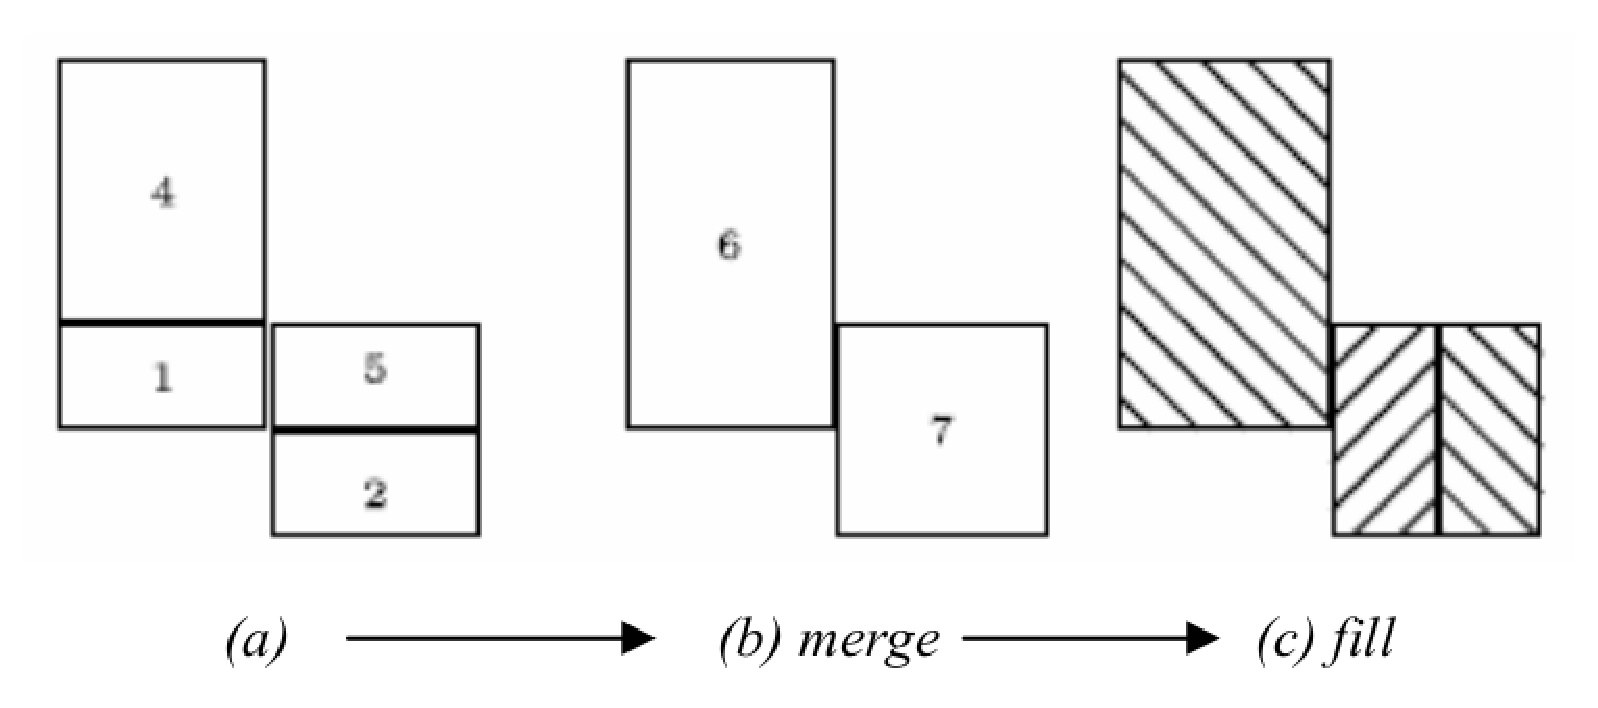
\includegraphics[width=10cm, height=5cm]{images/mergeandfill.eps}
\textit{\caption{\footnotesize strategia Merge and Fill}}
\end{figure}
\\I risultati computazionali mostrano che tutte queste idee funzionano bene in particolare per i problemi \textit{constrained} e \textit{doubly constrained}.\\
\\
\underline{Hadjiconstantinou, Iori}\\
Presentano un nuovo approccio euristico per risolvere il problema, semplice ma molto efficiente: nella fase preliminare, vengono calcolati semplici upper bounds e soluzioni iniziali sono ottenute attraverso \textit{greedy algorithms}. In seguito \`{e} eseguita una ricerca genetica, che usa la selezione dei genitori, la teoria etilista, l'immigrazione, e diversi operatori crossover. L'approccio genetico diviene ibrido dopo aver usato un euristico on-line. Risultati computazionali mostrano che l'algoritmo trova la miglior soluzione in un tempo computazionale molto veloce e che in molti casi migliora gli altri metauristici presenti in letteratura.
\newpage
\section{Facility layout problem}
Il \textit{facility\footnote{ci si riferisce alla funzionalit\`{a} nel layout di un certo ambito progettuale} layout problem} (FLP) si riferisce all'allocazione di un certo spazio disponibile a una variet\`{a} di attivit\`{a} che hanno diverse relazioni tra di loro. Si tratta di un problema di ottimizzazione combinatoria che si presenta in una moltitudine di problemi come ad esempio nella progettazione dei layout di ospedali, scuole e aeroporti; nei problemi di progettazione di impianti elettrici; nei magazzini; nella progettazione di turbine elettriche; etc. Tuttavia la maggior parte delle volte il facility layout problem \`{e} definito come la determinazione dell'organizzazione fisica di un sistema di produzione. Dove posizionare gli impianti e le attrezzature e una loro efficiente progettazione sono problemi strategici e fondamentali che ogni industria di produzione si trova a dover affrontare.\\
Lo scopo principale di un algoritmo che risolva le "`"`funzionalit\`{a}"'"' consiste nell' "`"`arrangiare"'"' in maniera ottima gli elementi coinvolti nella progettazione del layout (elementi che naturalmente variano in base al contesto) per trovare la via pi\`{u} efficiente di disposizione degli oggetti. La ragione principale, come gi\`{a} detto precedentemente, risiede nel fatto che i costi di \textit{material handling} coprono una buona percentuale dei costi totali di un'impresa, ed \`{e} quindi conveniente limitarne lo sviluppo e l'aumento\footnote{alcune ricerche hanno stimato che l'8\% del prodotto lordo nazionale degli USA \`{e} stato speso e continua ad esserlo attualmente per nuovi impianti e attrezzature, e per la manutenzione e la modifica di quelli gi\`{a} esistenti. Altri studi dimostrano invece che i costi relativi agli spostamenti dei materiali coprono il 20-30\% dei costi di un'impresa}.
Un layout dei macchinari efficiente pu\`{o} arrivare a ridurre questi costi dal 10\% al 30\% l'anno. Un layout inefficiente pu\`{o} infatti portare a un accumulo di giacenze di work-in-progress, un sovraccarico dei sistemi di movimentazione dei materiali, tempi di setup inefficienti. Inoltre, il facility layout problem rappresenta un investimento costoso e a lungo termine. Anche le modifiche richiedono grandi spese perch\'{e} non possono essere effettuate facilmente: il re-layout delle strutture non \`{e} solo un consumo di tempo, ma interrompe le attivit\`{a} dei lavoratori e il flusso dei materiali. \`{E} per questo che l'impatto strategico della progettazione del layout non dovrebbe essere ignorato.\\
Negli ultimi anni, molte ricerche hanno proposto una variet\`{a} di procedure per risolvere il problema. In particolare si \`{e} operato cercando di sviluppare una soluzione ottima per l'allocazione di attrezzature dalle forme rettangolari, usando l'adiacenza come criterio di interesse nel selezionare le attrezzature che devono condividere i confini. Molte delle procedure recenti inoltre richiedono interazioni con il progettista degli impianti e necessitano di un buon progetto come scheletro iniziale.\\
Data una matrice di flusso tra diversi impianti e l'area allocata a ciascuno di essi, la ricerca del layout ottimo \`{e} stata messa a fuoco sviluppando diverse tecniche. La maggior parte delle procedure sono state classificate come \textit{single-row} quando gli impianti sono sistemati linearmente su di una fila, oppure \textit{multi-row facilities} quando gli impianti sono sistemati linearmente in due o pi\`{u} file. Due classi di modelli e algoritmi sono inoltre stati usati per risolvere sia i problemi di layout single-row che quelli di tipo multi-row: procedure ottimali e euristici. Di seguito saranno elencate le principali.

\subsection{Modelli per il facility layout problem}

\subsubsection{MODELLO QAP}
Il \textit{quadratic assignment problem} (QAP) \`{e} oggigiorno la formulazione pi\`{u} utilizzata nelle risoluzioni focalizzate sulle funzionalit\`{a}, pertanto su questo modello verr\`{a} posta maggore attenzione. Tale formulazione usa il baricentro della locazione come punto di riferimento per valutare la distanza tra due attrezzature. Inoltre molto spesso, le formulazioni diverse dal QAP sono basate su varianti del QAP o usano il QAP come struttura di riferimento. Koopmans e Beckman (1957) sono stati i primi a formulare il facility layout problem come QAP. Il nome "`"`quadratic assignment problem"'"' \`{e} stato scelto perch\'{e} la funzione obiettivo \`{e} una funzione polinomiale di secondo grado rispetto alle variabili, e i vincoli sono uguali ai vincoli del problema dell'assegnamento. L'obiettivo del QAP \`{e} quello di trovare l'assegnamento ottimo di $n$ facilities (impianti, dipartimenti o stazioni macchina) in $n$ siti in modo da minimizzare il costo della movimentazione dei materiali espresso come il prodotto del flusso di lavoro per la distanza. Il QAP pu\`{o} essere formulato come segue:
\begin{equation} \label{eq19}
\mbox{min } \sum_{i=1}^{n}\sum_{j=1}^{n}\sum_{s=1}^{n}\sum_{t=1}^{n} A_{ijst}x_{ij}x_{st}
\end{equation}
\begin{equation} \label{eq20}
\mbox{condizione1 } \sum_{i=1}^{n}x_{ij} = 1 \mbox{ , } \forall j
\end{equation}
\begin{equation} \label{eq21}
\mbox{condizione2 } \sum_{i=1}^{n}x_{ij} = 1 \mbox{ , } \forall i
\end{equation}
\begin{equation} \label{eq22}
\mbox{ variabili $\rightarrow$ } x_{ij} \in \left\lbrace 0,1 \right\rbrace \mbox{ , } \forall i, j   
\end{equation}
dove
\begin{equation} \label{eq23}
A_{ijst}
\left\{
\begin{array}{ll}
w_{is} d_{jt} \mbox{ se } i \neq s \mbox{ oppure } j \neq t \\
F_{ij} \mbox{ se }i = s \mbox{ oppure } j = t \\
\infty \mbox{ se }i = s \mbox{ oppure } j \neq t
\end{array}
\right.
\end{equation}
$w_{is}$ \`{e} il flusso tra gli impianti $i$ e $s$, $w_{ii} = 0$ , $d_{jt}$ la distanza tra le posizioni $j$ e $t$, $d_{jj} = 0$ , $F_{ij}$ il costo fisso per locare l'impianto $i$ nella posizione $j$, e
\begin{equation} \label{eq24}
x_{ij}
\left\{
\begin{array}{ll}
1 \mbox{ se l'impianto $i$ \`{e} allocato alla posizione $j$}\\
0 \mbox{ altrimenti}
\end{array}
\right.
\end{equation}
Il vincolo (\ref{eq20}) \`{e} la restrizione che solo un impianto pu\`{o} essere piazzato in una determinata posizione, mentre il vincolo (\ref{eq21}) assicura che ogni posizione pu\`{o} essere assegnata a un solo impianto. L'obiettivo \`{e} quello di minimizzare il flusso totale tra gli impianti $i (i=1, ..., n)$ e $s (s=1, ..., n)$.
La funzione obiettivo pu\`{o} anche essere completata con un fattore che considera il costo sostenuto se l'impianto $i$ \`{e} piazzato nella posizione $s$; la funzione diviene pertanto:
\begin{equation} \label{eq25}
\mbox{min } \sum_{i=1}^{n}\sum_{j=1}^{n}\sum_{s=1}^{n}\sum_{t=1}^{n} A_{ijst}x_{ij}x_{st} +  \sum_{i=1}^{n}\sum_{s=1}^{n} c_{is} x_{is}
\end{equation}
Il QAP \`{e} un problema NP-hard (Sahni e Gonzalez, 1976): finora l'istanza pi\`{u} grande per la quale \`{e} stata trovata una soluzione ottima ha una dimensione di $n \approx 30$. Per questa ragione sono stati molti gli euristici proposti per risolvere il problema. In particolare Lawler (1963) ha presentato una formulazione generale del QAP, del quale sostiene che la formulazione di Koopmans-Beckmann sia un caso particolare, e ha proposto un metodo per calcolare la soluzione ottima seguendo una logica di partizione. Egli ha inoltre dimostrato l'equivalenza del problema QAP con un problema di assegnamento lineare avente certi vincoli addizionali: un QAP con $n^{2}$ variabili $x_{ij}$ pu\`{o} essere reso lineare definendo $n^{4}$ variabili $y_{ijpq}$ , dove
\begin{equation} \label{eq26}
y_{ijpq} = x_{ij}x_{pq}
\end{equation}
Christofides et al. (1980) hanno proposto una tecnica di bound fortemente non lineare. L'algoritmo di tipo tabu search di riferimento \`{e} l'algoritmo 2BP-TS proposto da Lodi, Martello e Vigo (1999) eseguito indicando con $z^{*}$ il valore della soluzione corrente del 2SPP, inizialmente calcolata attraverso algoritmi ng basata sull'estrazione dalla formulazione del problema QAP, di un ampio problema di assegnamento lineare (che pu\`{o} essere risolto all'ottimo), lasciando il rimanente problema QAP di dimensioni pi\`{u} ridotte possibili. La soluzione del residuo QAP pu\`{o} poi essere risolto con una procedura separata. Questo \textit{metodo 2-step} produce bounds migliori rispetto a quelli prodotti all'applicazione diretta di algoritmi di bounding al QAP originale.
\\Per ulteriori dettagli rimandiamo al survey recente di Burkard, Dell'Amico e Martello \cite{buckard}.

\subsubsection{MODELLO GRAPH THEORY}
Nell'approccio dei grafi ogni dipartimento o macchinario (ignorando l'area e la forma del dipartimento all'inizio) \`{e} definito come un nodo all'interno di una rete di un grafo. Questi dipendono dall'adiacenza predefinita e opportuna di ogni coppia di macchinari. In altre parole, si pu\`{o} dire che nell'approccio dei grafi, si assume che si conosca l'opportuna vicinanza della locazione di ogni coppia di attrezzature. Come accade per il QAP, anche in questo caso problemi di aree diverse, perfino di piccole dimensioni, non possono essere risolti all'ottimo. Sono state pubblicate numerose relazioni su questo argomento, in cui sono stati analizzati diversi modelli e algoritmi. 

\subsubsection{MODELLO MIP}
Anche metodi basati sul \textit{Mixed Integer Programming} sono stati presi in considerazione per risolvere il FLP. Sin dalla prima formulazione, che ha un obiettivo basato sulla distanza ed \`{e} usato nella rappresentazione di un layout che \`{e} una
estensione del discreto QAP, successivamente altri studi hanno sviluppato un caso speciale di questo MIP e hanno proposto un algoritmo two-step per risolvere il FLP assumendo variabile l'area che pu\`{o} risolvere il \textit{dynamic facility layout} e rendere rettangolare l'area di tutti i dipartimenti. Inoltre si \`{e} poi esteso il modello proposto per trattare aree disuguali e costi di ridisposizione. Tuttavia, il modello pu\`{o} essere risolto all'ottimo solo nel caso di problemi di piccole dimensioni.
Altri studi hanno considerato il problema di allocare i punti di input e output (I/O) di ogni dipartimento per un dato blocco di layout che l'obiettivo di minimizzare la distanza totale di trasporto. \`{E} stato proposto un nuovo algoritmo branch-and-bound che sembra migliorare l'efficienza anche per problemi di grandi dimensioni. Anche se, la soluzione simultanea del problema del layout e dei punti di I/O non \`{e} ancora stato risolto ci sono gi\`{a} alternative che propongono un approccio di programmazione matematica per il problema del layout generalizzato.\\
Un MIP dettagliato, sebbene il suo approccio riservi molte promesse, fornisce al momento soluzioni risolvibili solo per FLP di dimensione sei o minori. L'obiettivo \`{e} basato sulla distanza rettilinea di flusso e di tempo tra il baricentro e i dipartimenti.

\subsection{Metodologie di risoluzione}
Varie metodologie di risoluzione sono disponibili per risolvere il facility layout problem. Qui di seguito ne sono presentate alcune\footnote{sono state tralasciate altre metodologie di risoluzione per il FLP, tra cui menzioniamo gli approcci a \textit{rete neurale} e a \textit{fuzzy logic}} (una breve panoramica), tra cui le metodologie ad approccio esatto, euristico e metaeuristico, con uno sguardo alle proposte future.
\subsubsection{METODI ESATTI}
Sono stati usati metodi branch-and-bound per trovare una soluzione ottima del FLP formulato come assegnamento quadratico poich\'{e} il QAP coinvolge solo variabili binarie. In letteratura sono per\`{o} riportate soluzioni ottime per problemi di dimensione fino a 30. Per $n > 30$ diventa impossibile per il computer risolvere il problema e, di conseguenza, anche un computer molto potente non pu\`{o} affrontare un'istanza di grandi dimensioni.
\subsubsection{ALGORITMI EURISTICI}
Gli algoritmi euristici possono essere classificati come algoritmi di tipo costruttivo poich\'{e} una soluzione viene costruita da uno schizzo, ma anche di tipo migliorativo poich\'{e} la soluzione iniziale viene migliorata. I metodi costruttivi sono considerati gli approcci pi\`{u} semplici e tradizionali per risolvere il QAP da un punto di vista concettuale e di implementazione, ma la qualit\`{a} delle soluzioni prodotte non \`{e} di solito soddisfacente. I metodi basati sul miglioramento partono da una soluzione ammissibile e provano a migliorarla attraverso interscambi tra singoli assegnamenti. Questi due tipi di approcci (costruttivi e migliorativi) possono facilmente essere combinati tra loro. Ad esempio CRAFT \`{e} un algoritmo migliorativo molto usato che usa doppi interscambi. Una lista degli euristici pi\`{u} conosciuti usati per risolvere il FLP \`{e} quella riportata nella tabella a fine capitolo. Questi euristici sono classificati come algoritmi basati sull'adiacenza o sulla distanza. La differenza tra questi due tipi di algoritmi si trova nella funzione obiettivo. La funzione obiettivo per gli algoritmi di adiacenza \`{e} data come:
$$max \sum_{i} \sum_{j} (r_{ij}) x_{ij}$$
dove $x_{ij}$ vale 1 se il dipartimenti $i$ \`{e} adiacente al dipartimanto $j$, viceversa vale 0.\\
Il principio di base che sta dietro a questa funzione obiettivo \`{e} che il costo di movimentazione dei materiali \`{e} ridotto significativamente se i due dipartimenti hanno i confini adiacenti. La funzione obiettivo degli algoritmi basati sulla distanza \`{e} invece data come:
$$\mbox{min(TC)} = \frac{1}{2} \sum_{i=1, i \neq k}^{n}\sum_{j=1, j\neq l}^{n}\sum_{k=1}^{n}\sum_{l=1}^{n} C_{ik} D_{jl} X_{ij} X_{kl}$$ dove
\begin{description}
\item [$X_{ij}$] \`{e} 1 se l'impianto $i$ \`{e} assegnato alla posizione $j$, 0 altrimenti
\item [$C_{ik}$] \`{e} il costo per posizionare l'impianto $i$ nella posizione $k$
\item [$D_{jl}$] \`{e} la distanza tra la posizione $j$ e la posizione $l$
\end{description}
La filosofia da sottolineare dietro a questa funzione obiettivo \`{e} che la distanza aumenta il costo totale dei viaggi. Visto che tutti gli indici sono sommati da 1 a n, ogni assegnamento \`{e} contato due volte; da qui la necessit\`{a} di moltiplicare per $\frac{1}{2}$.\\ $C_{ik}$ pu\`{o} essere sostituito con $F_{ik}$ ( = flusso tra gli impianti $i$ e $k$ ) a seconda dell'obiettivo.

\subsubsection{ALGORITMI METAEURISTICI}
Alcune alternative con approccio metaeuristico, come ad esempio SA e GA\footnote{Simulated Annealing e Genetic Algorithms}, sono attualmente usati per approssimare la soluzione di FLP di grandi dimensioni. La tecnica SA deriva dalla teoria della meccanica statistica ed \`{e} basata sull'analogia tra la fusione dei solidi e la risoluzione di problemi di ottimizzazione. Studi piuttosto recenti hanno studiato un algoritmo SA per il QAP. Una raccolta molto recente degli articoli basati sugli algoritmi SA \`{e} riportata nella tabella di figura 1.19.
\begin{figure}[h]
\centering
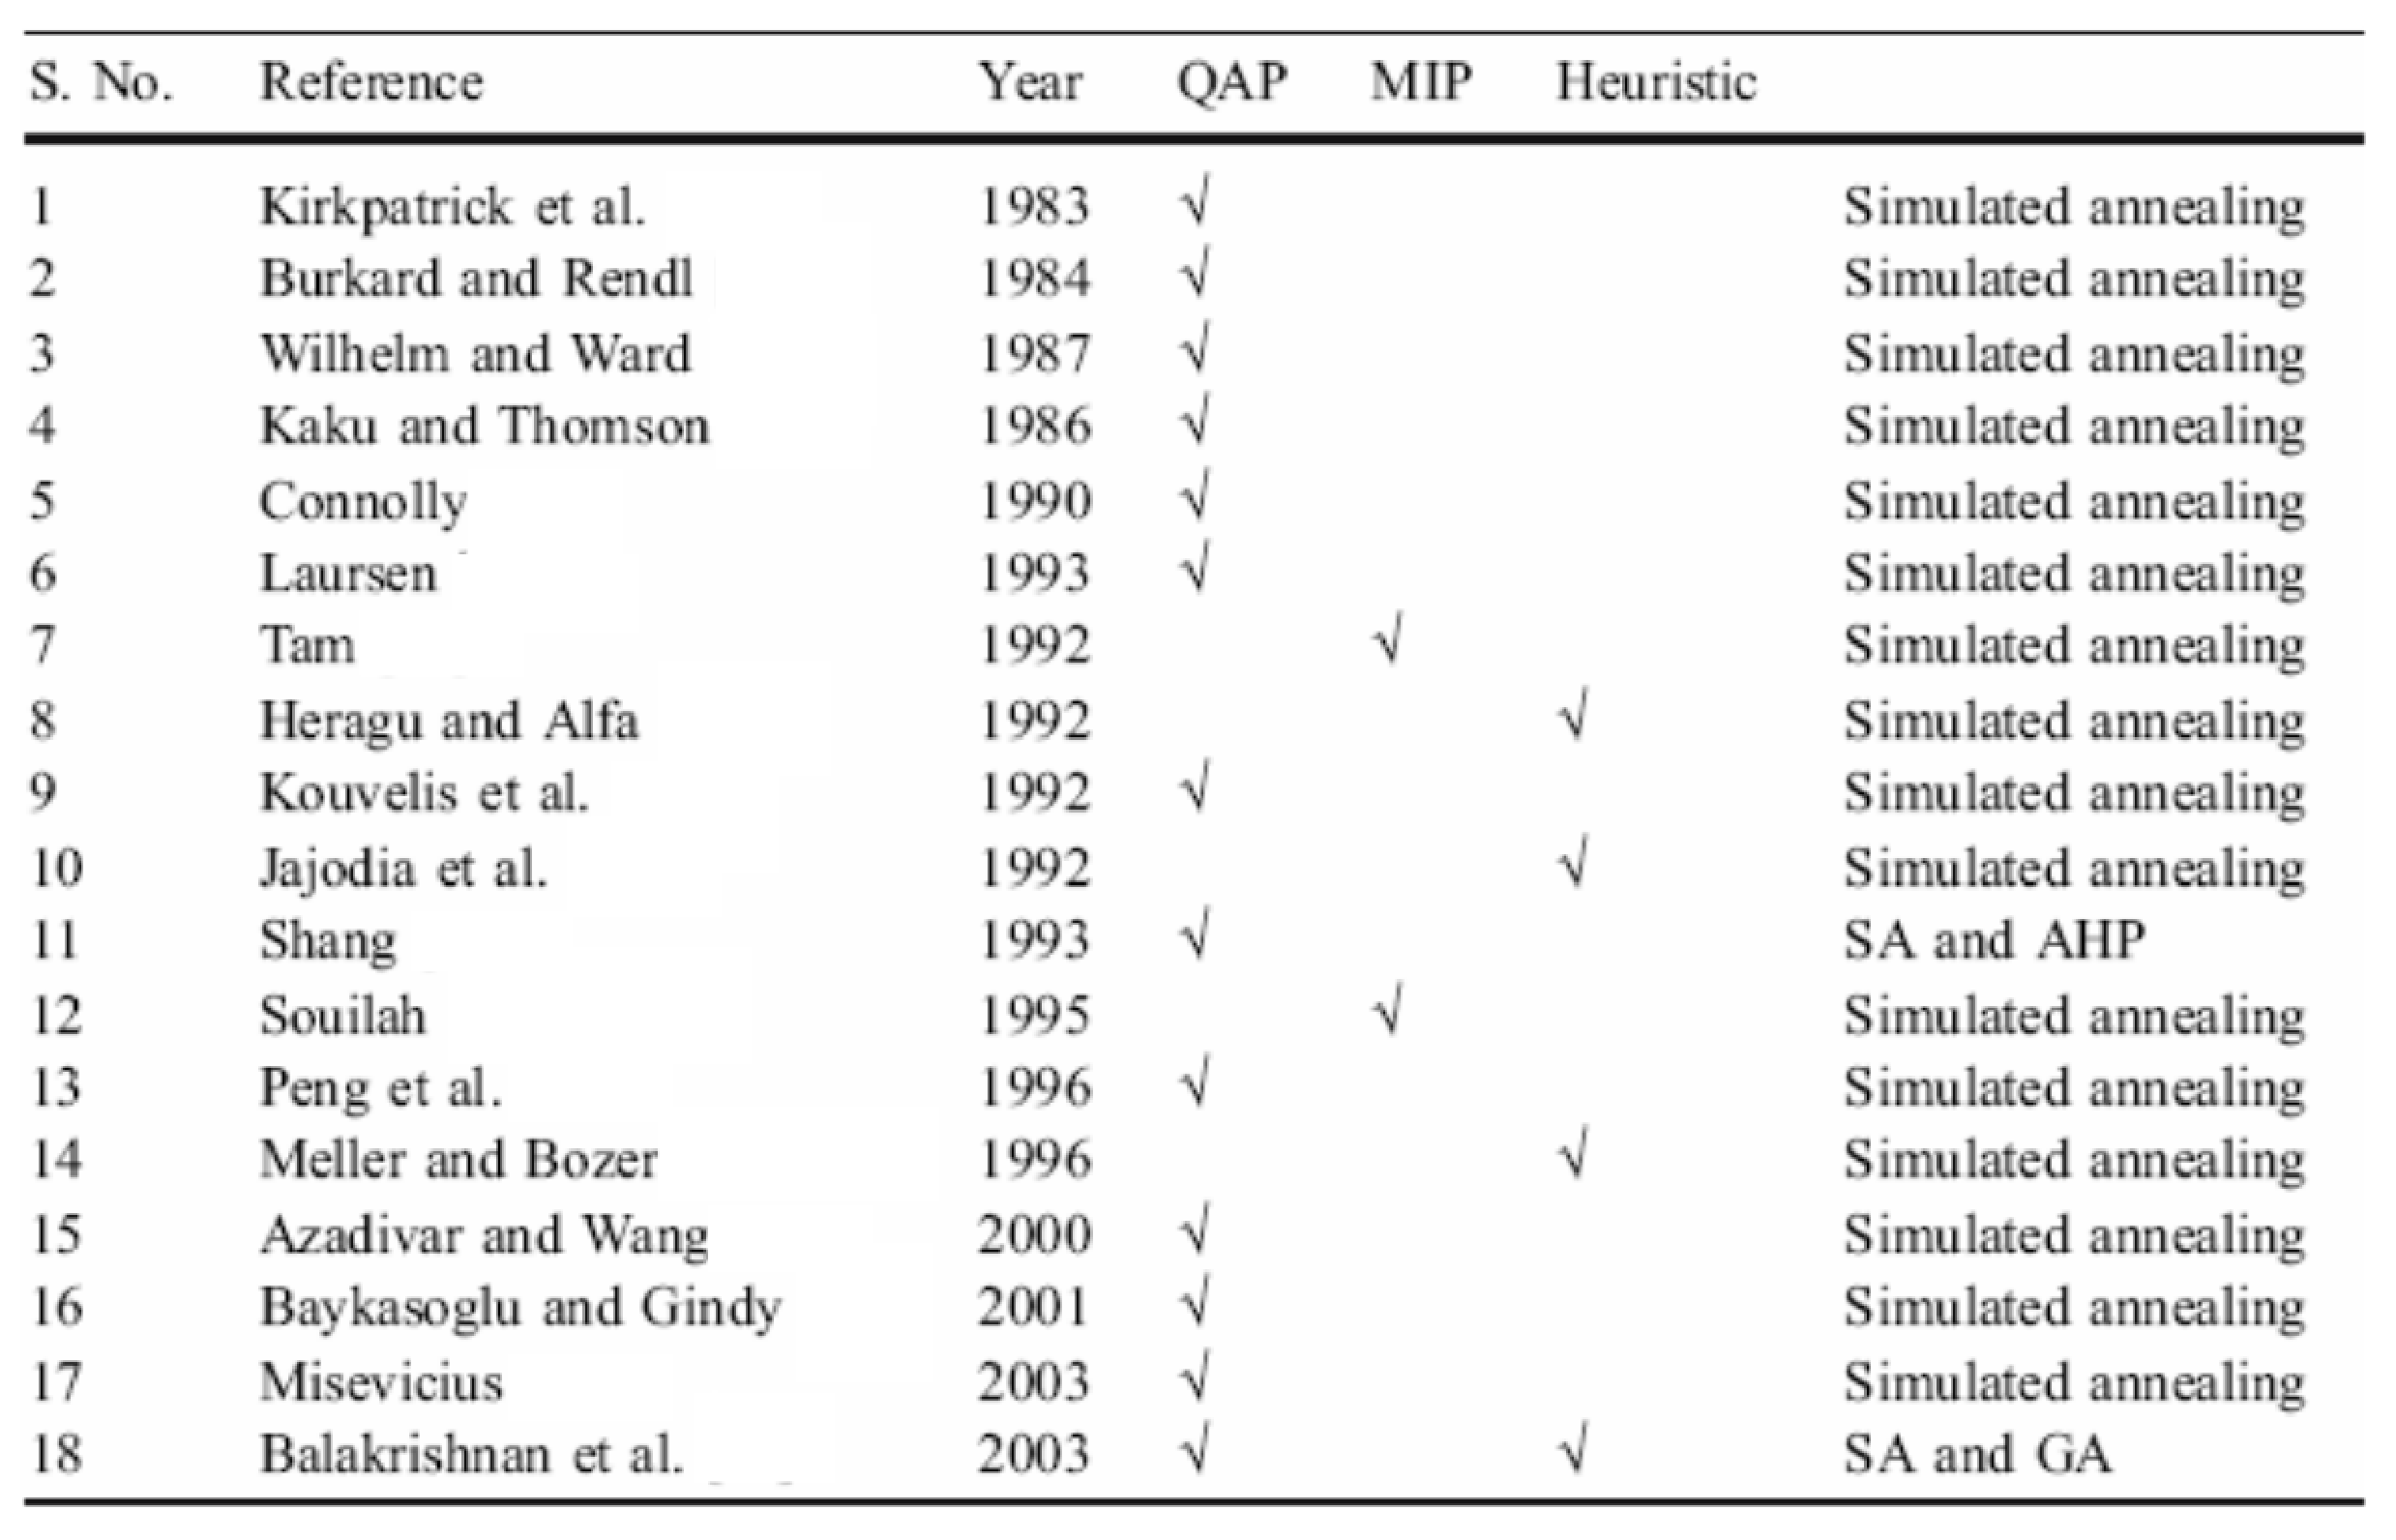
\includegraphics[width=12cm, height=7cm]{images/sim-ann1.eps}
\textit{\caption{\footnotesize raccolta di articoli sugli algoritmi SA per la risoluzione dei FLP}}
\end{figure}\\
Durante l'ultimo decennio anche l'algoritmo genetico ha guadagnato molta attenzione; esso utilizza una codifica binaria di individui come stringhe di lunghezza fissa. GA cerca iterativamente l'ottimo globale, senza esaurire lo spazio delle soluzioni, in un processo parallelo che inizia da un piccolo insieme di soluzioni ammissibili (popolazione) e che genera nuove soluzioni in un qualche modo aleatorio. La performance del GA dipende dal problema perch\'{e} la sistemazione dei parametri e lo schema di rappresentazione dipendono dalla natura del problema. Tavakkoli-Moghaddam e Shayan (1998) hanno analizzato l'adeguatezza degli algoritmi genetici per risolvere il FLP. La tabella di figura 1.20 fornisce recenti articoli sui FLP basati sui GA. Gli algoritmi Tabu-Search (TS) sono altre procedure iterative progettate per risolvere problemi di ottimizzazione. Helm e Hadley (2000) hanno applicato algoritmi TS per la risoluzione del FLP. Il metodo \`{e} ancora molto studiato, ed \`{e} in continua evoluzione e miglioramento. Recentemente, alcuni articoli sono apparsi dove un algoritmo \textit{ant colony} \`{e} stato usato per risolvere FLP di grandi dimensioni. Talbi et al. (2001) hanno usato un algoritmo ant colony per risolvere il QAP.
\begin{figure}[h]
\centering
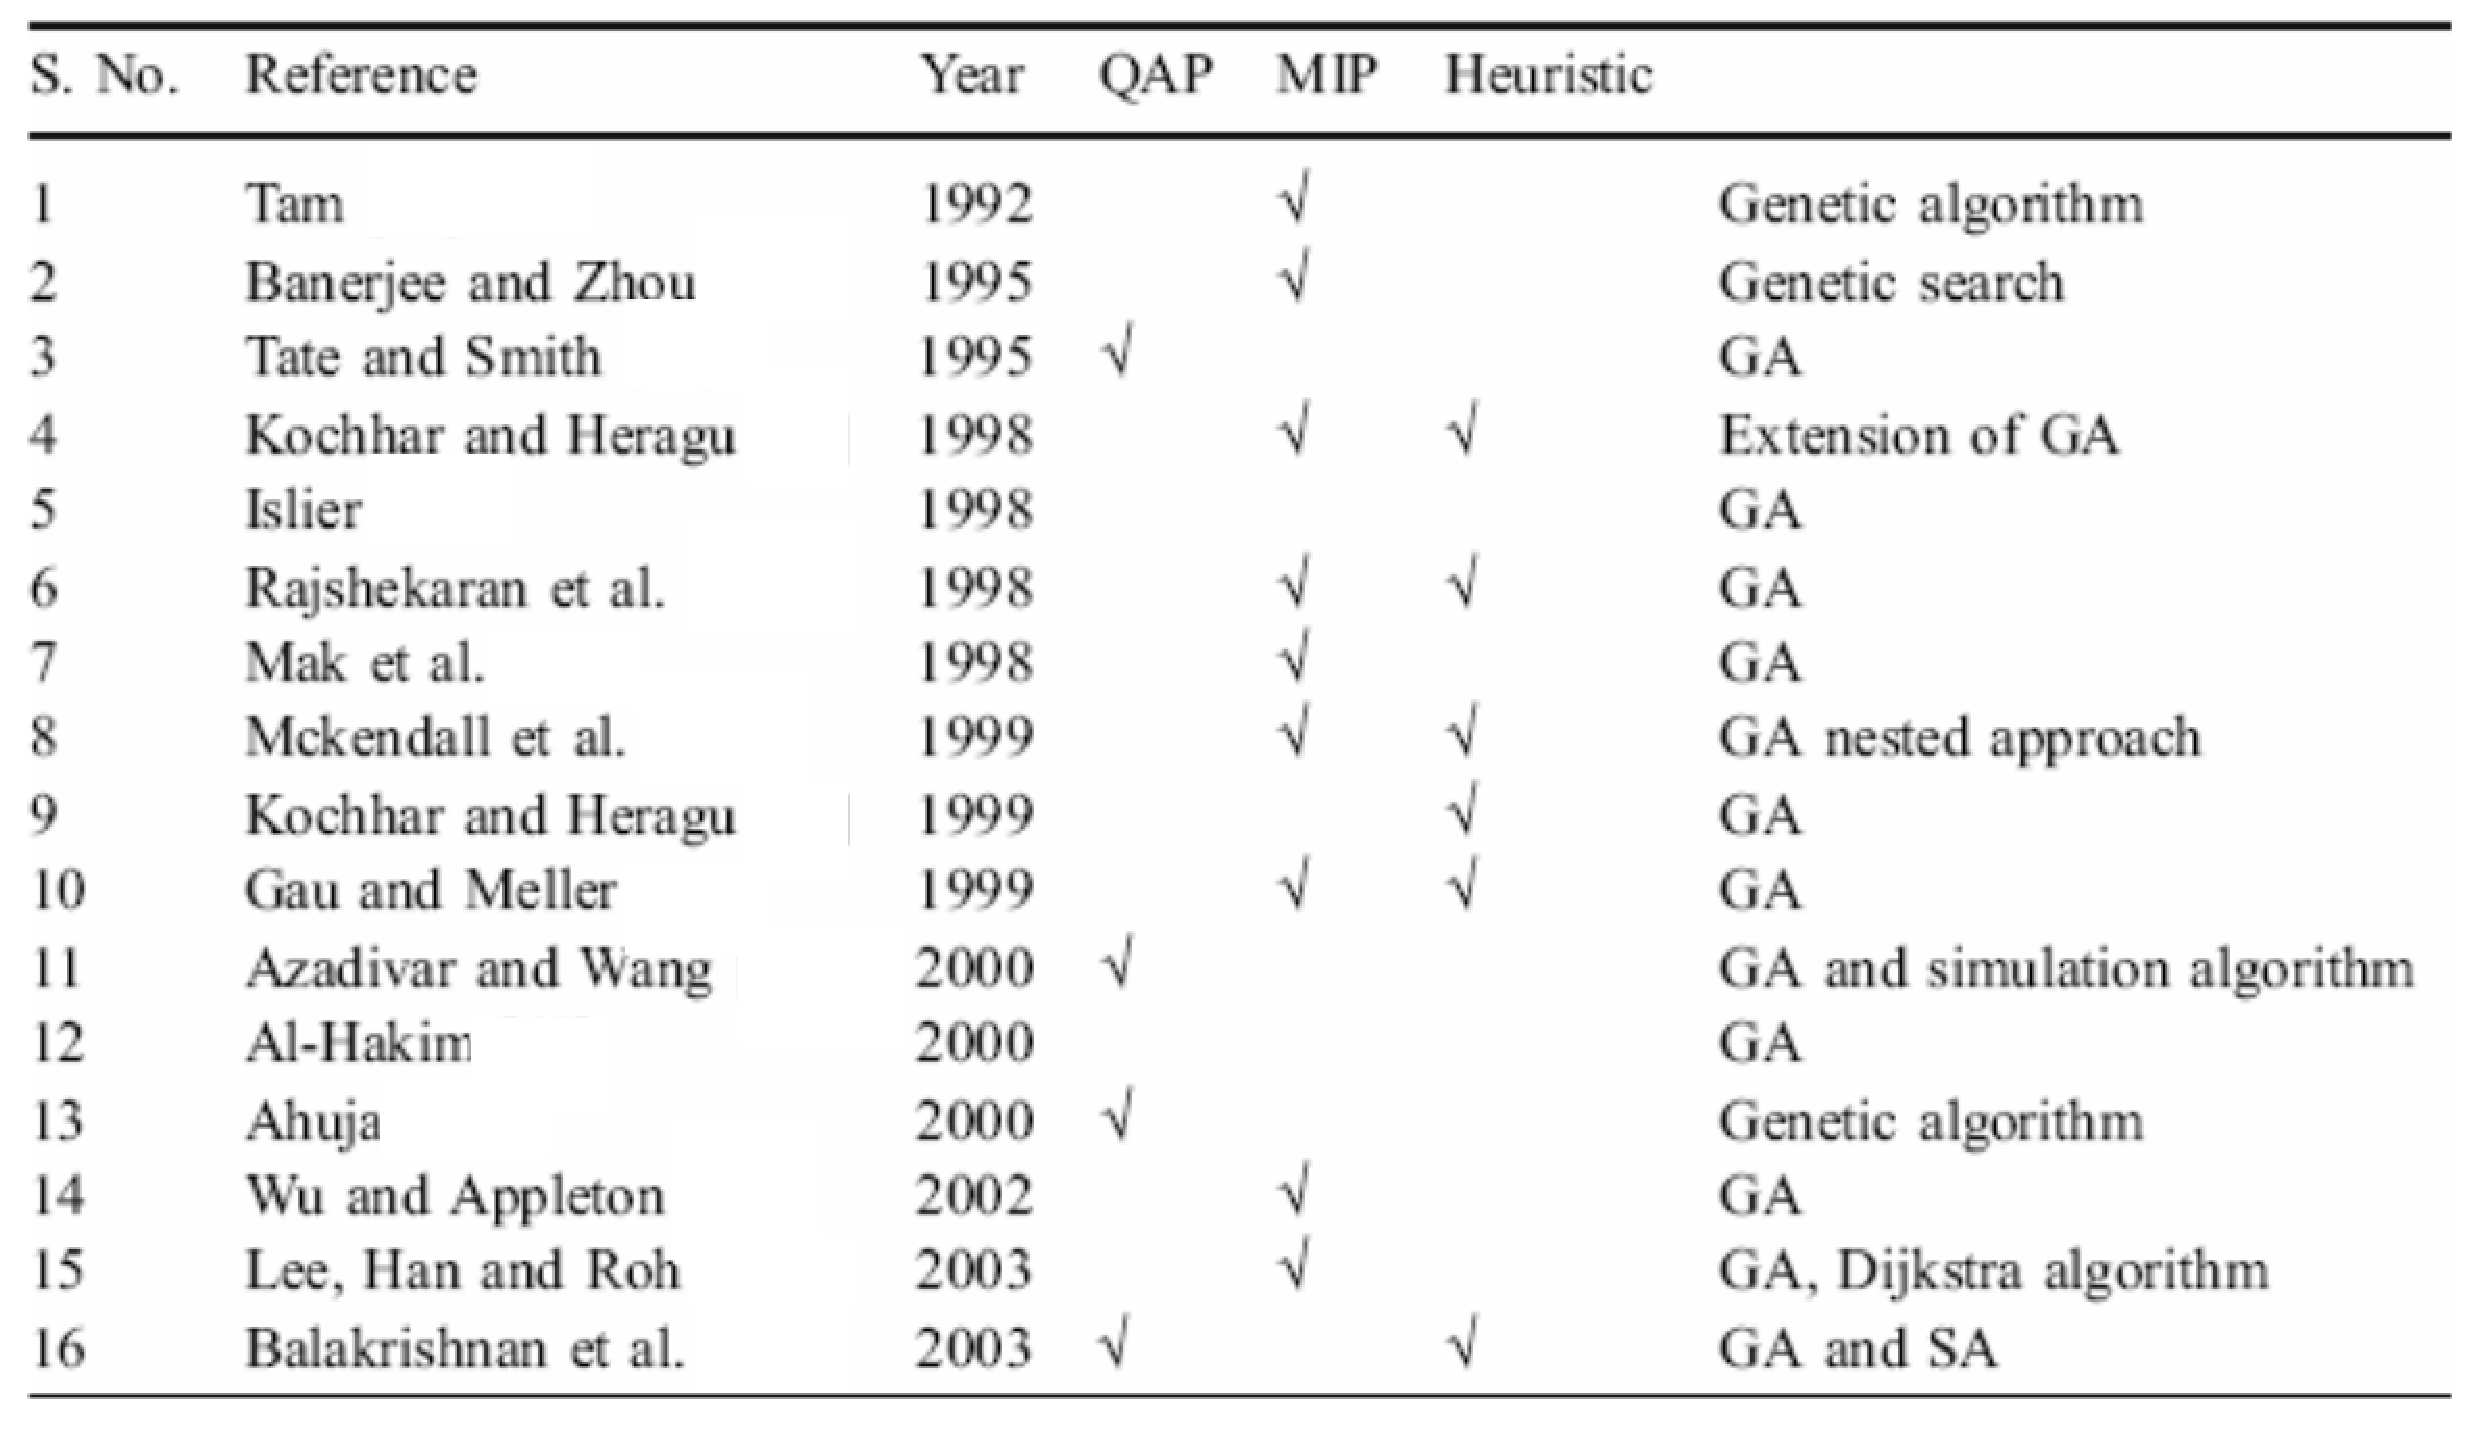
\includegraphics[width=12cm, height=7cm]{images/sim-ann2.eps}
\textit{\caption{\footnotesize raccolta di articoli sugli algoritmi GA per la risoluzione dei FLP}}
\end{figure}

\subsubsection{OBIETTIVI FUTURI E NUOVI SCENARI D'AZIONE}
Dall'analisi delle molteplici alternative riportate in questo paragrafo, si evince che la ricerca sul FLP non \`{e} convergente, ma in qualche modo divergente. Al momenti, l'approccio AI\footnote{Artificial Intelligence} pu\`{o} essere usato per sviluppare euristici che risolvano FLP di grandi dimensioni; inoltre \`{e} necessaria pi\`{u} ricerca nelle funzioni multi-obiettivo per raggiungere criteri di layout pi\`{u} rilevanti. Ogni due anni il \textit{Material Handling Institute of America}, insieme ad altre industri sponsorizzatrici e alle agenzie di governo, organizza un consorzio sulla ricerca riguardo le novit\`{a} sui sistemi di trasporto materiali dove i ricercatori possono presentare le proprie ricerche. \`{E} stato scoperto che c'\`{e} una mancanza di applicazione della \textit{concurrent engineering} nel FLP in accordo con la scelta del sistema di movimentazione materiali che mostra come la progettazione del layout dei macchinari sia indipendente dalla scelta del sistema di movimentazione. \`{E} stato calcolato che lo stesso layout non \`{e} appropriato per tutti i periodi, poich\'{e} la domanda non rimane la stessa. Da qui, la ricerca dovrebbe indirizzarsi verso un layout delle attrezzature dinamico e non statico. Per la risoluzione del FLP sta emergendo soprattutto la ricerca nell'applicazione di meta-euristici come gli algoritmi SA, GA e TS. Tuttavia, il risultato finale dipende anche dalla soluzione iniziale presa (popolazione). Quindi, la ricerca deve anche sviluppare validi euristici che generino buone soluzioni iniziali.
%%%%%%%%%%%%%%%%%%%%%%%%%%%%FINE PRIMO CAPITOLO%%%%%%%%%%%%%%%%%%%%%%%%%%%%%%%
%%%%%%%%%%%%%%%%%%%%%%%%%%%%%%%%%%%%%%%%%%%%%%%%%%%%%%%%%%%%%%%%%%%%%%%%%
\newpage
\chapter{Ottimizzazione dei layout fieristici}                   %crea il capitolo
%%%%%%%%%%%%%%%%%%%%%%%%%%%%%%%%%%%%%%%%%imposta l'intestazione di pagina
Prendendo spunto dalle numerose fonti disponibili sul web o dai documenti a riguardo, si pu\`{o} riassumere brevemente lo scopo primario di una buona progettazione del layout, sia dal punto di vista aziendale che organizzativo (per eventi, fiere, manifestazioni, ecc.).
\begin{quotation}
\emph{L'organizzazione vera e propria dello spazio di vendita (layout) prevede il disegno dei percorsi e della circolazione, in cui la sequenza delle aggregazioni merceologiche deve risultare naturale e di facile lettura per la propria clientela-obiettivo. Generalmente si crea un percorso principale, che stimoli il cliente a seguirlo, e spazi di viabilit\`{a} secondaria, all'interno delle diverse are del punto vendita. Nel fare ci\`{o} ci si deve assicurare che i percorsi siano sufficientemente ampi da garantire il passaggio agevole della clientela e dei commessi, eliminandone i punti morti. La presenza di un'illuminazione studiata e di una segnaletica efficace ma non invasiva deve, inoltre, guidare l'attenzione dei clienti verso i punti di maggiore attrattiva del locale.}
\end{quotation}
In particolare, nel corso del presente capitolo, verr\`{a} focalizzata l'attenzione sull'analisi di casi di studio noti, quali le fiere di Fortaleza in Brasile e di Romont in Svizzera. Tali informazioni e dati sono infatti molto utili come modello per lo sviluppo e l'applicazione degli algoritmi visti nel primo capitolo all'ambito fieristico.
\section{Specifiche e contesti per il progetto}
L'obiettivo principale del progetto di un layout fieristico consiste nel posizionare il massimo numero di stand nell'area adibita all'esposizione, soddisfacendo un certo numero di requisiti operazionali (\textit{constraints}).
Data una superficie $S$ adibita all'esposizione, di forma irregolare e non convessa, e un numero $n$ di stand uguali e rettangolari, si vuole massimizzare il numero di stand contenuti in $S$ cercando allo stesso tempo di ottenere un layout che possa rispondere alle esigenze di un contesto fieristico. Un layout si dice "`"`fattibile"'"' se soddisfa un certo numero di \textit{constraints} di base (tipici di un contesto fieristico) pi\`{u} altri requisiti specifici forniti dall'organizzazione nel caso specifico.
Si possono riassumere le condizioni di "`"`fattibilit\`{a}"'"' del layout nei seguenti punti comuni ad ogni organizzazione fieristica:
\begin{itemize}
\item gli stands non possono sovrapporsi
\item gli stands devono essere completamente contenuti nella superficie $S$
\item i visitatori (ma anche gli organizzatori) devono poter facilmente accedere agli stands
\end{itemize}
Oltre a tali requisiti generici, ogni organizzazione ha anche altre necessit\`{a} proprie, per le quali \`{e} opportuno considerare altri constraints da inserire nel progetto. Un problema simile gi\`{a} ampiamente studiato \`{e} quello concernente l'ottimizzazione dei layout industriali; si usa il termine "`"`simile"'"' e non il termine "`"`uguale"'"' perch\'{e} nell'ambito delle fiere non bisogna tenere conto del flusso: tra uno stand e uno altro non vi \`{e} nessun flusso di materiale come invece accade tra un macchinario ed un altro in un'impresa manifatturiera. Il problema del layout fieristici sembra piu vicino a quello del \textit{packing}, in particolare il \textit{two dimensional packing problem}\footnote{appunto perch\'{e} si ha a che fare con un problema di packing, allora si inserisce tale prolema nell'insieme degli NP-hard (considerando il caso pi\`{u} generale in cui ogni stand pu\`{o} essere ruotato in ogni direzione possibile)}. Tuttavia si tratta di un task di grande interesse nel campo dell'ottimizzazione combinatoria, essendo un campo di applicazione piuttosto nuovo; come ulteriore complicazione, rispetto ai casi generali di packing NP-hard, per un contesto fieristico nasce il problema legato alla irregolarit\`{a} della superficie espositiva. Un esempio di superficie irregolare \`{e} quello di figura 2.1:
\begin{figure}[h]
\centering
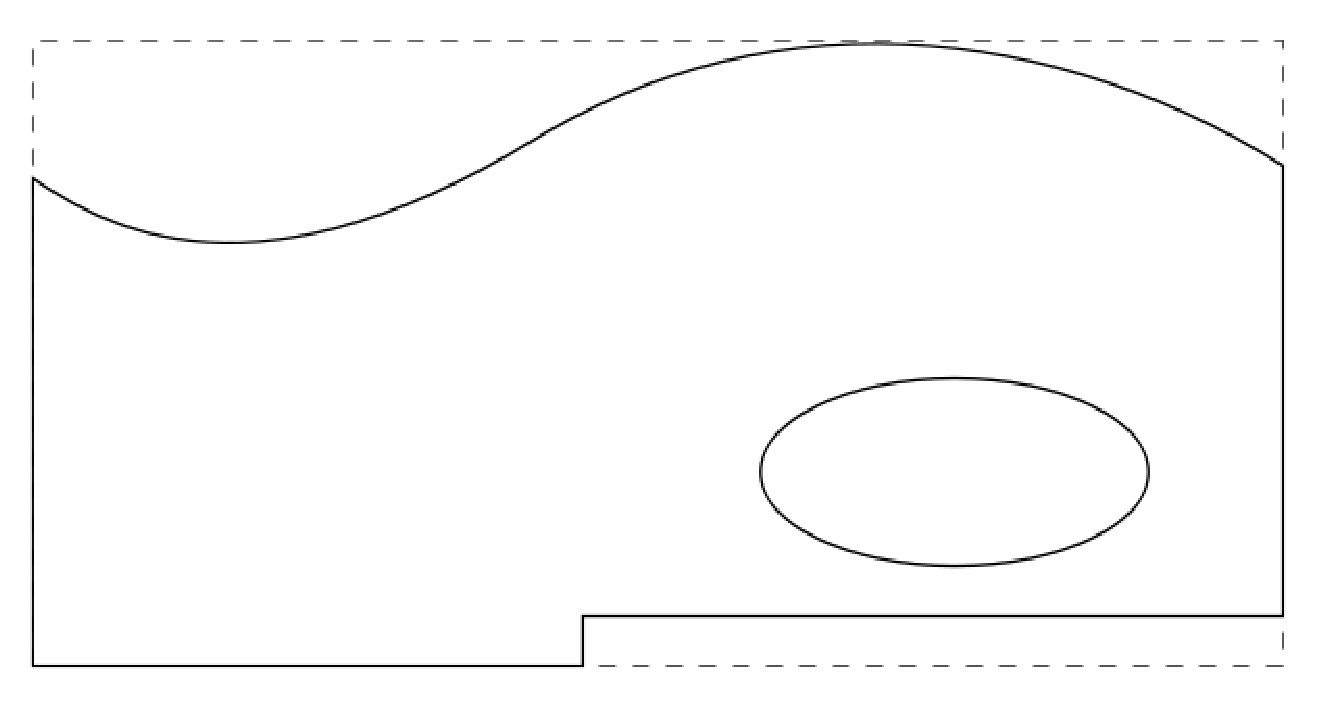
\includegraphics[width=9cm, height=5cm]{images/area1.eps}
\textit{\caption{\footnotesize tipico esempio di superficie irregolare su cui progettare il layout}}
\end{figure}  
\\Accanto a questo importante e determinante \textit{constraint} le specifiche, piuttosto comuni nella maggioranza dei casi, impongono anche di considerare gli stands orientati tutti nello stesso modo e allineati tutti nella stessa direzione lungo striscie verticali; ovviamente sar\`{a} opportuno riservare uno spazio minimo tra tali striscie per permettere un accesso facile alla clientela.
Nel progettare un layout siffatto \`{e} bene tenere in considerazione tre obiettivi fondamentali, associati ad altrettante funzioni obiettivo:
\begin{itemize}
\item l'utilizzo ottimo dello spazio a disposizione
\item lo scopo di attirare la maggiore clientela possibile
\item la convenienza dal lato cliente
\end{itemize}
Ovviamente, come gi\`{a} detto in precedenza, si tratta di un tipico problema di 2BPP e di FLP, analizzati nel capitolo precedente. In particolare \`{e} opportuno considerare un impaccamento di questo tipo \`{e} chiamato in letteratura \textit{two-dimensional two-staged packing}; si supponga che si voglia tagliare l'area per l'esposizione per produrre una serie di aree pi\`{u} piccole rappresentanti gli
stand, ci\`{o} pu\`{o} essere fatto grazie a una prima fase di tagli a ghigliottina paralleli al lato rappresentante l'altezza e a una seconda fase in cui si eseguono tagli, sempre a ghigliottina, paralleli al lato rappresentante la larghezza. Nella seconda fase \`{e} necessario effettuare un taglio per ogni striscia ottenuta nella prima fase.\\
\\Riassumendo i principali puti salienti del problema, possiamo descrivere come operare seguendo una serie di accorgimenti e metodi risolutivi che indichiamo come \textit{Fair Layout Optimization Problem} (FLOP). Si considerino le seguenti assunzioni:
\begin{description}
\item[assunzione 1]: l'area su cui progettare \`{e} una superficie\footnote{da qui deriva il fatto che si progetta su due dimensioni} irregolare, contenuta in un rettangolo di altezza $H$ e larghezza $W$ che la incapsula in modo preciso (vedere le linee tratteggiate di figura 2.1); 
\item[assunzione 2]: gli stands sono rettangoli tutti identici e hanno altezza $h$ e larghezza $w$ 
\item[assunzione 3]: non sono ammesse rotazioni degli stands (tutti devono essere orientati allo stesso modo)
\item[assunzione 4]: l'allocazione deve essere fatta ortogonalmente su striscie (\textit{strips}) verticali parallele ai lati verticali del rettangolo, garantendo l'accesso da uno dei lati liberi per ciascuno stand
\end{description}  
A questo proposito si proceder\`{a} secondo una duplice variante del FLOP cercando di impaccare il massimo numero di stand nella superficie a disposizione in modo da non violare tutte le considerazioni fatte in precedenza e soddisfacendo le assunzioni appena fatte.
\begin{center}
\begin{itemize}
\item FLOP 1: viene richiesto che ogni stand (ogni strip) possa essere acceduto da ambo i lati (striscie singole)
\item FLOP 2: \`{e} possibile disporre gli stand in striscie accoppiate senza spazi tra di esse, in modo che l'accesso agli stand avvenga dal solo lato libero
\end{itemize}
\end{center}
In figura 2.2 sono illustrate le due varianti FLOP1 e FLOP2 rispettivamente.
\begin{figure}[h]
\centering
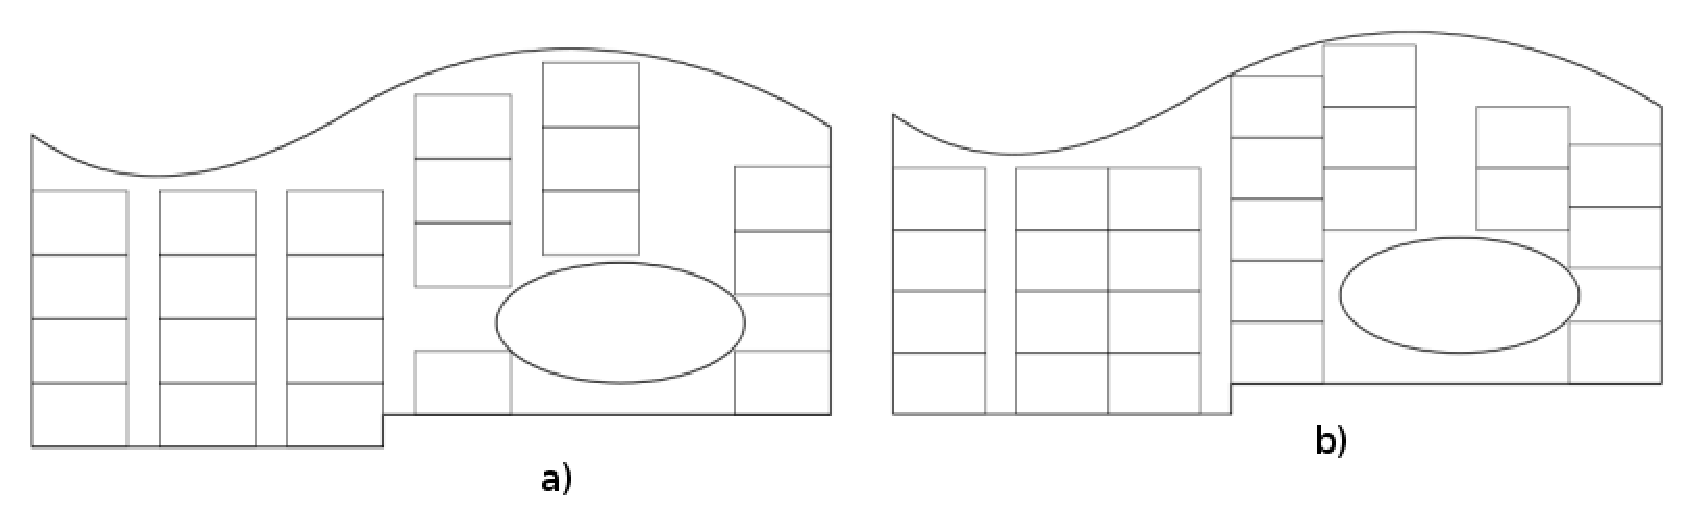
\includegraphics[width=12.5cm, height=4.5cm]{images/area2.eps}
\textit{\caption{\footnotesize varianti del progetto: a) = FLOP1 (a sinistra) e b) = FLOP2 (a destra)}}
\end{figure}  
Senza perdere di generalit\`{a}, assumeremo che la superficie sia accessibile da tutte le parti. 
Se si considera l'area espositiva come una matrice binaria $M$ con $H$ righe e $W$ colonne, corrispondente al rettangolo sopracitato, numerando righe e colonne dall'angolo in basso a sinistra della matrice (si considerino le due dimensioni della superficie come su di un piano cartesiano), si definisce la matrice come:
$$ 
M_{i,j} =  
\left\{
\begin{array}{rl}
1 & \mbox{se lo spazio } \delta \times \delta \mbox{ alle coordinate (i,j) viene allocato per lo stand}\\
0 & \mbox{altrimenti}
\end{array}
\right.
$$
dove, per semplicit\`{a} si considerano tutte le variabili (altezze, larghezze, distanze, ecc.) come valori interi, espressi secondo una unit\`{a} minima di lunghezza che indichiamo con $\delta$, mentre $i = 1,...,H$ e $j = 1,...,W$.
\begin{figure}[h]
\centering
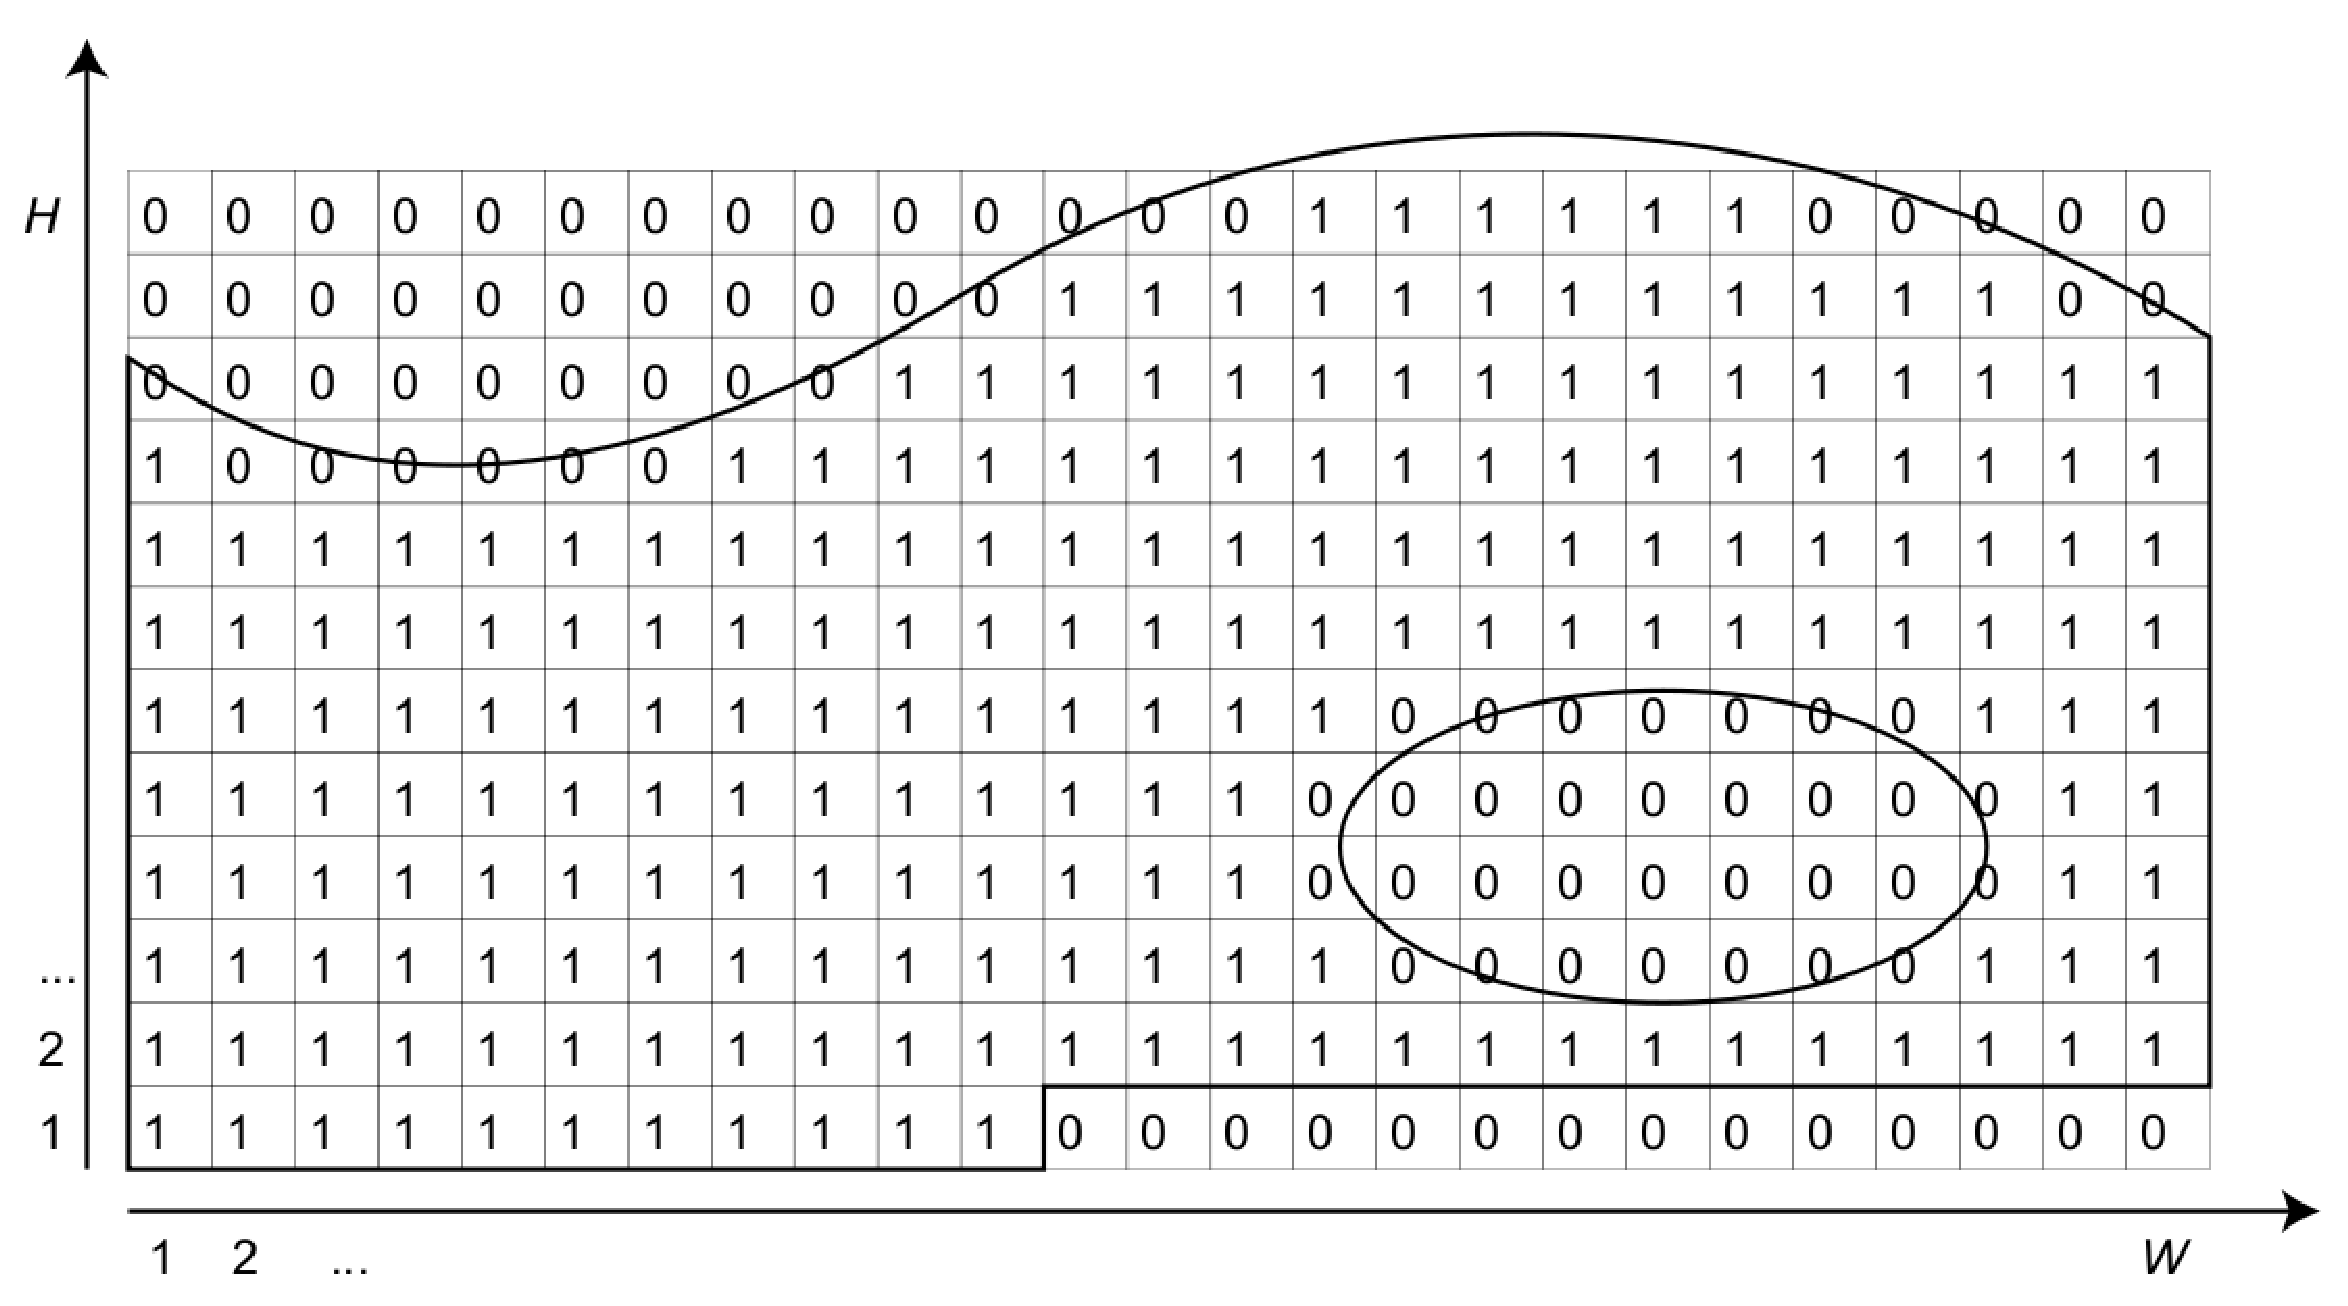
\includegraphics[width=9.5cm, height=5.5cm]{images/area3.eps}
\textit{\caption{\footnotesize matrice M associata all'area di esposizione fieristica di figura 2.1}}
\end{figure} 
Pertanto si seleziona una colonna $j$ per il layout nel caso in cui una striscia di stands (\textit{strip}) sia posizionata sulla colonna stessa col lato sinistro: ad esempio in figura 2.1 e 2.2 la prima colonna viene selezionata come prima strip (dove $w=3$, $h=2$). 
Supponiamo che ciascuna colonna $j$ e ciascun intervallo massimo di righe $[i_{a}, i_{b}]$ di $M$ formino una sottomatrice avente tutti $1$ come suoi elementi: tali elementi della sottomatrie ottenuta saranno rettangoli di larghezza $w$ e altezza $(i_{b}-i_{a}+1)$ col proprio vertice in basso a sinistra alla coordinata $(i_{a},j)$.
Di consegienza, il massimo numero di stands che possono essere piazzati all'interno di tale sottomatrice \`{e} $\lfloor \dfrac{i_{b}- i_{a}}{h} \rfloor$. In figura 2.3 ad esempio, si contano per $j=W-3$, due intervalli massimi di righe di larghezza 3: uno alto 2 e l'altro alto 5; la striscia corrispondente pu\`{o} quindi disporre di tre stands in totale.\\
Per ogni colonna $j \leq W - w + 1$, il massimo numero di stands $v_{j}$ che possono essere posizionati col loro lato sinistro nella colonna $j$ \`{e} ottenuto in maniera iterativa, determinando le successive colonne che soddisfino le condizioni specificate.
Una schietta implementazione di questo metodo richiederebbe, per ogni colonna, un numero di iterazioni pari a $O(H)$ di complessit\`{a} temporale pari a $O(w)$; quindi in totale un tempo $O(W H w)$.\\
\\Una procedura pi\`{u} veloce che richiede un tempo $O(W H)$ pari a quello impiegato per "`"`caricare"'"' la matrice M sar\`{a} illustrata di seguito; tale procedura calcola le stesse informazioni $v_{i} (j=1,...,W-w+1)$.
\begin{figure}[h]
\flushleft
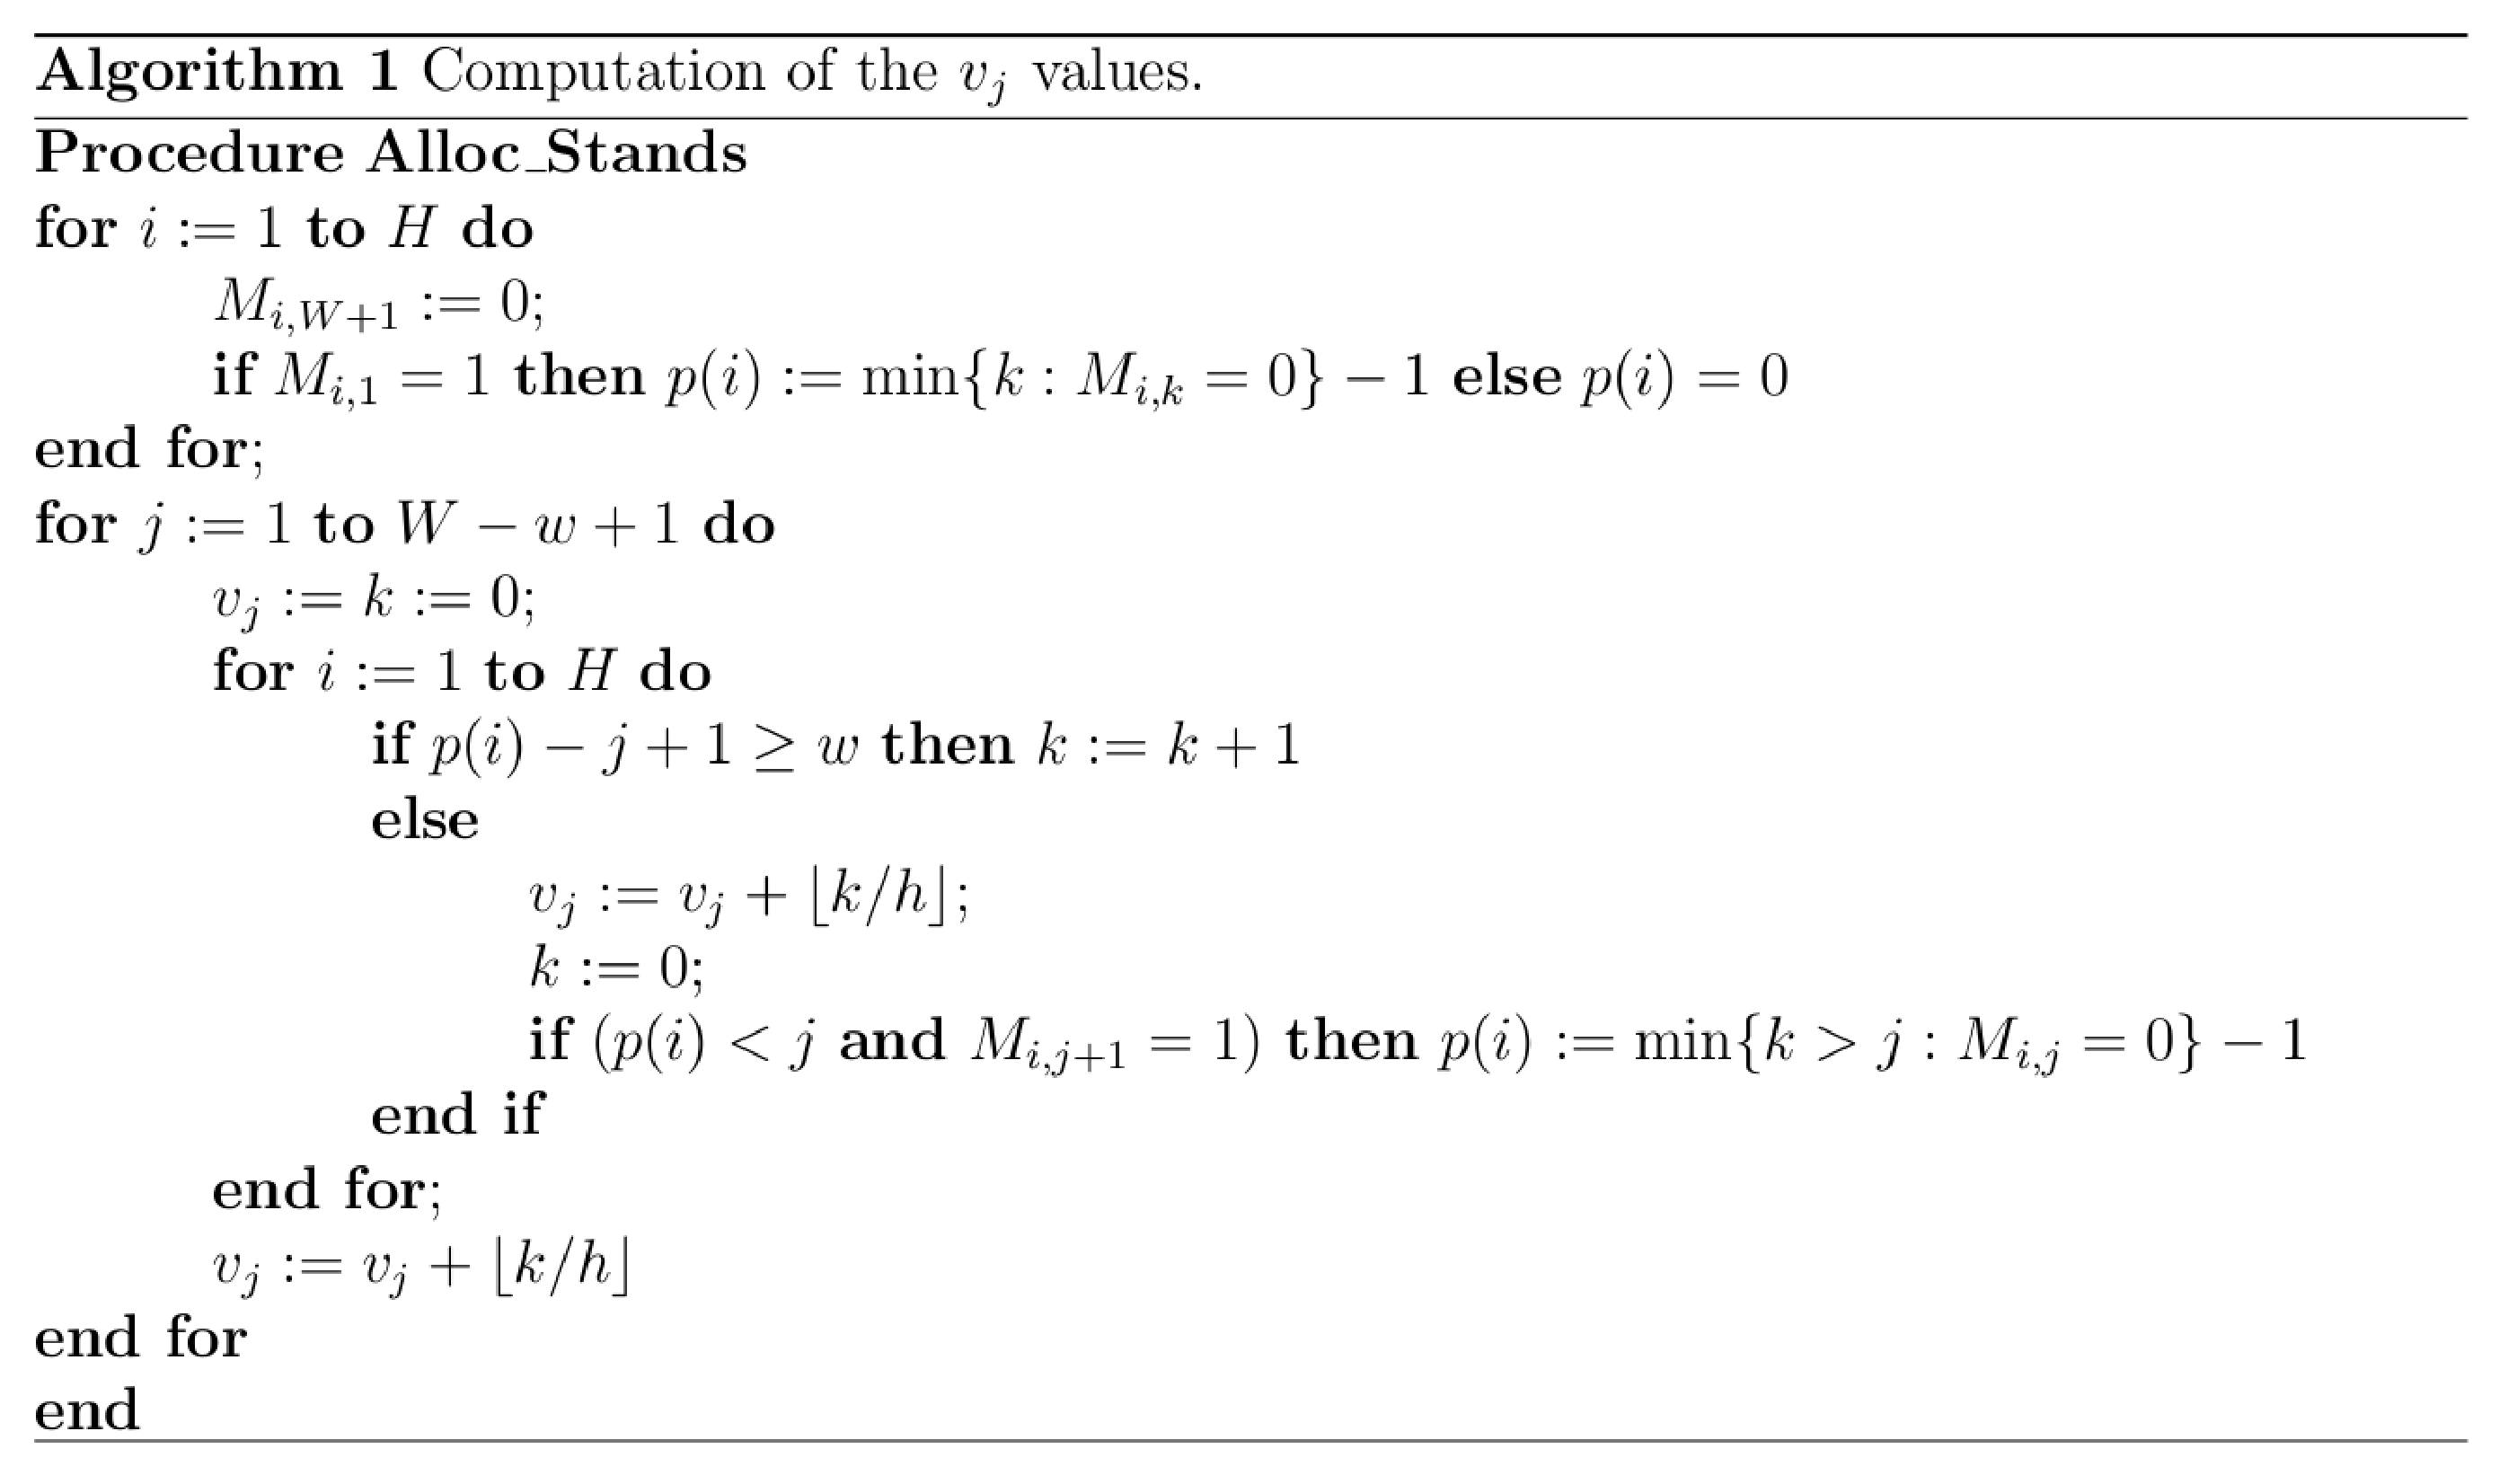
\includegraphics[width=14.8cm, height=9cm]{images/algorithm.eps}
\end{figure}
\\Si analizzi l'algoritmo: definiamo, per ogni riga $i$ che sia $M_{i,j}=1$, un puntatore $p(i)$ all'ultima colonna $\hat{j}$ in modo che sia $M_{i,j} = M_{i,j+1} = ... = M_{i, \hat{j}} = 1$. Se invece $M_{i,j}=0$ per la colonna corrente $j$, allora $p(i)$ avr\`{a} un qualsivoglia valore minore di $j$; in questo modo tutti gli intervalli massimi di riga possono essere determinati esaminando ogni elemento di $M$ un numero fisso e costante di volte. La variabile contatore $k$ memorizza, per la colonna corrente $j$ e per l'attuale intervallo di riga, il numero di righe che soddisfano le specifiche e che quindi definiamo "`"`idonee"'"'.\\
Il nostro problema di ottimizzazione combinatoria si focalizza perci\`{o} nella determinazione delle colonne $j$ che possono essere inserite nell'impaccamento delle \textit{strips} di stands.  

\subsection{Modelli matematici}
Nel presente paragrafo si analizzeranno i due modelli matematici corrispondenti alle due varianti di \textit{fair layout optimization problem} introdotte in precedenza. 
La prima parte, dedicata al FLOP1, non prevede alcuna richiesta riguardante la distanza tra due \textit{strips} diverse di stands; inoltre si fa riferimento alle assunzioni 1-4 viste precedentemente.
Consideriamo una variabile binaria 
\begin{equation}\label{eq1}
x_{j}=
\left\{
\begin{array}{ll}
1 \mbox{ se una strip \underline{singola} di stands ha il proprio lato sinistro sulla colonna j} \\
0 \mbox{ altrimenti}
\end{array}
\right.
\end{equation}
$$\forall j = 1,...,W - w + 1.$$
Il primo problema \textbf{FLOP1} pu\`{o} quindi essere modellato come segue:
\begin{equation}\label{eq2}
\mbox{(FLOP1) } max \sum_{j=1}^{W-w+1}v_{j}x_{j} 
\end{equation}
\begin{equation}\label{eq3}
\mbox{subject to } \sum_{j=k-a-w+1}^{k} x_{j} \leq 1 \mbox{ , } (k = w+a,...,W-w+1) 
\end{equation}
\begin{equation}\label{eq4}
x_{j} \in \left\lbrace 0,1 \right\rbrace \mbox{ , } (j=1,...,W-w+1) 
\end{equation}
dove $a$ rappresenta la larghezza minima del passaggio pedonale tra strips\footnote{che in inglese si indica con \textit{aisle=navata} come si pu\`{o} vedere in figura 2.5}. Dalla espressione (\ref{eq3}) si nota che i vincoli impongono che gli stands non si sovrappongano tra loro e che ci sia spazio sufficiente per le \textit{aisles}: se una colonna $k$ viene selezionata allora le colonne ($k - a - w +1,..., k-1$) non possono essere selezionate a loro volta, come \`{e} possibile constatare dalla figura 2.4. \`{E} inoltre possibile notare che le constraints (\ref{eq3}) per ($k = 1,...,w+a-1$) non sono imposte, bens\`{i} derivano dal primo vincolo ($k=w+a$).
\begin{figure}[h]
\centering
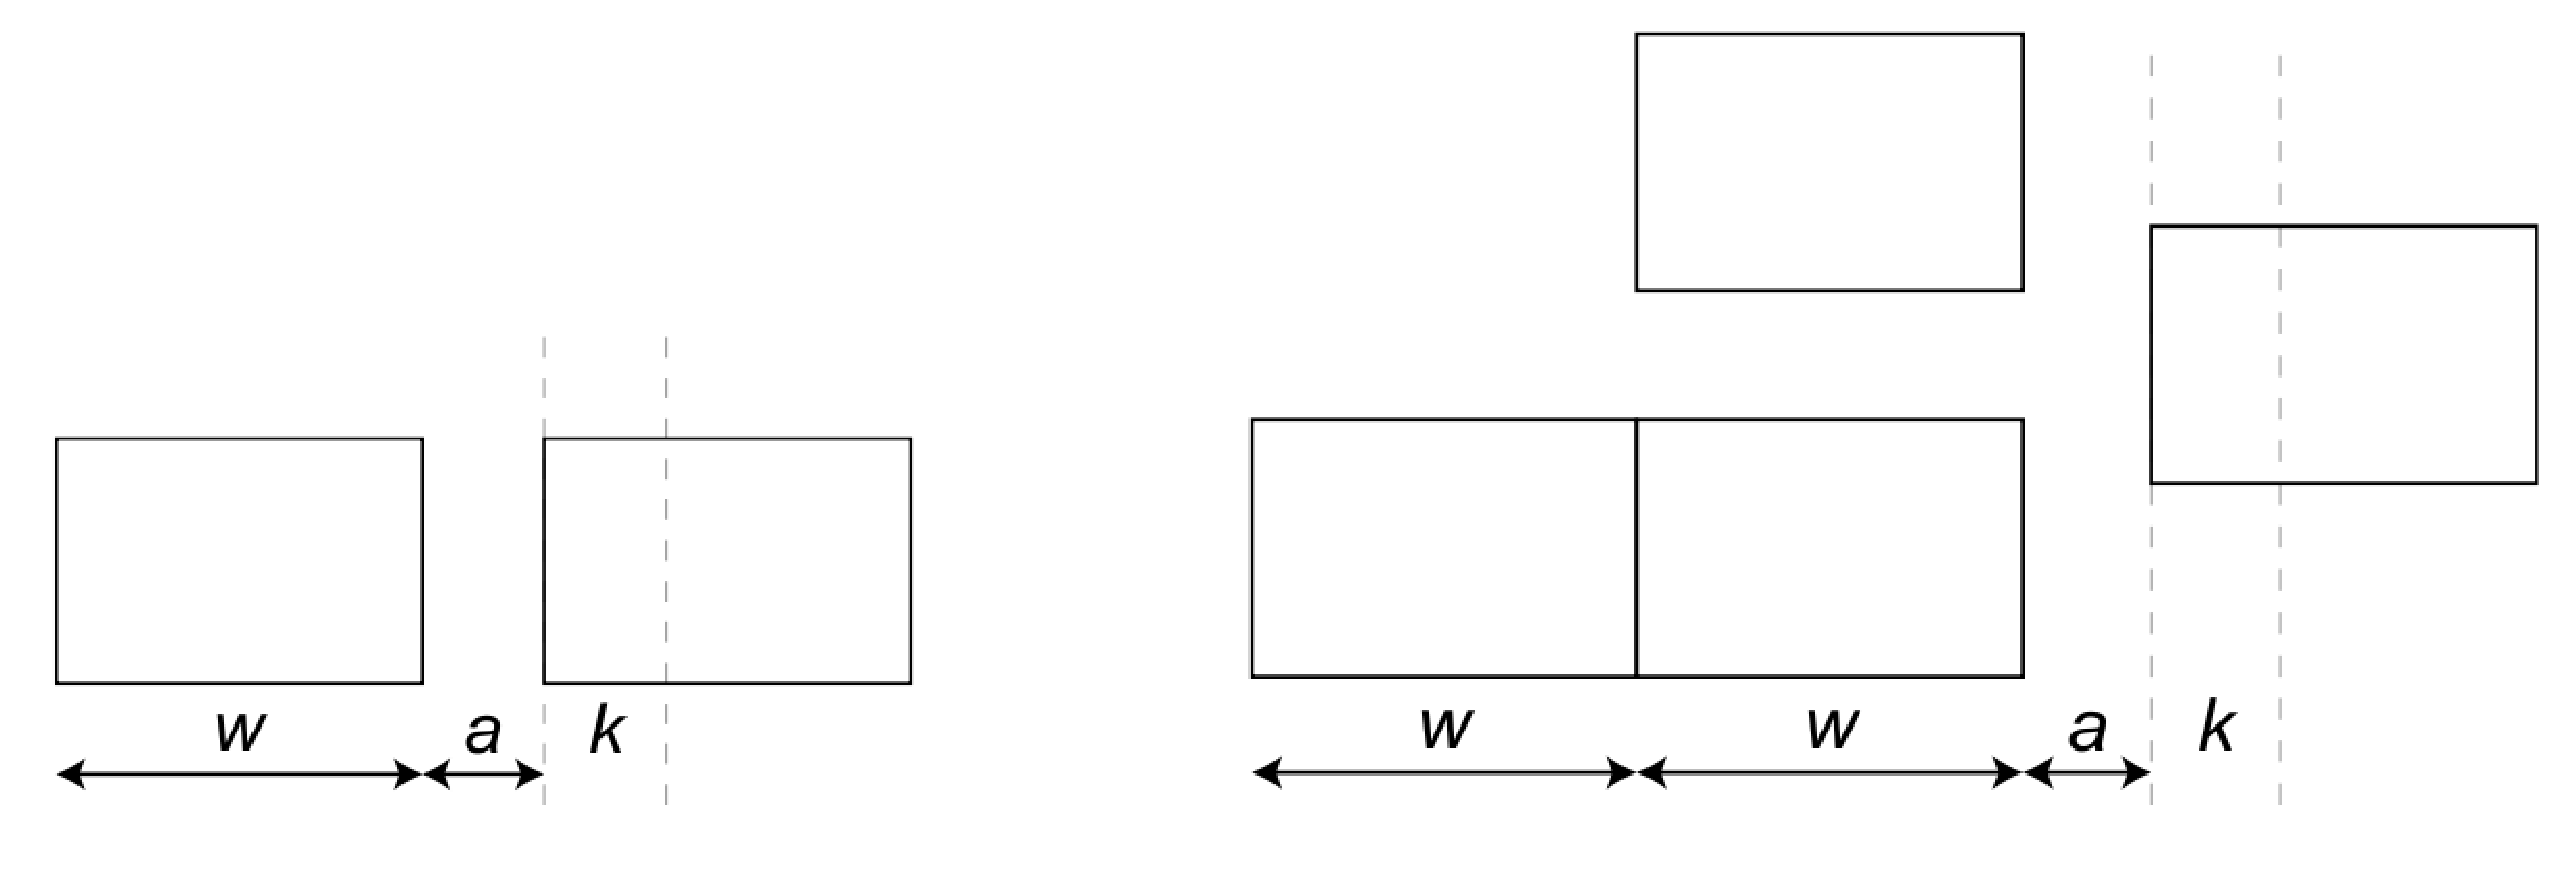
\includegraphics[width=12cm, height=5.5cm]{images/constraints.eps}
\textit{\caption{\footnotesize constraints per il FLOP1 (sinistra) e per il FLOP2 (destra)}}
\end{figure}
\\Il secondo problema FLOP2 pu\`{o} essere modellato analogamente all'algoritmo precedente, introducendo un secondo tipo di variabile binaria per ogni colonna $j$:
\begin{equation}\label{eq4}
\xi_{j}=
\left\{
\begin{array}{ll}
1 \mbox{ se una strip \underline{doppia} di stands ha il proprio lato sinistro sulla colonna j} \\
0 \mbox{ altrimenti}
\end{array}
\right.
\end{equation}
$$\forall j = 1,...,W - 2w + 1.$$
Osserviamo che il massimo numero di stands idonei ad essere compresi nella \textit{double-strip} \`{e} $v_{j}+v_{j+w}$. 
\\Ne deriva quindi il modello \textbf{FLOP2} seguente: 
\begin{equation}\label{eq5}
\mbox{(FLOP2) } max \sum_{j=1}^{W-2w+1}(v_{j}+v_{j+w}) \xi_{j} 
\end{equation}
\begin{equation}\label{eq6}
\mbox{subject to } \sum_{j=k-a-w+1}^{k} x_{j} + \sum_{j=max(1, k-a-2w+1)}^{min(W-2w+1, k)} \xi_{j} \leq 1 \mbox{ , } (k = w+a,...,W-w+1) 
\end{equation}
\begin{equation}\label{eq7}
x_{j} \in \left\lbrace 0,1 \right\rbrace \mbox{ , } (j=1,...,W-w+1) 
\end{equation}
\begin{equation}\label{eq8}
\xi_{j} \in \left\lbrace 0,1 \right\rbrace \mbox{ , } (j=1,...,W-2w+1) 
\end{equation}
Analogamente al caso del FLOP1, qui i vincoli (\ref{eq6}) impongono che le striscie (singole e doppie) di stands non si sovrappongano e che ci sia, come al solito, spazio sufficiente per consentire il flusso dei clienti: se una colonna $k$ viene selezionata (sia se singola sia se doppia), allora le colonne $k-a-w+1,...,k-1$ non possono esserlo altrettanto (nel caso di una \textit{single-strip}), mentre le colonne $k-a-2w+1,...,k-1$ non possono esserlo altrettanto (nel caso di una \textit{double-strip}).
Si pu\`{o} notare che gli indici $max$ e $min$ nella seconda sommatoria della equazione (\ref{eq6}) escludono l'indice $j$ poich\`{e} \`{e} fuori dal range.\\ Nella parte destra di figura 2.4 si pu\`{o} osservare l'insieme di constraint utilizzate per il FLOP2, mentre nelle figure 2.5 e 2.6 \`{e} possibile vedere un esempio di layout che tiene conto di entrambe le varianti FLOP1 e FLOP2.
\begin{figure}[h]
\centering
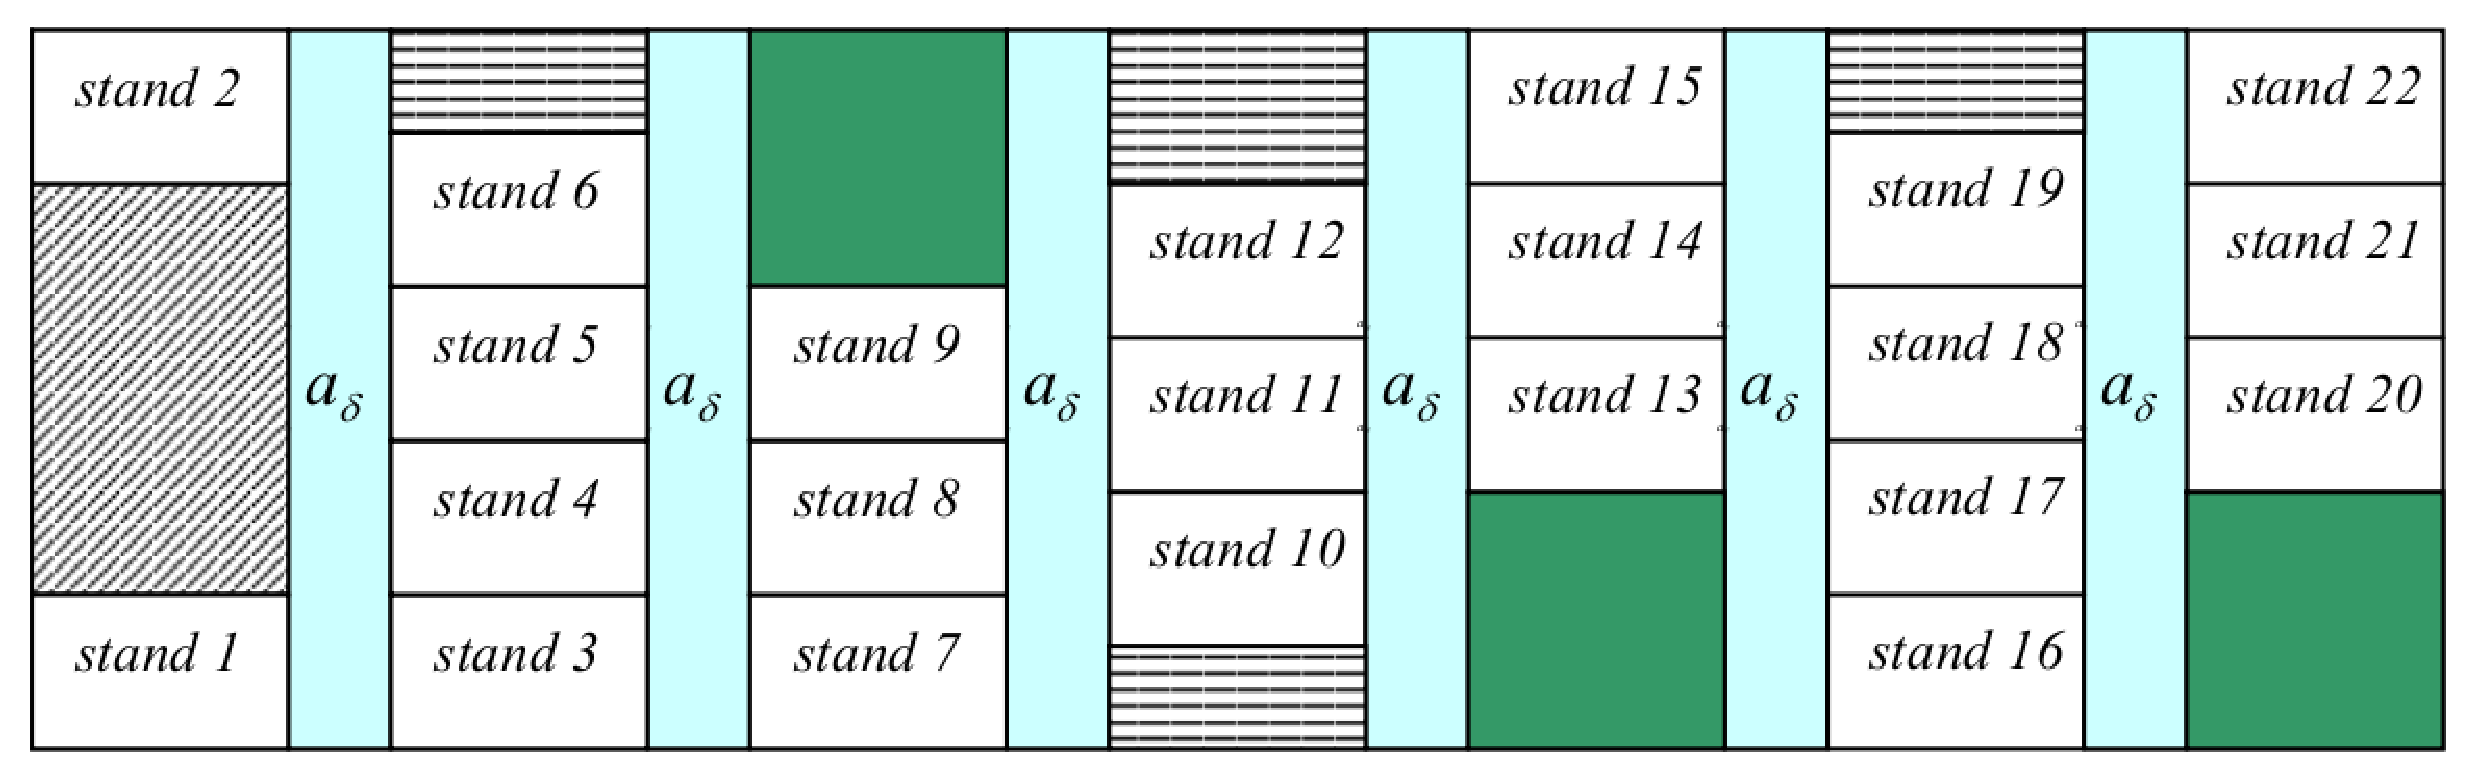
\includegraphics[width=13cm, height=5cm]{images/2strip.eps}
\textit{\caption{\footnotesize esempio di layout che tiene conto delle distanze tra le aisles per i pedoni e tra strips ($a_{\delta}$). Gli spazi colorati indicano zone in cui non risulta possibile posizionare stand.}}
\end{figure}  
\begin{figure}[h]
\centering
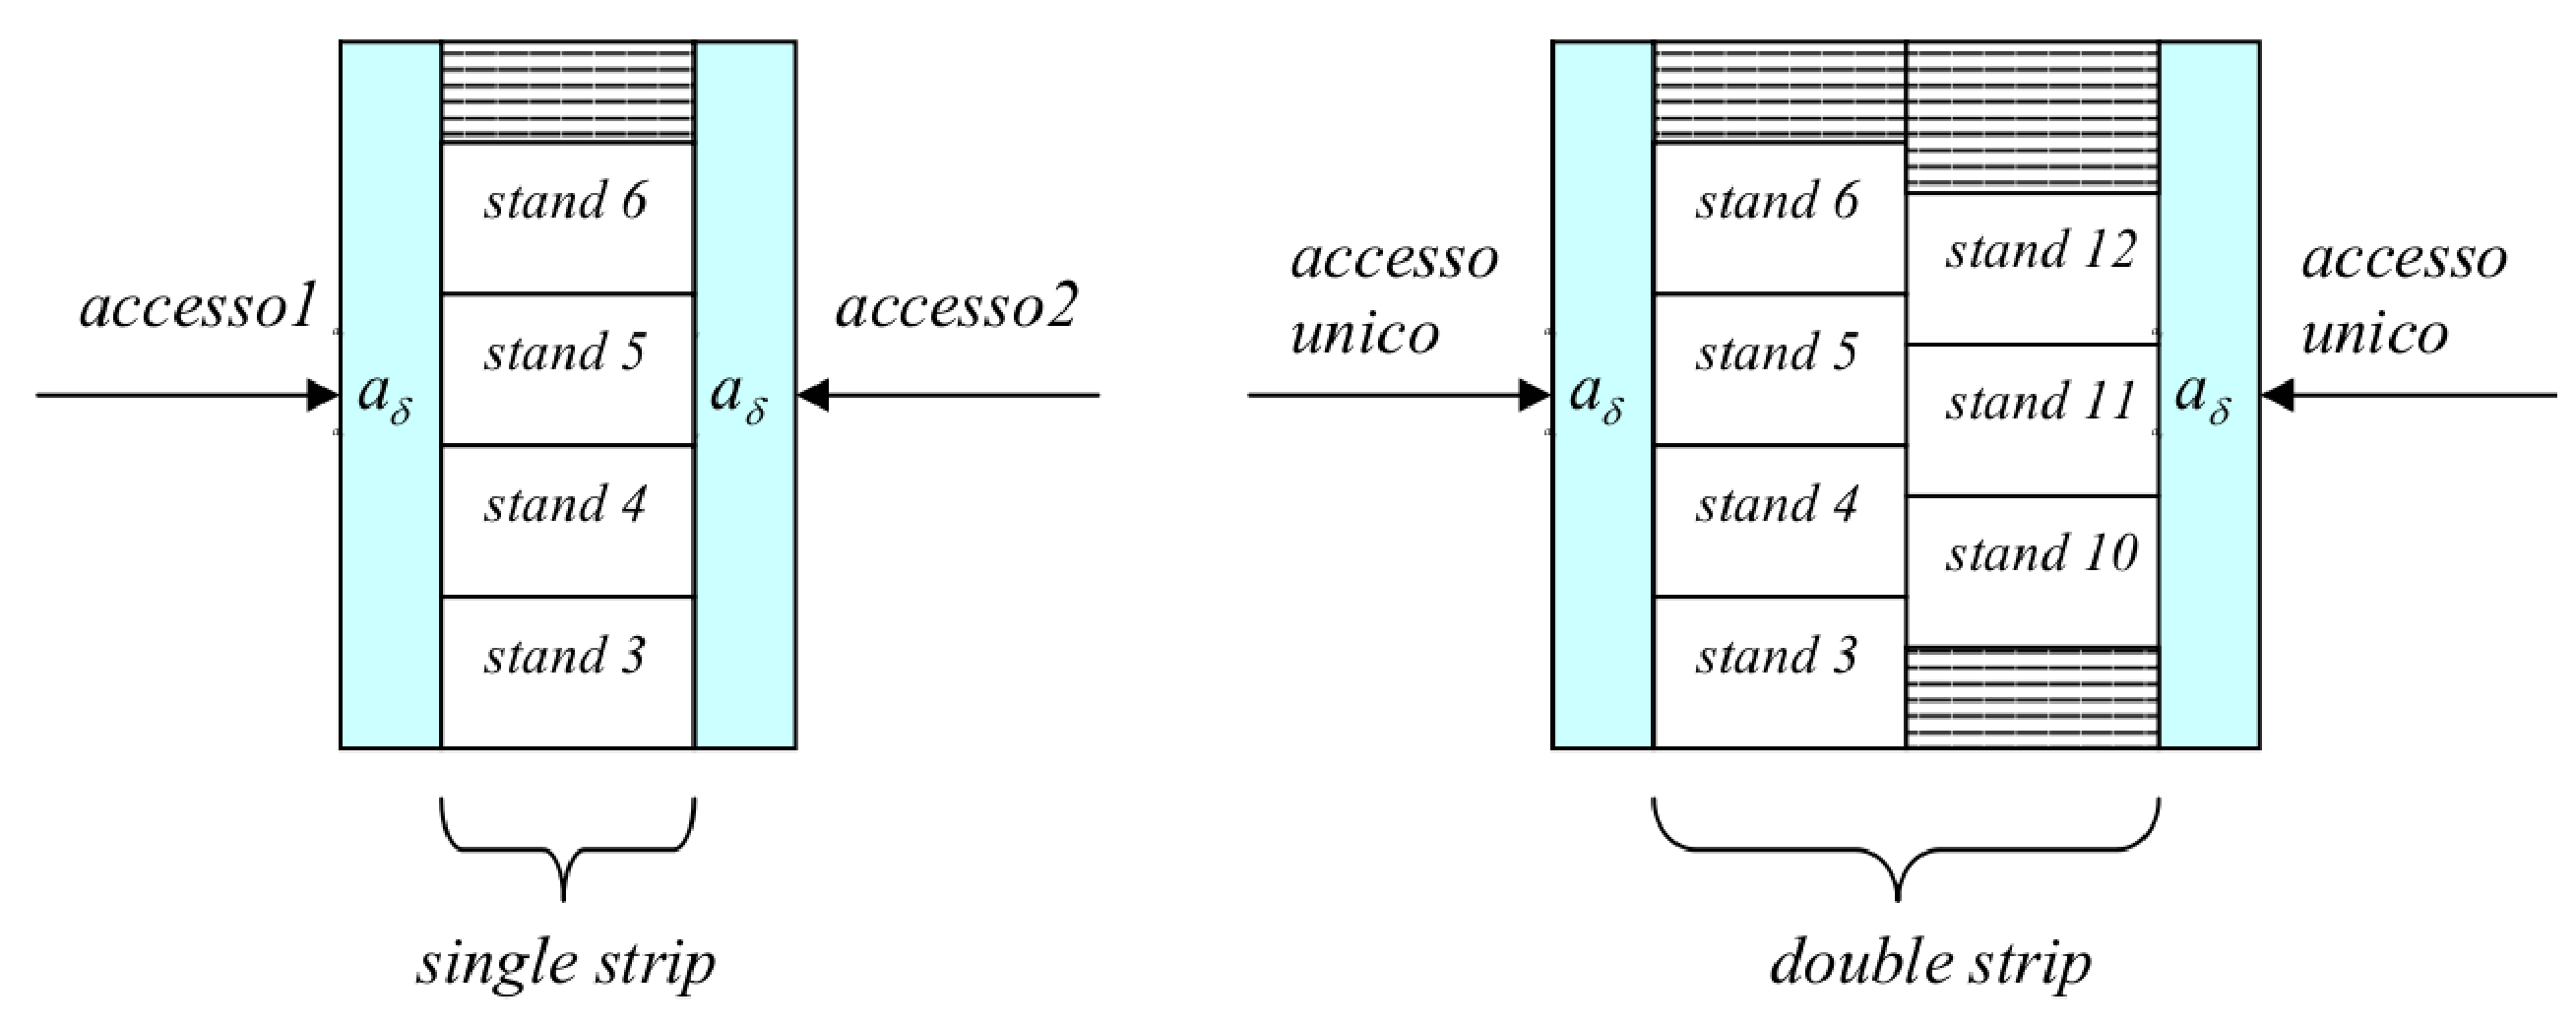
\includegraphics[width=12cm, height=5cm]{images/2strip_2.eps}
\textit{\caption{\footnotesize differenze tra FLOP1 e FLOP2: nel primo caso ogni stand ha due accessi e vi sono strip singole; nel secondo caso ogni dtand ha un solo lato di accesso libero ed \`{e} disposto su striscie doppie.}}
\end{figure} 
\\Infine, analizzando le due alternative presentate, si deduce una fondamentale propriet\`{a}:
\begin{quotation}
le matrici dei vincoli di tutte e due le varianti sono totalmente \textit{unimodulari};
\end{quotation}
dove per "`"`matrice unimodulare"'"' si intende una matrice $A$ che soddisfi i seguenti requisiti:
\begin{itemize}
\item $a_{ij} \in \left\lbrace -1, 0, 1\right\rbrace$
\item ciascuna colonna non deve avere pi\`{u} di due elementi non nulli
\item esiste una partizione ($A_{1}, A_{2}$) delle righe tale che per ogni colonna con due elementi non nulli, questi appartengono uno a $A_{1}$, e l'altro ad $A_{2}$ se e solo se sono concordi in segno
\end{itemize}
Se chiamiamo $A$ la matrice associata al vincolo (\ref{eq3}) si pu\`{o} facilmente constatare che $A$ \`{e} proprio \textit{unimodulare}: i coefficienti di ogni riga $i$ (sempre riferendosi ai constraint (\ref{eq3})) sono tutti zero tranne un insieme di $w+a$ valori unitari consecutivi che partono proprio da $i$. Questo insieme di elementi unitari \`{e} un gruppo di elementi $w_{\delta}$, ossia di larghezza $w$ e unit\`{a} di misura $\delta \thickapprox 20cm$ (in generale).
Ora sia $a^{'}_{i}$ il vettore associato alla riga $i$ di $A$, per $i = 1, ..., W-w+1$, e si modifichi $A$ ponga $a^{'}_{i} = a^{'}_{i} - a^{'}_{i+1}$, per $i=1,..., W - w +1$. In questo modo, partendo da $A$ si ottiene la matrice $\tilde{A}$ di Figura 2.7.
E' facile notare che la matrice $A$ soddisfa le condizioni sufficienti per essere una matrice totalmente unimodulare. In particolare la colonna avente pi\`{u} di due elementi non nulli pu\`{o} essere divisa in $A1 = A$ e $A2 = \oslash$.
\begin{figure}[h]
\centering
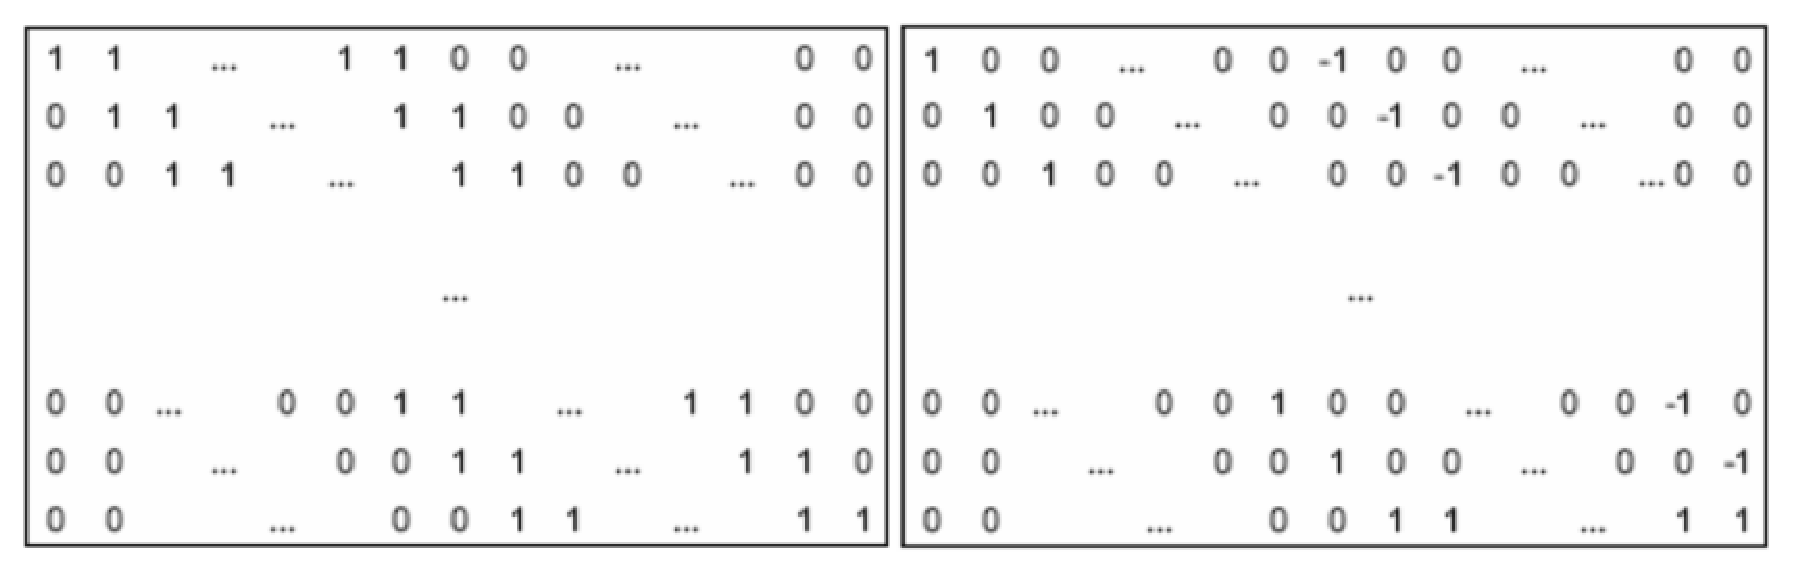
\includegraphics[width=12cm, height=4cm]{images/matrix.eps}
\textit{\caption{\footnotesize a sinistra, la matrice $A$ associata ai vincoli imposti dalla equazione (\ref{eq3}); a destra, la matrice $\tilde{A}$ ottenuta mediante alcune operazioni lineari sulle righe di $A$.}}
\end{figure}
Da ci\`{o} segue che entrambi i problemi FLOP1 e FLOP2 possono essere risolti in un \textit{polynomial time}\footnote{si fa riferimento a un problema risolvibile in tempi computazionali, mediante l'associazione della complessit\`{a} del problema a una funzione polinomiale} sostituendo i vincoli (\ref{eq4}) (corrispondenti ai vicoli (\ref{eq7})) e i vincoli (\ref{eq8})  con i loro rispettivi rilassamenti lineari:
$$ 0 \leq x_{j} \leq 1 \mbox{ , } (j = 1,...,W-w+1)$$
$$ 0 \leq \xi_{j} \leq 1 \mbox{ , } (j = 1,...,W-2w+1)$$
e risolvendo il risultante problema di programmazione lineare dato dalle (\ref{eq2}),(\ref{eq3}), (rispettivamente (\ref{eq7}) e (\ref{eq8})) insieme alle ultime due relazioni appena ricavate. 

\section{Studio e analisi di casi reali}
Nei prossimi due sottoparagrafi verranno presentate due metodologie di applicazione degli algoritmi per il layout fieristico. In particolare verranno analizzati i contesti della fiera dell'artigianato di Fortaleza (Brasile) sul lungomare di Beira Mar, e la fiera regionale di Romont (Svizzera), che ospita circa 100 espositori e 50 mila visitatori l'anno.
Tali contesti rappresentano un'analisi completa sotto i vari punti di vista, poich\'{e} coprono nel complesso tutte le possibilit\`{a} e le eventualit\`{a} che si possono presentare in ambito fieristico.
Se nel primo caso, infatti, si tratta di una fiera permanente, con sede su una superficie irregolare e suggestiva come la spiaggia del lungomare accanto a hotel, ristoranti e luoghi di turismo molto affollati, nel secondo caso si ha a che fare con una fiera regionale che ha luogo ogni due anni nella localit\`{a} di Romont, nel tipico paesaggio montuoso della Svizzera.\\
Due tipologie di studio piuttosto diverse, ma che coprono gran parte delle caratteristiche tipiche del contesto, in modo da poter far fronte ad un largo insieme di specifiche, requisiti e vincoli, al fine di creare un progetto completo e adeguato ad ogni evenienza.

\subsection{Caso 1: Fortaleza handcraft fair}
Ogni giorno circa seicento artigiani si recano all'altezza della spiaggia di Meireles e assemblano e smontano i loro stand per dare vita                                                                   a una famosa fiera di artigianato che da anni \`{e} presente sul lungomare di Fortaleza (Brasile).\\
L'area che circonda la fiera \`{e} una delle zone pi\`{u} attive della citt\`{a} ed \`{e} piena di noti hotel e ristoranti. E' stata l'importanza di questa fiera, data dal grande numero di persone che vi lavorano e dall'enorme affluenza di visitatori, e la complessit\`{a} dell'ambiente entro cui essa \`{e} collocata, che hanno spinto l'Universit\`{a} di Cear\'{a} a trasformare la disposizione degli stand dei cosiddetti \textit{Juarez} in un vero e proprio problema di ottimizzazione. Questo grande ammontare di stand ha infatti bisogno di una disposizione meno caotica e pi\`{u} razionale che renda possibile l'inserimento di pi\`{u} artigiani possibile.\\
Lo scopo della ricerca consiste quindi nel massimizzare il numero di stand che possono essere contenuti nella superficie adibita alla fiera, cercando di ottenere un layout accettabile, ovvero un layout che consideri anche tutti gli spazi necessari per il passaggio delle persone e per il montaggio/smontaggio degli stand. Tutto ci\`{o} tenendo ben presente che la superficie disponibile per l'esposizione \`{e} di forma irregolare e non convessa (all'interno e attorno alla superficie sono infatti presenti numerosi ostacoli: palme, sculture, panchine..) e che gli stand sono tutti uguali e rettangolari. Proprio queste ultime considerazioni, rendono il problema generalizzabile ad ogni altro contesto
fieristico e quindi particolarmente interessante.
\begin{figure}[h]
\centering
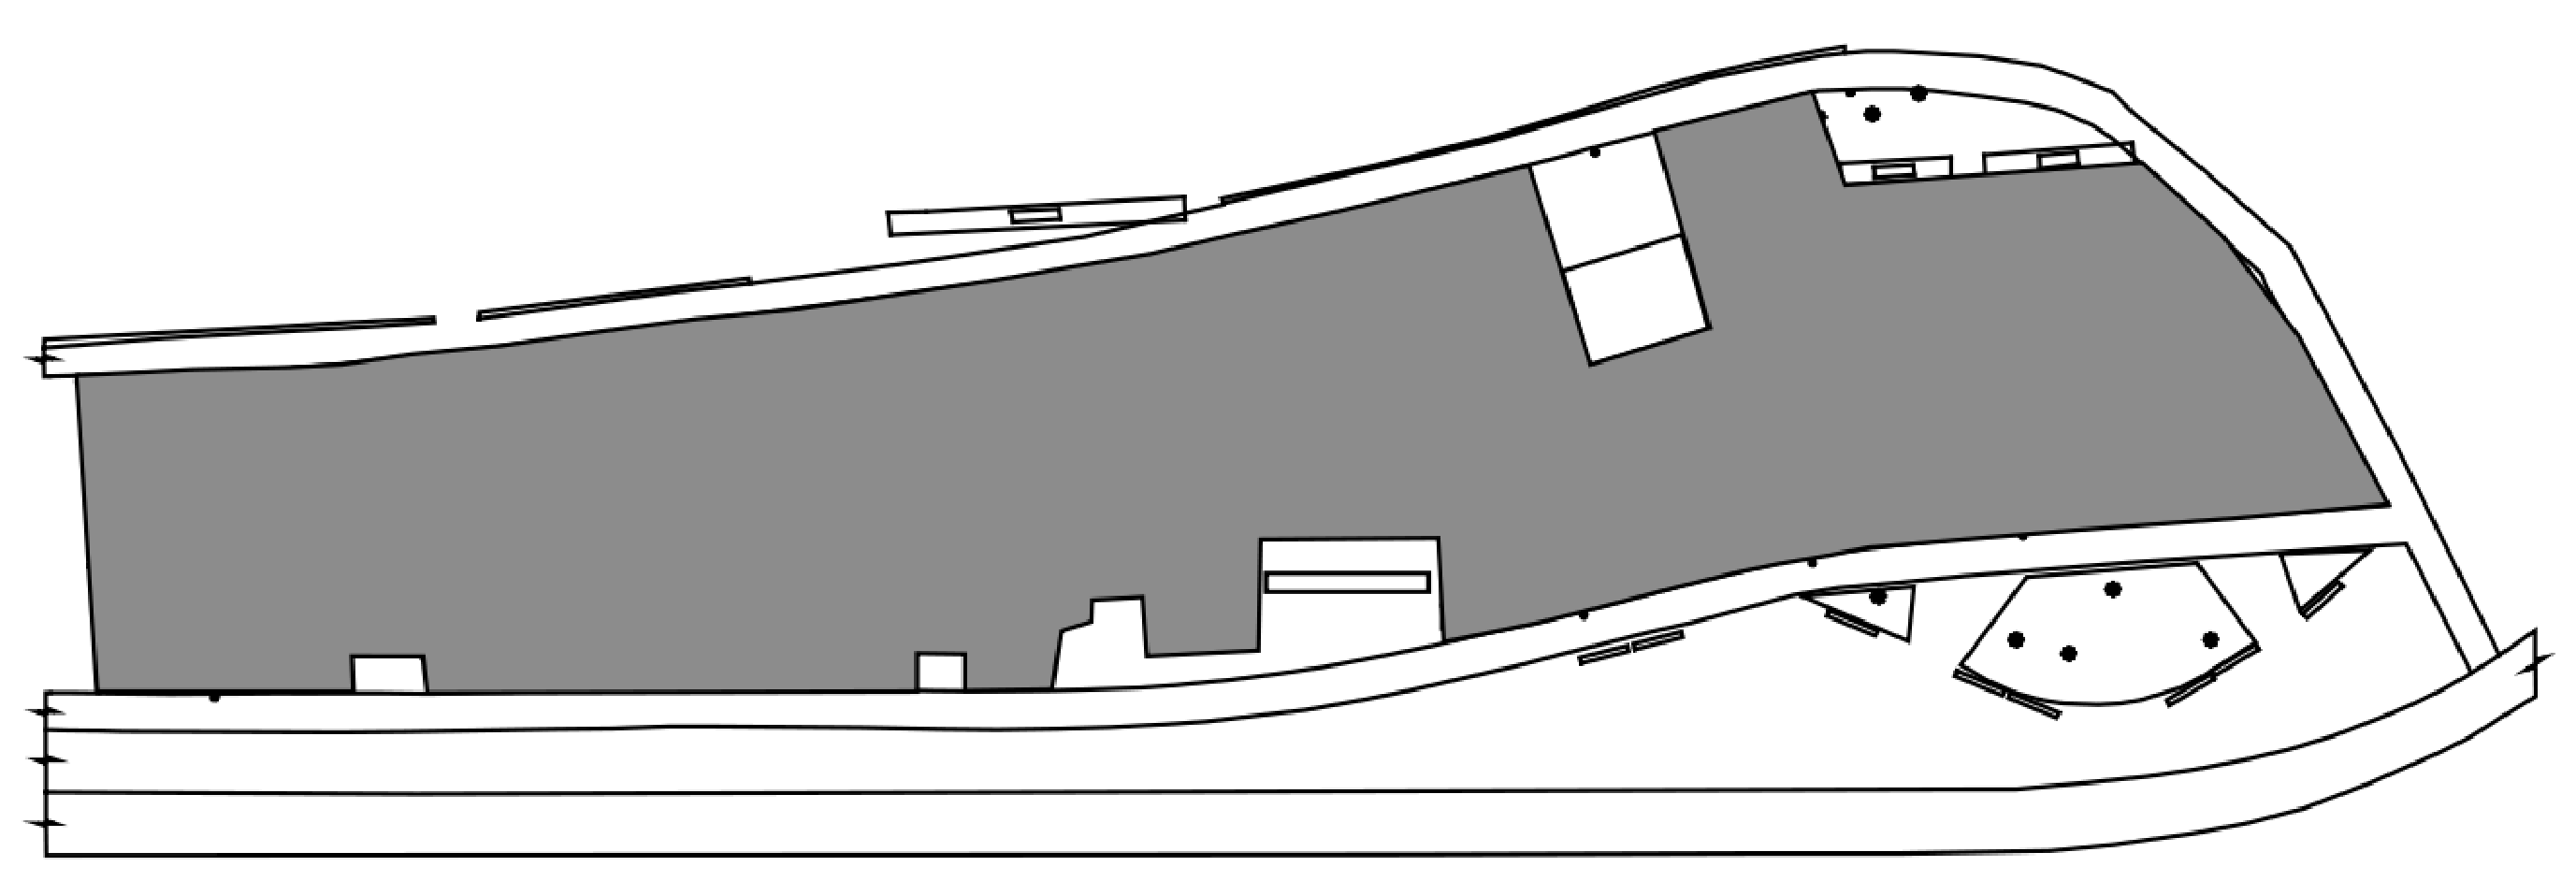
\includegraphics[width=12cm, height=4cm]{images/fortaleza1.eps}
\textit{\caption{\footnotesize vista dall'alto della zona dedicata all'esposizione fieristica (indicata in grigio) in localit\`{a} Beira Mar, a Fortaleza}}
\end{figure}
\\In figura 2.8 \`{e} disponibile una piantina che ritrae la superficie di esposizione della fiera di Fortaleza.   \\
L'algoritmo corrispondente al problema di programmazione lineare della fiera \`{e} stato implementato utilizzando un software free dotato di interfaccia grafica semplice e intuitiva che potesse permettere di facilitare le operazioni di disegno del layout\footnote{tutte le simulazioni e i test sono stati eseguiti su macchine con processore Pentium 4 a 1.8GHz dotate di 2GB di RAM.}.\\
Le dimensioni dell'area che ospita il layout sono circa di 200 metri di larghezza (che indichiamo, coerentemente con quanto visto nelle sezioni precedenti con $W$) e 50 metri di altezza (che indichiamo con quindi con $H$). L'analisi, risalente al 2006, conta 617 stands, posizionati in 26 striscie doppie, con arrangiamento piuttosto simile a quello pensato per il FLOP2, mentre per quanto riguarda l'altezza e la larghezza degli stand, vale per tutti $h = 2$ e $w = 2$ metri. E' importante sottolineare che che l'area \`{e} di tipo non convesso, ossia c'\`{e} la presenza di alberi, piccoli negozietti, lampioni, monumenti, per cui alcune aree non sono disponibili per l'installazione di stands.
Nel caso in questione, definendo $\delta = 5cm$ si ottengono $w = h = 40$, $W = 4090$ e $H = 1084$; il valore indicativo fornito per determinare la larghezza del passaggio pedonale (\textit{aisle}) \`{e} di $3.5m$, ovvero $a = 70$.\\
I passi effettuati per testare l'efficienza degli algoritmi FLOP1 e FLOP2 consistono in operazioni piuttosto complicate e laboriose, soprattutto nel passare dalla mappatura reale a quella virtuale (per lo scopo sono stati utilizzati strumenti di CAD) e per convertire il tutto in formato SHP\footnote{shapefile, formato vettoriale per sistemi informativi geografici che traduce le informazioni grafiche in dati geometrici ricchi di attributi di corredo alle forme poligonali che determinano le elaborazioni} contenente le "`"`georeferenze"'"' e le coordinate della superficie espositiva. A sua volta il file SHP \`{e} stato convertito in una matrice bineria $M$ di dimensione $1084 \times 4090$ (comune ai due modelli), mediante un programma chiamato Delphi Object Pascal\footnote{della software house "`"`Borland"'"'}; questa conversione ha richiesto un tempo computazionale molto lungo, circa 1000 secondi di elaborazione da parte della CPU.
\begin{figure}[h]
\centering
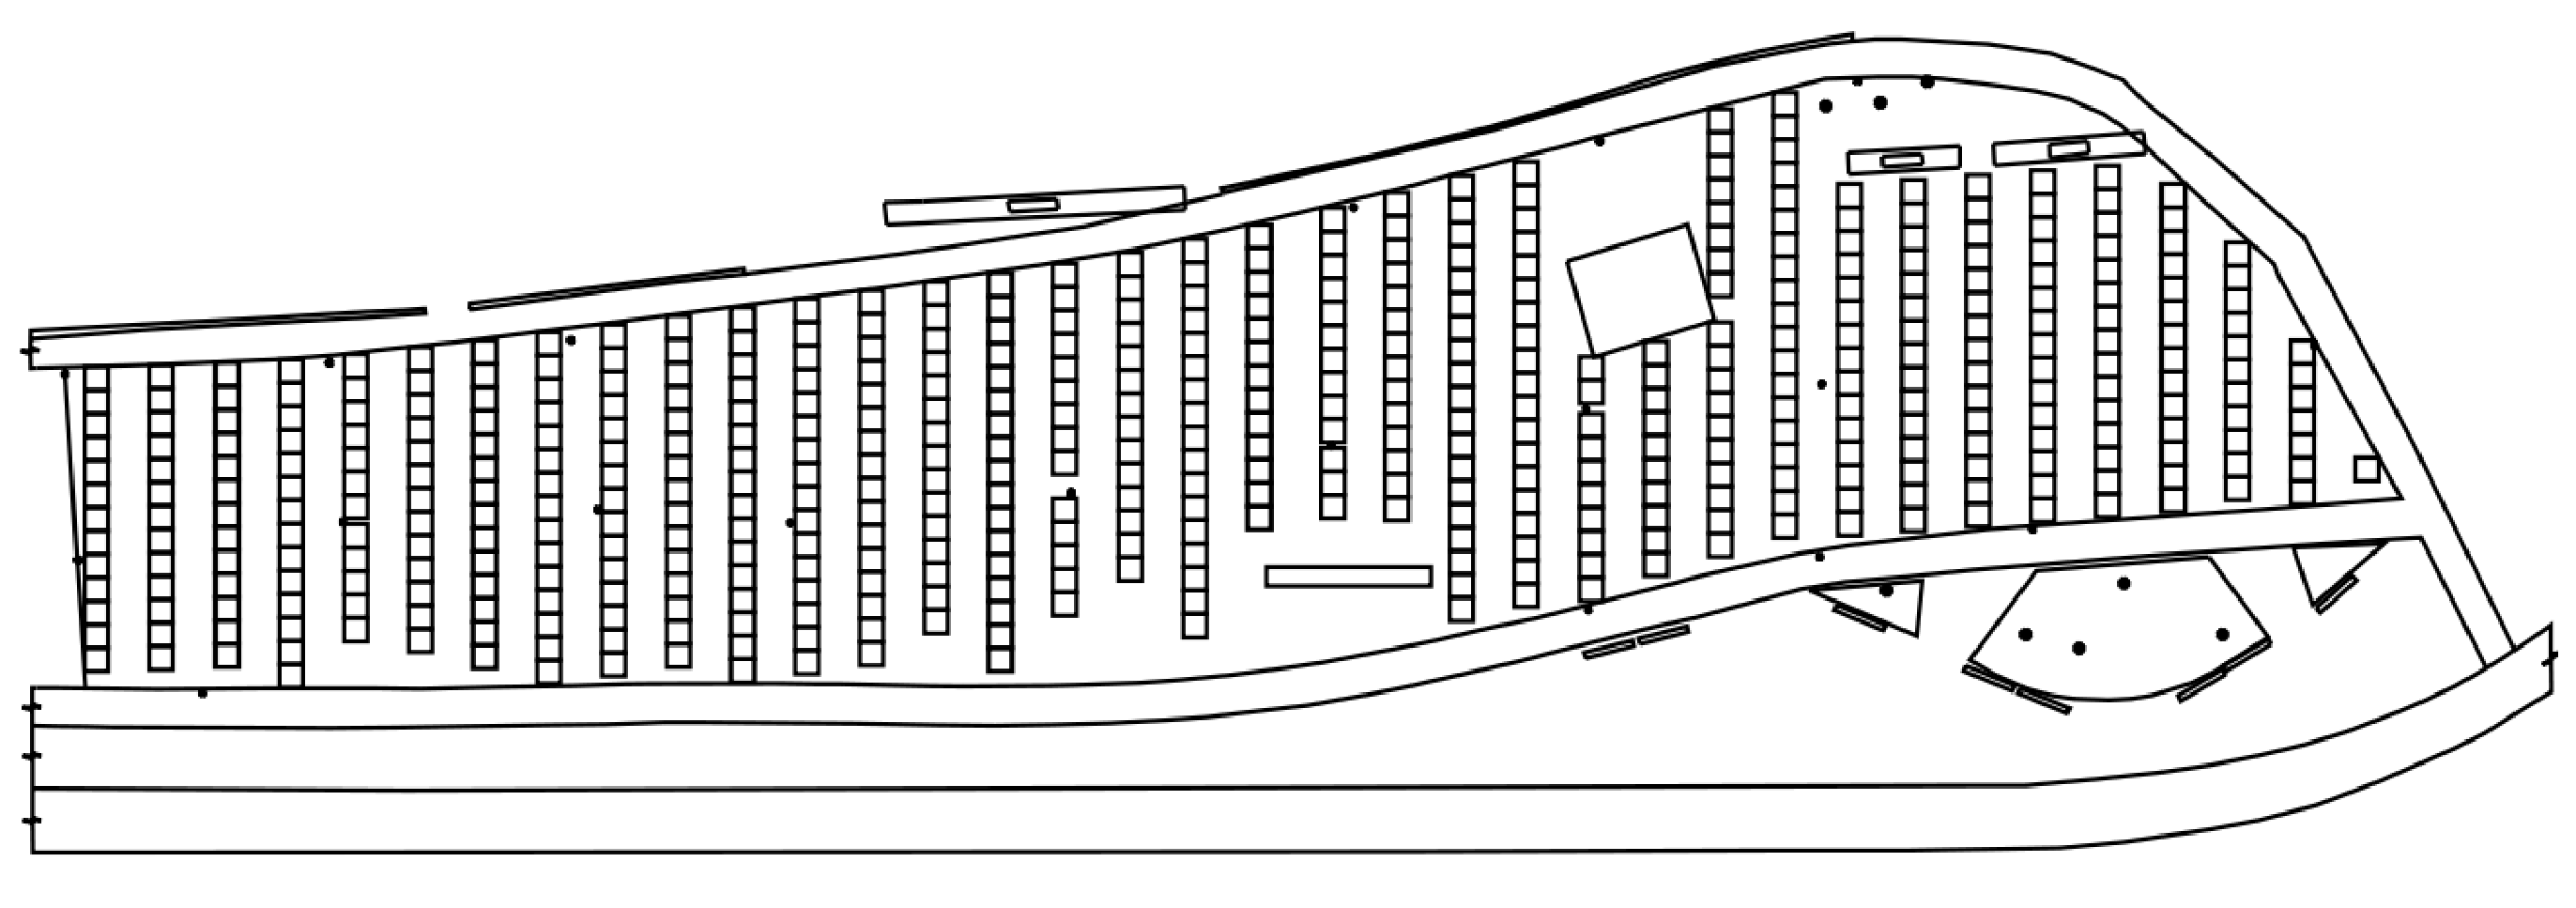
\includegraphics[width=12cm, height=4cm]{images/fortaleza2.eps}
\textit{\caption{\footnotesize output relativo alla soluzione mediante algoritmo FLOP1.}}
\end{figure}
\begin{figure}[h]
\centering
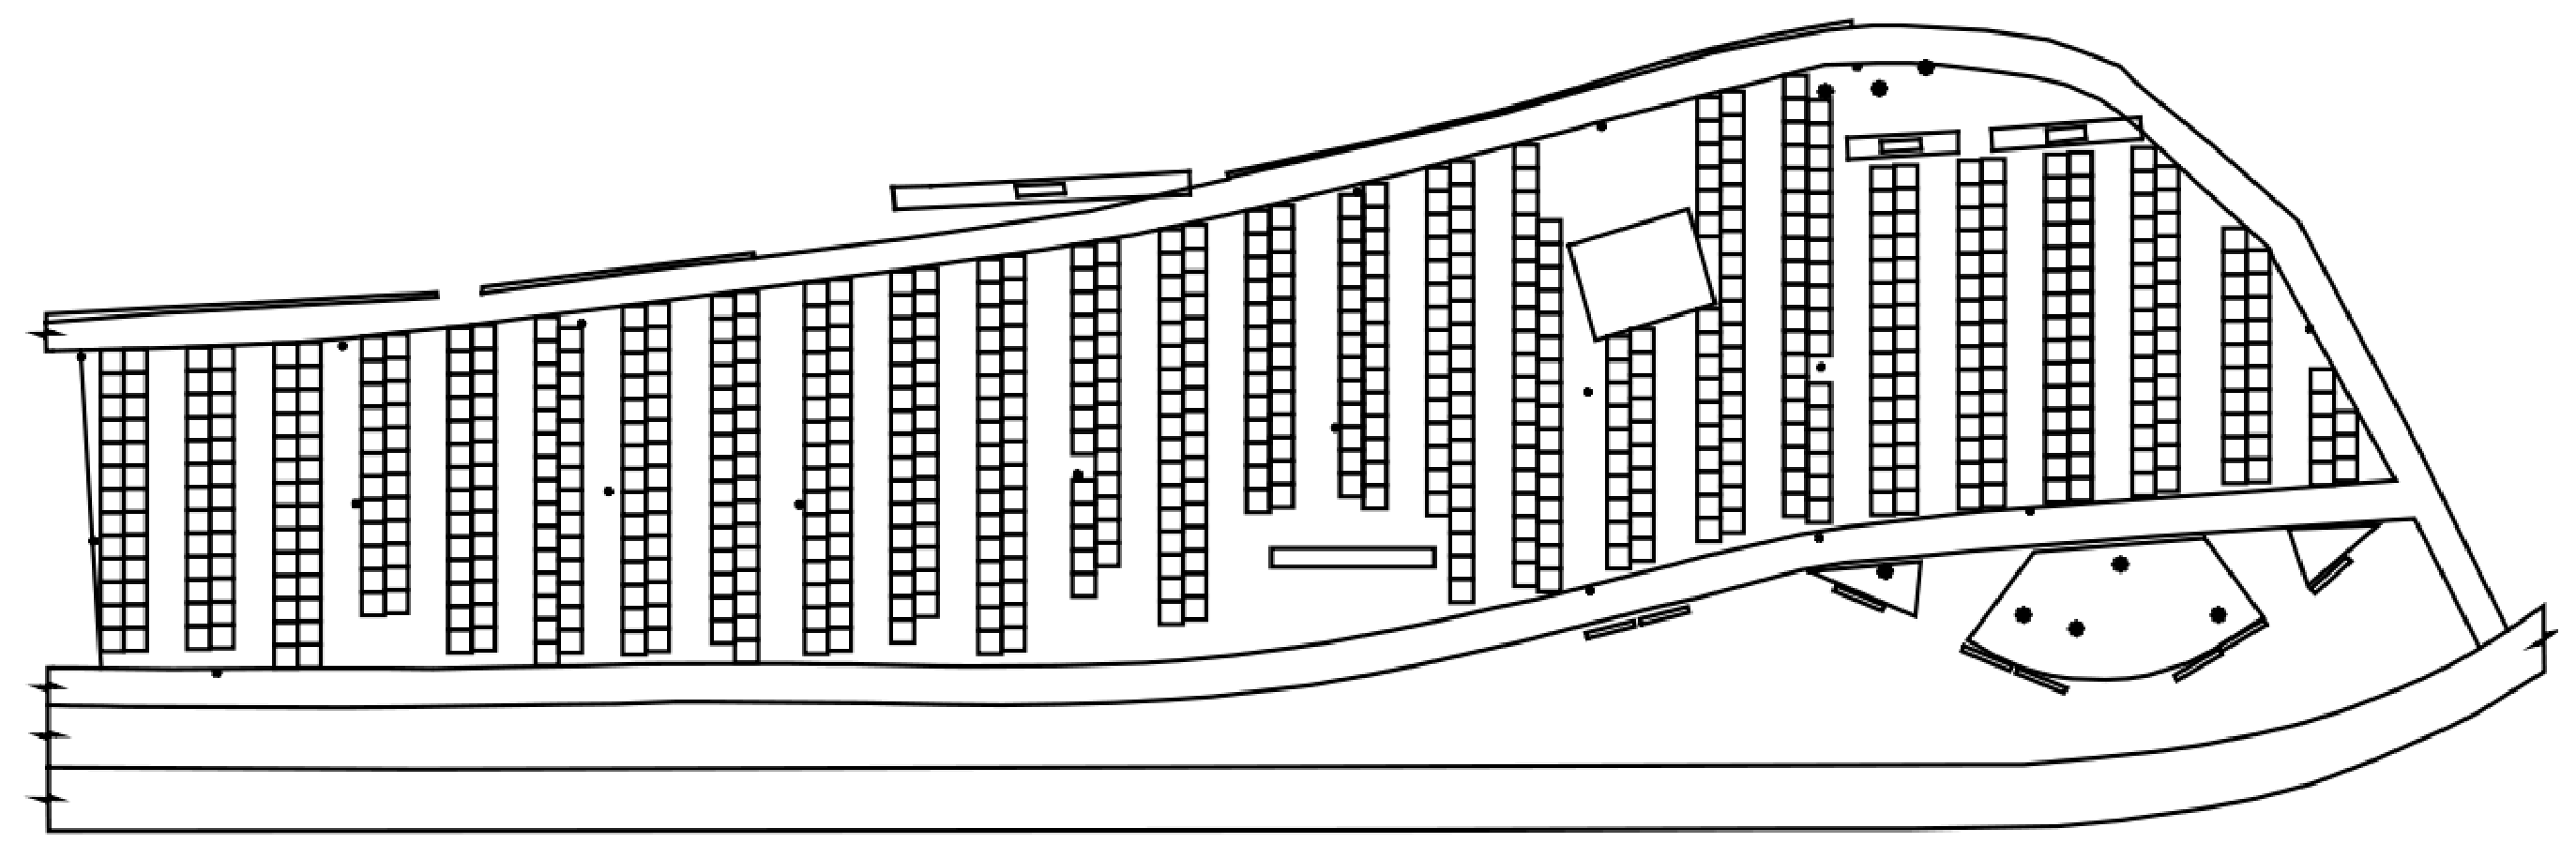
\includegraphics[width=12cm, height=4cm]{images/fortaleza3.eps}
\textit{\caption{\footnotesize output relativo alla soluzione mediante algoritmo FLOP2.}}
\end{figure}
\\Il modello FLOP1, la cui soluzione \`{e} rappresentata il figura 2.9, \`{e} stato elaborato e risolto in 24 secondi e la soluzione ottimizzata ha fornito come output un totale di 505 stands disposti su 36 file singole (le \textit{strips}) con meno del 20\% di decremento rispetto al caso di partenza (a striscie doppie). Il modello FLOP2, invece, \`{e} stato risolto dal software in 62 secondi e la soluzione, in figura 2.10, ha calcolato 742 stands arrangiati in 26 \textit{double strips}, incrementando del 20\% la soluzione di partenza.\\
Stando ad esigenze ulteriormente stringenti, alcuni organizzatori hanno richiesto anche di sfruttare la zona in alto a destra (di forma grosso modo triangolare) e si sono ottenute altre soluzioni, impiegando 759 stands sempre su 26 striscie doppie (quindi sempre riferendosi al FLOP2). Nessuna delle soluzioni proposte dal FLOP2 ha avuto modo di combinarsi con quelle proposte dal FLOP1 e cio\'{e} non vi \`{e} modo di combinare striscie singole e doppie, probabimente a causa del fatto che le \textit{aisles} pedonali sono relativamente piuttosto larghe, e non conviene uscire dalle alternative trovate.\\
Una ulteriore possibilit\`{a} per ottimizzare ancora di pi\`{u} le prestazioni computazionali consiste nel cambiare i valori di $\delta$, che non ottimizzano le questioni di spazio, ma di tempo. Ad esempio per $\delta = 10cm$ l'algoritmo ha bisogno di 246 secondi per costruire la matrice $M$, di 4 secondi per risolvere il FLOP1 e di 10 secondi per quanto riguarda il FLOP2. Inoltre, nel primo caso si contano 503 stands invece che 505, mentre per il FLOP2 si hanno gli stessi 742 stands che in precedenza. Per $\delta = 20cm$ si hanno 64 secondi per costruire la matrice, e 2 secondi per FLOP1 e 1 secondo per FLOP2 con un ulteriore decremento degli stands, rispettivamente a 499 e 737. Per valori sempre pi\`{u} piccoli di $\delta$, fino a $\delta=5cm$, si sono ottenuti tempi di calcolo empre pi\`{u} elevati, senza per\`{o} alcun beneficio in ottimizzazione.\\
\\Il campo che interessa i layout fieristici ha assunto notevole importanza soprattutto negli ultimi anni, ed  \`{e} diventato di fondamentale importanza in materie come la Ricerca Operativa e in applicazioni matematiche e informatiche. Tuttavia \`{e} un problema in piena evoluzione e in continua fase di studio per l'ottimizzazione combinatoria, perci\`{o} come tale richiede continui adattamenti e revisioni in modo da poter soddisfare un numero sempre pi\`{u} ampio di requisiti e coprire in larga scala tutte le eventualit\`{a}.
A titolo di esempio si consideri propio il caso di Fortaleza, in cui gli organizzatori hanno proposto nuove alternative e introdotto nuove \textit{constraints} al problema: nel caso appena analizzato, una delle specifiche consisteva nell'arrangiare le strips in modo perpendicolare alla spiaggia (la base della piantina); ma \`{e} possibile "`"`comporre"'"' gli stands in altro modo, producendo soluzioni migliori o adatte alle varie esigenze che cambiano di volta in volta. Considerando un approccio tipico dei layout generici, non sarebbe insensato disporre gli stands a gruppi di 4, come rappresentato in figura 2.11.\\
\begin{figure}[h]
\centering
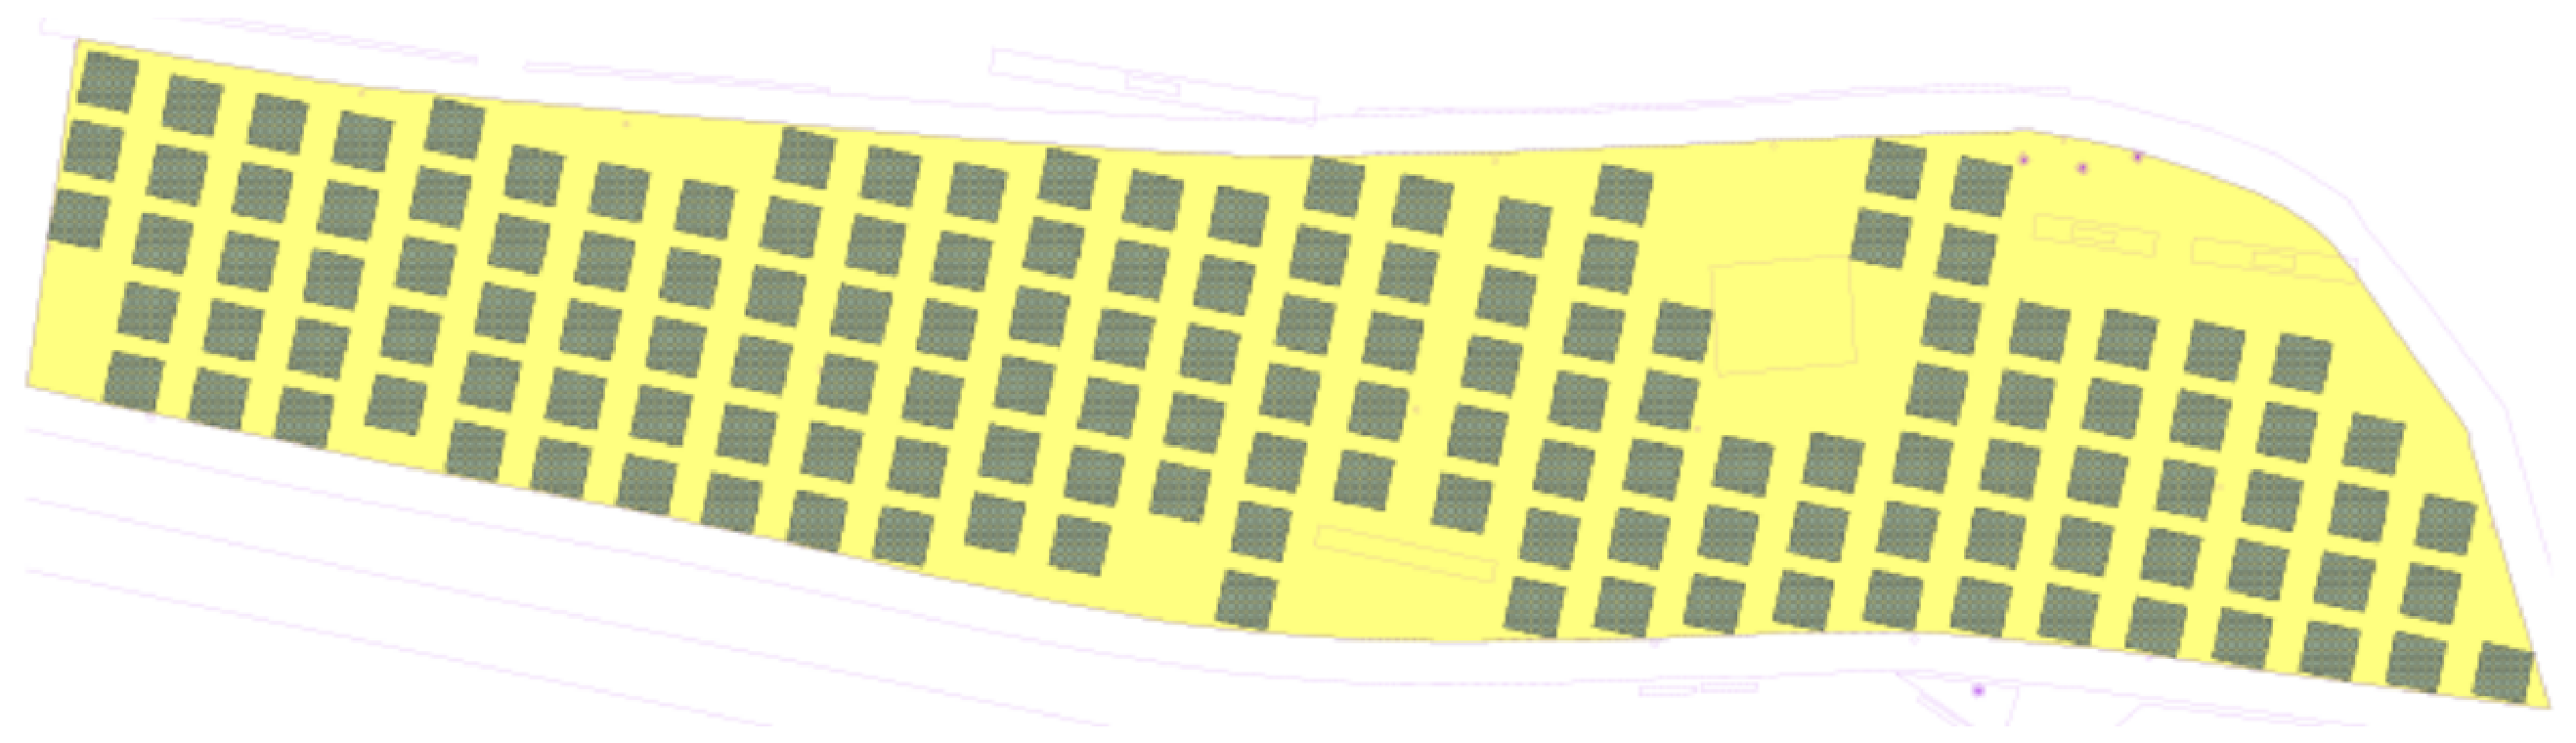
\includegraphics[width=12.5cm, height=4cm]{images/fortaleza4.eps}
\textit{\caption{\footnotesize bozza alternativa alle varianti previste per la soluzione; si dispongono gli stands a gruppetti di quattro.}}
\end{figure} 

\subsection{Caso 2: Regional fair in Romont}
La fiera regionale di Romont ha luogo ogni due anni in un paese di 4 mila abitanti circa, a met\`{a} strada tra Ginevra e Berna, nella Svizzera francofona. La zona adibita alle esposizioni \`{e} di circa 5200 mq (le dimensioni precise sono di $W = 100$ metri di lunghezza e $H = 52$ metri di larghezza del rettangolo) e al suo interno si presentano merci e servizi di almeno un centinaio di espositori.
Nel 1998 si sono registrati circa 50 mila visitatori durante gli 8 giorni dedicati alla manifestazione. Sotto quest'ottica gli organizzatori hanno necessitato di provvedimenti per ottimizzare il layout e far fronte ad eventuali aumenti dei visitatori. Di solito, l'approccio utilizzato dall'organizzazione consiste nel partire da una lista degli espositori e delle loro richieste in termini di spazi, per poi adeguare il layout soddisfacendo un cliente alla volta; un approccio alternativo, invece, prevede di partire da un layout predefinito e di assegnare a ciascun espositore una superficie che ne soddisfi le esigenze.
\begin{figure}[h]
\centering
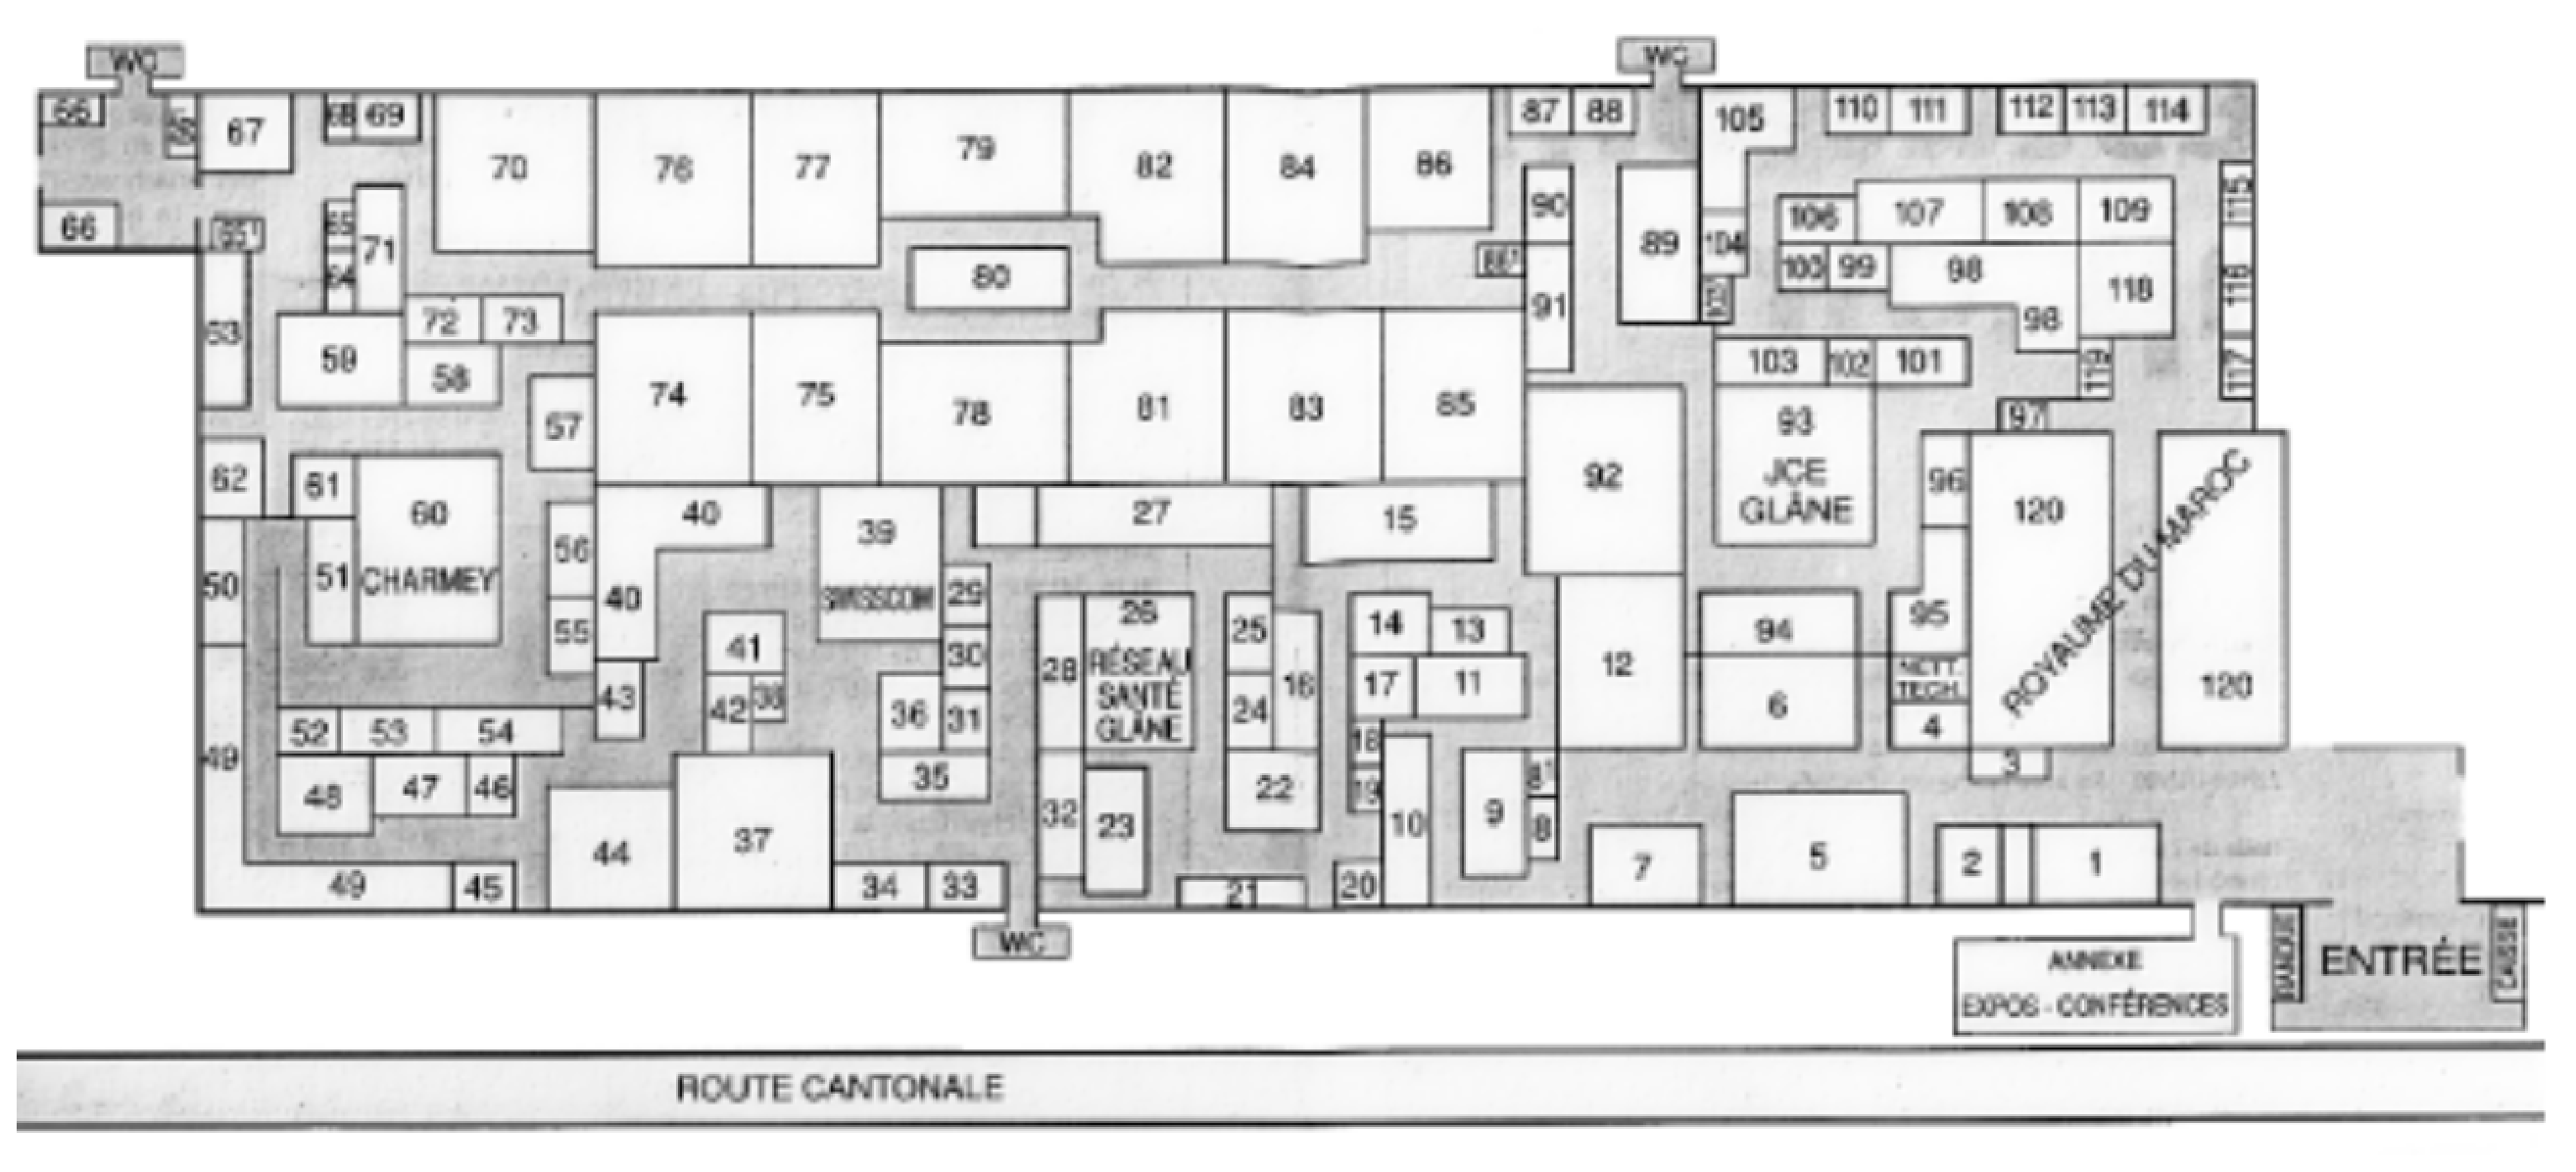
\includegraphics[width=12.5cm, height=5cm]{images/romont_high1.eps}
\textit{\caption{\footnotesize disposizione degli stands nell'edizione del 1998 della fiera.}}
\end{figure} 
\\Si pu\`{o} suddividere il processo di sviluppo delle soluzioni in due branchie: allocare in primis lo spazio per gli stands, in maniera tale da non sovrapporre gli spazi espositivi; in secondo luogo allocare gli spazi per il flusso dei visitatori (ci\`{o} che di solito indichiamo con \textit{aisles}). Vediamo in dettaglio questi due punti.
\begin{itemize}
\item Poich\'{e} una delle caratteristiche portanti della fiera di Romont \`{e} che non si mantiene tale e quale alle edizioni precedenti, i progettisti del layout devono ogni volta adattarsi alle nuove disposizioni ed esigenze e quindi riproporre ogni anno soluzioni diverse: il tutto si traduce in una raccolta di requisiti che comprende la prima parte del progetto. In particolare si raccolgono informazioni su:
\begin{itemize}
\item la forma e le dimensioni degli stands (se rettangolari o ad angolo\footnote{che possono essere piazzati in un angolo dell'area espositiva}, con le relative misure)
\item i lati di accesso agli stands
\end{itemize}
\item Il flusso di persone che pu\`{o} transitare all'interno degli spazi adibiti pu\`{o} essere elevato ed \`{e} quindi necessaria un'efficace affluenza nel percorso riservato alla clientela. La peculiarit\`{a} che si riscontra nella fiera di Romont sta nel fatto che il cliente deve seguire un percorso guidato e obbligato tra i vari stand, in modo da poterli visitare tutti\footnote{questa strategia \`{e} tipica anche in altri ambiti, quali ad esempio nei discount o in supermercati (vedi IKEA), ma \`{e} un caso piuttosto singolare quando si tratta di fiere regionali}. Nel caso in esame lo spazio dei corridoi va da un minimo di 2 metri ad un massimo di 3
\end{itemize}
In aggiunta a queste caratteristiche vanno aggiunti altri vincoli che sono rappresentati da ostacoli all'interno dello spazio, ossia presenza di bagni e toilettes, di muri, colonne e barriere architettoniche, di uscite d'emergenza, ecc., seppur comunque il carico di lavoro da affrontare si basa su tre fattori determinanti:
\begin{description}
\item[utilizzo degli spazi]: \`{e} l'aspetto pi\`{u} importante, dal quale derivano gli altri due. Si tratta dell'ottimizzazione di tutti gli spazi possibili, nel senso che ogni spazio inutilizzato (\textit{dead space}), va comunque "`"`reso utile"'"' e adibito agli stands
\item[valore attrattivo]: rappresenta la "`"`capacit\`{a}"'"' della fiera di attirare il maggior numero possibile di clienti e visitatori. Non dipende solamente da fattori quali marketing o promozioni, ma anche, e soprattutto, da un progetto accorto. Ciascuno stand deve avere una propria locazione il pi\`{u} attraente possibile: il caso ideale sarebbe di disporli in modo che l'\textit{open side} di ciascuno di essi si affacci sul percorso dei visitatori  
\item[agevolazioni ai visitatori]: naturalmente una qualsivoglia manifestazione, mostra o esposizione fieristica deve essere comoda da visitare e piacevole da vedere. Deve prevedere accorgimenti mirati alla comodit\`{a} del cliente in modo da invogliarne e stimolarne la curiosit\`{a}; bisogna quindi tenere conto dei percorsi (magari intervallando con aree di sosta e minimizzando i cambiamenti di direzione, per non affaticare la visita), degli spazi e del contesto in cui ci si trova 
\end{description}
\`{E} ovvio che risulta impossibile soddisfare appieno tutte e tre le specifiche, perci\`{o} occore cercare un trade-off tra di esse in modo da adeguare il progetto alle esigenze di organizzatori, espositori e visitatori. Generalmente tale compromesso dipende dall'abilit\`{a} e dall'esperienza del progettista.
\begin{figure}[h]
\centering
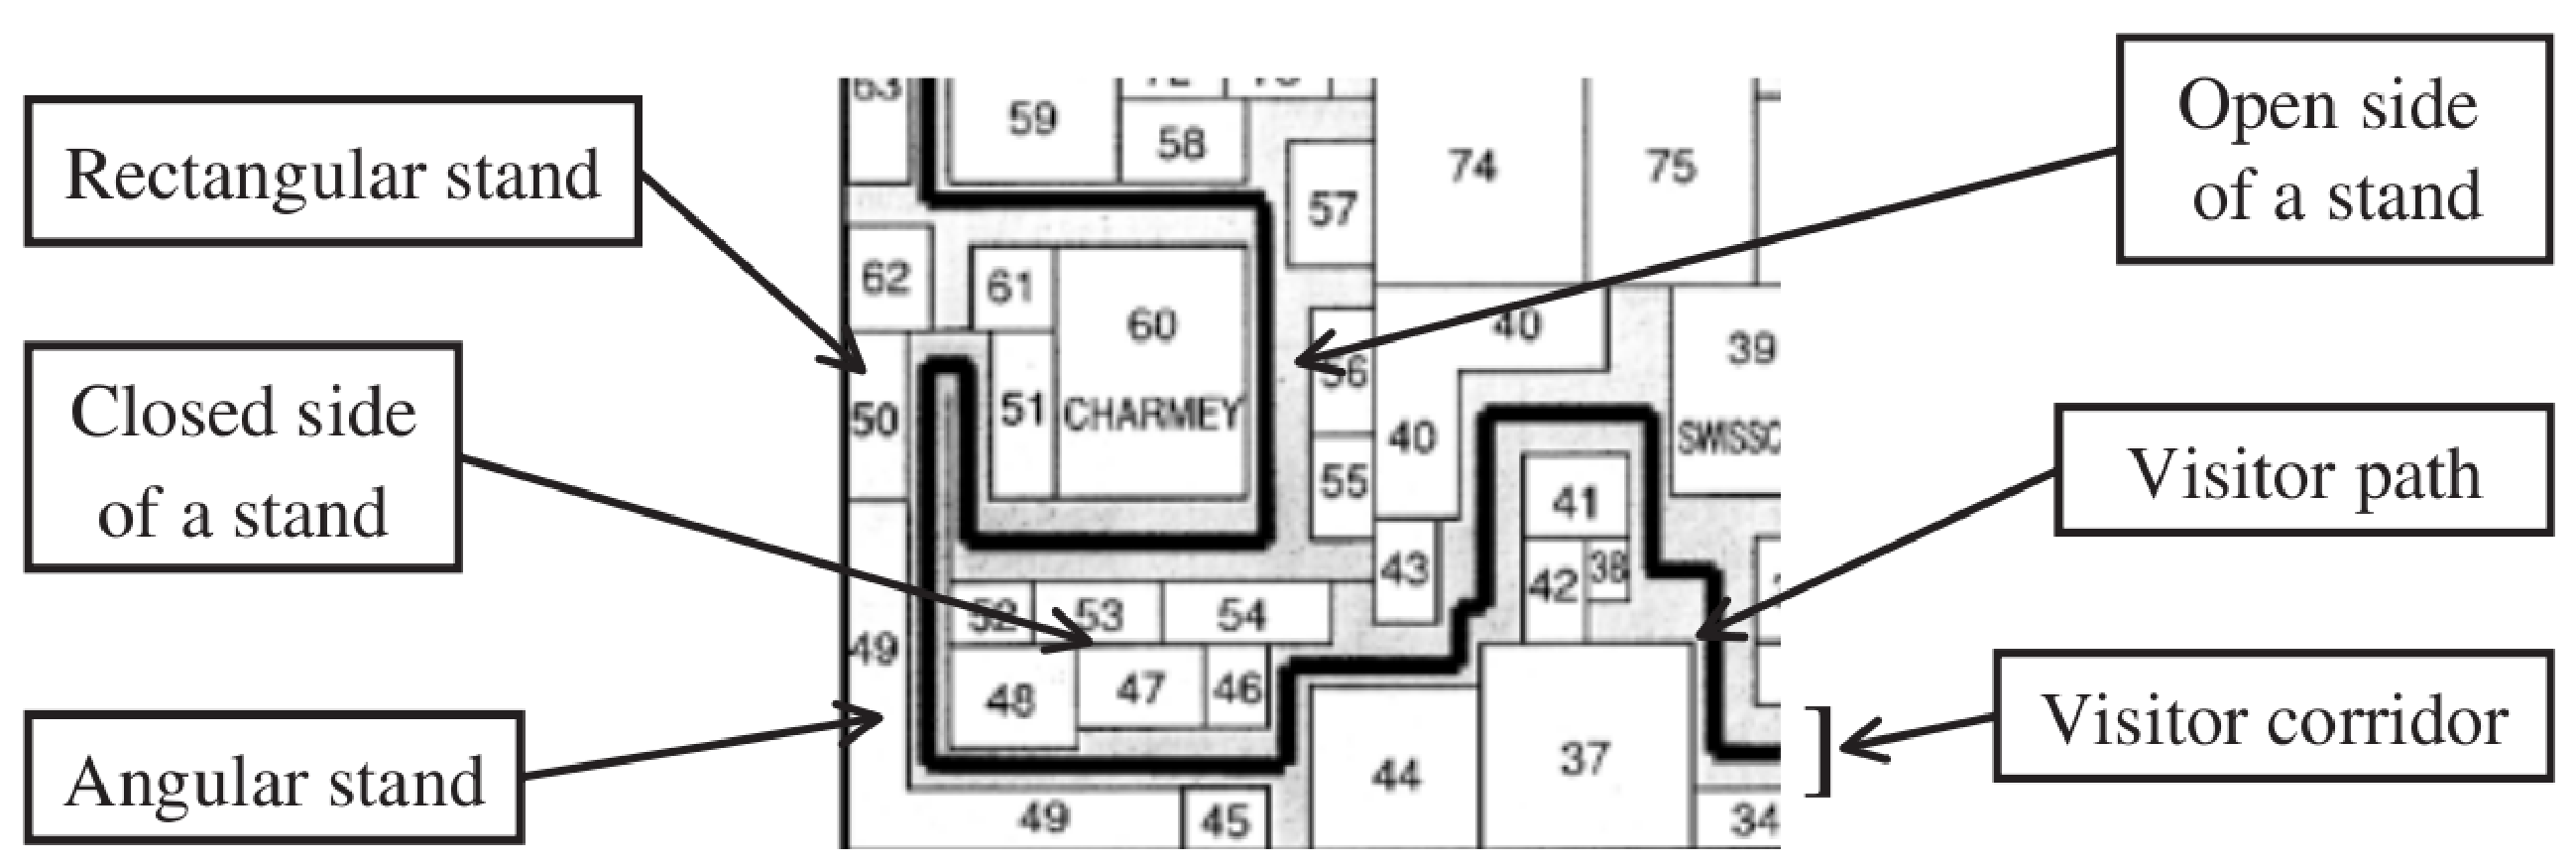
\includegraphics[width=12cm, height=4cm]{images/romont_stands.eps}
\textit{\caption{\footnotesize descrizione degli items utilizzati nel progetto e legenda.}}
\end{figure} 
\\Il modello cui ci si \`{e} attenuti nel progettare il layout \`{e} l'\textit{adjacency model}, che permette una rappresentazione basata sull'adiacenza del percorso dei visitatori ai lati aperti degli stand espositivi; viene usata una discretizzazione degli elementi coinvolti nel processo di layout e questo significa che la superficie e gli spazi richiesti sono espressi come valori interi e multipli dell'unit\`{a} base dell'area, mentre la superficie espositiva \`{e} associata ad un rettangolo suddiviso in alcune unit\`{a} di misura di base, come si pu\`{o} vedere dalle figure seguenti. In particolare la lunghezza del rettangolo \`{e} di $L$ unit\`{a}, mentre la altezza \`{e} $B$ unit\`{a}. 
Ogni punto all'interno del rettangolo pu\`{o} essere identificato mediante le coordinate sugli assi cartesiani come illustrato in figura 2.14.
\begin{figure}[h]
\centering
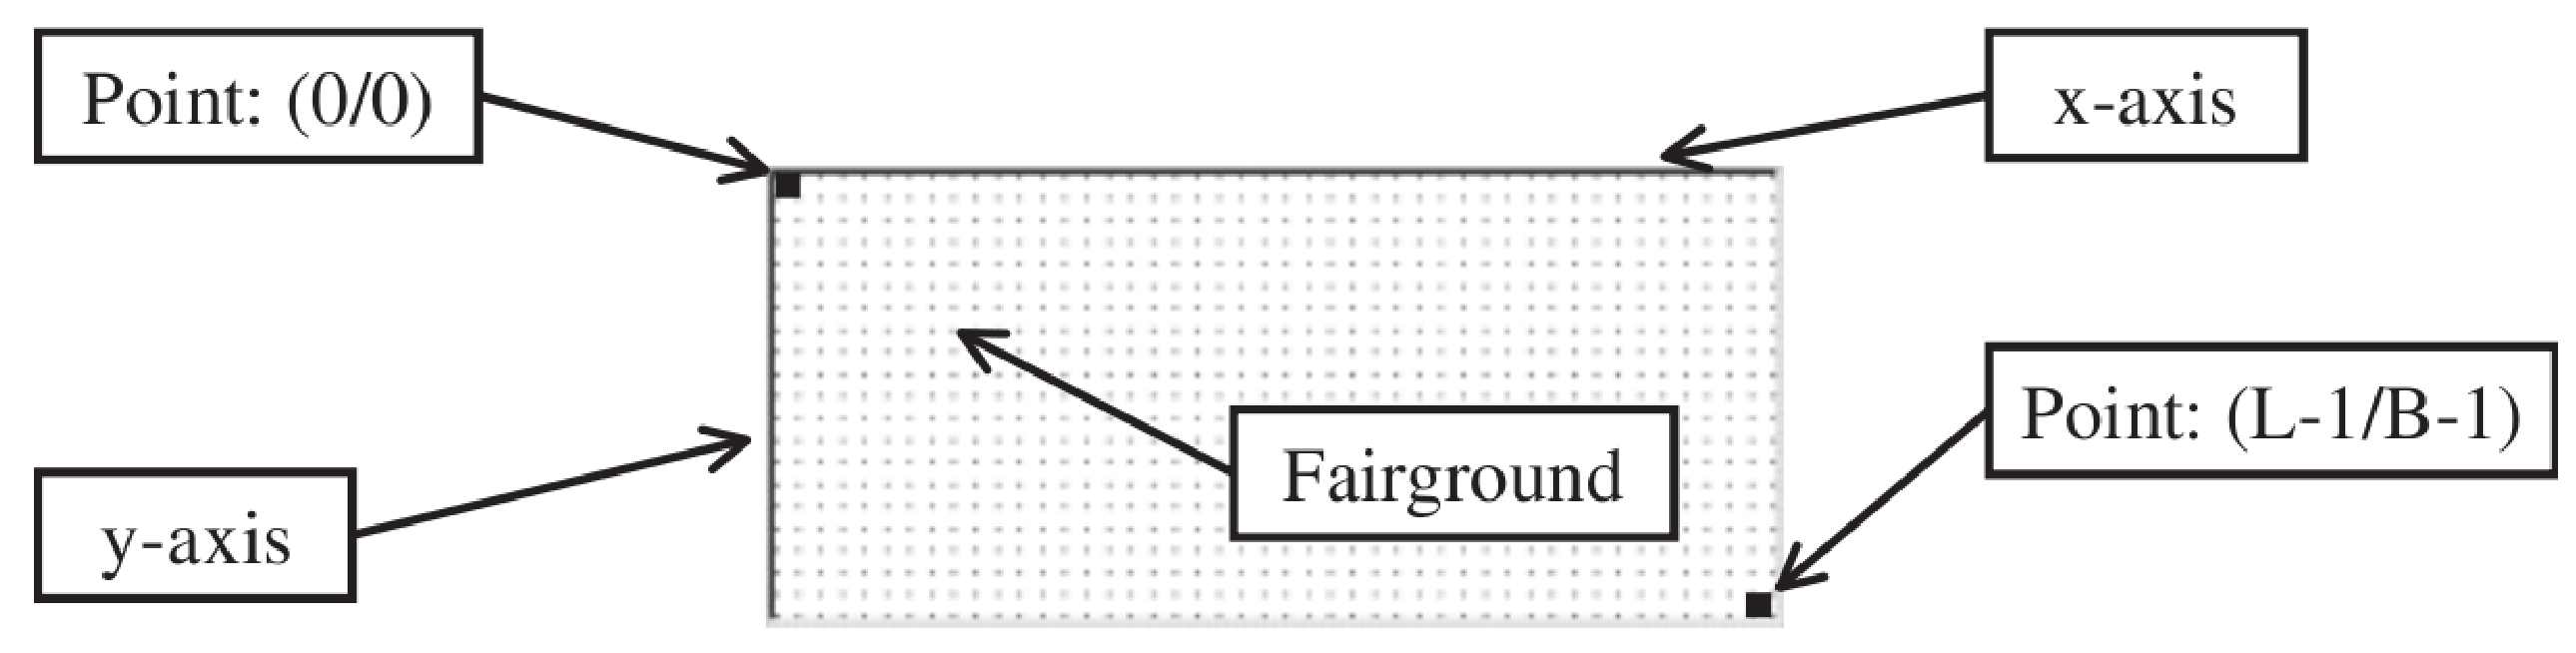
\includegraphics[width=10cm, height=3.5cm]{images/romont_fairground.eps}
\textit{\caption{\footnotesize fairground relativo allo spazio espositivo, associato ad un rettangolo su un piano cartesiano.}}
\end{figure} 
\\Per quanto riguarda gli stands, essi sono rappresentati come aree rettangolari o angolari (ad angolo) e le diverse tipologie di stand sono illustrate in figura 2.15; 
\begin{figure}[h]
\centering
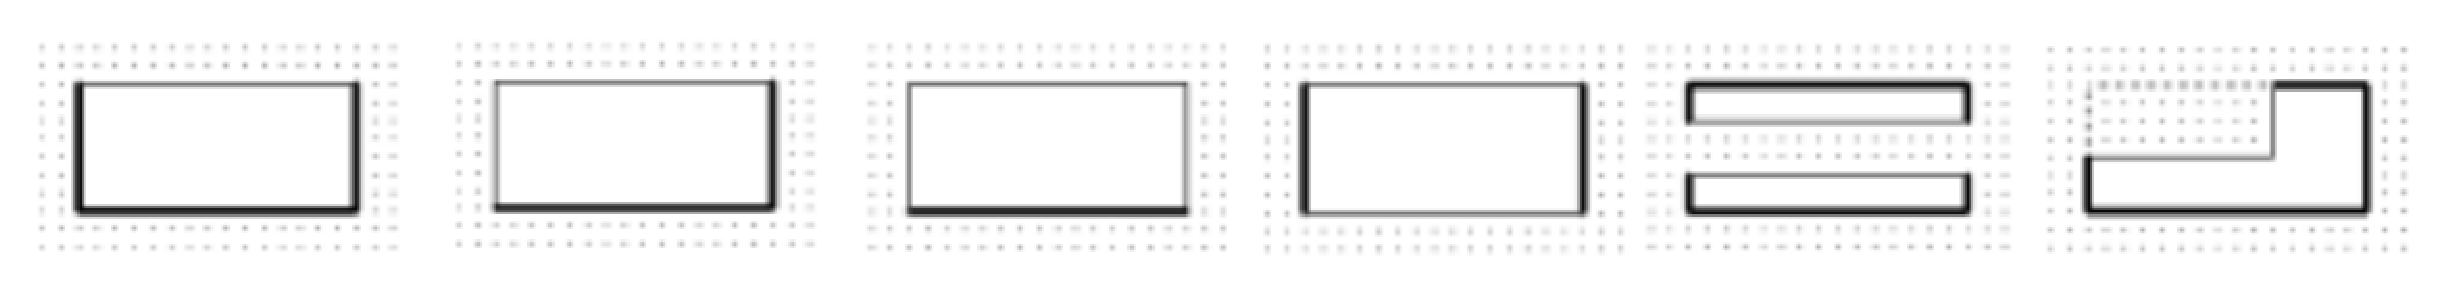
\includegraphics[width=12cm, height=2cm]{images/romont_stand_types.eps}
\textit{\caption{\footnotesize tipologie di stands/moduli impiegati nella fiera.}}
\end{figure} 
tali spazi espositivi possono essere posizionati verticalmente o orizzontalmente, a seconda delle esigenze, avendo perci\`{o} fino a 4 possibili orientamenti dello stand\footnote{supponiamo che le rotazioni possano avvenire ogni $90^{\circ}$}.
In figura 2.16 \`{e} possibile vedere come viene posizionato uno stand ad angolo all'interno della superficie, assieme ad una lista di valori che esprimono dimensioni e coordinate per il posizionamento.
\begin{figure}[h]
\centering
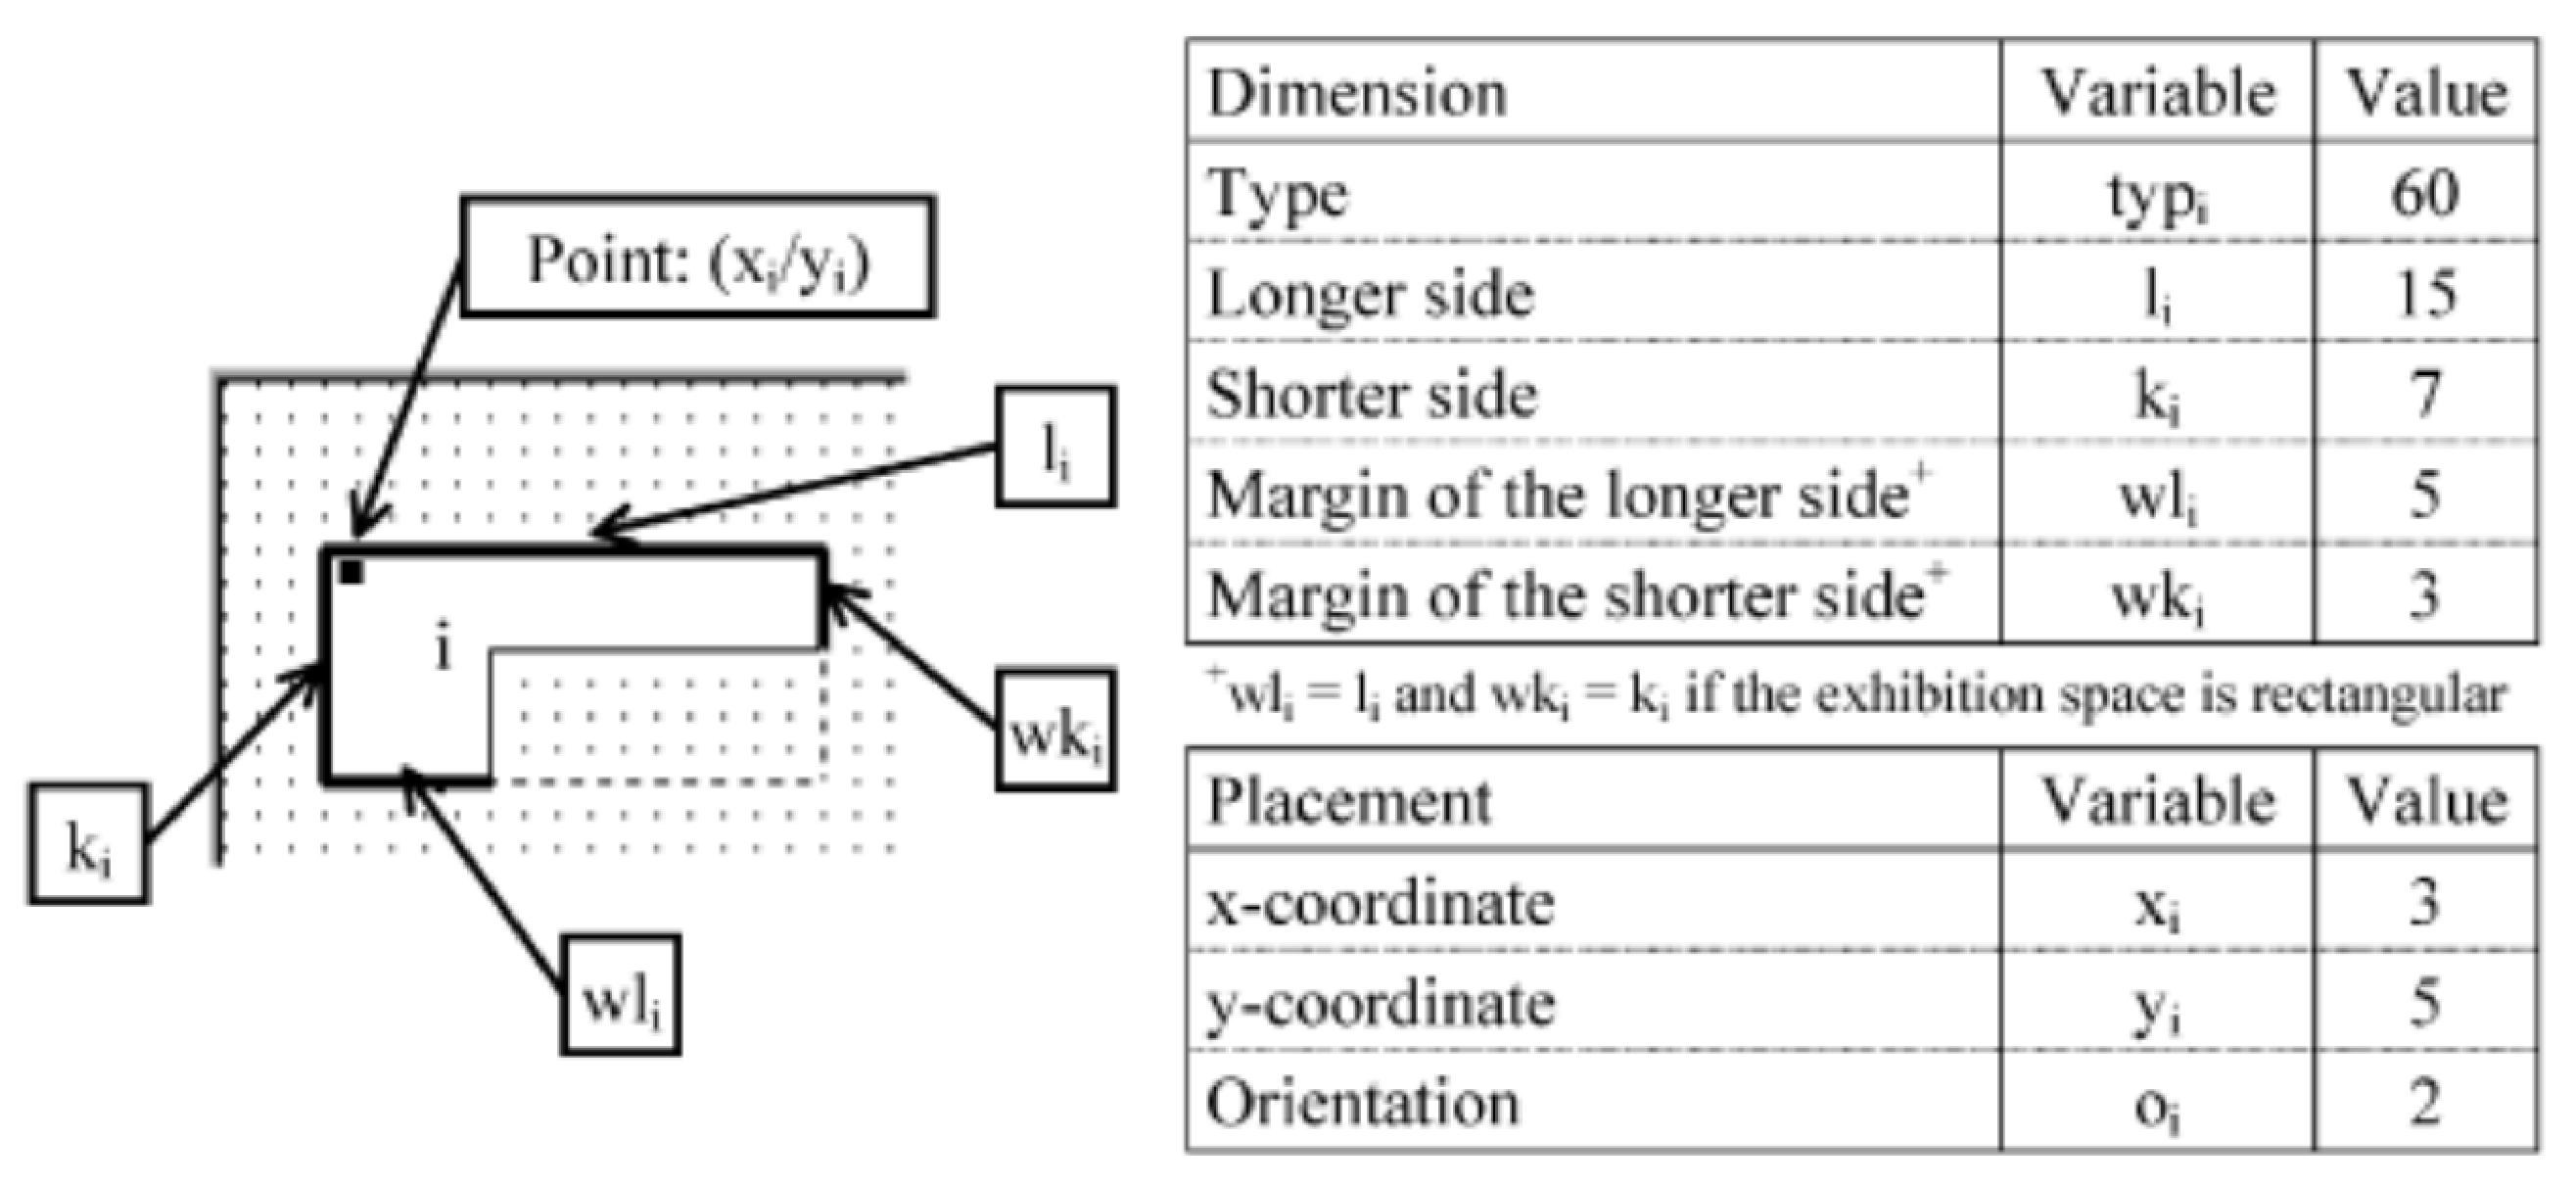
\includegraphics[width=12.5cm, height=5.5cm]{images/romont_placement.eps}
\textit{\caption{\footnotesize posizionamento di uno stand angolare $i$ sul fairground.}}
\end{figure} 
\\Si ha invece, per quanto concerne il percorso riservato ai visitatori, che il path non presenta alcun tratto curvilineo ed \`{e} quindi composto da tratti orizzontali e verticali (solo rettilinei) che devono essere paralleli agli assi cartesiani del rettangolo. Come si pu\`{o} vedere dalla figura 2.17, il quadrato nero indica un cambio di direzione del percorso, uno snodo che si pu\`{o} facilmente referenziare nell'algoritmo, perch\'{e} corrisponde esattamente ad una unit\`{a} base di misura.
\begin{figure}[h]
\centering
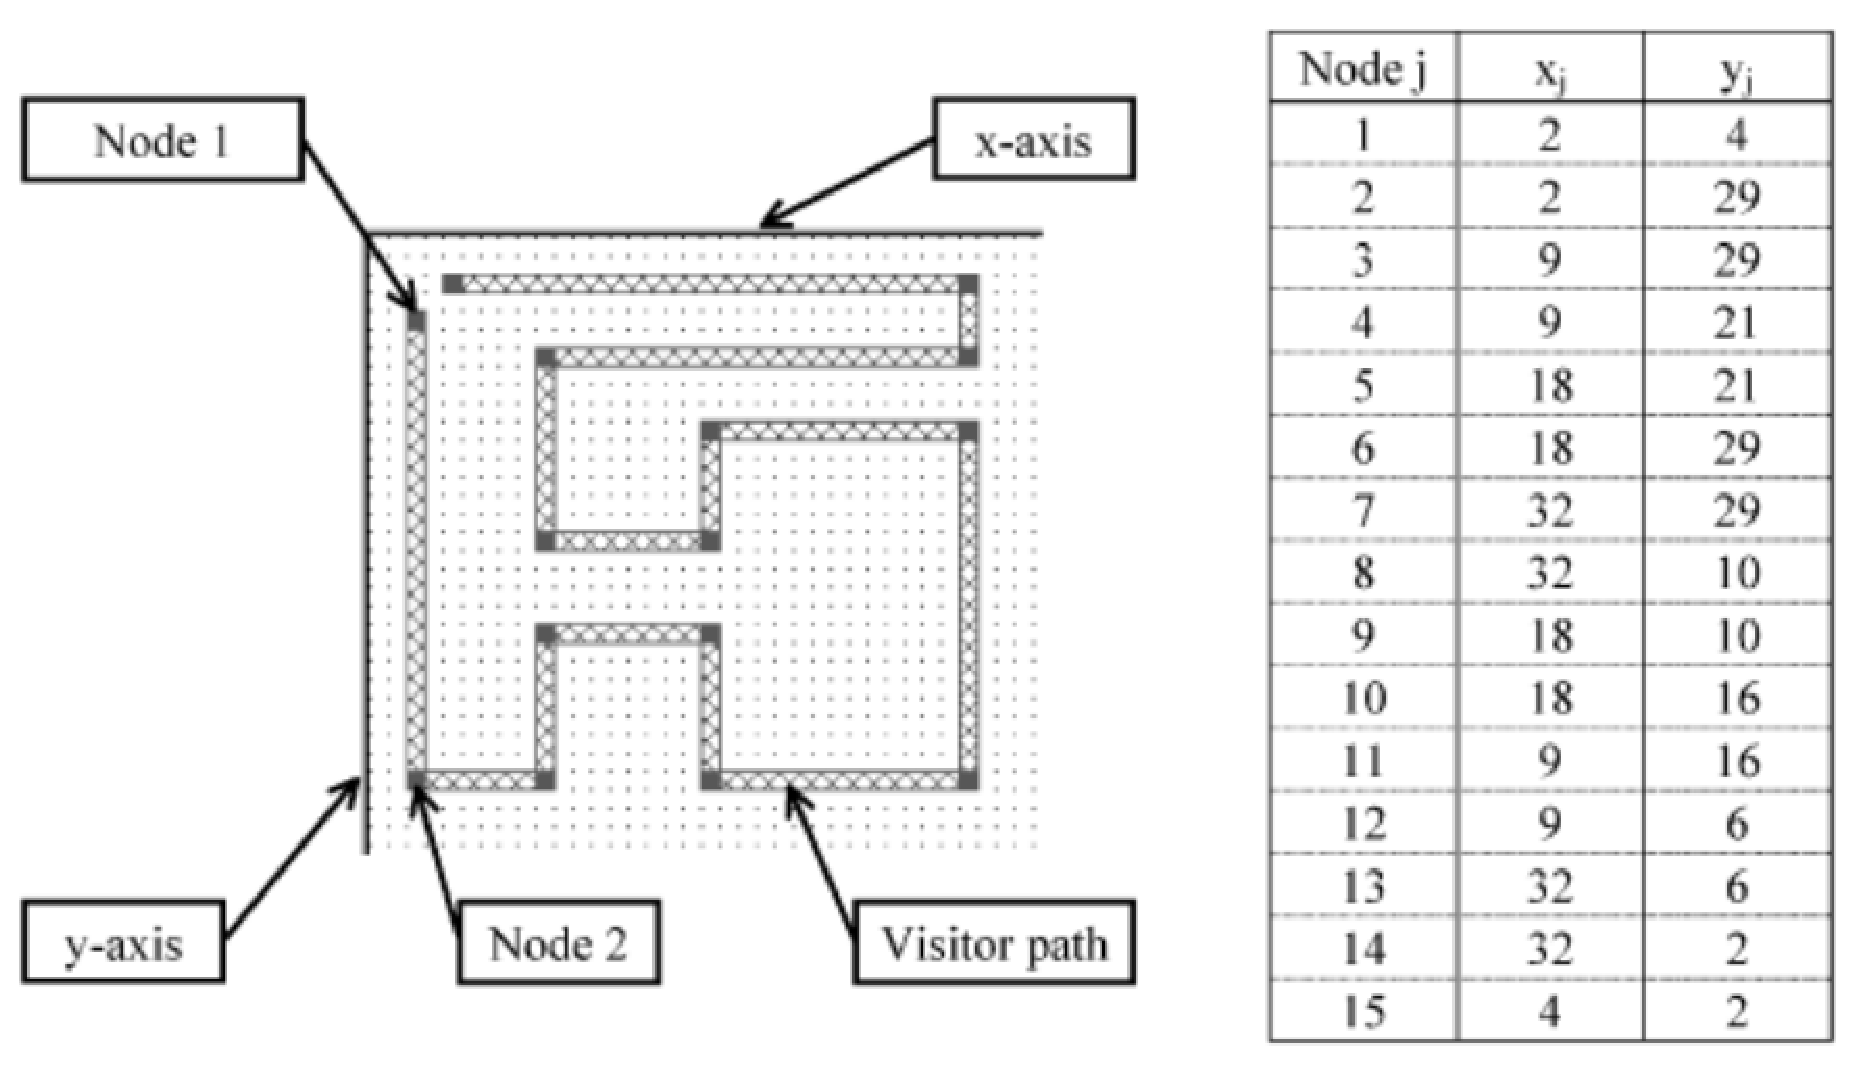
\includegraphics[width=10cm, height=5cm]{images/romont_path.eps}
\textit{\caption{\footnotesize percorso per i visitatori e relative coordinate.}}
\end{figure}    
\\L'\textit{adjacency model} implica la formulazione di tre criteri quantitativi per misurare la qualit\`{a} di un layout progettato bene; tali criteri derivano dai tre fattori visti in precedenza:
\begin{description}
\item[utilizzo degli spazi]: definiamo il coefficiente $r$ che esprime il rapporto tra la superficie rettangolare (il fairground) e la somma delle aree occupate dai padiglioni,
$$r = \dfrac{\sum_{i=1}^{N} ( (k_{i}\times l_{i}) - \left[(k_{i} - wk_{i}) \times (l_{i} - wl_{i})\right] )}{L \times B},$$ 
dove $N$ rappresenta il numero di stands, mentre $L$ e $B$ sono rispettivamente la lunghezza e la larghezza del fairground.\\ Notiamo che per padiglioni di forma rettangolare si ha $k_{i} = wk_{i}$ per cui il secondo addendo della sottrazione si annulla e quindi per questo caso la superficie viene calcolata solo tramite $k_{i} \times l_{i}$
\item[valore attrattivo]: tale requisito si misura grazie al calcolo dell'adiacenza $a_{i} = \frac{b_{i}}{q_{i}}$, dove il numeratore rappresenta la lunghezza del padiglione $i-esimo$ riferito al percorso della clientela e il denominatore indica la lunghezza dell'open space dello stand $i$-esimo. Due esempi autoesplicativi del calcolo delle adiacenze sono illustrati in figura 2.18. Indipendentemente dal fatto che la forma dell'item sia rettangolare o angolare, l'adiacenza viene calcolata considerando valori tra $0$ e $1$, che indicano la percentuale con cui la lunghezza dell'open side combacia col percorso. Se l'indice di adiacenza $a_{i}$ \`{e} alto, il valore attrattivo diventa importante, questo perch\'{e} si alzano le probabilit\`{a} che i visitatori si interessino al padiglione $i$-esimo
\item[agevolazioni ai visitatori]: questo fattore \`{e} piuttosto difficile da quantificare, perci\`{o} \`{e} stato adottato un criterio che consiste nel considerare due stands he si affacciano sullo stesso tratto di percorso. Introduciamo un coefficiente $f$ tale che
$$f = \dfrac{\sum_{i=1}^{N} b_{i}}{2 \times g},$$ dove $g$ indica la lunghezza del path dei visitatori.\\ Per varie ragioni il valore del coefficiente $f$ si preferisce che sia alto per quanto riguarda i visitatori
\end{description}
\begin{figure}[h]
\centering
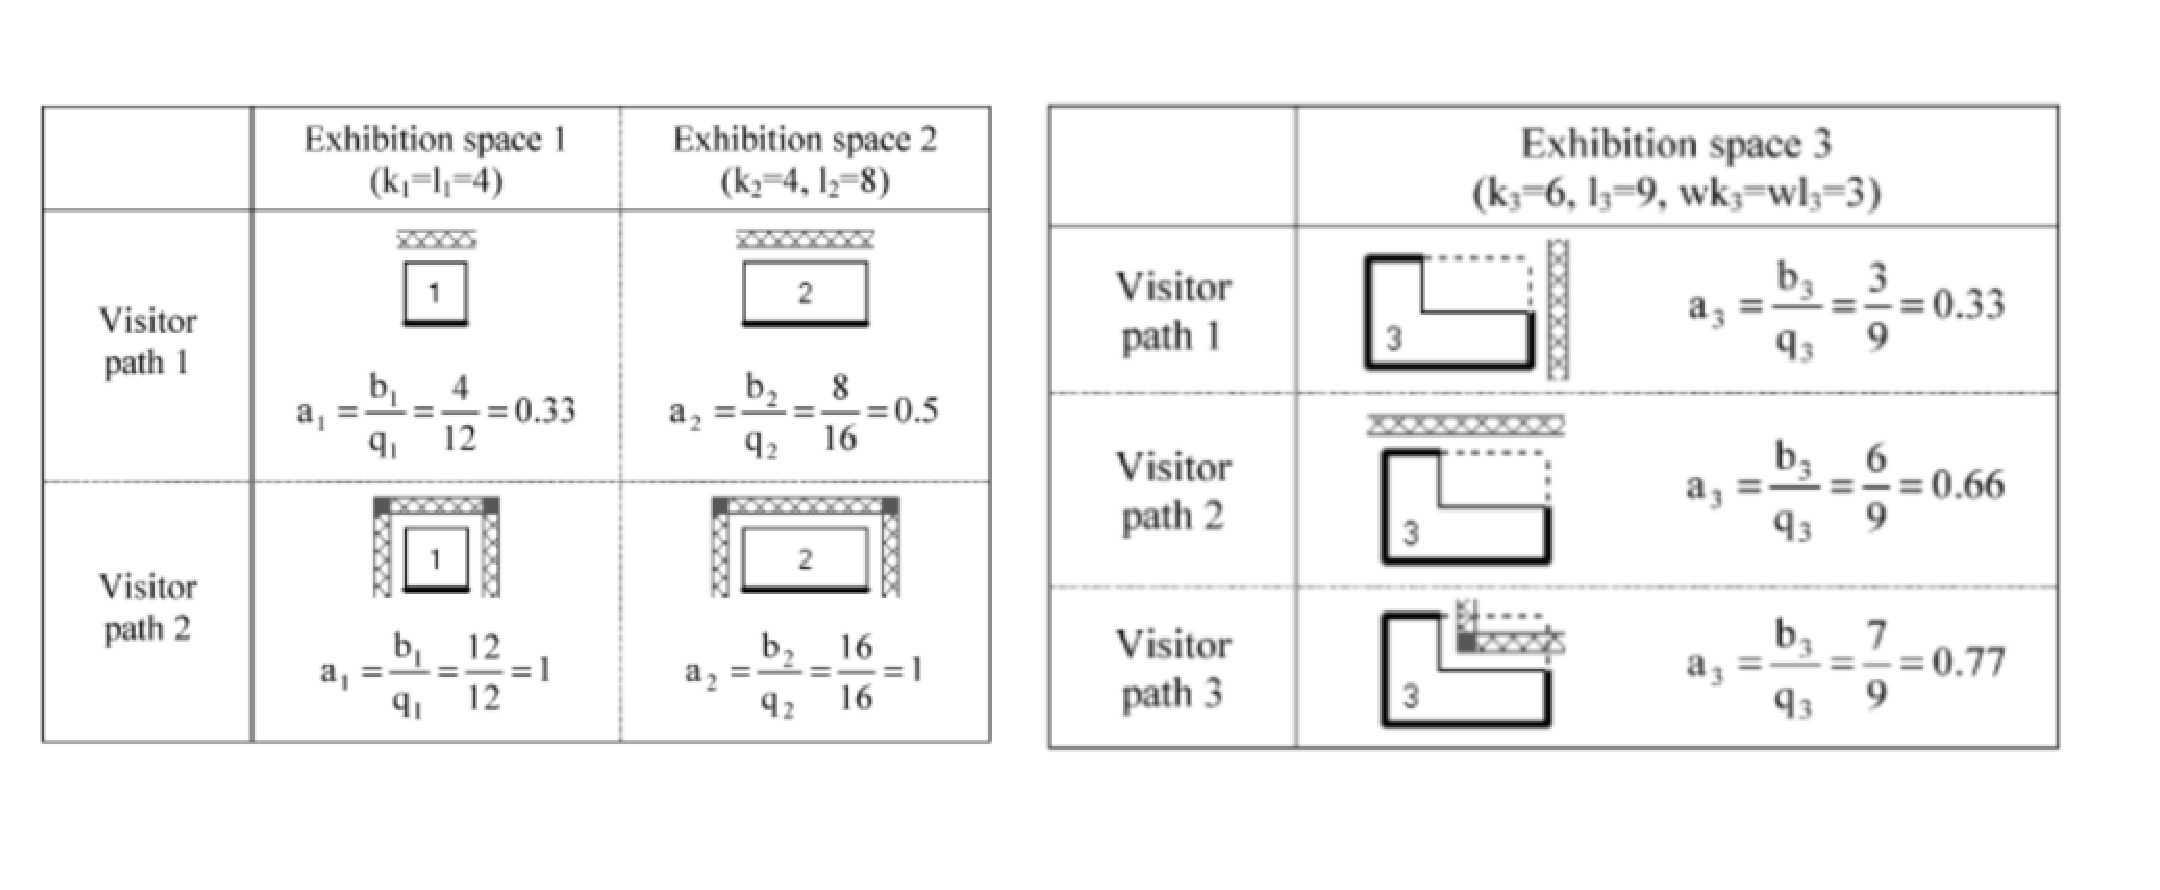
\includegraphics[width=14.5cm, height=6cm]{images/romont_adjacency.eps}
\textit{\caption{\footnotesize calcolo delle adiacenze: nel primo caso sono calcolate quattro combinazioni in base all'entit\`{a} degli stand e del path, mentre nel secondo ne sono calcolate tre, con un solo tipo di stand ma con tre tipologie di percorso.}}
\end{figure} 
Applicando queste soluzioni ad un caso reale (l'edizione della fiera del 2000) si sono riscontrati risultati soddisfacenti e il layout ottenuto \`{e} stato calcolato in base a questi tre criteri di progetto. In particolare si evidenziano i fattori $f = 80\%$ e $\bar{a}_{i} = 84\%$ dove quest'ultimo rappresenta l'indice di adiacenza medio riscontrato. Come \`{e} illustrato in figura 2.19, gli stands pi\`{u} chiari (la maggioranza) corrispondono ad un \textit{adjacency index} tra $0$ e $0.5$, mentre le zone pi\`{u} scure vanno da $0.5$ a $1$.\\
\begin{figure}[h]
\centering
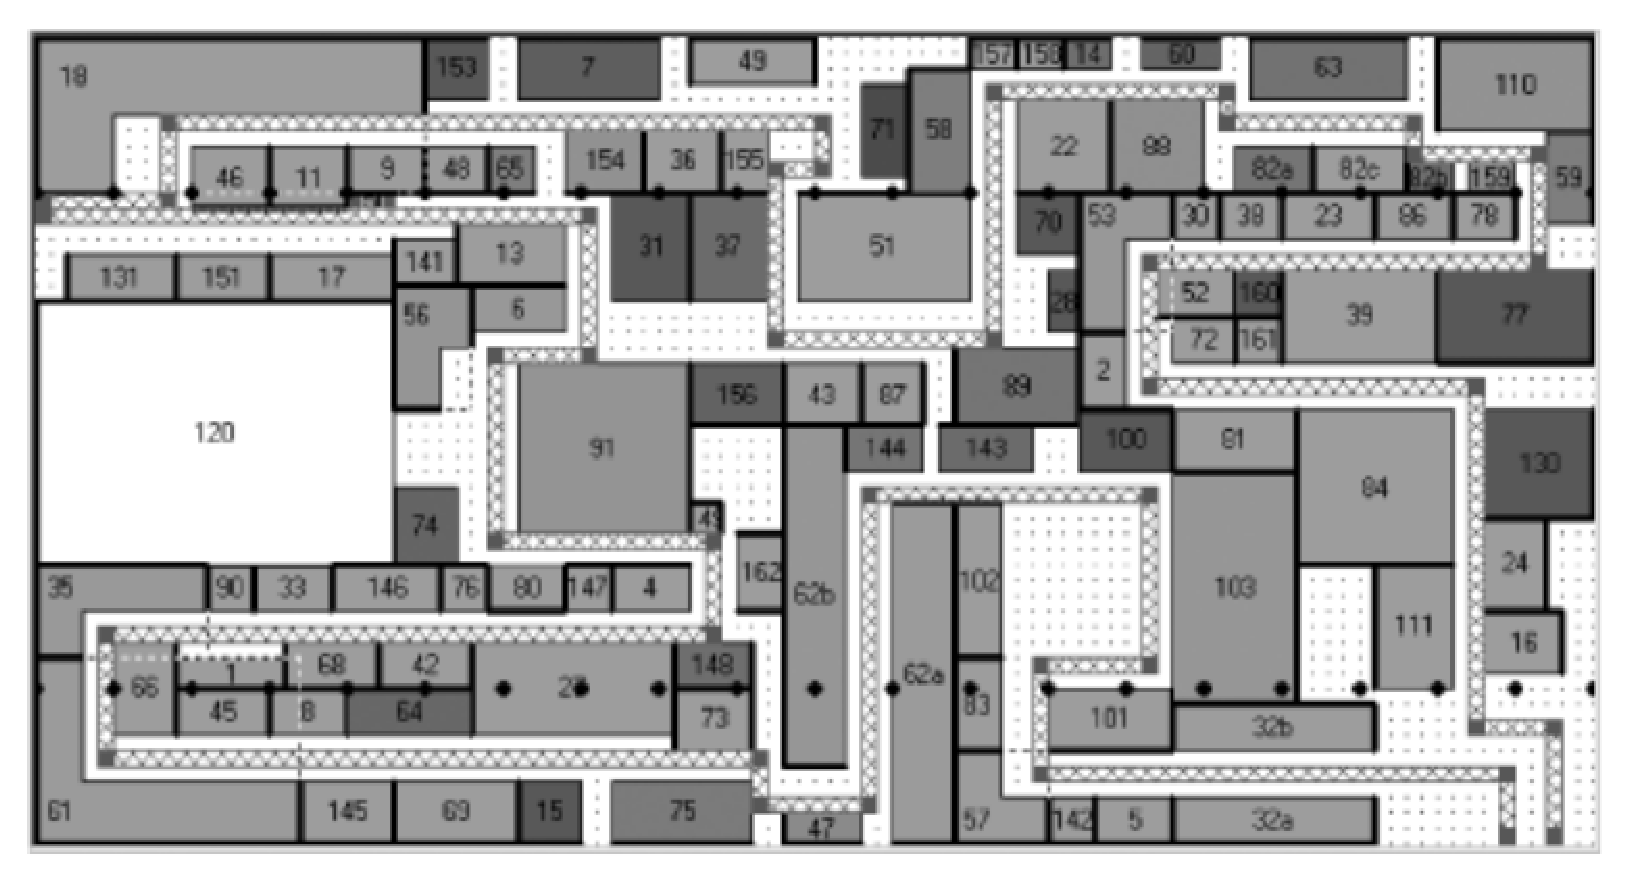
\includegraphics[width=12cm, height=5.5cm]{images/romont_fairgr_adj.eps}
\textit{\caption{\footnotesize risultato finale dell'adjacency model applicato all'esposizione del 2000.}}
\end{figure}
\\Basandosi perci\`{o} sull'adjacency model possiamo costruire un modello di layout partendo da una configurazione iniziale che consiste nel posizionare uno spazio di seguito all'altro accanto al percorso prestabilito per i visitatori, dove quest'ultimo viene gi\`{a} fornito all'inizio assieme ad alcuni stand che sono gi\`{a} disposti per motivi molteplici.
A questo proposito sono stati sviluppati tre algoritmi per procedere al piazzamento degli spazi espositivi della fiera di Romont.\\ I dati di input degli algoritmi sono costituiti da dati concernenti le dimensioni degli stands e il layout iniziale. In particolare intendiamo per layout iniziale la configurazione che include le dimensioni $L \times B$ del fairground, le coordinate $(x_{i}, y_{i})$ dei nodi del percorso e i dati sul posizionamento degli stand rettangolari e angolari $(o_{i}, x_{i}, y_{i})$.\\
In figura 2.20 \`{e} raffigurato un layout iniziale della fiera di Romont, in cui sono dati il path e gli stand pre-posizionati e in cui vanno installati tutti i rimanenti spazi espositivi, raggruppati nella parte sinistra dell'immagine. Come dati iniziali vengono quindi forniti $g = 508$ e $M = 35$, ovvero la lunghezza del path in unit\`{a} di area e il numero di nodi, rispettivamente. L'algoritmo non fa altro che scegliere gli items rettangolari, coerentemente coi criteri adottati, e piazzarli nel fairground finch\`{e} non si raggiunge un layout finale. L'output dell'algoritmo sar\`{a} costitutito perci\`{o} dai dati relativi agli stands posizionati, quindi $(o_{i}, x_{i}, y_{i})$, e dal numero di stands che non \`{e} stato possibile includere. \\
\begin{figure}[h]
\centering
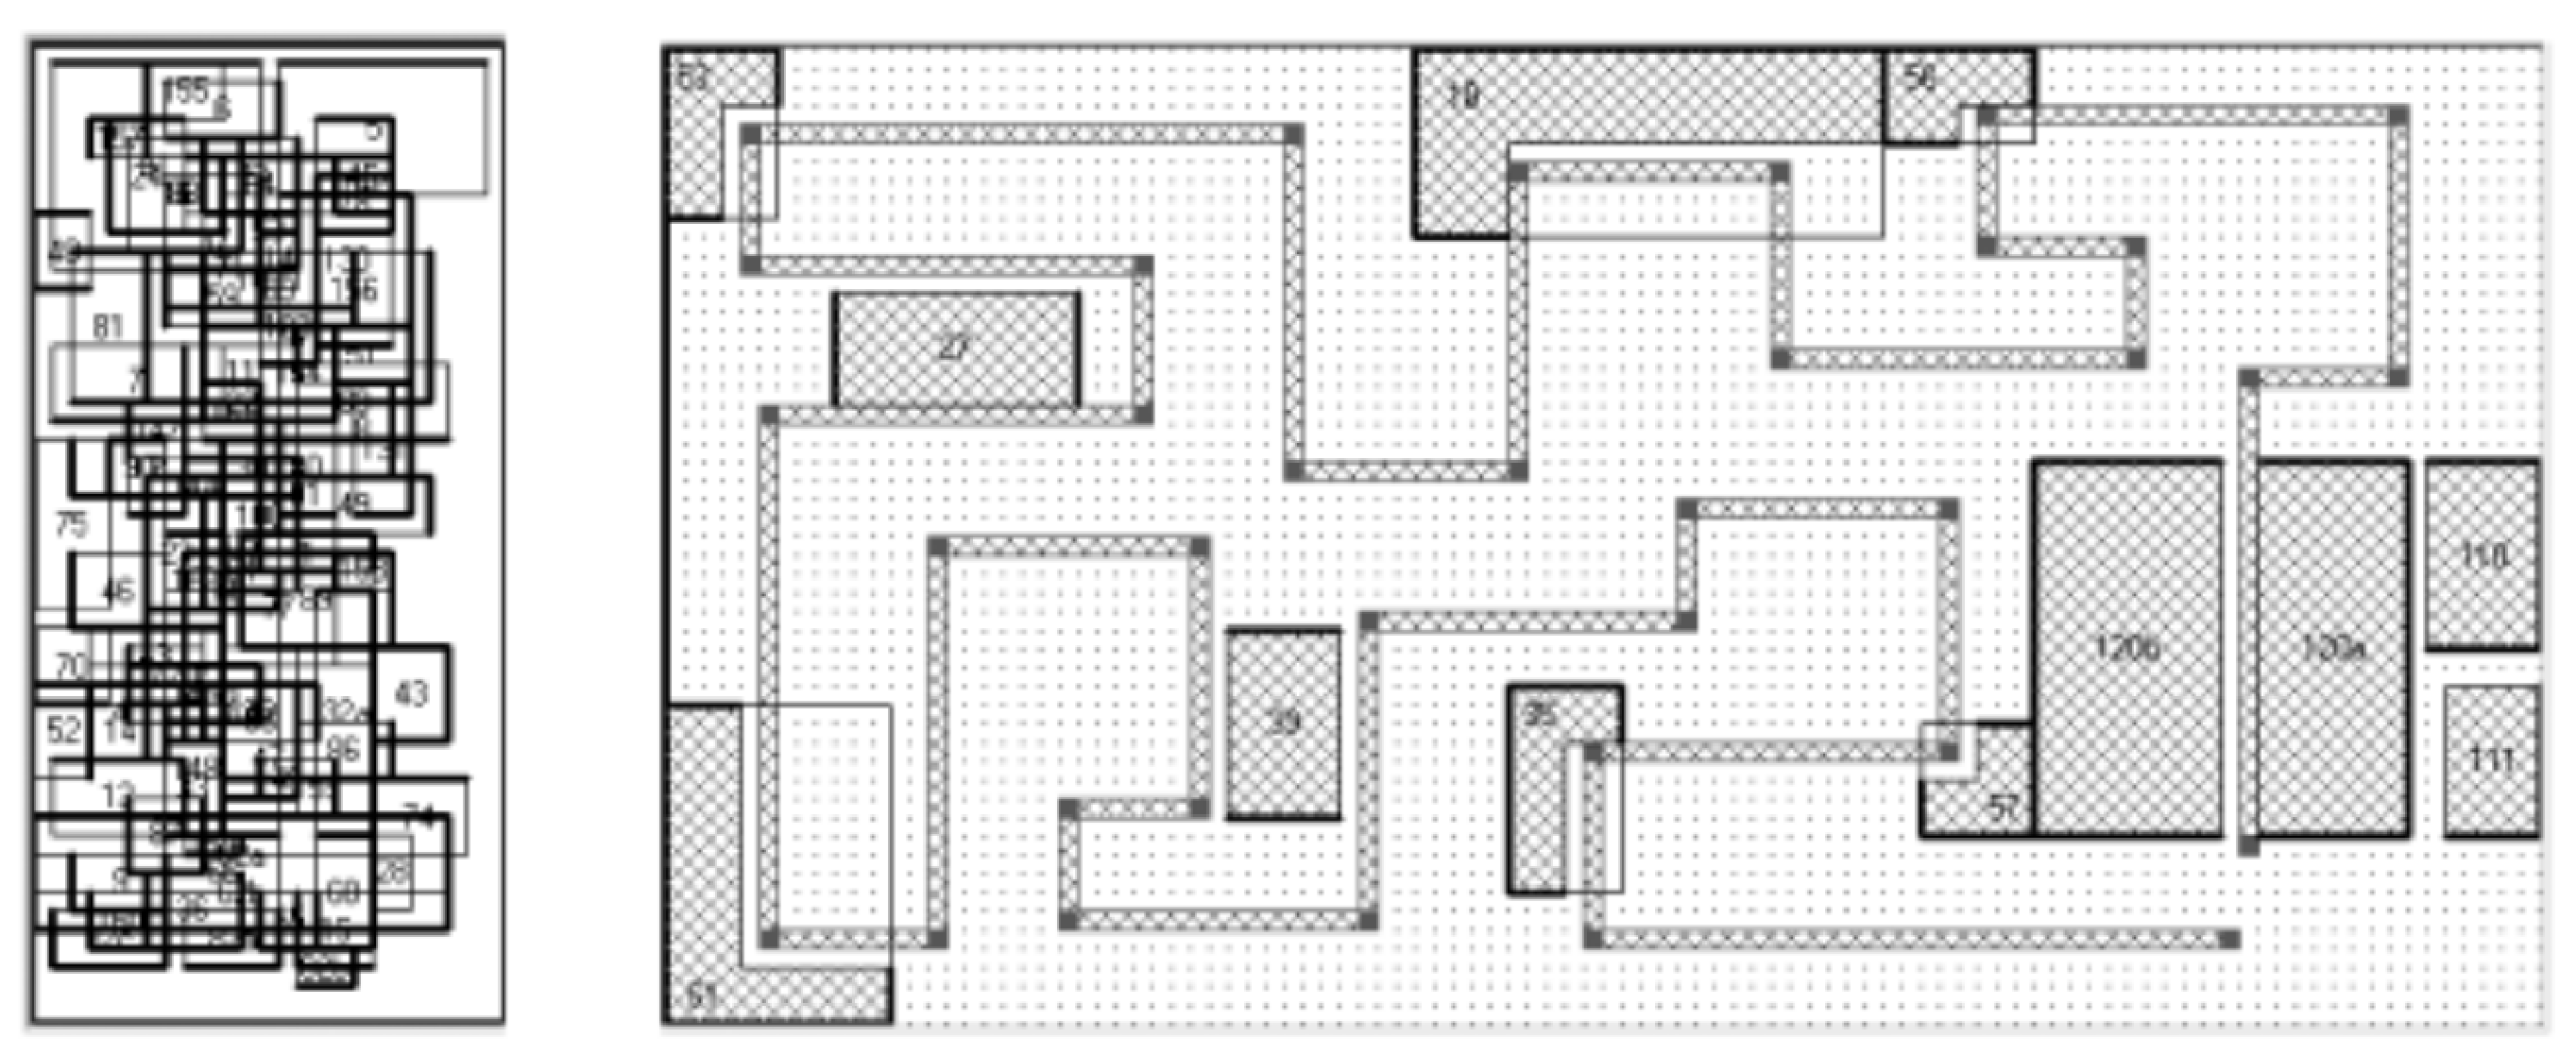
\includegraphics[width=12cm, height=5.5cm]{images/romont_start.eps}
\textit{\caption{\footnotesize layout di partenza della fiera di Romont dove si vedono il path e alcuni stand preposizionati, mentre a sinistra sono raggruppati gli altri stand da includere nel progetto.}}
\end{figure}
\\Diamo adesso alcune definizioni che ci permettono di proseguire con l'analisi:
\begin{itemize}
\item definiamo \textit{path section} una porzione di percorso delimitata da due nodi e quindi in maniera pi\`{u} semplice un segmento di percorso; se consideriamo segmenti orizzontali si hanno due direzioni che sono est e ovest, mentre per quelli verticali si parler\`{a} di nord e sud; un cambio di direzione del percorso si ha quando si \`{e} all'inizio o alla fine di ciascun segmento, e in questo caso si pu\`{o} girare a destra ($d_{j}=R$) o a sinistra ($d_{j}=L$)
\item definiamo \textit{corridoi laterali} quegli spazi, ortogonali al percorso, necessari a garantire che uno stand sia accessibile attraverso entrate alternative, che non si affacciano necessariamente al path
\item i \textit{candidate points} sono le coordinate di ogni vertice di uno stand che pu\`{o} essere piazzato interamente nel layout grazie al fatto che tutte le coordinate soninterne all'area selezionata per il posizionamento. Inoltre sono \textit{candidate points} anche quei punti in cui un nodo del percorso non influisce sullo stand, ad esempio andando a tagliare internamente lo stand
\end{itemize} 
A questo punto proseguiamo con l'illustrare il primo algoritmo, il quale ha come scopo quello di testare la possibilit\`{a} di piazzamento di uno spazio nel fairground, definendo tra i vari \textit{constraints} anche la larghezza minima dei corridoi laterali e l'adiacenza dello stand al percorso. In particolare l'algoritmo determina se uno stand \`{e} idoneo o meno ad entrare nel rettangolo riservato all'esposizione: in caso positivo significa che lo stand non si sovrappone a nessun altro stand gi\`{a} presente, che non invade lo spazio riservato al path o ad altri elementi, che risiede interamente all'interno del rettangolo e che, infine, fornisce una larghezza minima del corridoio laterale idonea a quanto previsto.\\ Utilizzando per\`{o} questa soluzione si ottiene un layout che esclude alcuni spazi espositivi e dunque \`{e} necessaria una riformulazione dell'algoritmo che consideri non pi\`{u} una ottimizzazione riferita ad un solo lato del segmento del path adiacente allo stand, bens\`{i} tutti i lati a contatto con esso. Tale aggiornamento sar\`{a} identificato come secondo algoritmo: questo approccio rivela che alcune aree del percorso dei visitatori non sono usate appieno e che le aree disponibili che si incontrano all'inizio del percorso sono pi\`{u} occupate rispetto a quelle che si trovano verso la fine. Questo accade perch\'{e} l'algoritmo2 valuta le posizioni partendo proprio dal nodo iniziale del path.\\ Un'ulteriore tecnica per "`"`raffinare"'"' la procedura consiste nel distribuire in maniera pi\`{u} uniforme gli stands lungo il percorso usufuendo al massimo degli spazi inutilizzati. L'algoritmo3 combina perci\`{o} le qualit\`{a} positive delle due versioni precedenti e rappresenta una versione definitiva e ultimata del layout, perch\'{e} permette di realizzare un progetto ottimo che soddisfa i requisiti e le specifiche e che riesce ad includere tutti gli stands nel fairground.
In figura 2.21 sono rappresentate le tre versioni dell'algoritmo usato nell'edizione della fiera di Romont del 2000; si riconduce a fine capitolo per quanto riguarda la formuazione degli algoritmi secondo uno pseudo-linguaggio.\\
\begin{figure}[h]
\centering
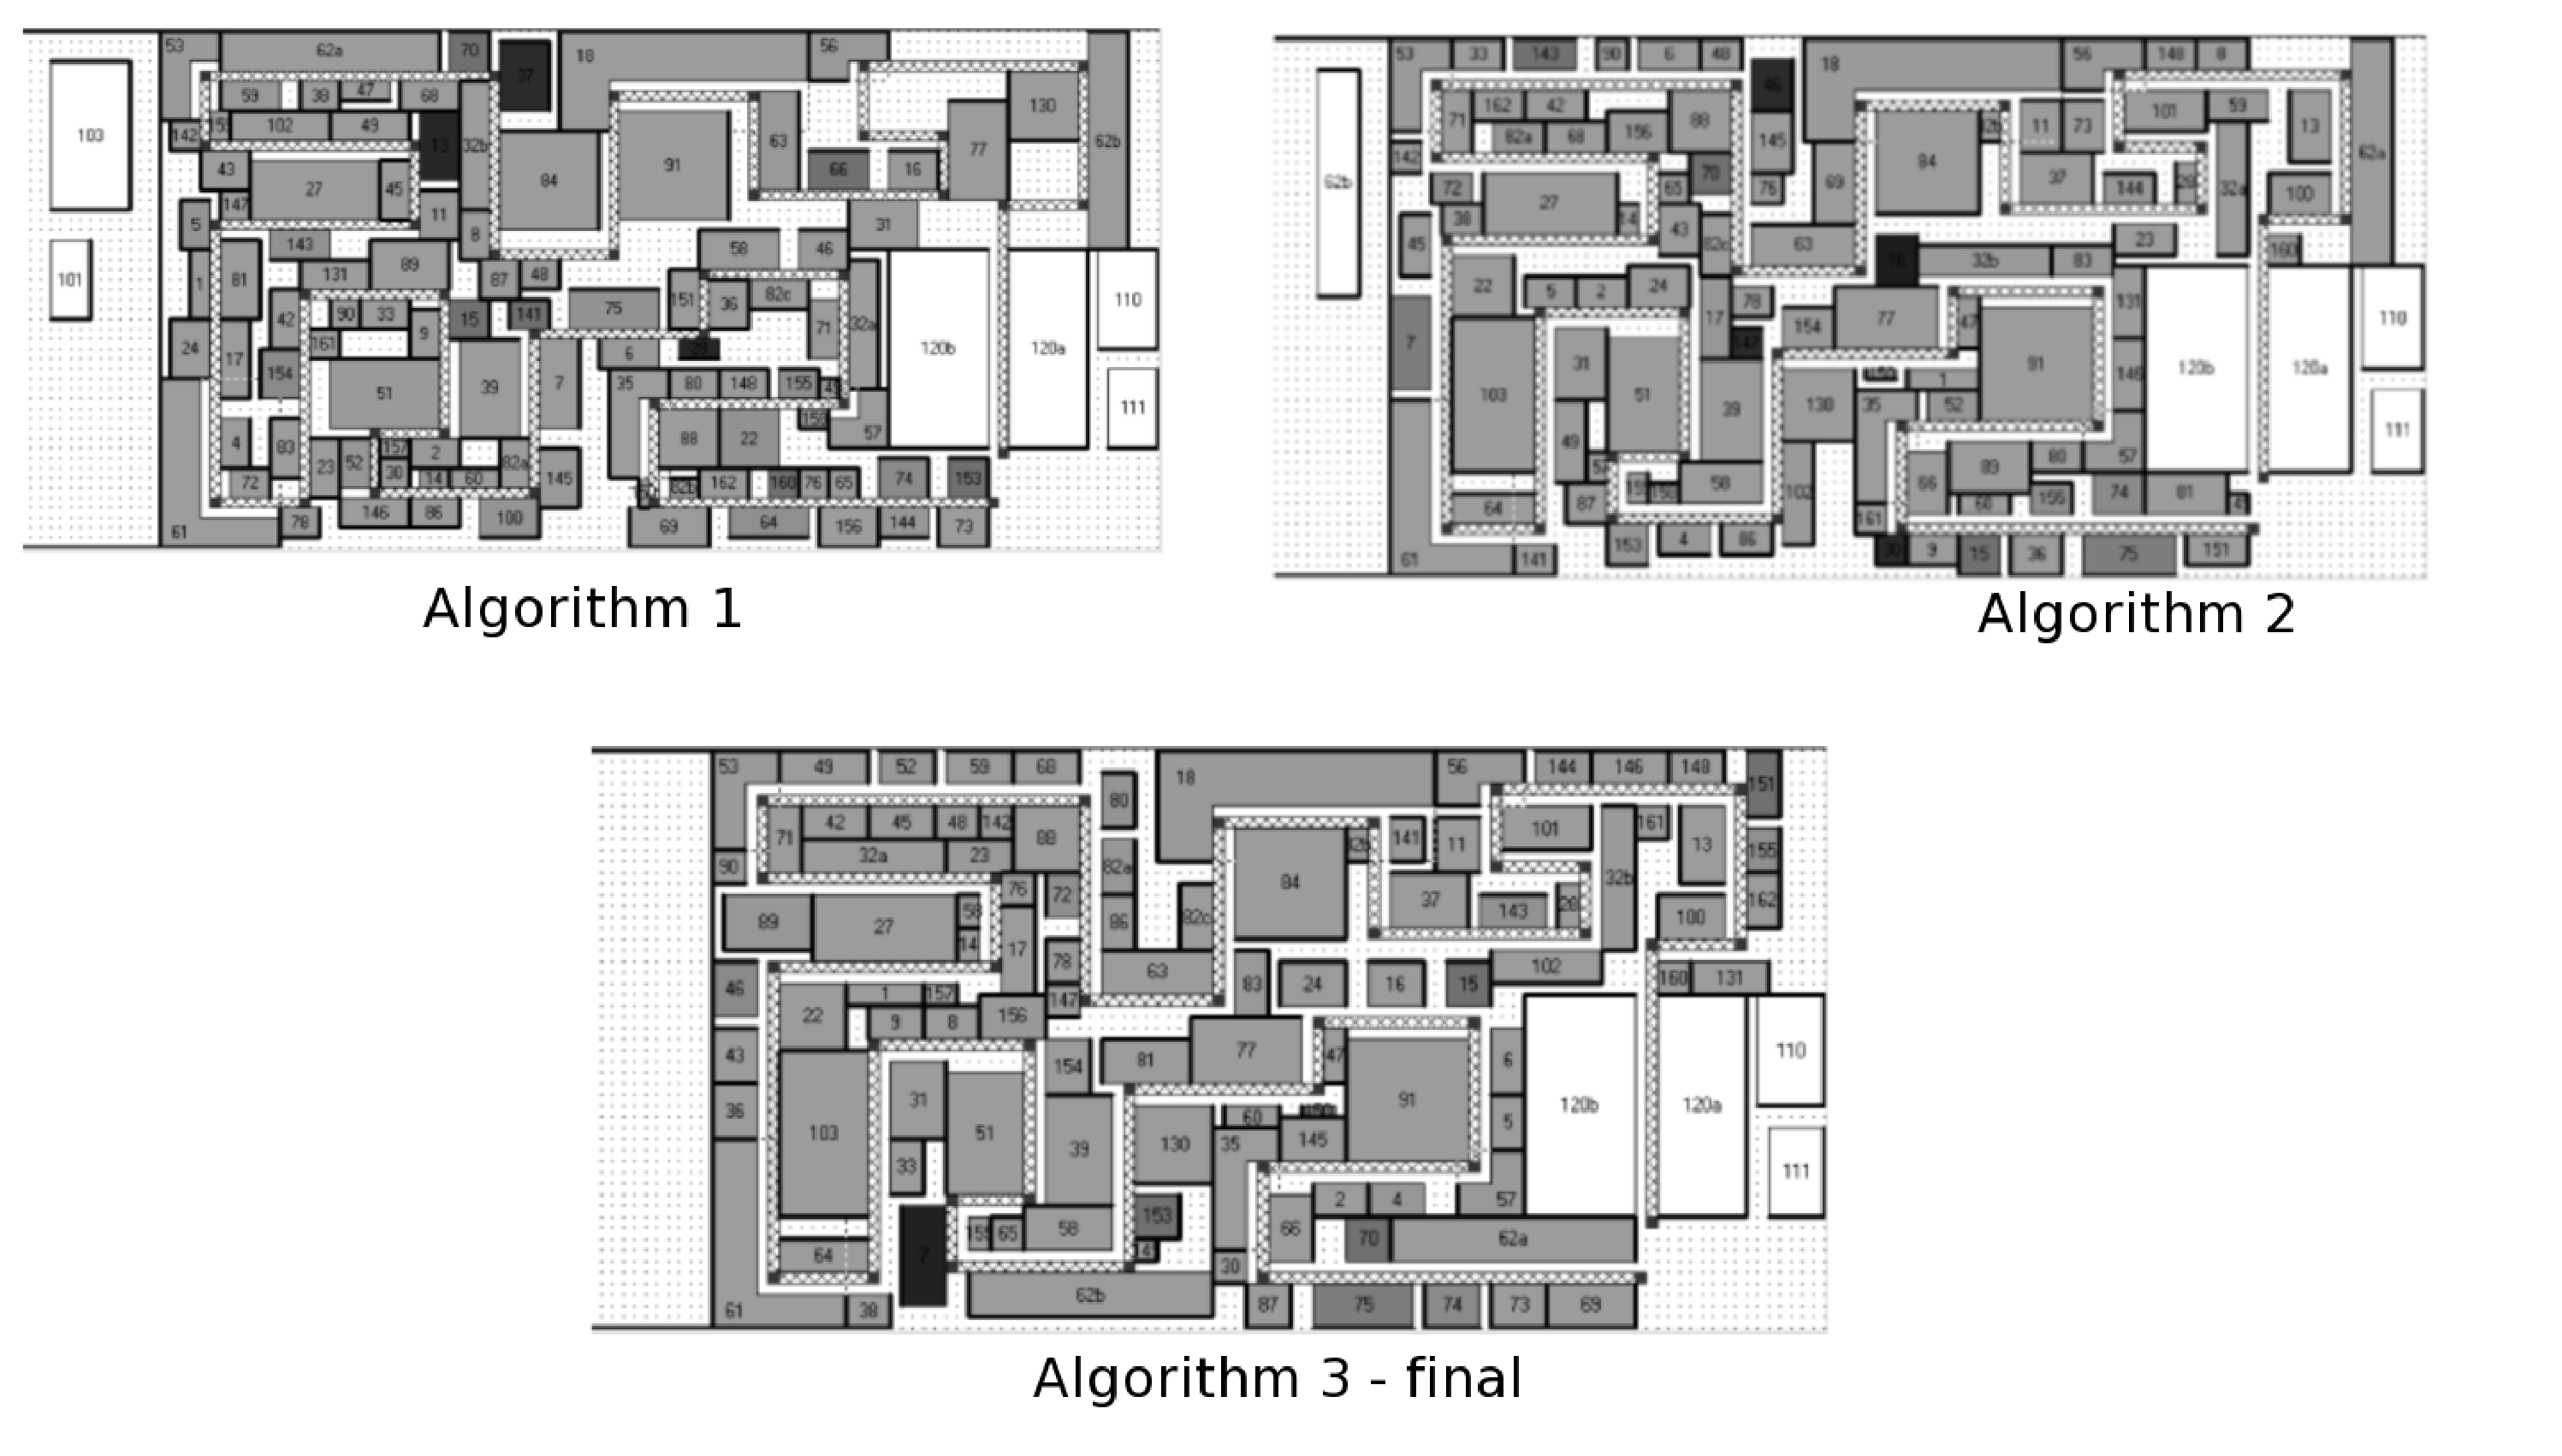
\includegraphics[width=14.5cm, height=7.5cm]{images/romont_3_algorithms.eps}
\textit{\caption{\footnotesize tre versioni dell'algoritmo impiegato per il layout ottimo dell'esposizione del 2000.}}
\end{figure}
\\I risultati ottenuti applicando l'algoritmo nella sua versione finale mostrano che la procedura di costruzione genera risultati promettenti, basandosi sul modello dell'adiacenza. Inoltre i tre criteri precedentemente analizzati (utilizzo degli spazi, valore attrattivo e agevolazioni ai clienti visitatori) sono confinati in intervalli di accettabilit\`{a} e i valori dei coefficienti $f$ sono pi\`{u} alti di quelli riscontrati usando un layout "`"`manuale"'"'. Il coefficiente $r = 0.64$ che misura il buono sfruttamento dello spazio \`{e} il migliore riscontrato.\\
Tutti i calcoli e le elaborazioni sono stati effettuati su una macchina con processore Pentium a 200MHz con gli algoritmi implementati mediante il linguaggio Visual Basic 6.0, per un tempo impiegato dal calcolatore che va da un minimo di $9.78$ e $15.42$ secondi. L'algoritmo 3 impiega normalmente un secondo in pi\`{u} rispetto all'algoritmo 2, che prevede minor complessit\`{a}.\\ 

\subsection{Considerazioni finali}
La disposizione degli stand in ambito fieristico non \`{e} ancora particolarmente soggetta a studi scientifici, tuttavia lo studio precedentemente eseguito ha qualche parallelismo con il calcolo del layout aziendale; di solito un layout fieristico tiene conto di pi\`{u} criteri, invece in un layout aziendale il criterio fondamentale \`{e} quello di minimizzare i costi. Per quanto riguarda la fiera di Romont si sono utilizzati diversi criteri per avvicinarsi ad una soluzione accettabile.
La procedura su cui si basavano i tre algoritmi visti precedentemente era improntata sulla collocazione degli stand dato un certo percorso prefissato e dati dei layout iniziali; proprio questi ultimi tendono ad influenzare maggiormente il raggiungimento di un possibile layout finale, il quale dipende da:
\begin{multicols}{2}
\begin{itemize}
\item dimensioni della superficie espositiva
\item lunghezza del percorso (path)
\item numero di cambi di direzione nel percorso (nodi)
\item posizione (in coordinate cartesiane) degli angoli degli percorso
\item posizione obbligatoria e irremovibile di alcuni stands
\end{itemize}
\end{multicols}
Negli algoritmi precedentemente studiati gli stand venivano collocati uno alla volta; si potrebbe invece velocizzare il procedimento usando un algoritmo di packing in grado di collocare diversi stand nello stesso momento. La creazione del percorso iniziale pu\`{o} essere considerata come un importante problema anche se \`{e} solo l'inizializzazione del layout; l'individuazione di un percorso ideale faciliterebbe il raggiungimento di una soluzione accettabile finale. \\
\\Per ci\`{o} che riguarda la fiera di Fortaleza, invece, si pu\`{o} concludere affermando che l'implementazione dei due tipi di FLOP ci ha portati all'ottenimento del nostro traguardo, potendo appunto affermare che il numero di stand che si possono collocare all'interno dell'area espositiva di Fortaleza \`{e} maggiore di quello del layout precedente.\\
\\
\begin{figure}[h]
\centering
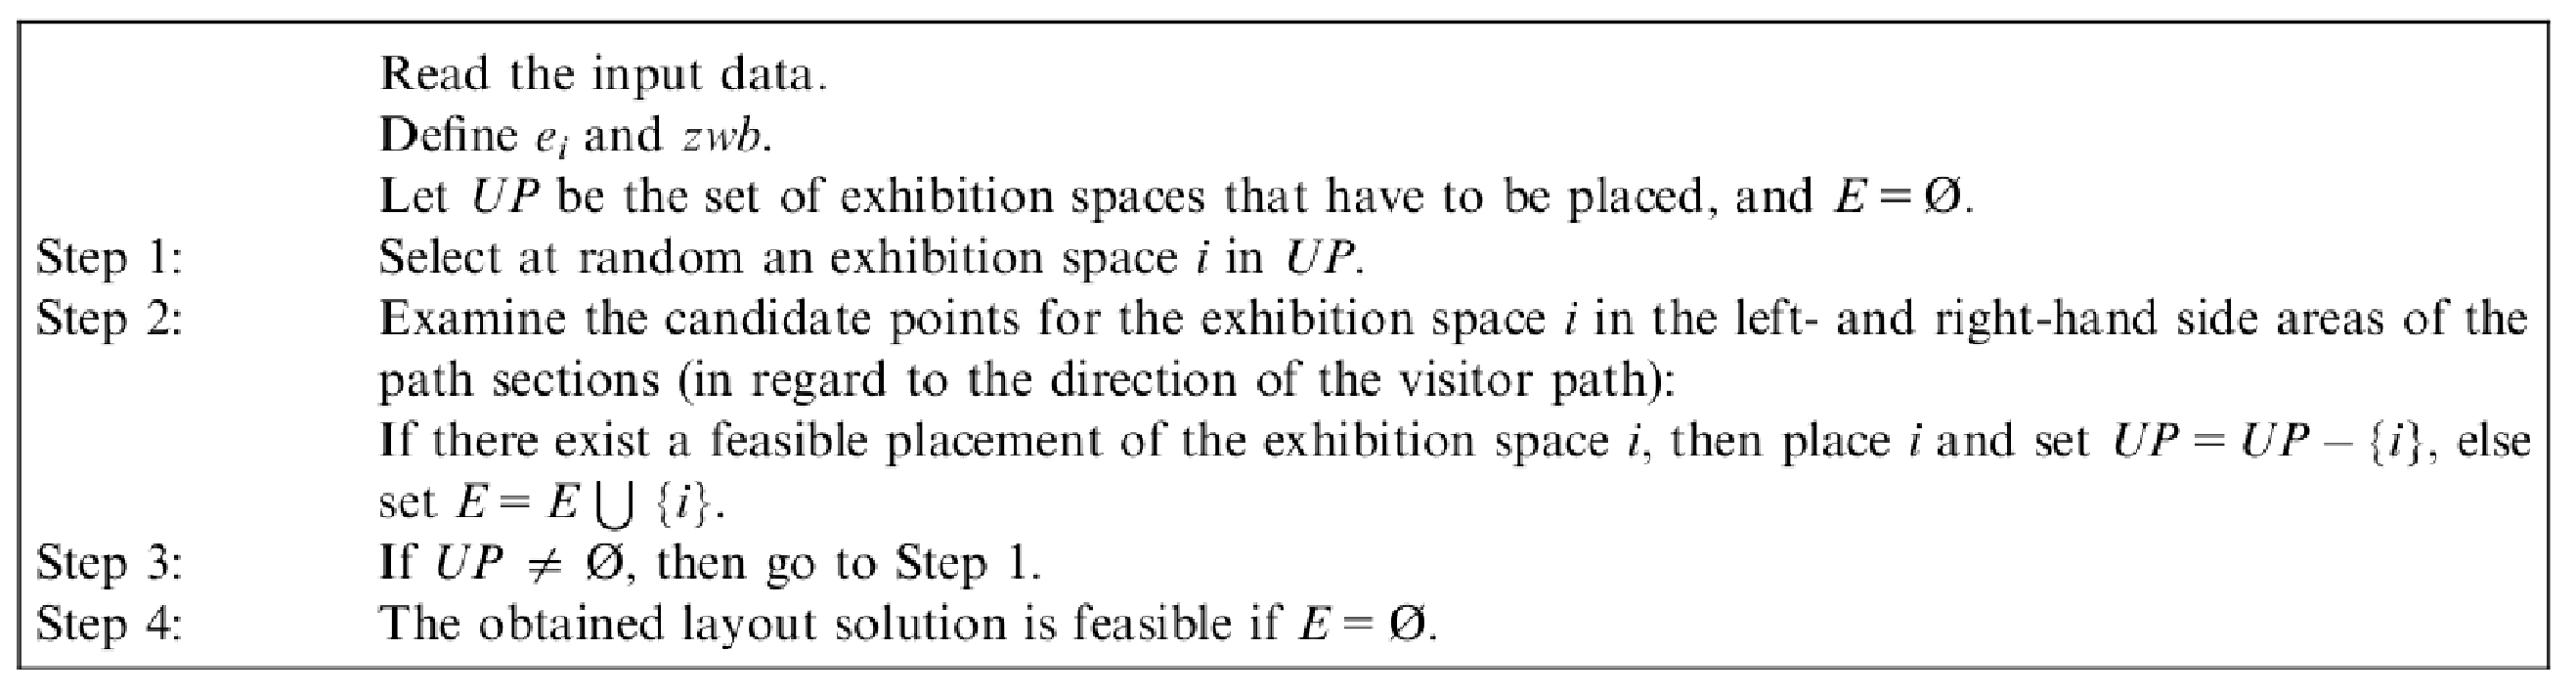
\includegraphics[width=15cm, height=4.5cm]{images/algo1.eps}
\textit{\caption{\footnotesize Algoritmo 1.}}
\end{figure}
\begin{figure}[h]
\centering
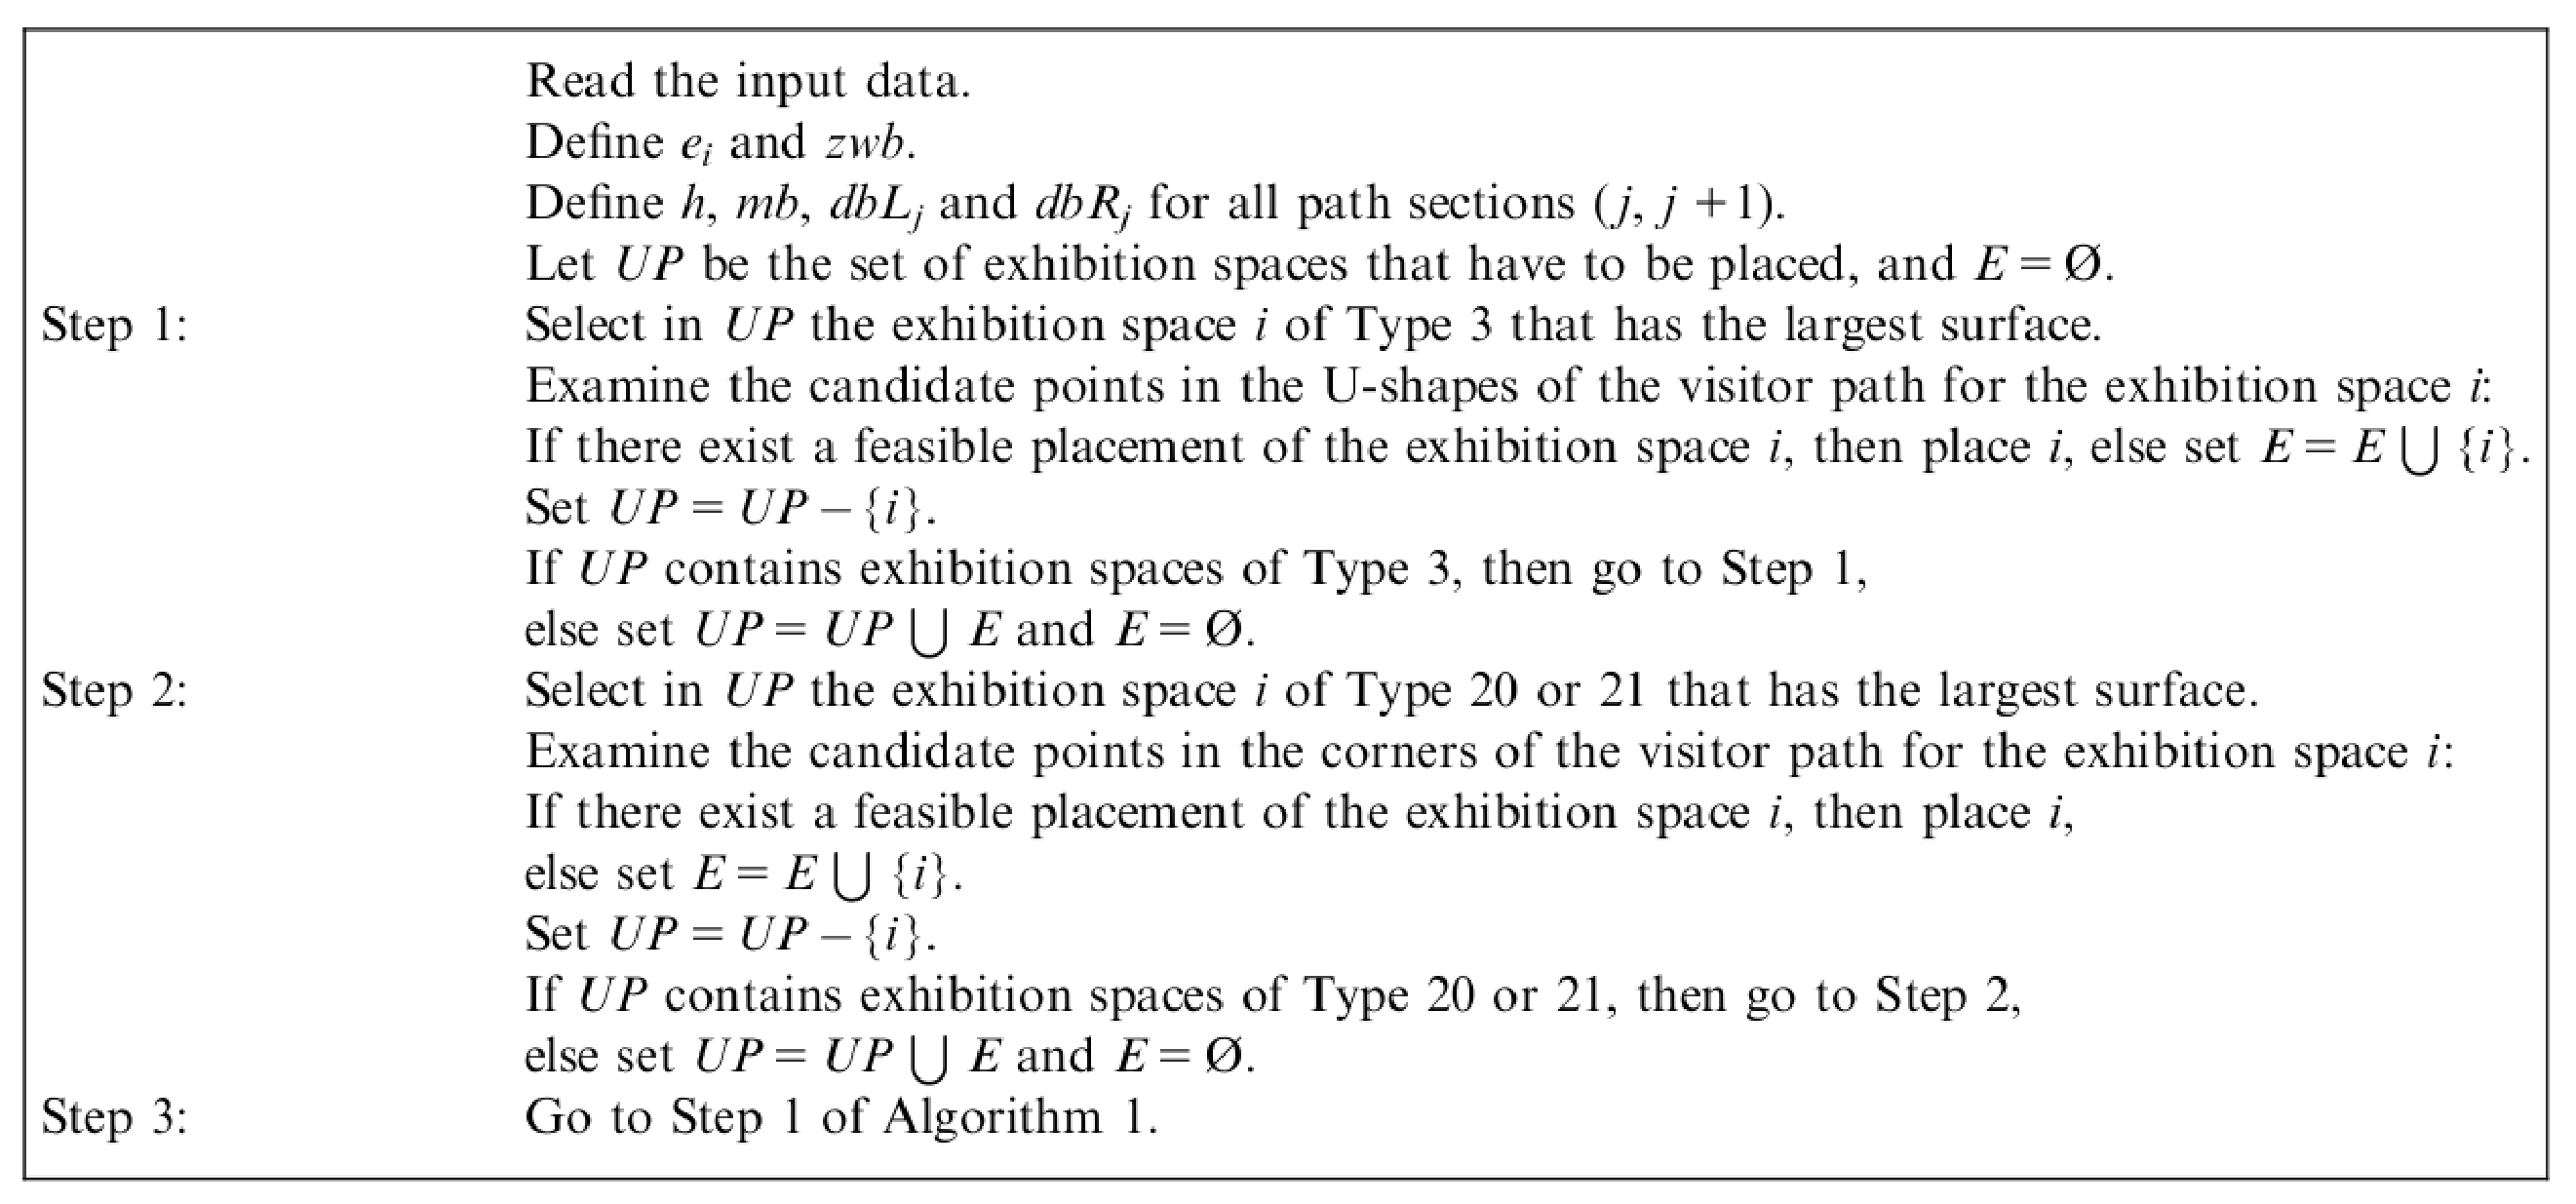
\includegraphics[width=15cm, height=8cm]{images/algo2.eps}
\textit{\caption{\footnotesize Algoritmo 2.}}
\end{figure}
\begin{figure}[h]
\centering
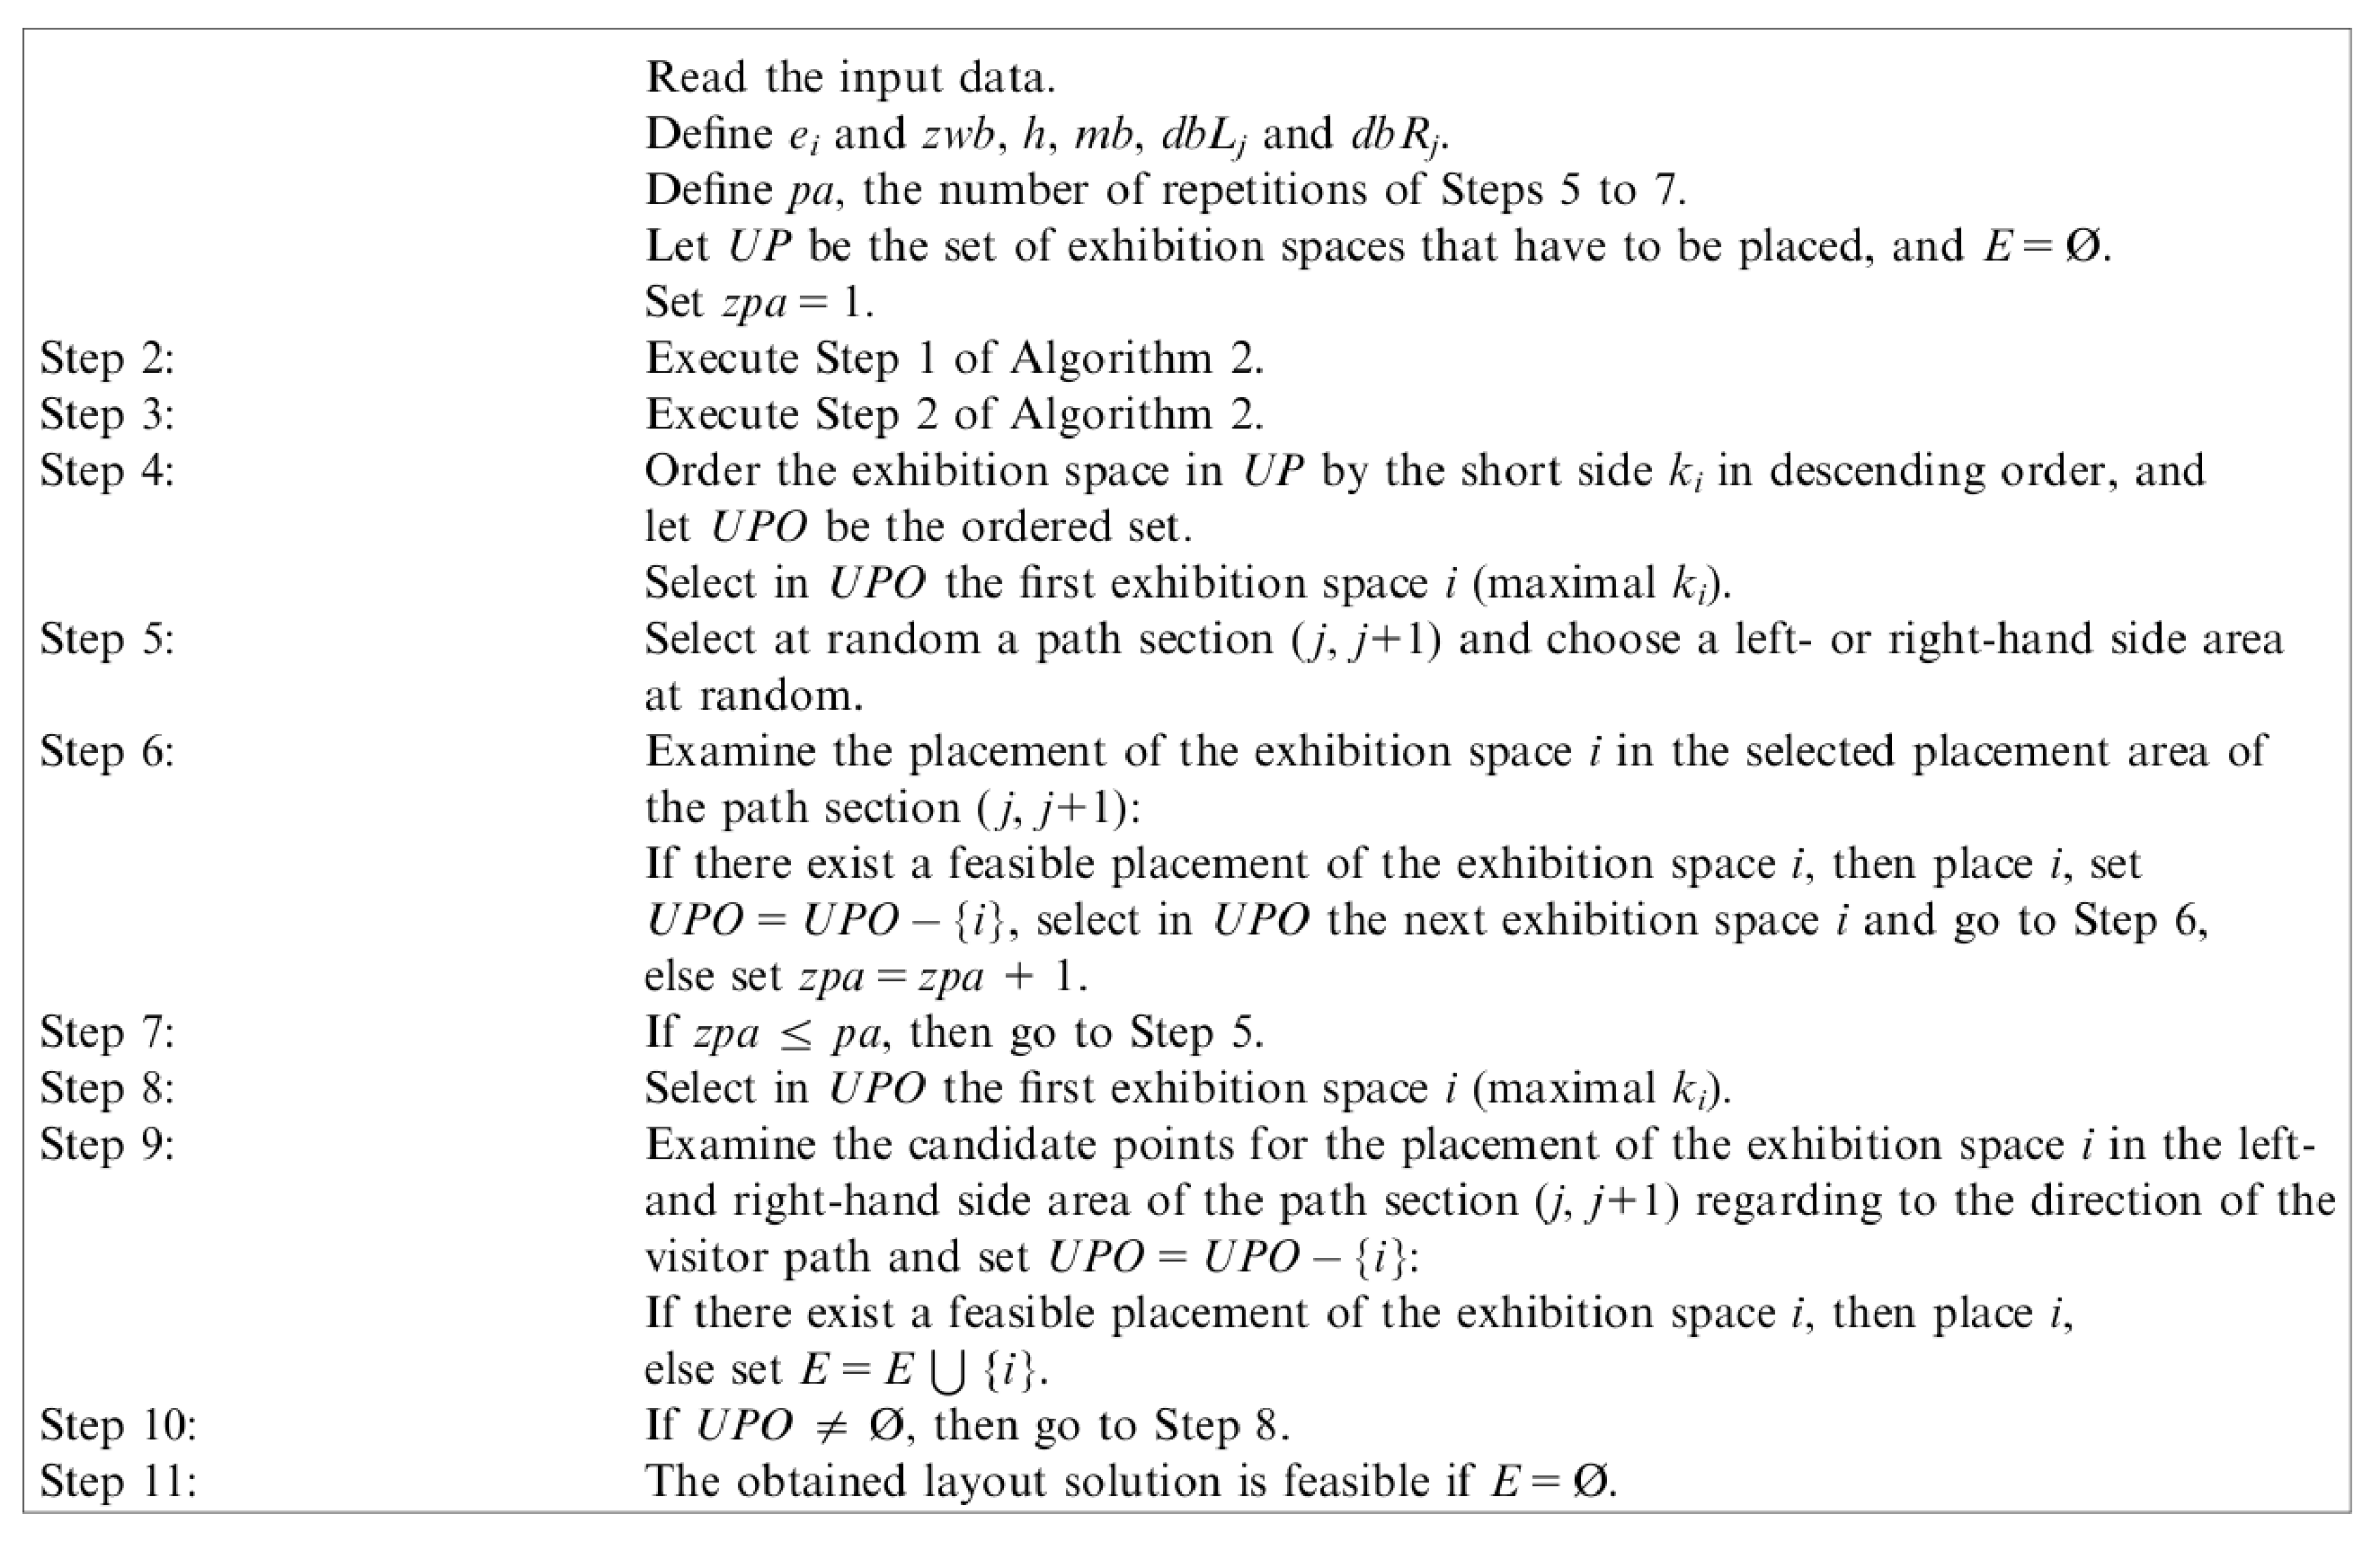
\includegraphics[width=15cm, height=10cm]{images/algo3.eps}
\textit{\caption{\footnotesize Algoritmo 3.}}
\end{figure} 
%%%%%%%%%%%%%%%%%%%%%%%%%%%%FINE SECONDO CAPITOLO%%%%%%%%%%%%%%%%%%%%%%%%%%%%%%%
%%%%%%%%%%%%%%%%%%%%%%%%%%%%%%%%%%%%%%%%%%%%%%%%%%%%%%%%%%%%%%%%%%%%%%%%%
\newpage
\chapter{Casi di studio e specifiche di progetto}                   %crea il capitolo
%%%%%%%%%%%%%%%%%%%%%%%%%%%%%%%%%%%%%%%%%imposta l'intestazione di pagina
Il presente capitolo \`{e} dedicato all'analisi e all'applicazione degli algoritmi esaminati nel primo capitolo, affiancati dal riferimento alle soluzioni viste nel secondo capitolo, in maniera tale da adattare tali conoscenze ai casi di studio presentati qui di seguito.\\
In particolare, tra i dati di interesse fondamentale per l'applicazione dei modelli, si concentrer\`{a} l'attenzione sulle dimensioni degli stand (moduli) e sulle distanze tra di essi, sulla largheza dei corridoi e dei passaggi (\textit{aisles}) secondo il modello di \textit{Fair Layout Optimization Problem} gi\`{a} analizzato, e illustrato nelle figure seguenti:
\begin{figure}[!h]
\centering
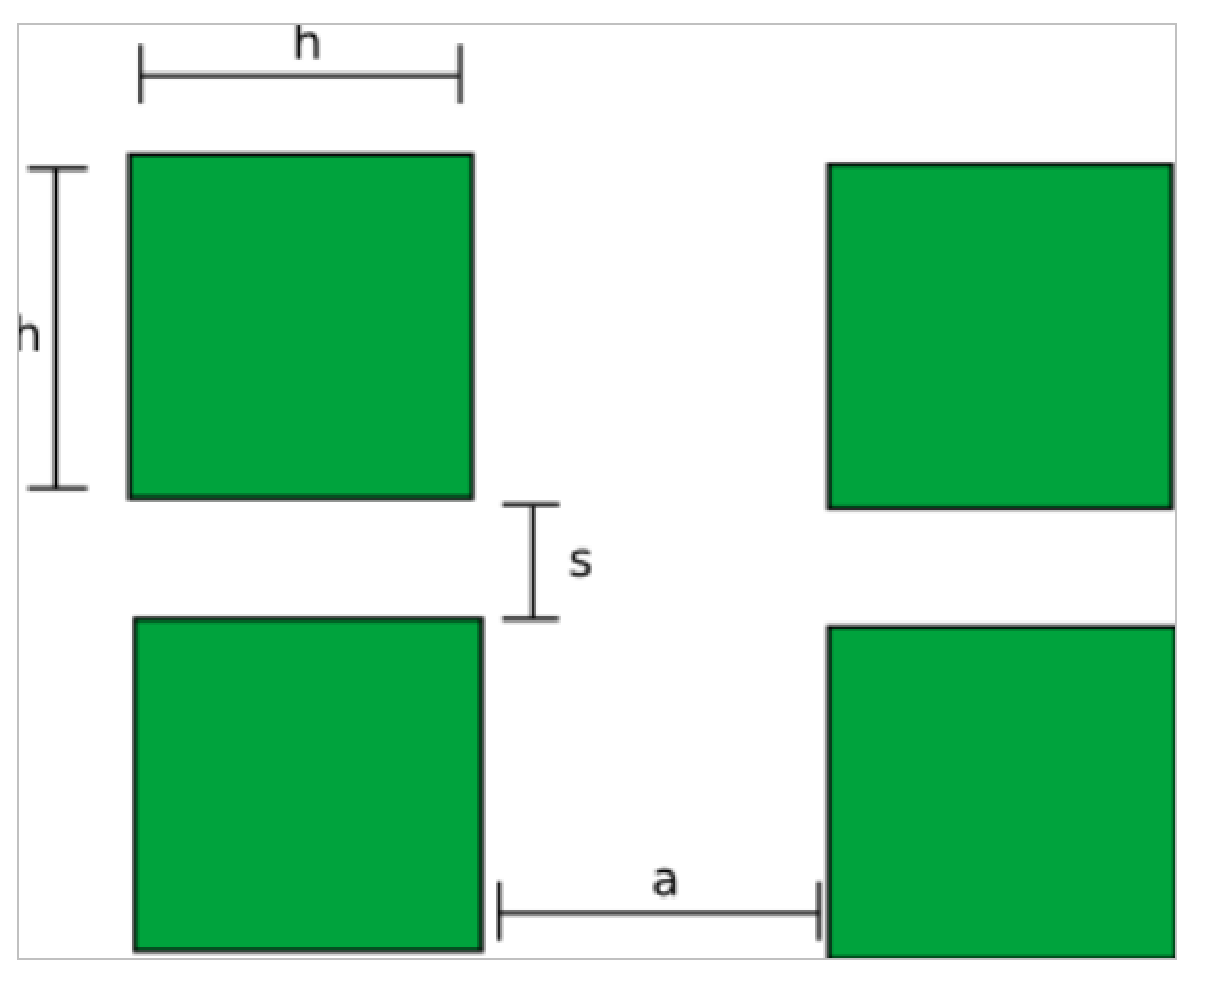
\includegraphics[width=6.5cm, height=5.5cm]{images/moduli2.eps}
\textit{\caption{\footnotesize Flop1, caratteristiche e specifiche di packaging.}}
\end{figure}
\begin{figure}[h]
\centering
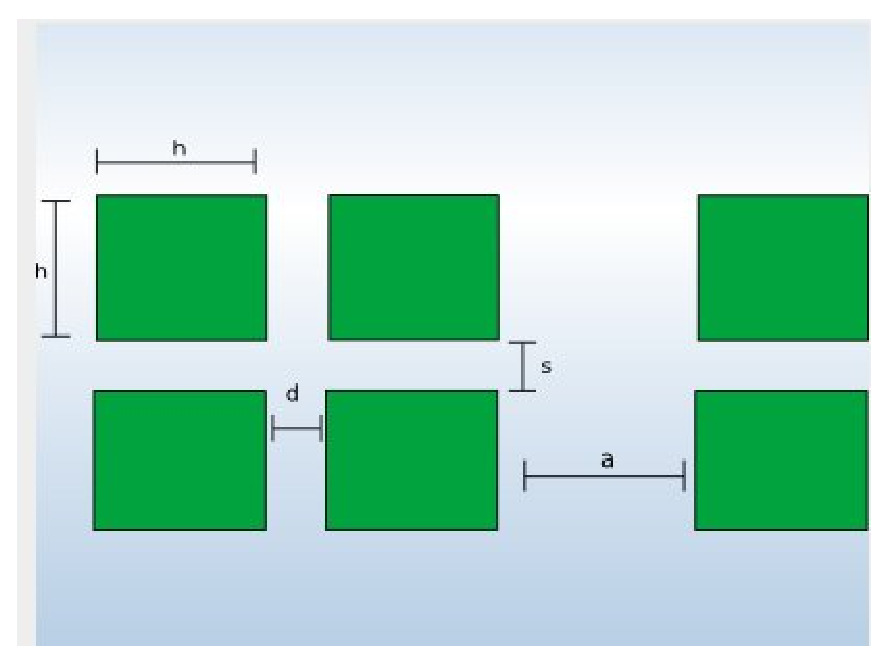
\includegraphics[width=9cm, height=6cm]{images/moduli.eps}
\textit{\caption{\footnotesize Flop2, caratteristiche e specifiche di packaging.}}
\end{figure}
\\
\section{Presentazione dei casi di studio}
I layout fieristici presi in considerazione nel progetto di tesi sono tre:
\begin{itemize}
\item la \textbf{\textit{Fiera del Levante}} di Bari, importantissima e celebre fiera campionaria internazionale che si svolge annualmente nel capoluogo pugliese dal 13 al 21 settembre 2008
\item la Fiera di Bolzano in occasione della \textbf{\textit{fiera mondiale dei veicoli alimentati a gas metano e ad idrogeno}}, che si avr\`{a} luogo dal 9 al 12 Giugno 2008 contemporaneamente al Congresso ENGVA\footnote{European Natural Gas Vehicle Association, associazione europea dei veicoli a gas naturali, come ad esempio metano e idrogeno}
\item l'\textbf{\textit{Expo Ferroviaria 2008}}, fiera dedicata all'industria e alla tecnologia ferroviarie, dal 20 al 22 Maggio 2008 presso il Lingotto Fiere di Torino 
\end{itemize}
I modelli studiati nelle sezioni precedenti sono generalizzabili a vari contesti, per cui il fatto che si analizzino tre differenti contesti non \`{e} altro che una semplice e diretta conferma al concetto di adattare le soluzioni alle varie tipologie di layout che si presentano.

\subsection{Fiera del Levante}
La prima edizione della Fiera del Levante - Campionaria Internazionale - si \`{e} svolta nel 1930, mentre nel 1929 l'Ente Autonomo Fiera del Levante nasceva per iniziativa del Comune di Bari, dell'Amministrazione provinciale e della Camera di Commercio di Bari. La rassegna ha continuato a svolgersi puntualmente a settembre di ogni anno, con la sola interruzione durante gli anni della Seconda Guerra Mondiale, dal 1940 al 1946. Il quartiere fieristico si espande su di una superficie complessiva di circa 300 mila metri quadrati, che ospitano nel corso dell'anno una trentina di manifestazioni alcune delle quali hanno il riconoscimento di internazionalit\`{a}.
\begin{figure}[h]
\centering
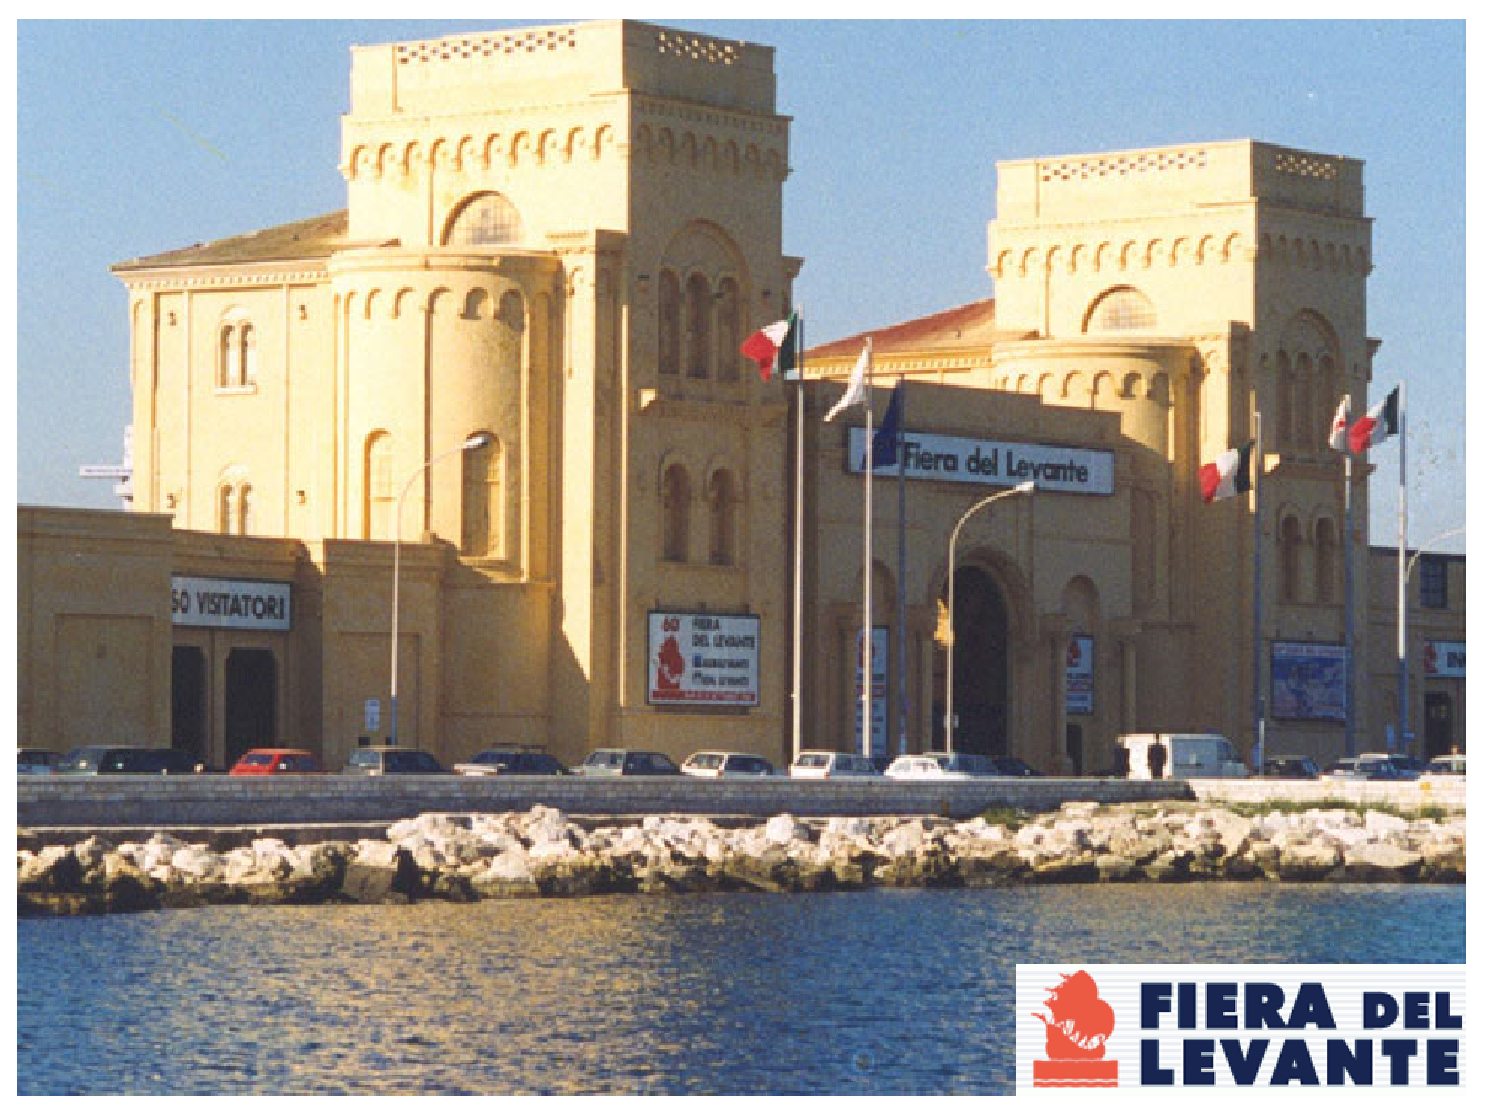
\includegraphics[width=10.5cm, height=7.5cm]{images/levante_panorama.eps}
\textit{\caption{\footnotesize vista panoramica dell'ingresso principale (Ingresso Monumentale) alla Fiera del Levante di Bari.}}
\end{figure}
\\Complessivamente, gli espositori che partecipano annualmente alle manifestazioni in calendario sono oltre 5.000, nazionali ed esteri. A circa due milioni ammontano invece i visitatori. La manifestazione maggiore resta ancora la Campionaria internazionale di settembre, che pu\`{o} contare su oltre 2.000 espositori e pi\`{u} di 700.000 visitatori. La Fiera del Levante opera principalmente al servizio del grande mercato centromeridionale, pur allargando il suo campo operativo al sud est europeo ed all'area mediterranea.\\
Dal punto di vista dei dati tecnici la superficie espositiva, la cui planimetria \`{e} disponibile in figura 3.4, presenta:
\begin{multicols}{2}
\begin{itemize}
\item 44 padiglioni generali
\item 33 padiglioni isolati
\item 7 porte di accesso (ingressi alla fiera)
\item una superficie espositiva complessiva di 300.000 mq
\item una superficie espositiva coperta di 120.000 mq
\item una superficie espositiva scoperta di 40.000 mq 
\end{itemize}
\end{multicols}
\begin{figure}[h]
\centering
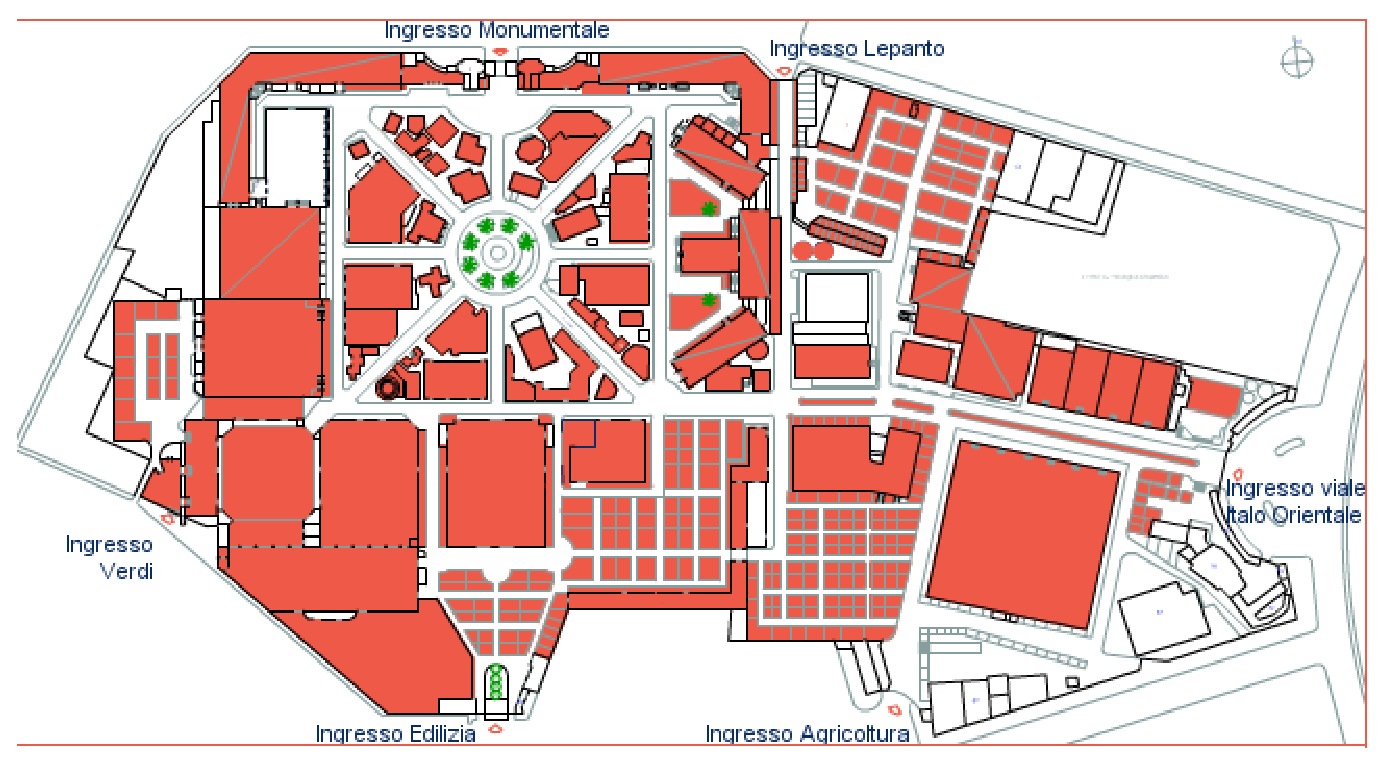
\includegraphics[width=14cm, height=7.3cm]{images/levante_planimetria.eps}
\textit{\caption{\footnotesize planimetria della Fiera del Levante di Bari.}}
\end{figure}
I padiglioni considerati per l'applicazione degli algoritmi sono stati scelti in modo da avere un approccio il pi\`{u} eterogeneo possibile, al fine di coprire le pi\`{u} differenti casistiche: nella fattispecie sono stati presi in esame i padiglioni 11, 116 e 129. Mentre il primo presenta una superficie e una forma regolari, il secondo e il terzo sono molto pi\`{u} irregolari e presentano discontinuit\`{a} nei contorni. 
La scelta di questi spazi espositivi \`{e} appunto giustificata dalle sostanziali differenze tra i tre padiglioni, sia per quanto riguarda la dimensione degli stand, sia per il loro arrangiamento negli spazi previsti.
Dal punto di vista delle dimensioni di interesse per l'applicazione degli algoritmi, di seguito sono elencate le principali caratteristiche di progetto (con riferimento a entrambi i flop e quindi alle figg. 3.1 e 3.2):\\
\begin{table}[h]
\begin{center}
\begin{tabular}{|l|c|r|}
\hline
\textbf{Dim. stand [h $\times$ w]} & \textbf{Largh. corridoi [a]} & \textbf{Dist. tra stand} \\
\hline
\hline
\hline
& \textit{\textbf{\large{Padiglione 11}}} & \\
\hline
4$\times$4 m & 3 m (vert.); 4 m (orizz.) & nessuna \\
\hline
4$\times$3 m & 6.02 m (orizz.) & nessuna \\
\hline
4$\times$3.50 m &  & nessuna \\
\hline
\hline
& \textit{\textbf{\large{Padiglione 116}}} & \\
\hline
4$\times$4 m & 5 m (vert.); 4 m (orizz.) & nessuna \\
\hline
6$\times$6 m &  & nessuna \\
\hline
6$\times$4 m &  & nessuna \\
\hline
\hline
& \textit{\textbf{\large{Padiglione 129}}} & \\
\hline
4$\times$4 m & 5 m (vert.); 4 m (orizz.) & nessuna \\
\hline
6$\times$6 m &  & nessuna \\
\hline
6$\times$4 m &  & nessuna \\
\hline
\end{tabular}
\end{center}
\caption{Caratteristiche e dimensionamenti dei parametri di progetto}
\label{tab:table}
\end{table}
\\Ogni riga rappresenta i diversi dimensionamenti che si trovano all'interno di ciascun padiglione. In particolare non vi \`{e} una sola dimensione degli stand, n\'{e} un'unica alternativa per quanto riguarda la larghezza dei corridoi. Questo \`{e} dovuto, oltre che ad esigenze di spazio, alla forma del padiglione (irregolare o meno che sia) e agli ostacoli strutturali (constraints) che si trovano all'interno degli spazi espositivi.
\begin{figure}[h]
\centering
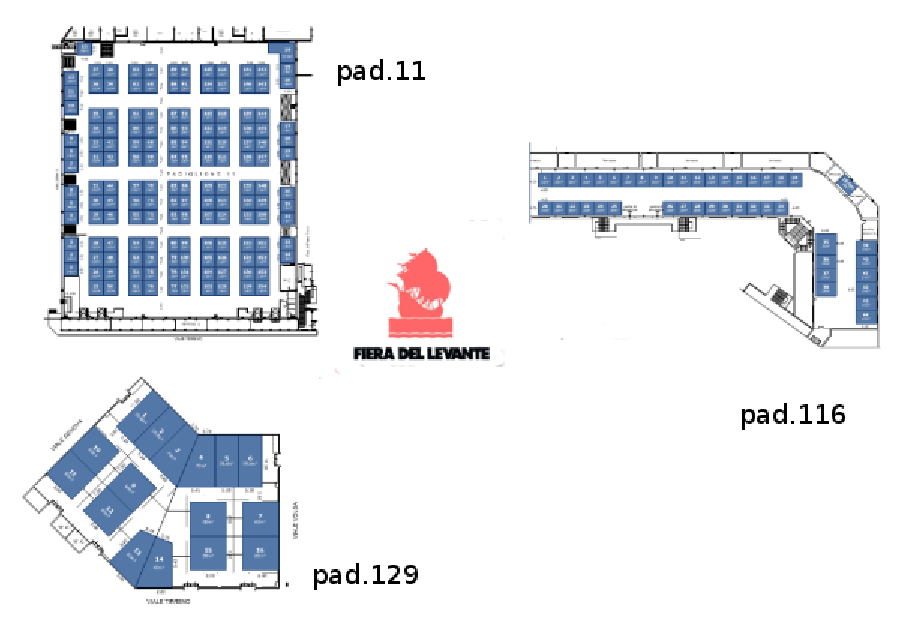
\includegraphics[width=14.5cm, height=9cm]{images/pad_levante.eps}
\textit{\caption{\footnotesize padiglioni della Fiera del Levante considerati nel progetto.}}
\end{figure}
\\Nell'implementare gli algoritmi per questo contesto si terr\`{a} conto di una sola tipologia di dimensioni dei moduli ($[h \times w]$) e dei corridoi ($[a]$), fornendo varie un'unica alternativa progettuale in base ai dati di input standard, imposti dall'organizzazione.
Nelle figura 3.5 sono mostrate le varie planimetrie dei padiglioni considerati, con un arrangiamento degli stands gi\`{a} predisposto per l'edizione 2007.
\\
\subsection{Fiera di Bolzano}
\begin{figure}[h]
\centering
\includegraphics[width=11cm, height=5cm]{images/bolzano_planimetria.eps}
\textit{\caption{\footnotesize organizzazione del quartiere fiersistico Fiera di Bolzano - Messe Bozen.}}
\end{figure}
Da sempre la citt\`{a} di Bolzano, nodo fondamentale tra nord e sud Europa, \`{e} stata sede di fiere e riunioni commerciali e mercantili. Tuttavia la prima fiera campionaria moderna risale al 1948, passando per gli anni '70 in cui si registr\`{o} un notevole sviluppo del quartiere fieristico, e giungendo ai giorni nostri in cui la Fiera di Bolzano \`{e} diventata una Societ\`{a} per Azioni, e ospita nel suo calendario pi\`{u} di 12 manifestazioni annuali di vario genere; si registrano complessivamente circa 171.000 visitatori l'anno.\\
"`"`Fiera Bolzano"'"' si trova al centro della Zona Produttiva Bolzano Sud, solo 2,5 km la separano dal centro citt\`{a}, per cui
il complesso fieristico \`{e} facilmente raggiungibile grazie alla posizione alla periferia. Misura 40.000 mq tra superficie espositiva e annesso centro servizi; se poi si considera anche la struttura polifunzionale adiacente, il "`"`Palaonda"'"', si hanno altri 5000 mq di spazio.  \\
Procedendo con l'analisi dei dati salienti, il quartiere fieristico \`{e} cosituito da 4 padiglioni espositivi, un padiglione polifunzionale (il Palaonda appunto), un Centro Servizi e un Centro Congressi e infine da un Hotel all'interno della fiera; il tutto affiancato da ampi e comodi parcheggi sia interrati che superficiali e rialzati.
L'omogeneit\`{a} delle superfici degli stand consente a tutti gli espositori una presentazione efficace dei propri prodotti e servizi.
In particolare, come si pu\`{o} confrontare anche in figura 3.6, la planimetria del quartiere \`{e} organizzata nel modo seguente:
\begin{multicols}{2}
\begin{itemize}
\item padiglione A - espositivo\\2500 mq
\item padiglione B - espositivo\\4700 mq
\item padiglione C - espositivo\\6060 mq
\item padiglione D - espositivo\\7600 mq
\item padiglione E - polifunzionale\\5000 mq
\item padiglione S - centro servizi
\item padiglione K - centro congressi
\item padiglione H - Hotel Fiera
\end{itemize}
\end{multicols}
Dal 9 al 12 giugno Fiera Bolzano S.p.A. ospiter\`{a} la fiera mondiale dei veicoli alimentati a gas metano e ad idrogeno.
Contemporaneamente si terr\`{a} l'undicesimo Congresso europeo di ENGVA, associazione europea dei veicoli a metano e idrogeno.
La fiera viene organizzata dalla rivista specializzata the Gas Vehicles Report con il sostegno della Provincia Autonoma di Bolzano.
\begin{figure}[h]
\centering
\includegraphics[width=10cm, height=5cm]{images/fierabolzano.eps}
\textit{\caption{\footnotesize immagine a 360 gradi (espansa) del quartiere fiersistico Fiera di Bolzano - Messe Bozen.}}
\end{figure}
\\Al proprio interno il quartiere fieristico possiede un'ampia area stradale riservata agli espositori, ma direttamente  confinante con l'intera costruzione di mostra;  i test drive all'interno di tale struttura costituiscono una prova ulteriore per gli \textit{exhibitors} di mostrare i loro prodotti  in una zona che non richiede agli ospiti di lasciare il centro di mostra. 
\\La manifestazione ENGVA ha luogo all'interno del padiglione D, la cui struttura \`{e} rappresentata in figura 3.9; tale struttura presenta vincoli e \textit{constraints} tipiche, quali aree dedite ai servizi di ristorazione, uscite di emergenza, ingressi e uscite principali, strutture di sostegno (pilastri, ecc.). Nella implementazione dei layout andr\`{a} tenuto conto di tutte queste caratteristiche.\\
Concludendo, si ha quindi che il padiglione D, di dimensioni pari a 7600mq, ospiter\`{a} stand di dimensioni standard (\textit{basic stand}) pari a $5 \times 5$ metri (fig. 3.8), mentre per i corridoi sar\`{a} prevista una larghezza minima di 4 metri. Inoltre saranno distinti due casi, nel primo dei quali la distanza minima tra stand \`{e} nulla, mentre nel secondo \`{e} di 2 metri (sia orizzontale che verticale). 
\begin{table}[h]
\begin{center}
\begin{tabular}{|c|c|c|}
\hline
Dim. stand [$h \times w$] & Largh. corridoi [a] & Dist. tra stand \\
\hline
$5 \times 5$ m & 4 m & nessuna \\
\hline
$5 \times 5$ m & 4 m & 2 m \\
\hline
\end{tabular}
\end{center}
\end{table}
\\
\begin{figure}[h]
\centering
\includegraphics[width=7cm, height=5cm]{images/stand_bolzano.eps}
\textit{\caption{\footnotesize dimensioni standard di uno stand \textit{basic} della Fiera di Bolzano - Messe Bozen.}}
\end{figure} 
\begin{figure}[h]
\centering
\includegraphics[width=10cm, height=8cm]{images/pianobolzano.eps}
\textit{\caption{\footnotesize Padiglione D della Fiera di Bolzano - Messe Bozen.}}
\end{figure}
\\
\newpage
\subsection{Expo Ferroviaria 2008}
La manifestazione torinese \`{e} il punto di incontro per l'industria ferroviaria internazionale, con espositori provenienti da 18 Paesi e specializzati nei pi\`{u} svariati campi dell'industria e della tecnologia che hanno a che vedere col mondo delle ferrovie.
L'unica fiera ferroviaria che ha luogo regolarmente in Italia si svolge a Torino presso il Lingotto Fiere dal 20 al 22 maggio 2008.
Strutturalmente l'Expo ospitata al Lingotto Fiere si suddivide in due padiglioni, i quali hanno le seguenti dimensioni:
\begin{multicols}{2}
\underline{Padiglione1}\\dimensioni: 141 $\times$ 54 metri\\totale: 7620 mq;\\altezza max: 10,5 metri;\\
\underline{Padiglione2}\\dimensioni: 187 $\times$ 96 metri\\totale: 17960 mq;\\altezza max: 14,2 metri;
\end{multicols}
\begin{figure}[h]
\centering
\includegraphics[width=11.5cm, height=6cm]{images/stand_expo.eps}
\textit{\caption{\footnotesize dimensioni dello stand standard considerato per l'Expo Ferroviaria 2008.}}
\end{figure}
\begin{figure}[h]
\centering
\includegraphics[width=6.5cm, height=9cm]{images/lingotto.eps}
\textit{\caption{\footnotesize panoramica del quartiere Lingotto Fiere di Torino sede dell'Expo Ferroviaria 2008.}}
\end{figure}
Per quanto riguarda i dati inerenti gli spazi espositivi, considerando lo stand di figura 3.10, le dimensioni standard sono di $[h \times w] = 4 \times 4$ metri; per ci\`{o} che concerne le larghezze dei corridoi, invece, le dimensioni del parametro $[a]$ sono di 3 metri; si \`{e} scelto, per evitare complicazioni al modello e perch\'{e} non indispensabili, di non considerare rilevanti (e quidi nulle) le distanze tra i singoli moduli. 
\begin{table}[h]
\begin{center}
\begin{tabular}{|c|c|c|}
\hline
Dim. stand [$h \times w$] & Largh. corridoi [a] & Dist. tra stand \\
\hline
$4 \times 4$ m & 3 m & nessuna \\
\hline
\end{tabular}
\end{center}
\end{table}
\\In figura 3.13 \`{e} riportata la planimetria della manifestazione di Torino. \\  
\begin{figure}[h]
\centering
\includegraphics[width=16cm, height=9.5cm]{images/lingotto_plan.eps}
\textit{\caption{\footnotesize planimetria del quartiere Lingotto Fiere di Torino. In rosso sono sottolineati i padiglioni sede dell'Expo Ferroviaria 2008.}}
\end{figure}
\begin{figure}[h]
\centering
\includegraphics[width=14.5cm, height=21cm]{images/pad_expo2008.eps}
\textit{\caption{\footnotesize padiglioni della Expo Ferroviaria 2008. I due padiglioni sono separati dai muri portanti (in nero). Nella parte alta del secondo padiglione \`{e} stata tagliata la zona di ristorazione, comunque inutile al layout. La figura comprende solamente le zone idonee al contenimento degli stand.}}
\end{figure}
\\
\section{Criterio per la definizione e la scrittura delle matrici}
Riprendiamo un argomento gi\`{a} trattato, ma comunque di fondamentale rilievo per l'implementazione degli algoritmi e dei modelli appena visti.\\
Si crei una matrice $\Phi$, composta da quadrati di dimensione $[\delta \times \delta]$ che copra totalmente il rettangolo di dimensioni $[H \times W]$ contenente la superficie di esposizione. Usando un approccio granulare, si esprimeranno tutte le dimensioni (quelle esterne e degli stand) come multipli di questi (piccoli) valori. In particolare \`{e} definita la seguente dimensione:
$$X_{\delta} = \dfrac{X}{\delta}$$
dove $X =\left\lbrace H, W, h, w\right\rbrace $. Tale matrice ha perci\`{o} dimensioni $\lfloor W_{\delta} \times H_{\delta}\rfloor$. Un elemento della matrice assume valore 1 se il corrispondente quadratino $[\delta \times \delta]$ pu\`{o} essere usato completamente per l'impaccamento degli stand:
$$ 
\Phi_{i,j} =  
\left\{
\begin{array}{rl}
1 & \mbox{se il quadrato } (i, j) \mbox{ pu\`{o} essere interamente usato per il package}\\
0 & \mbox{altrimenti}
\end{array}
\right.
$$
questo $\forall j = 1,...,W_{\delta}$ e $\forall i = 1,...,H_{\delta}$. 
\\Si noti che per $\delta << W$, o ancora meglio per $\delta << w$, l'approssimazione risulta molto bassa. \\
Ora si numerino le colonne da 1 a $W_{\delta}$ . Si dir\`{a} che una colonna \`{e} scelta per l'impaccamento, se una striscia di stand \`{e} piazzata con l'angolo sinistro dello stand all'inizio della colonna. A causa del criterio utilizzato e per evitare di dover costruire matrici in input di notevoli dimensioni \`{e} stata usata l'approssimazione al metro (ogni quadratino corrisponde ad un mq). Di questa approssimazione ne risentono ad esempio le dimensioni delle porte che a volte possono raggiungere la larghezza di 2 metri. 
Si ricordi che, dato un modello, la soluzione del corrispondente rilassamento lineare \`{e} sempre intera se tutta la parte destra del modello \`{e} intera e se la matrice dei vincoli \`{e} totalmente unimodulare\footnote{una matrice totalmente unimodulare \`{e} una matrice (non necessariamente quadrata) per la quale anche ogni minore non singolare \`{e} unimodulare. Ne consegue che ogni suo elemento vale $0$, $+1$ o $-1$. Un programma intero nel quale la matrice dei vincoli \`{e} totalmente unimodulare pu\`{o} essere risolto efficientemente, in quanto il suo rilassamento LP porta a soluzioni intere.} (TUM).

\chapter{Implementazione degli algoritmi e risultati computazionali}                   %crea il capitolo
%%%%%%%%%%%%%%%%%%%%%%%%%%%%%%%%%%%%%%%%%imposta l'intestazione di pagina
Questo capitolo \`{e} dedicato all'applicazione specifica degli algoritmi presentati nel capitolo 1 ai casi di studio presentati nel capitolo precedente. Partendo dalle planimetrie delle fiere di Bari, Bolzano e Torino, sono stati implementati gli algoritmi tramite un software sviluppato su piattaforma Java dall'Ing.Muritiba, presso il DEIS\footnote{Dipartimento di Elettronica, Informatica e Sistemistica} di Bologna. \\Tale applicativo \`{e} in grado di fornire soluzioni per l'impaccamento del maggior numero possibile di stand. Il software lavora costruendo le piantine dei padiglioni attraverso delle coordinate che vengono fornite come input; il concetto base \`{e} quello di creare un poligono esterno con la forma del padiglione e successivamente creare dei piccoli poligoni interni che evidenzino le aree in cui non \`{e} possibile impaccare gli stand (a causa di porte, bar, servizi, ecc.).
\\Per creare questi poligoni \`{e} necessario fornire le coordinate $X-Y$ di ogni angolo partendo da un punto, ed elencare successivamente tutti i restanti punti in senso orario o in senso antiorario. I poligoni sono divisi in due tipi:
\begin{itemize}
\item \underline{polygon unlock} - \`{e} il poligono che rappresenta la forma del padiglione o di ci\`{o} che voglio rappresentare; pu\`{o} essere uno solo
\item \underline{polygon lock} - rappresenta ogni singola area in cui non \`{e} possibile impaccare alcuno stand ed \`{e} evidente che all'interno di un'area espositiva ne troveremo di diversi tipi
\end{itemize}
Come si vedr\`{a} poi meglio nello studio dei singoli casi reali, la forma degli spazi espositivi e dei corridoi \`{e} rappresentata in bianco mentre tutti i vincoli (polygon lock) sono rappresentati da spazi grigi.
Una volta introdotti questi dati in input si \`{e} poi provveduto alle implementazioni di due diversi FLOP\footnote{acronimo per indicare il Fair Layout Optimization Problem} per calcolare quanti stand poter inserire all'interno dei nostri padiglioni.  
Per ogni planimetria sono stati eseguiti entrambi i FLOP, le cui caratteristiche sono richiamate brevemente di seguito:
\begin{description}
\item[Flop1]: si tratta di singoli strip di stand di forma quadrata dove vengono forniti in input i valori di $h$ (lato dello stand), $s$ (piccoli corridoi di separazione tra gli stand) ed $a$ (distanza tra gli strip di stand). Specifichiamo per\`{o} che $s$ \`{e} sempre stato considerato nullo in entrambi i FLOP per ciascuna soluzione
\item[Flop2]: si tratta di doppi strip di stand dove vengono forniti in input gli stessi dati del FLOP1; in pi\`{u} compare un dato $d$ che per\`{o} negli studi presentati di seguito sar\`{a} sempre considerato nullo
\end{description}
Con riferimento ai casi di studio proposti, verranno presentate di seguito le varie soluzioni relative all'implementazione degli algoritmi e dei \textit{flop} ai vari padiglioni. \\Si sottolinea che la procedura di implementazione degli algoritmi, per ciascuna soluzione, \`{e} stata effettuata su macchine costituite da processore Intel Core 2 Duo con 1GB di memoria RAM e sistema operativo Linux Ubuntu su cui \`{e} installata la Java Virtual Machine.  

\section{Fiera del Levante: soluzione}
Con riferimento al padiglione 11 e alle dimensioni rappresentate nella tabella 3.1, presentiamo le soluzioni relative, prima impiegando il FLOP1 e quindi il FLOP2:
\begin{table}[h]
\begin{center}
\begin{tabular}{|l|l|l|l|}
\hline
CPU-time FLOP1 & CPU-time FLOP2 & Stands FLOP1 & Stands FLOP2 \\
\hline
215 ms & 680 ms & 89 & 114 \\
\hline
\end{tabular}
\end{center}
\end{table}
\\Ricordiamo che nelle ipotesi abbiamo considerato i moduli di dimensione standard $4 \times 4$ metri e i corridoi di larghezza 4 metri in linea orizzontale e 3 metri in verticale, tralasciando gli altri casi poich\'{e} la soluzione attuale rappresenta il miglior compromesso tra spazi occupati e numero di stand ottimo. In figura 4.1 sono rappresentate le soluzioni relative al Padiglione 11.
\begin{figure}[h]
\centering
\includegraphics[width=12cm, height=8cm]{images/pab11.eps}
\textit{\caption{\footnotesize soluzioni proposte per il padiglione 11 con FLOP1 e FLOP2.}}
\end{figure}
\\Per quanto riguarda il padiglione 116, sempre con riferimento alla tabella 3.1, si riportano entrambe le soluzioni adottate:
\begin{table}[h]
\begin{center}
\begin{tabular}{|l|l|l|l|}
\hline
CPU-time FLOP1 & CPU-time FLOP2 & Stands FLOP1 & Stands FLOP2 \\
\hline
158 ms & 351 ms & 27 & 31 \\
\hline
\end{tabular}
\end{center}
\end{table}
\\In figura 4.2 sono riportate le rispettive grafiche dei FLOP.
\begin{figure}[h]
\centering
\includegraphics[width=12cm, height=8cm]{images/pab116.eps}
\textit{\caption{\footnotesize soluzioni proposte per il padiglione 116 con FLOP1 e FLOP2. In questo caso gli stand sono rappresentati in nero e i vincoli sempre in grigio.}}
\end{figure}
\\In questo padiglione le dimensioni relative alla dimensione dei moduli sono sempre di $4 \times 4$ metri, mentre i corridoi hanno dimensione di 5 (verticale) $\times$ 4 (orizzontale) metri.\\  
Prendiamo infine in considerazione infine il Padiglione 129, di forma piuttosto irregolare analogamente al caso precedente, e riportiamo le soluzioni nella tabella seguente e nella figura 4.3:
\begin{table}[h]
\begin{center}
\begin{tabular}{|l|l|l|l|}
\hline
CPU-time FLOP1 & CPU-time FLOP2 & Stands FLOP1 & Stands FLOP2 \\
\hline
106 ms & 272 ms & 24 & 31 \\
\hline
\end{tabular}
\end{center}
\end{table}
\\dove, come per i precedenti padiglioni, la dimensione degli stand \`{e} di $4 \times 4$ metri e per i corridoi \`{e} di 5 (verticale) $\times$ 4 (orizzontale) metri.
\begin{figure}[h]
\centering
\includegraphics[width=12cm, height=12cm]{images/pab129.eps}
\textit{\caption{\footnotesize soluzioni proposte per il padiglione 129 con FLOP1 e FLOP2. In questo caso gli stand sono rappresentati in nero e i vincoli sempre in grigio.}}
\end{figure}
\\Nel listato seguente sono elencati i file di input da fornire al software Java per costruire il layout di ciascun padiglione (rispettivamente, i padiglioni 11, 116 e 129), tenendo in considerazione i vincoli e gli ostacoli imposti dal contesto:
\begin{verbatim}
polygon; unlock; 0 0; 0 80; 70 80; 70 0			
lock1; lock; 0 0; 0 8; 4 8; 4 0					
lock2; lock; 0 18.5; 0 22.5; 4 22.5; 4 18.5
lock3; lock; 0 33; 0 37; 4 37; 4 33
lock4; lock; 0 47.5; 0 52; 4 52; 4 47.5
lock5; lock; 0 64; 0 78; 4 78; 4 64
lock6; lock; 66 0; 66 12; 70 12; 70 0
lock7; lock; 66 20; 66 24; 70 24; 70 20
lock8; lock; 66 34.5; 66 42.5; 70 42.5; 66 34.5
lock10; lock; 66 53; 66 63; 70 63; 70 53
lock11; lock; 12 80; 12 75; 16 75; 16 80
\end{verbatim}
\begin{verbatim}
polygon; unlock; 0 0; 0 84; 16 100; 48 100; 48 81; 22 81; 18 78; 18 0					
lock1; lock; 0 0; 0 84; 16 100; 24 100; 24 92; 18 92; 14 90; 6 84; 4 76; 4 0					
lock2; lock; 48 81; 32 81; 32 87; 48 87
lock3; lock; 18 26; 14 26; 14 38; 18 38
lock4; lock; 18 92; 22 92; 22 90; 18 90
\end{verbatim}
\begin{verbatim}
polygon; unlock; 0 0; 0 31,2; 22 53.2; 46 30; 33.6 18; 33.6 0			
lock1; lock; 0 6.4; 0 12; 3 12; 3 6.4					
lock2; lock; 0 20.8; 0 26.4; 3 26.4; 3 20.8
lock3; lock; 8 38; 22 53.2; 24 51.2; 10 36; 8 36;
lock4; lock; 46 30; 43.2 27.2; 36 34; 38 37.2
\end{verbatim}

\section{Fiera di Bolzano: soluzione}
Avendo precedentemente considerato la forma degli stand di $5 \times 5$ metri e la larghezza di tutti i corridoi di 4 metri (sia in orizzontale che in verticale), la soluzione presentata per il padiglione D della Fiera di Bolzano \`{e} riassunta nella tabella che segue:
\begin{table}[!h]
\begin{center}
\begin{tabular}{|l|l|l|l|l|}
\hline
& CPU-time FLOP1 & CPU-time FLOP2 & Stands FLOP1 & Stands FLOP2 \\
\hline
caso1& 230 ms & 710 ms & 112 & 126 \\
\hline
caso2& 275 ms & 800 ms & 94 & 100 \\
\hline
\end{tabular}
\end{center}
\end{table}
\\In questa rappresentazione sono stati prese in considerazione due varianti: nel primo caso (caso 1) la distanza imposta tra gli stands \`{e} nulla, mentre nel secondo (caso 2) \`{e} di 2 metri sia in orizzontale che in verticale. Per il resto tutti i parametri rimangono invariati.\\ 
Analogamente a quanto fatto per il contesto precedente, viene qui di seguito presentato il listato relativo al contesto di Bolzano coi rispettivi \textit{lock} che rappresentano i vincoli e gli ostacoli all'interno del padiglione:
\begin{verbatim}
polygon; unlock; 0 0; 0 80; 85 80; 85 0				
lock1; lock; 0 0; 0 30; 13 30; 13 0
lock2; lock; 14 0; 14 5; 19 5; 19 0
lock3; lock; 33 0; 33 5; 38 5; 38 0
lock4; lock; 52 0; 52 5; 57 5; 57 0
lock5; lock; 71 0; 71 5; 76 5; 76 0
lock6; lock; 0 30; 0 35; 5 35; 5 30
lock7; lock; 0 44; 0 49; 5 49; 5 44
lock8; lock; 0 63; 0 68; 5 68; 5 63
lock9; lock; 13 80; 20 80; 20 74; 13 74
lock10; lock; 51 80; 58 80; 58 74; 51 74
lock11; lock; 23 5; 23 7.5; 25.5 7.5; 25.5 5
lock12; lock; 41.5 5; 41.5 7.5; 44 7.5; 44 5
lock13; lock; 60 5; 60 7.5; 62.5 7.5; 62.5 5
lock14; lock 78.5 5; 78.5 7.5; 80 7.5; 80 5
lock15; lock; 78.5 24; 78.5 26.5; 80 26.5; 80 24
lock16; lock; 78.5 41.5; 78.5 44; 80 44; 80 41.5
lock17; lock; 78.5 59; 78.5 61.5; 80 61.5; 80 59
\end{verbatim}

\section{Expo Ferroviaria 2008: soluzione}
Il calcolo degli elementi e degli spazi per i padiglioni dell'Expo Ferroviaria 2008 hanno portato ad una soluzione ottimizzata che viene riassunta nella tabella seguente:
\begin{table}[h]
\begin{center}
\begin{tabular}{|c|c|c|c|}
\hline
CPU-time FLOP1 & CPU-time FLOP2 & Stands FLOP1 & Stands FLOP2 \\
\hline 
174 ms & 478 ms & 264 & 374 \\
\hline 
371 ms & 1046 ms & 578 & 781 \\
\hline
\end{tabular}
\end{center}
\caption{Risultati dei calcoli per i padiglioni dell'Expo Ferroviaria 2008. In alto i dati riguardanti il pad.1 e in basso quelli per il pad.2.}
\label{tab:table}
\end{table}
\\mentre per quanto riguarda le immagini relative ad entrambi i padiglioni, esse sono rappresentate nelle figure 4.4 e 4.5
\begin{figure}[h]
\centering
\includegraphics[width=10cm, height=14cm]{images/pad1_expo.eps}
\textit{\caption{\footnotesize soluzioni proposte per il padiglione 1 dell'Expo Ferroviaria con FLOP1 e FLOP2 rispettivamente a sinista e a destra.}}
\end{figure}
\begin{figure}[h]
\centering
\includegraphics[width=12cm, height=14cm]{images/pad2_expo.eps}
\textit{\caption{\footnotesize soluzioni proposte per il padiglione 2 dell'Expo Ferroviaria con FLOP1 e FLOP2 rispettivamente a sinista e a destra.}}
\end{figure}
Ricordiamo che, per entrambi i padiglioni, le dimensioni dei moduli sono di $4 \times 4$ metri, mentre i corridoi hanno una larghezza di 3 metri.
\\Presentiamo infine i file di input che permettono la mappatura dei due padiglioni dell'Expo Ferroviaria:
\begin{verbatim}
polygon; unlock; 0 0; 0 153; 54 153; 54 0					
lock1; lock; 0 0; 0 12.5; 54 12.5; 54 0 					
lock2; lock; 0 12; 0 16; 31 16; 31 12 						
lock3; lock; 0 20; 0 27.92; 4 27.92; 4 20 					
lock4; lock; 0 35.84; 0 38.34; 2.5 38.34; 2.5 35.84		
lock5; lock; 0 45.34; 0 53.26; 4 53.26; 4 45.34			
lock6; lock; 0 60.26; 0 62.76; 2.5 62.26; 2.5 60.26    		
lock7; lock; 0 69.26; 0 77.18; 54 77.18; 54 69.26				
lock8; lock; 0 83.68; 0 86.18; 2.5 86.18; 2.5 83.68			
lock9; lock; 0 93.18; 0 101.1; 4 101.1; 4 93.18				
lock10; lock; 0 107.6; 0 110.1; 2.5 110.1; 2.5 107.6			
lock11; lock; 0 116.6; 0 124.52; 54 124.52; 54 116.6			
lock12; lock; 0 128.52; 0 153; 24.48 153; 24.48 128.52		
lock13; lock; 51.5 153; 54 153; 54 150.5; 51.5 150.5		
lock14; lock; 51.5 133.52; 54 133.52; 54 131.02; 51.5 131.02
lock15; lock; 51.5 110.1; 54 110.1; 54 107.6; 51.5 107.6
lock16; lock; 51.5 86.18; 54 86.18; 54 83.68; 51.5 83.6
lock17; lock; 51.5 62.76; 54 62.76; 54 60.26; 51.5 60.26
lock18; lock; 51.5 38.34; 54 38.34; 54 35.84; 51.5 35.84
\end{verbatim} 
\begin{verbatim}
polygon; unlock; 0 0; 0 199; 96 199; 96 0
lock1; lock; 0 0; 0 12.5; 96 12.5; 96 0				
lock2; lock; 0 199; 96 199; 96 124.52; 60 124.52; 60 174.52; 0 174.52
lock3; lock; 0 116.6; 0 124.52; 96 124.52; 96 116.6		
lock4; lock; 0 69.26; 0 77.18; 96 77.18; 96 69.26
\end{verbatim}
\section{Considerazioni finali}
Rispetto all'arrangiamento degli spazi effettuato dagli organizzatori, i risultati ottenuti mediante calcoli e modelli matematici hanno portato ad un miglioramento e ad un'ottimizzazione in termini di stand impiegati e di vincoli rispettati, il tutto in accordo con le specifiche mostrate nel terzo capitolo.\\
In particolare, per quanto riguarda le tre alternative e i tre layout analizzati, si sono riscontrati i risultati complessivi schematizzati in tabella 4.2\\
\begin{table}[!h]
\begin{center}
\begin{tabular}{|l|c|c|c|c|}
\hline
 & \textbf{Stands originali} & \textbf{Stands FLOP1} & \textbf{Stands FLOP2} \\
\hline
\hline
Padiglione 11\\Fiera del Levante & 154 & 89 & 114 \\
\hline
Padiglione 116\\Fiera del Levante & 45 & 27 & 31 \\
\hline
Padiglione 129\\Fiera del Levante & 16 & 24 & 31 \\
\hline
Padiglione D.1\\Fiera di Bolzano & 90 & 112 & 126  \\
\hline
Padiglione D.2\\Fiera di Bolzano & 90 & 94 & 100  \\
\hline
Padiglione 1\\Expo Ferroviaria & 114 & 274 & 374 \\
\hline
Padiglione 2\\Expo Ferroviaria & 219 & 578 & 781 \\
\hline
\hline
\end{tabular}
\end{center}
\caption{Numero di stands per ogni layout analizzato, in relazione agli stand disposti dagli organizzatori nella configurazione originale di ciascun padiglione. Si noti che il padiglione D del contesto di Bolzano \`{e} stato suddiviso in due parti a seconda dei casi enunciati nel paragrafo 4.2}
\label{tab:table}
\end{table}
\\Oltre ai dati relativi al numero di stands "`"`impacchettati"'"' e alle elaborazioni computazionali, ricopre fondamentale importanza e rilevanza il dato relativo alla dimensione delle matrici associate ai vari FLOP.
\\In particolare, rimandando il lettore al paragrafo 3.2, le matrici create conseguentemente alle elaborazioni sono, per ciascuna delle manifestazioni fieristiche considerate, le seguenti:
\begin{table}[h]
\begin{center}
\begin{tabular}{|c|c|c|}
\hline
Matrix Pad. 11 & Matrix Pad. 116 & Matrix Pad. 129 \\
\hline
[799 x 699] & [999 x 479] & [531 x 459] \\
\hline
\end{tabular}
\end{center}
\caption{Dimensione delle matrici per la Fiera del Levante}
\label{tab:table}
\end{table} 
\begin{table}[h]
\begin{center}
\begin{tabular}{|c|c|}
\hline
Matrix Pad. D.1 & Matrix Pad. D.2 \\
\hline
[749 x 639] & [819 x 669] \\
\hline
\end{tabular}
\end{center}
\caption{Dimensione delle matrici per la Fiera di Bolzano - Messe Bozen con le due soluzioni in base alla distanza tra i moduli}
\label{tab:table}
\end{table} 
\begin{table}[h]
\begin{center}
\begin{tabular}{|c|c|}
\hline
Matrix Pad. 1 & Matrix Pad. 2 \\
\hline
[1529 x 539] & [1989 x 959] \\
\hline
\end{tabular}
\end{center}
\caption{Dimensione delle matrici per l'Expo Ferroviaria 2008}
\label{tab:table}
\end{table} 
%%%%%%%%%%%%%%%%%%%%%%%%%%%%FINE QUARTO CAPITOLO%%%%%%%%%%%%%%%%%%%%%%%%%%%%%%%
%%%%%%%%%%%%%%%%%%%%%%%%%%%%%%%%%%%%%%%%%%%%%%%%%%%%%%%%%%%%%%%%%%%%%%%%%
\newpage
\chapter{Conclusioni}                   %crea il capitolo
%%%%%%%%%%%%%%%%%%%%%%%%%%%%%%%%%%%%%%%%%imposta l'intestazione di pagina
Prima di parlare degli obiettivi raggiunti, \`{e} bene ripercorrere velocemente tutta la strada fatta. Dopo aver individuato nel FLOP (Fair Layout Optimization Problem) il cuore della tesi, si \`{e} intrapreso un percorso di ricerca nella letteratura, dapprima in ambito logistico e poi nell'area della ricerca operativa, allo scopo di trovare qualche supporto bibliografico significativo. In ambito logistico sono stati trovati solo testi inerenti al layout industriale, ma pochissimi testi focalizzato sul layout fieristico. Anche per quanto riguarda l'ambito della ricerca operativa, non sono state trovate pubblicazioni indirizzate al FLOP, ma sono comunque stati trovati problemi simili. Il problema del posizionamento di stand pu\`{o} essere infatti visto come caso particolare dei problemi di impaccamento rivolti ad altri oggetti (cui possiamo ricondurre gli stands); un ampio capitolo della tesi \`{e} infatti incentrato sui problemi di Knapsack, di Cutting e di Packing.
La ricerca bibliografica ha portato alla scoperta di un altro problema gi\`{a} ampiamente discusso in letteratura e che si avvicina a quello della tesi; si tratta del Facility Layout Problem (FLP). In particolare una tipologia particolare di quest'ultimo, ovvero il Quadratic Assignement Problem (QAP), presenta caratteri molto simili agli ultimi modelli presentati nel capitolo 3. Se da un lato gli algoritmi studiati per il FLP possono essere prese come riferimento e come spunto per alcuni sviluppi futuri del FLOP, non potranno mai essere presi in toto, poich\'{e} nei primi vi \`{e} il flusso tra una posizione e l'altra come \textit{driver} principale, mentre nel secondo non vi \`{e} alcun problema di movimentazione di materiali.\\
Una volta finita la parte di ricerca bibliografica sono stati affrontati i modelli per la risoluzione del FLOP; questi ultimi sono stati prima analizzati nel capitolo 3 e poi inseriti nei contesti presentati nel capitolo 4. Infine, nel quinto capitolo sono stati descritti i risultati delle implementazioni sul software, tenendo ovviamente conto di vincoli e specifiche tipici di un layout di tipo fieristico.
Proprio l'implementazione ha dimostrato la validit\`{a} di tutti i modelli presentati nei capitoli addietro; sono stati tutti correttamente compilati ed eseguiti dal software di ottimizzazione. 
\\In particolare si \`{e} dimostrato che:
\begin{itemize}
\item le matrici associate alle variabili dei primi quattro modelli sono totalmente unimodulari, e proprio per questo i vincoli di interezza delle variabili possono essere sostituiti dai vincoli di minore o uguale 
\item tutti i modelli producono l'output istantaneamente o in breve tempo (al massimo viene richiesto qualche minuto per i modelli pi\`{u} laboriosi)
\item tutti i modelli funzionano correttamente e restituiscono un output corretto e in linea con le richieste
\end{itemize}
A parte tutte queste considerazioni, ci\`{o} che fa di questa tesi uno scritto interessante consiste nella generalizzabilit\`{a} del lavoro svolto. I modelli esposti possono infatti essere utili in qualsiasi contesto fieristico, in aree espositive di qualsiasi forma (sia regolare che irregolare): gli algoritmi matematici descritti sono infatti estremamente versatili e bastano piccoli cambiamenti per poterli adattare a qualsiasi esigenza. La conferma di tutto questo \`{e} data dal fatto che i modelli siano stati correttamente usati in contesti diversi tra loro, con spazi espositivi e forme regolari e irregolari, con pi\`{u} o meno \textit{constraints} da aggirare, e in spazi aperti o chiusi. \\
In sintesi, i punti di forza della tesi risiedono nell'innovazione dal punto di vista dello studio matematico col quale \`{e} affrontato l'argomento dei layout fieristici (\`{e} un argomento piuttosto nuovo e tuttora in pieno sviluppo) e la generalizzabilit\`{a} dei modelli e degli algoritmi presentati.
 
%%%%%%%%%%%%%%%%%%%%%%%%%%%%%%%%%%%%%%%%%%%%%%%%%%%%%%%%%%%%%%%%%%%%%%%%%%%%%
%%%%%%%%%%%%%%%%%%%%%%%%%%%%%%%%%BIBLIOGRAFIA%%%%%%%%%%%%%%%%%%%%%%%%%%%%%%%%%%%%%%%%%%%%
%%%%%%%%%%%%%%%%%%%%%%%%%%%%%%%%%%%%%%%%%%%%%%%%%%%%%%%%%%%%%%%%%%%%%%%%%%%%%%%%%%%%
\newpage
\clearpage{\pagestyle{empty}\cleardoublepage}
\addcontentsline{toc}{chapter}{Bibliografia}
\begin{thebibliography}{40}
\bibitem{muritiba} A.E. Fernandes Muritiba, Manuel Iori, Silvano Martello, M.J. Negreiros Gomes. \emph{Models and algorithms for fair layout optimization problems}. Operations Research Letters, 2008 (in corso di pubblicazione)
\bibitem{schneuwly} P. Schneuwly, M. Widmer. \emph{Layout modeling and construction procedure for the arrangement of exhibition spaces in a fair}. Blackwell, 2003
\bibitem{martello} S. Martello, P. Toth. \emph{Knapsack Problems. Algorithms and computer implementations}. John Wiley \& Sons
\bibitem{caprara} A. Caprara, M. Monaci. \emph{On the 2-dimensional knapsack problems}. Operational Research Letters, 2003
\bibitem{martello2} S. Martello, P. Toth. \emph{An upper bound for the zero-one knapsack problem and a branch and
bound algorithm}. European Journal of Operational Research, 1977 
\bibitem{buckard} R. Burkard, M. Dell'Amico, S. Martello. \emph{Assignment Problems}. SIAM Monographs on Discrete Mathematics and Applications
\bibitem{toth} G. Christofides, A. Mingozzi, P. Toth. \emph{Contributions to the quadratic assignment problem}. European Journal of Operational Research, 1980 
\bibitem{gilmore} P. C. Gilmore, R. E. Gomory. \emph{Multistage cutting problems of two and more dimensions}. Operations Research, 1965
\bibitem{lawler} E. L. Lawler. \emph{The Quadratic Assignment Problem}. Management Science, 1963
\bibitem{lodi} A.Lodi, S.Martello, D.Vigo. \emph{Approximation algorithms for the oriented two-dimensional bin packing
problem}. European Journal of Operational Research, 1999
\bibitem{iori2} M.Iori, S.Martello, M.Monaci. \emph{Metaheuristic Algorithms for Strip Packing Problem}. Optimization and Industry: New Frontieres, Kluwer Academic Publisher (Pardalos P. e Korotkich V. eds.), 2003
\bibitem{iori} E.Hadjiconstantinou, M.Iori. \emph{An hybrid genetic algorithm for the two-dimensional single large object placement problem}. European Journal of Operational Research, 2006
\bibitem{beasley} J.E.Beasley. \emph{An exact two-dimensional non-guillotine cutting tree search procedure}. Operational Research, 1985
\bibitem{alvarez} R.Alvarez-Valdes, F.Parrenho, J.M.Tamarit. \emph{A tabu search algorithm for a two-dimensional non-guillotine cutting
problem}. European Journal of Operational Research, 2006
\bibitem{vigo} D. Vigo. \emph{Lezioni di Ricerca Operativa L-A}. Slides presentate a lezione, AA. 2007-2008
\bibitem{bianchini} Lisa Bianchini. \emph{Tesi di Laurea sui layout fieristici}. Universit\`{a} degli Studi di Modena e Reggio Emilia
\bibitem{rustichelli} Luca Rustichelli. \emph{Tesi di Laurea sui layout fieristici}. Universit\`{a} degli Studi di Modena e Reggio Emilia
\bibitem{latex} Marc Baudoin. \emph{Impara \LaTeX ! (...e mettilo da parte)}. \'{E}cole Nationale Sup\'{e}rieure de Techniques Avanc\'{e}es, Paris 
\bibitem{wiki} \emph{Wikipedia}, www.wikipedia.org
\bibitem{deis} \emph{DEIS, Universit\`{a} di Bologna}, www.deis.unibo.it
\bibitem{or.deis} \emph{Operational Research at DEIS, Universit\`{a} di Bologna}, www.or.deis.unibo.it
\bibitem{liverpool} \emph{Department of Computer Science, University of Liverpool}, www.csc.liv.ac.uk
\bibitem{ieee} \emph{Institute of Electrical and Electronical Engineers}, www.ieee.org 
\bibitem{google} \emph{Google}, www.google.it
\bibitem{bolzano} \emph{Fiera di Bolzano}, www.fierabolzano.it
\bibitem{levante} \emph{Fiera del Levante}, www.fieradellevante.it
\bibitem{expo} \emph{Expo Ferroviaria 2008}, www.expoferroviaria.com
\bibitem{sd} \emph{Science Direct}, www.sciencedirect.com
\bibitem{airo} \emph{Associazione Italiana di Ricerca Operativa}, www.airo.org
\end{thebibliography} 
%\printindex%                                             %stampa l'indice analitico in questa posizione
\end{document}